\documentclass[11pt]{book}

\newif\ifpdf
\pdftrue

% to compile html file, set \pdffalse on the previous line copy
% latex/notes.tex as html/index.tex run htlatex index.tex
% "html,2,next" at the terminal run ./fixes.sh to fix possible unicode
% errors and update index.css

%\usepackage[a4paper,margin=2cm]{geometry}
\usepackage[colorlinks=true,linktocpage=true]{hyperref}
\usepackage[misc]{ifsym}
\usepackage{upquote,amsmath,natbib,graphicx,fullpage}
\usepackage[skip=4pt]{caption}
\usepackage{enumitem}
\setlist{itemsep=0pt}

\usepackage{fancyvrb}
\newenvironment{console}
               {\VerbatimEnvironment\begin{Verbatim}[frame=single,framerule=0.4mm]}
               {\end{Verbatim}}

\DefineVerbatimEnvironment{script}
                          {Verbatim}
                          {frame=single,numbers=left,framerule=0.4mm}

\renewcommand{\labelitemi}{--}
\newcommand{\tgap}{\hspace{1pt}}
\newcommand{\gap}{\hspace{4pt}}
\makeatletter
\newlength\indentwidth
\setlength\indentwidth{\textwidth-27pt}
\makeatother

\makeatletter
\def\bbordermatrix#1{\begingroup \m@th
  \@tempdima 4.75\p@
  \setbox\z@\vbox{%
    \def\cr{\crcr\noalign{\kern2\p@\global\let\cr\endline}}%
    \ialign{$##$\hfil\kern2\p@\kern\@tempdima&\thinspace\hfil$##$\hfil
      &&\quad\hfil$##$\hfil\crcr
      \omit\strut\hfil\crcr\noalign{\kern-\baselineskip}%
      #1\crcr\omit\strut\cr}}%
  \setbox\tw@\vbox{\unvcopy\z@\global\setbox\@ne\lastbox}%
  \setbox\tw@\hbox{\unhbox\@ne\unskip\global\setbox\@ne\lastbox}%
  \setbox\tw@\hbox{$\kern\wd\@ne\kern-\@tempdima\left[\kern-\wd\@ne
    \global\setbox\@ne\vbox{\box\@ne\kern2\p@}%
    \vcenter{\kern-\ht\@ne\unvbox\z@\kern-\baselineskip}\,\right]$}%
  \null\;\vbox{\kern\ht\@ne\box\tw@}\endgroup}
\makeatother

\raggedbottom

\begin{document}
\begin{titlepage}
  
  \parbox[t]{0.93\textwidth}{
    \parbox[t]{0.91\textwidth}{
      \raggedleft
      \fontsize{50pt}{80pt}
      \vspace{0.7cm}
      \Huge
      Statistics for geoscientists\\
      
      \vspace{0.7cm}
    }
  }
  
  \vfill	
  \parbox[t]{0.93\textwidth}{
    \raggedleft
    \large
        {\Large Pieter Vermeesch}\\[4pt]
        Department of Earth Sciences\\
        University College London\\[4pt]
        \texttt{p.vermeesch@ucl.ac.uk}\\
	
        \hfill\rule{0.2\linewidth}{1pt}
}
	
\end{titlepage}

\tableofcontents

\chapter{Introduction}
\label{ch:introduction}

According to the Oxford dictionary of English, the definition of
`statistics' is:

\begin{quote}
  \textit{The practice or science of collecting and analysing
    numerical data in large quantities, especially for the purpose of
    \textbf{inferring} proportions in a whole from those in a
    representative \textbf{sample}.}
\end{quote}

The words `inferring' and `sample' are written in bold face because
they are really central to the practice and purpose of Science in
general, and Geology as a whole. For example:

\begin{enumerate}
\item The true proportion of quartz grains in a sand deposit is
  \emph{unknown} but can be \emph{estimated} by counting a number of
  grains from a representative sample.
\item The true crystallisation age of a rock is unknown but can be
  estimated by measuring the
  \textsuperscript{206}Pb/\textsuperscript{238}U-ratio in a
  representative number of U-bearing mineral grains from that rock.
\item The true \textsuperscript{206}Pb/\textsuperscript{238}U-ratio of
  a U-bearing mineral is unknown but can be estimated by repeatedly
  measuring the ratio of \textsuperscript{206}Pb- and
  \textsuperscript{238}U- ions extracted from that mineral in a mass
  spectrometer.
\item The spatial distribution of arsenic in groundwater is unknown
  but can be estimated by measuring the arsenic content of a finite
  number of water wells.
\end{enumerate}

Thus, pretty much everything that we do as Earth Scientists involves
statistics in one way or another. We need statistics to plot,
summarise, average, interpolate and extrapolate data; to quantify the
precision of quantitative inferences; to fit analytical models to our
measurements; to classify data and to extract patterns from it.\medskip

The field of statistics is as vast as it is deep and it is simply
impossible to cover all its aspects in a single text. These notes are
meant as a basic statistical `survival guide' for geoscientists, which
may be used as a starting point for further study. There are dozens of
statistics textbooks that could be used for this purpose. Two books
that I have consulted whilst writing these notes are ``Mathematical
Statistics and Data Analysis'' by John A. Rice (Duxbury Press), which
provides an in-depth introduction to general statistics; and
``Statistics and Data Analysis in Geology'' by John C. Davis (Wiley),
which presents an excellent and very detailed introduction to
geoscience-specific statistics.\medskip

Important though a basic understanding of statistics may be, it is
only when this understanding is combined with some programming skills
that it becomes truly \emph{useful}. These notes take a hands-on
approach, using a popular statistical programming language called
\texttt{R}.  To make life easier and lower the barrier to using the
statistical methods described herein, a large number of datasets and
predefined \texttt{R} functions have been bundled in an accompanying
\texttt{R}-package called \texttt{geostats}.  To demonstrate the
versatility of \texttt{R}, all the 189~figures in these notes were
made with \texttt{R}, without involving any other graphics
software. Most of these figures can be reproduced using the
\texttt{geostats} package.\medskip

These notes begin by introducing the basic principles of general
statistics, before moving on to `geological' data. Their main purpose
is to instill a critical attitude in the student, and to raise an
awareness of the many pitfalls of blindly applying statistical `black
boxes' to geological problems. For example, Chapters~\ref{ch:plotting}
and \ref{ch:summary-statistics} introduce basic notions of exploratory
data analysis using plots and summary statistics. Right from the start
they will show that geological data, such as sedimentary clast sizes
or reservoir porosity measurements, cannot readily be analysed using
these techniques without some simple pre-treatment.\medskip

Chapters~\ref{ch:probability}, \ref{ch:binomial} and \ref{ch:poisson}
introduce the basic principles of probability theory, and uses these
to derive two classical examples of discrete probability
distributions, namely the binomial and Poisson distributions. These
two distributions are used as a vehicle to introduce the important
concepts of parameter estimation, hypothesis tests and confidence
intervals. Here the text goes into considerably more detail than it
does elsewhere. In a departure from many other introductory texts,
Section~\ref{sec:binompar} briefly introduces the method of maximum
likelihood. This topic is revisited again in
Sections~\ref{sec:poispar}, \ref{sec:normalparameters},
\ref{sec:FisherInformation} and \ref{sec:MLregression}. Even though
few geoscientists may use maximum likelihood theory themselves, it is
nevertheless useful that they are aware of its main principles,
because these principles underlie many common statistical tools.\medskip

Chapter~\ref{ch:normal} discusses the normal or Gaussian
distribution. It begins with an empirical demonstration of the central
limit theorem in one and two dimensions. This demonstration serves as
an explanation of ``what is so normal about the Gaussian
distribution?''.  This is an important question because much of the
remainder of the notes (including Chapters~\ref{ch:fractals},
\ref{ch:compositional} and \ref{ch:directional}) point out that many
geological datasets are \emph{not} normal. Ignoring this non-normality
can lead to biased and sometimes nonsensical results.\medskip

Scientists use measurements to make quantitative inferences about the
world.  Random sampling fluctuations can have a significant effect on
these inferences, and it is important that these are evaluated before
drawing any scientific conclusions. In fact, it may be argued that
estimating the precision of a quantitative inference is as important
as the inference itself.  Chapter~\ref{ch:errorprop} uses basic
calculus to derive some generic error propagation formulas.  However,
these formulas are useful regardless of whether one is able to derive
them or not.  The error propagation chapter points out a strong
dependency of statistical precision on sample size.\medskip

This sample size dependency is further explored in
Chapter~\ref{ch:comparingdistributions}, which introduces a number of
statistical tests to compare one dataset with a theoretical
distribution, or to compare two datasets with each other. Useful
though these tests are in principle, in practice their outcome should
be treated with caution. Here we revisit an important caveat that is
also discussed in Section~\ref{sec:pitfalls}, namely that the
\emph{power} of statistical tests to detect even the tiniest violation
of a null hypothesis, monotonically increases with sample size. This
is the reason why statistical hypothesis tests have come under
increasing scrutiny in recent years.
Chapter~\ref{ch:comparingdistributions} advocates that, rather than
testing whether a hypothesis is true or false, it is much more
productive to quantify `how false' said hypothesis is.\medskip

Chapter~\ref{ch:regression} introduces linear regression using the
method of least squares. But whereas most introductory statistics
texts only use least squares, these notes also demonstrate the
mathematical equivalence of least squares with the method of maximum
likelihood using normal residuals. The advantage of this approach is
that it facilitates the derivation of confidence intervals and
prediction intervals for linear fits, using the error propagation
methods of Chapter~\ref{ch:errorprop}. The method of maximum
likelihood also provides a natural route towards more advanced
weighted regression algorithms that account for correlated
uncertainties in both variables
(Section~\ref{sec:weightedregression}).\medskip

Chapter~\ref{ch:fractals} covers the subjects of fractals and
chaos. These topics may seem a bit esoteric at first glance, but do
play a key role in the geosciences. We will see that the scale
invariance of many geological processes gives rise to data that cannot
be captured by conventional probability distributions. Earthquake
magnitudes, fracture networks and the grain size distribution of
glacial till are just three examples of quantities that follow power
law distributions, which do not have a well defined mean. In the
briefest of introductions to the fascinating world of deterministic
chaos, Section~\ref{sec:chaos} uses a simple magnetic pendulum example
to introduce the `butterfly effect', which describes the phenomenon
whereby even simple systems of nonlinear equations can give rise to
unpredictable and highly complex behaviour.\medskip

Chapters~\ref{ch:unsupervised} and \ref{ch:supervised} introduce some
simple algorithms for unsupervised and supervised machine learning,
respectively. As the name suggests, unsupervised learning helps
scientists visualise and analyse large datasets without requiring any
prior knowledge of their underlying structure. It includes
multivariate ordination techniques such as Principal Component
Analysis (PCA, Section~\ref{sec:PCA}) and Multidimensional Scaling
(MDS, Section~\ref{sec:MDS}); as well as the k-means
(Section~\ref{sec:kmeans}) and hierarchical
(Section~\ref{sec:hierarchical}) clustering algorithms. Supervised
learning algorithms such as discriminant analysis
(Section~\ref{sec:LDA}) and decision trees (Section~\ref{sec:CART})
define decision rules to identify pre-defined groups in some training
data. These rules can then be used to assign a dataset of new samples
to one of these same groups.\medskip

Chapter~\ref{ch:compositional} discusses compositional data, which are
one of the most common data types in the Earth Sciences. Chemical
compositions and the relative abundances of minerals, isotopes and
animal species are all strictly positive quantities that can be
renormalised to a constant sum. They cannot be safely analysed by
statistical methods that assume normal distributions. Even the
simplest statistical operations such as the calculation of an
arithmetic mean or a standard deviation can go horribly wrong when
applied to compositional data. Fortunately, the compositional data
conundrum can be solved using a simple data transformation using
logratios (Section~\ref{sec:logratios}). Following logratio
transformation, compositional datasets can be safely averaged or
analysed by more sophisticated statistical methods.\medskip

Directional data such as compass bearings and geographical coordinates
are another type of measurement that is probably more common in the
Earth Sciences than in any other
discipline. Chapter~\ref{ch:directional} shows that, like the
compositional data of Chapter~\ref{ch:compositional}, also directional
data cannot be safely analysed with `normal statistics'. For example,
the arithmetic mean of two angles 1$^\circ$ and 359$^\circ$ is
180$^\circ$, which is clearly a nonsensical result.
Chapter~\ref{ch:directional} introduces the vector sum as a better way
to average directional data, both in one dimension (i.e., a circle,
Sections~\ref{sec:circular}--\ref{sec:circular-distributions}) and two
dimensions (i.e., a sphere,
Sections~\ref{sec:spherical-data}--\ref{sec:spherical-distributions}).\medskip

The spatial dimension is crucially important for the Earth
Sciences. \emph{Geostatistics} is a subfield of statistics that
specifically deals with this dimension. Chapter~\ref{ch:spatial}
provides a basic introduction to kriging interpolation, which is a
widely used method to create topographical and compositional maps from
a set of sparsely distributed measurements. This chapter concludes the
theoretical half of these notes. The remainder of the text
(Chapters~\ref{ch:R}--\ref{ch:solutions}) is dedicated to practical
exercises.\medskip

Chapter~\ref{ch:R} provides an extensive introduction to the
\texttt{R} programming language. It comprises \nch~sections, one for
each preceding chapter, and reproduces most of the examples that were
covered in the first half of the text. Fortunately, several
statistical procedures that are quite complicated to do manually, turn
out to be really simple in \texttt{R}. For example, the binomial
hypothesis test of Section~\ref{sec:binomH} involves six different
manual steps, or one simple \texttt{R} command called
\texttt{binom.test}. And the Poisson test of Section~\ref{sec:poishyp}
is implemented in an equally simple function called
\texttt{poisson.test}.\medskip

Despite this simplicity, learning \texttt{R} does present the reader
with a steep learning curve. The only way to climb this curve is to
practice. One way to do so is to solve the exercises in
Chapter~\ref{ch:exercises}. Like the \texttt{R} tutorials of
Chapter~\ref{ch:R}, these exercises are also grouped in \nch~sections,
one for each of the \nch~theory chapters. Most of the exercises can be
solved with \texttt{R}, using the functions provided in
Chapter~\ref{ch:R}. Fully worked solutions are provided in
Chapter~\ref{ch:solutions}, which again comprises \nch~sections.\medskip

I am grateful to my students Peter Elston, Veerle Troelstra and Shiqi
Zheng for pointing out mistakes and inconsistencies in earlier
versions of these notes. I would also like to thank Jianmei Wang for
thoroughly checking Chapters 1--6. The source code of the
\texttt{geostats} package and of these notes are provided on GitHub at
\href{https://github.com/pvermees/geostats/}{\tt
  https://github.com/pvermees/geostats/}.  Should you find any
remaining mistakes in the text or bugs in the software, then you can
correct them there and issue a pull request. Or alternatively, you can
simply drop me an email. Thanks in advance for your help!\medskip

\begin{flushright}
  Pieter Vermeesch\\ University College London\\ October 2024
\end{flushright}


\chapter{Plotting data}
\label{ch:plotting}

A picture says more than a thousand words and nowhere is this more
true than in statistics. So before we explore the more quantitative
aspects of data analysis, it is useful to \emph{visualise} the data.
Consider, for example, the following four bivariate datasets
(Anscombe's quartet\footnote{Anscombe, F.J., 1973. Graphs in
  statistical analysis. \emph{The American statistician}, 27(1),
  pp.17-21.}):\medskip

\noindent\begin{minipage}[t][][b]{.6\textwidth}
  \begin{tabular}{cc|cc|cc|cc}
    \multicolumn{2}{c}{I} & \multicolumn{2}{c}{II} &
    \multicolumn{2}{c}{III} & \multicolumn{2}{c}{IV} \\
    $x$ & $y$ & $x$ & $y$ & $x$ & $y$ & $x$ & $y$ \\ \hline
    10.0 & 8.04 & 10.0 & 9.14 & 10.0 & 7.46 & 8.0 & 6.58 \\
    8.0 & 6.95 & 8.0 & 8.14 & 8.0 & 6.77 & 8.0 & 5.76 \\
    13.0 & 7.58 & 13.0 & 8.74 & 13.0 & 12.74 & 8.0 & 7.71 \\
    9.0 & 8.81 & 9.0 & 8.77 & 9.0 & 7.11 & 8.0 & 8.84 \\
    11.0 & 8.33 & 11.0 & 9.26 & 11.0 & 7.81 & 8.0 & 8.47 \\
    14.0 & 9.96 & 14.0 & 8.10 & 14.0 & 8.84 & 8.0 & 7.04 \\
    6.0 & 7.24 & 6.0 & 6.13 & 6.0 & 6.08 & 8.0 & 5.25 \\
    4.0 & 4.26 & 4.0 & 3.10 & 4.0 & 5.39 & 19.0 & 12.50 \\
    12.0 & 10.84 & 12.0 & 9.13 & 12.0 & 8.15 & 8.0 & 5.56 \\
    7.0 & 4.82 & 7.0 & 7.26 & 7.0 & 6.42 & 8.0 & 7.91 \\
    5.0 & 5.68 & 5.0 & 4.74 & 5.0 & 5.73 & 8.0 & 6.89 \\
  \end{tabular}
\end{minipage}
\begin{minipage}[t][][t]{.4\textwidth}
  \captionof{table}{Anscombe's quartet of bivariate data pairs.}
  \label{tab:anscombe}
\end{minipage}\medskip

For all four datasets (I -- IV):

\begin{itemize}\label{pg:anscombe}
\item the mean (see chapter~\ref{ch:summary-statistics}) of $x$ is 9
\item the variance (see chapter~\ref{ch:summary-statistics}) of $x$ is 11
\item the mean of $y$ is 7.50
\item the variance of $y$ is 4.125
\item the correlation coefficient (see chapter~\ref{ch:regression})
  between $x$ and $y$ is 0.816
\item the best fit line (see chapter~\ref{ch:regression}) is given by $y =
  3.00 + 0.500 x$
\end{itemize}

So from a numerical point of view, it would appear that all four
datasets are identical. However, when we visualise the data as
bivariate scatter plots, they turn out to be very different:\medskip

\noindent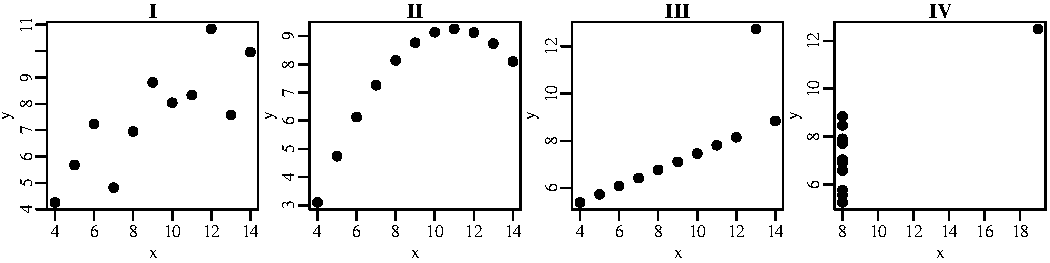
\includegraphics[width=\textwidth]{../figures/anscombe.pdf}
\begingroup
\captionof{figure}{Anscombe's quartet shown as bivariate scatter
  plots.\medskip}\label{fig:anscombe}
\endgroup

Bivariate scatter plots are just one way to visualise analytical data.
Many other graphical devices exist, each of which is appropriate for a
particular type of data. The following sections of this chapter will
introduce a number of these data types, and the associated plots.

\section{Categorical data}
\label{sec:categorical}

Categorical data take one of a limited number of values, assigning
each `object' to a particular class or category. Geological examples
of categorical data are:

\begin{itemize}
\item rock types in a mapping area;
\item animal species in a bone bed;
\item the modal composition of a thin section.
\end{itemize}

Consider, for example, the following 41 clast counts:

\begin{center}
  \begin{tabular}{cccc}
    granite & basalt & gneiss & quartzite \\ \hline
    10 & 5 & 6 & 20  
  \end{tabular}
\end{center}

A bar chart is the natural way to visualise these data:\medskip

\noindent\begin{minipage}[t][][b]{.4\textwidth}
  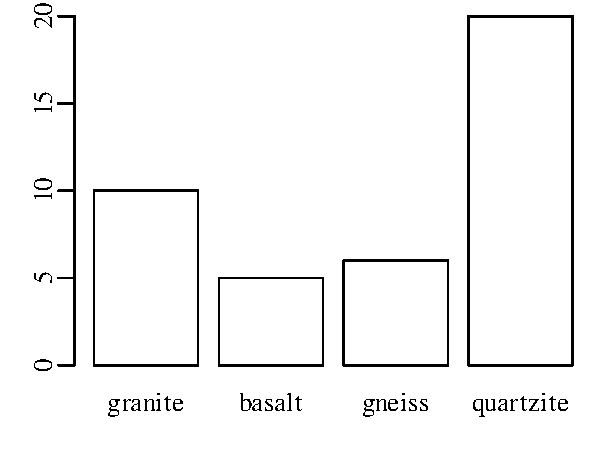
\includegraphics[width=\textwidth]{../figures/clasts.pdf}
\end{minipage}
\begin{minipage}[t][][t]{.6\textwidth}
  \captionof{figure}{Bar chart of clast counts. The vertical axis
    labels the number of objects counted in each category. The order
    of the categories along the horizontal axis is completely
    arbitrary and can be changed without loss of information.}
  \label{fig:clasts}
\end{minipage}

\section{Count data}
\label{sec:counts}

Count data are closely related to categorical data. Geological
examples of this type of data include:

\begin{itemize}
\item the annual number of earthquakes that exceed a certain
  magnitude;
\item the number of gold chips found in a panning session;
\item the number of dry wells in a wildcat drilling survey.
\end{itemize}

The crucial difference between count data and categorical data is that
the order of the categories matters for the count data, whereas it
does not for categorical data.  As an example, consider the number of
earthquakes of magnitude 5.0 or greater between 1917 and 2016:

\noindent\begin{minipage}[t][][b]{.4\textwidth}
  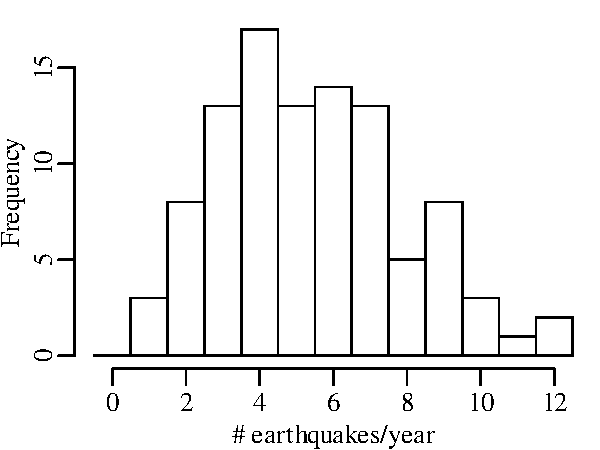
\includegraphics[width=\textwidth]{../figures/declusteredquakesperyear.pdf}
\end{minipage}
\begin{minipage}[t][][t]{.6\textwidth}
  \captionof{figure}{Histogram of magnitude $\geq{5.0}$ earthquakes per
    year between 1917 and 2016. The vertical axis labels the number of
    years. The horizontal axis shows the number of earthquakes. In
    contrast with Figure~\ref{fig:clasts}, the order of the four
    categories along the horizontal axis matters and cannot be changed
    without loss of information. Categorical data whose order matters
    are also known as \emph{ordinal} data.}
  \label{fig:quakecounts}
\end{minipage}

\section{Continuous data}
\label{sec:continuous}

Not all geological or geophysical measurements take integer values.
Many are free to take on any decimal value. A few examples of such
continuous data are:

\begin{itemize}
\item the magnitude of earthquakes;
\item the spontaneous electrical potential between geological strata;
\item the density of minerals;
\item the porosity of a sedimentary rock.
\end{itemize}

Consider the following dataset of pH measurements in 20~samples of
rain water:

\begin{center}
6.2, 4.4, 5.6, 5.2, 4.5, 5.4, 4.8, 5.9, 3.9, 3.8, 5.1, 4.1, 5.1, 5.5,
5.1, 4.6, 5.7, 4.6, 4.6, 5.6
\end{center}

These values can be collected into bins and plotted as a histogram,
just like the count data in section~\ref{sec:counts}. However this
binning exercise poses two practical problems.

\subsection*{i. How many bins should we use, and how wide should they be?}

The number of bins strongly affects the appearance of a histogram:

\noindent\begin{minipage}[t][][b]{.5\textwidth}
  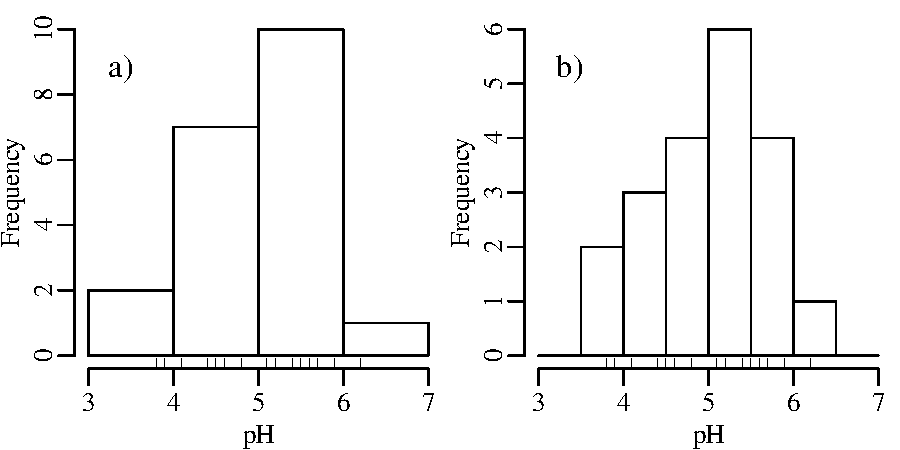
\includegraphics[width=\textwidth]{../figures/binwidth.pdf}\medskip
\end{minipage}
\begin{minipage}[t][][t]{.5\textwidth}
  \captionof{figure}{ Two histograms of the same pH data, with the
    individual measurements marked as vertical ticks underneath. This
    is also known as a \emph{rug plot}, and allows us to better assess
    the effect of bin width on the appearance of histograms.
    Histogram a) uses a bin width of 1~pH unit whereas histogram b)
    uses a bin width of 0.5~pH units. The two histograms look
    considerably different and it is not immediately clear which
    choice of bin width is best.}
  \label{fig:binwidth}
\end{minipage}

A number of rules of thumb are available to choose the optimal number
of bins. For example, \texttt{Excel} uses a simple square root rule:

\begin{equation}
  \mbox{\#{bins} = } \sqrt{n}
\end{equation}

\noindent where $n$ is the number of observations (i.e. $n = 20$ for
the pH example). \texttt{R} uses Sturges' Rule:

\begin{equation}
  \mbox{\#{bins} = } \log_2(n) + 1
\end{equation}

\noindent however no rule of thumb is optimal in all situations.

\subsection*{ii. Where to place the bins?}

Even when the number of bins has been fixed, just shifting them
slightly to the left or to the right can have a significant effect on
the appearance of the histogram. For example:

\noindent\begin{minipage}[t][][b]{.5\textwidth}
  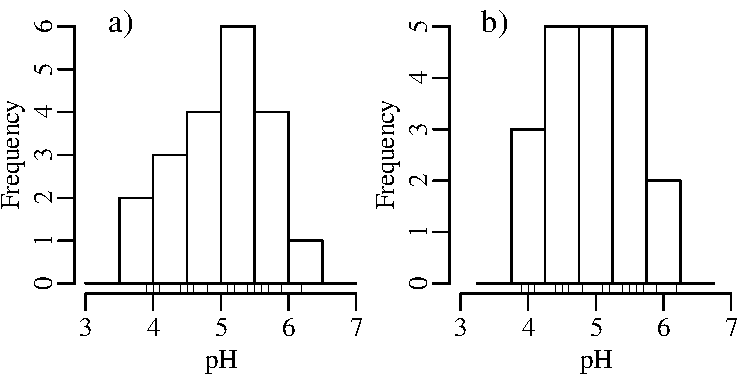
\includegraphics[width=\textwidth]{../figures/binpos.pdf}\medskip
\end{minipage}
\begin{minipage}[t][][t]{.5\textwidth}
  \captionof{figure}{Two histograms of the pH data whose bin widths
    are the same, but whose bins have been offset by 0.25 pH units.
    This arbitrary decision strongly affects the appearance of the
    histogram.}
  \label{fig:binpos}
\end{minipage}
  
To solve the bin placement problem, let us explore a variant of the
ordinary histogram that is constructed as follows:

\begin{enumerate}
\item Rank the measurements from low to high along a line.
\item Place a rectangular `box' on top of each measurement.
\item Stack the boxes to create one connected line.
\end{enumerate}

\noindent\begin{minipage}[t][][b]{.3\textwidth}
  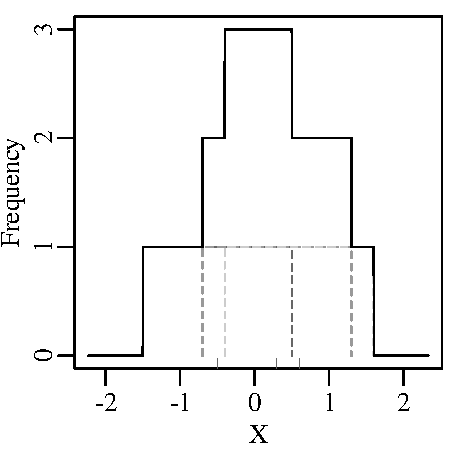
\includegraphics[width=\textwidth]{../figures/rectKDE.pdf}
\end{minipage}
\begin{minipage}[t][][t]{.7\textwidth}
  \captionof{figure}{The rug plot along the bottom axis represents
    three data points. The grey dashed lines mark rectangular boxes
    (`kernels') that are centred around each of these data points. The
    black step function is obtained by taking the sum of these
    boxes. This procedure removes the need to choose bin locations.}
  \label{fig:rectangles}
\end{minipage}

Normalising the area under the resulting curve produces a so-called
Kernel Density Estimate (KDE). The mathematical definition of this
function is:

\begin{equation}
  KDE(x) = \frac{1}{nh} \sum\limits_{i=1}^{n} K\!\left(\frac{x-x_i}{h}\right)
\end{equation}

\noindent where $x_i$ is the $i$\textsuperscript{th} measurement (out
of $n$), $h$ is the `bandwidth' of the kernel density estimator, and
$K(u)$ is the `kernel' function. For the rectangular kernel:

\begin{equation}
  K(u) = 1/2 \mbox{~if~}|u| \leq 1, \mbox{~and~} K(u) = 0 \mbox{~otherwise}
\end{equation}

Applying this method to the pH data:

\noindent\begin{minipage}[t][][b]{.3\textwidth}
  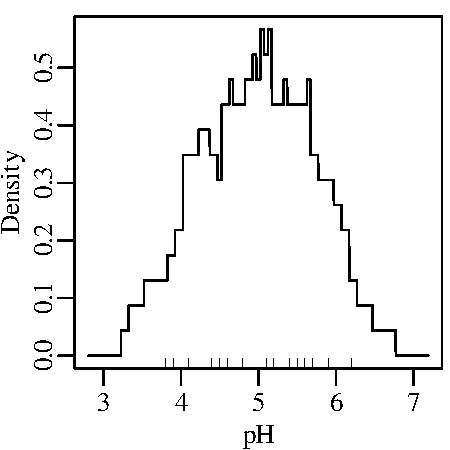
\includegraphics[width=\textwidth]{../figures/pHrectKDE.pdf}
\end{minipage}
\begin{minipage}[t][][t]{.7\textwidth}
  \captionof{figure}{Rectangular KDE of the pH data, constructed using
    the same procedure as shown in Figure~\ref{fig:rectangles}. The
    area under this curve has been normalised to unity.}
  \label{fig:pHrectKDE}
\end{minipage}

Instead of a rectangular kernel, we could also use triangles to
construct the KDE curve, or any other (symmetric) function. One
popular choice is the Gaussian function:

\begin{equation}
  K(u) = \frac{1}{\sqrt{2\pi}}\exp\!\left[-\frac{u^2}{2}\right]
  \label{eq:gaussiankernel}
\end{equation}

\noindent which produces a continuous KDE function:\medskip

\noindent\begin{minipage}[t][][b]{.3\textwidth}
  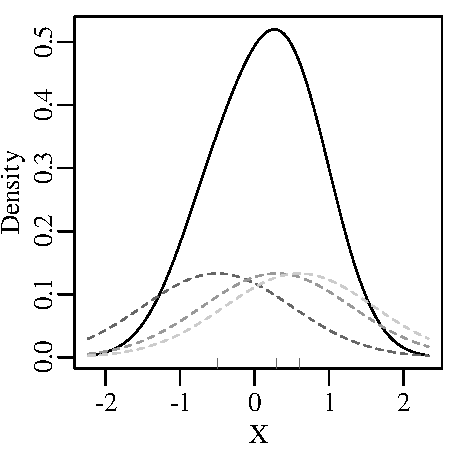
\includegraphics[width=\textwidth]{../figures/gaussKDE.pdf}
\end{minipage}
\begin{minipage}[t][][t]{.7\textwidth}
  \captionof{figure}{Using a Gaussian kernel instead of a rectangular
    kernel on the three data points of Figure~\ref{fig:rectangles}.
    This produces a smooth KDE.}
\end{minipage}

Using the Gaussian kernel to plot the pH data:\medskip

\noindent\begin{minipage}[t][][b]{.3\textwidth}
  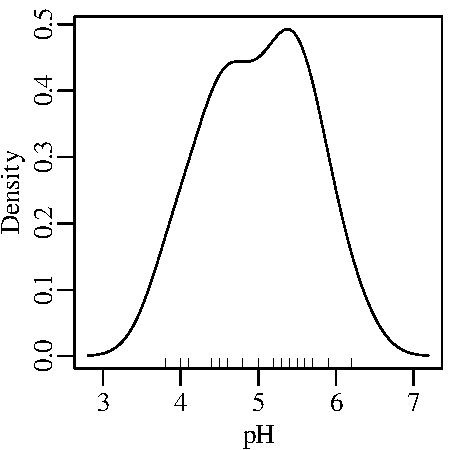
\includegraphics[width=\textwidth]{../figures/pHgaussKDE.pdf}\medskip
\end{minipage}
\begin{minipage}[t][][t]{.7\textwidth}
  \captionof{figure}{Gaussian KDE of the pH data. The continuous curve
    does more justice to the continuous data than the discrete step
    function of Figures~\ref{fig:binwidth}, \ref{fig:binpos} or
    \ref{fig:pHrectKDE}.}
  \label{fig:pHgaussKDE}
\end{minipage}

Although kernel density estimation solves the bin placement problem,
it is not entirely free of design decisions. The bandwidth $h$ of a
KDE fulfils a similar role as the bin width of a histogram. Changes in
$h$ affect the \emph{smoothness} of the KDE curve:\medskip

\noindent\begin{minipage}[t][][b]{.55\textwidth}
  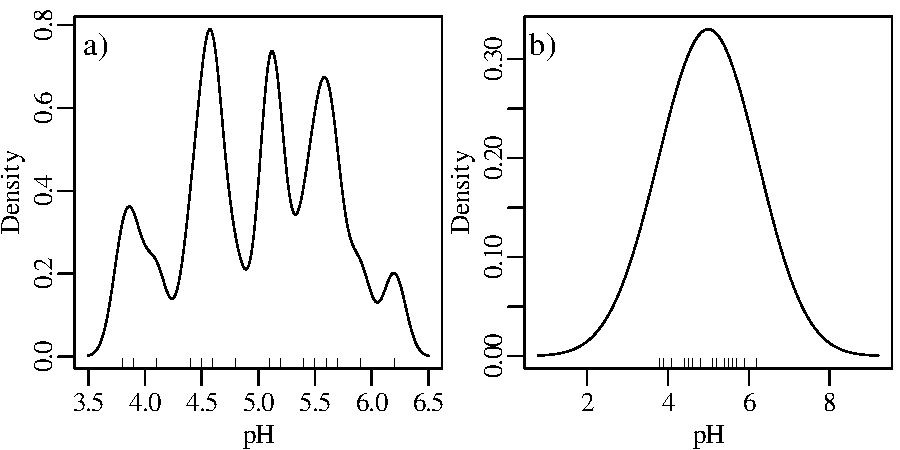
\includegraphics[width=\textwidth]{../figures/bandwidth.pdf}\medskip
\end{minipage}
\begin{minipage}[t][][t]{.45\textwidth}
  \captionof{figure}{KDEs of the pH data with a) a kernel bandwidth of
    $h=0.1$; and b) a bandwidth of $h=1$. Using a narrow bandwidth
    undermooths the data, whereas a wide bandwidth produces an
    oversmoothed distribution.}
\end{minipage}

Bandwidth selection is a similar problem to bin width selection.  A
deeper discussion of this problem falls outside the scope of text.
Suffice it to say that most statistical software (including $R$) use
equivalent rules of thumb to Sturges' Rule to set the bandwidth.  But
these values can be easily overruled by the user.

\section{Data transformations}
\label{sec:transformations}

Consider the following dataset of 20 measurements of sedimentary
clast sizes, in centimetres:

\begin{center}
0.35, 11.00, 6.00, 1.80, 2.30, 0.59, 8.40, 2.90, 5.90, 2.10,\\
1.20, 2.10, 1.10, 1.60, 0.90, 1.70, 3.40, 0.53, 2.20, 7.70
\end{center}

\noindent\begin{minipage}[t][][b]{.3\textwidth}
  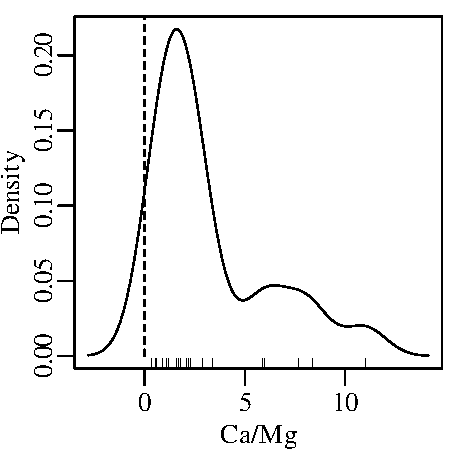
\includegraphics[width=\textwidth]{../figures/negativeKDE.pdf}\medskip
\end{minipage}
\begin{minipage}[t][][t]{.7\textwidth}
  \captionof{figure}{KDE of 20 clast size measurements.  Even though
    all the measurements are strictly positive, the curve extends into
    negative data space.}
  \label{fig:negativeKDE}
\end{minipage}

Clast sizes are strictly positive values. Yet the left tail of the KDE
extends into negative data space, implying that there is a finite
chance of observing negative sizes.  This is clearly nonsense.  In
geophysics, positive quantities are sometimes called \emph{Jeffreys
  quantities} (so named after the British geophysicist Sir Harold
Jeffreys). In addition to length, other examples of Jeffreys
quantities are mass, volume, density, speed, etc. These parameters
exist within an infinite half space between 0 and $+\infty$. We can
transform them to the entire infinite space of numbers by applying a
logarithmic transformation:\medskip

\noindent\begin{minipage}[t][][b]{.6\textwidth}
  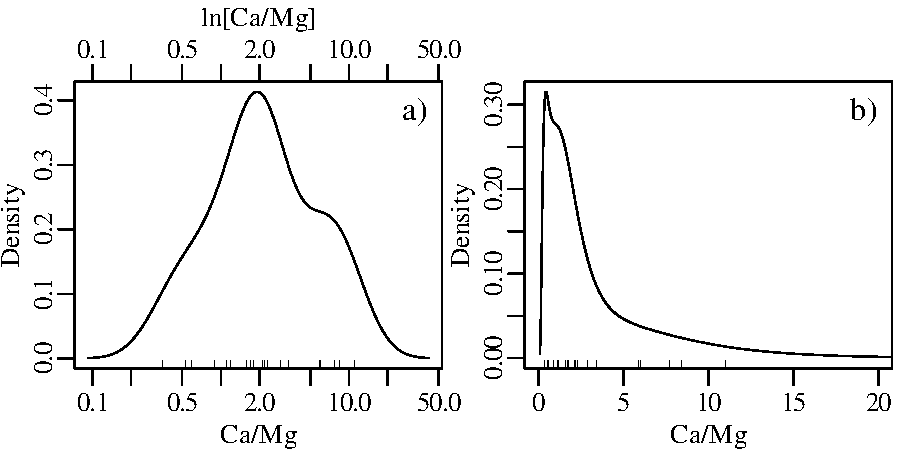
\includegraphics[width=\textwidth]{../figures/logKDE.pdf}\medskip
\end{minipage}
\begin{minipage}[t][][t]{.4\textwidth}
  \captionof{figure}{a) KDE of the clast size measurements, after
    applying a (natural) logarithmic transformation.  Note how the
    distribution has become more symmetric compared to the linear
    scale of Figure~\ref{fig:negativeKDE}. b) The same KDE mapped back
    to linear scale. Unlike Figure~\ref{fig:negativeKDE}, the mapped
    distribution does not cross over into negative values.}
  \label{fig:logKDE}
\end{minipage}

Jeffreys quantities are just one example of constrained measurements.
As another example, consider the following twenty porosity
measurements in limestone:\medskip

\begin{center}
  5.8, 28.0, 12.0, 27.0, 40.0, 12.0, 3.8, 6.3, 17.0, 16.0,\\
  95.0, 94.0, 92.0, 88.0, 88.0, 70.0, 92.0, 72.0, 74.0, 84.0
\end{center}

Porosity takes on values between 0 and 1 (if expressed as fractions,
or between 0 and 100 if expressed as percentages). Yet again the
Gaussian KDE of the data plot into physically impossible values of
$<0$ and $>1$:\medskip

\noindent\begin{minipage}[t][][b]{.3\textwidth}
  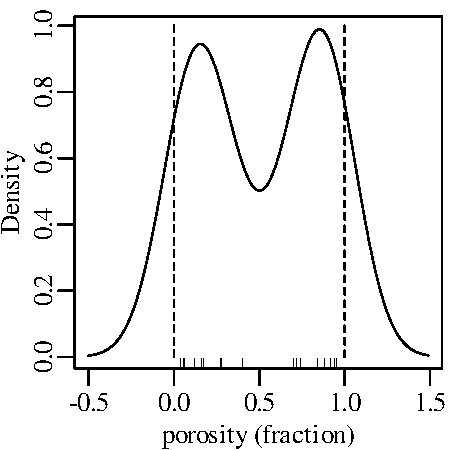
\includegraphics[width=\textwidth]{../figures/porosityKDE.pdf}\medskip
\end{minipage}
\begin{minipage}[t][][t]{.7\textwidth}
  \captionof{figure}{KDE of 20 porosity measurements.  Even though all
    the measurements are between 0 and 1, the KDE extends beyond these
    hard limits.}
  \label{fig:porosityKDE}
\end{minipage}

Using a similar approach as before, the dataspace can be opened up
from the constraints of the 0 to 1 interval to the entire line of
numbers, from $-\infty$ to $+\infty$. For proportions, this is
achieved by the \emph{logistic transformation}:

\begin{equation}
  u = \mbox{logit}(x) = \ln\!\left[\frac{x}{1-x}\right]
  \label{eq:logit}
\end{equation}

After constructing the density estimate (or carrying out any other
numerical manipulation), the results can be mapped back to the 0 to 1
interval with the inverse logit transformation:

\begin{equation}
  x = \mbox{logit}^{-1}(u) = \frac{\exp[u]}{\exp[u]+1}
  \label{eq:invlogit}
\end{equation}

\noindent\begin{minipage}[t][][b]{.6\textwidth}
  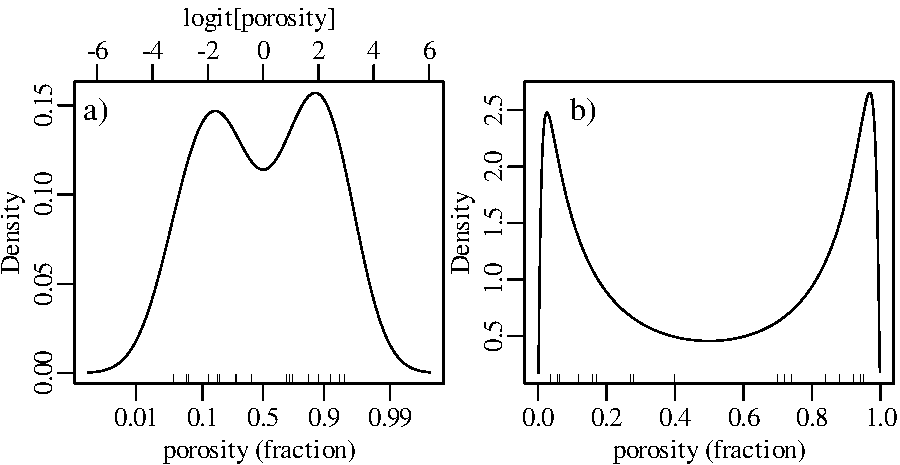
\includegraphics[width=\textwidth]{../figures/logitKDE.pdf}\medskip
\end{minipage}
\begin{minipage}[t][][t]{.4\textwidth}
  \captionof{figure}{a) KDE of the porosity data, after applying a
    logistic transformation.  Note the two horizonal axes.  The top
    axis marks the transformed values on a linear scale that extends
    from $-\infty$ to $+\infty$. The bottom axis is labeled by the
    actual porosity values on a non-linear scale that extends from 0
    to 1. b) The same distribution mapped back to the 0 -- 1
    interval.}
  \label{fig:logitKDE}
\end{minipage}

We will see in chapter~\ref{ch:compositional} that the logistic
transformation is a special case of a general class of \emph{logratio
  transformations} that are useful for the analysis of
\emph{compositional data}.

\section{Multivariate distributions}
\label{sec:multivariate}

KDEs can be generalised from one to two dimensions.  For example,
consider a dataset of eruption timings from the Old Faithful geyser in
Yellowstone national park (Wyoming, USA): \medskip

\noindent\begin{minipage}[t][][b]{.5\textwidth}
  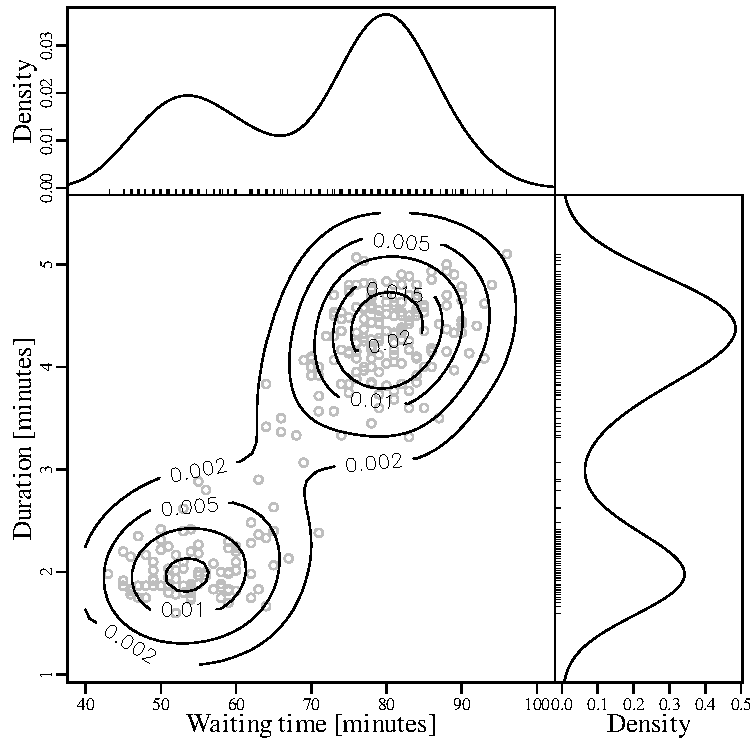
\includegraphics[width=\textwidth]{../figures/KDE2D.pdf}\medskip
\end{minipage}
\begin{minipage}[t][][t]{.5\textwidth}
  \captionof{figure}{Old Faithful eruption measurements. The dataset
    records 272 observations of 2 variables: the duration of each
    eruption, and the waiting time between them. Both variables are
    expressed in minutes. The lower left panel shows the bivariate
    measurements as grey circles. The contour lines represent a
    2-dimensional KDE. The marginal distributions of the waiting times
    (top) and eruption durations (right) are shown as 1-dimensional
    KDEs.}
  \label{fig:KDE2D}
\end{minipage}

It is generally not possible to visualise datasets of more than two
dimensions in a single graphic. In this case there are two options:

\begin{enumerate}
  \item plot the data as a series of 1- or 2-dimensional marginal
    plots; or
  \item extract the most important patterns or trends in the data by
    projection onto a lower dimensional plane. Then show these
    projected data as a lower dimensional graphic.
\end{enumerate}

The second strategy is also known as ``ordination'' and will be
discussed in detail in section~\ref{sec:PCA}.

\section{Empirical cumulative distribution fuctions}
\label{sec:ECDF}

Both histograms and kernel density estimates require the selection of
a `smoothing parameter'. For the histogram, this is the bin width; for
the KDE, it is the bandwidth. Despite the existence of rules thumbs to
automatically choose an appropriate value for the smoothing parameter,
there nevertheless is a level of arbitrariness associated with
them. The empirical cumulative distribution function (ECDF) is an
alternative data visualisation device that does not require
smoothing. An ECDF is step function that jumps up by $1/n$ at each of
$n$ data points.  The mathematical formula for this procedure can be
written as:
  
  \begin{equation}
    F(x) = \sum\limits_{i=1}^{n} 1(x_i<x)/n
    \label{eq:ECDF}
  \end{equation}
 
\noindent where $1(\ast) = 1$ if $\ast$ is `true' and $1(\ast) = 0$ if
$\ast$ is `false'. The y-coordinates of the ECDF are values from 0 to
1 that mark the fraction of the measurements that are less than a
particular value.  Plotting the pH, clast size, porosity and geyser
data as ECDFs:

\noindent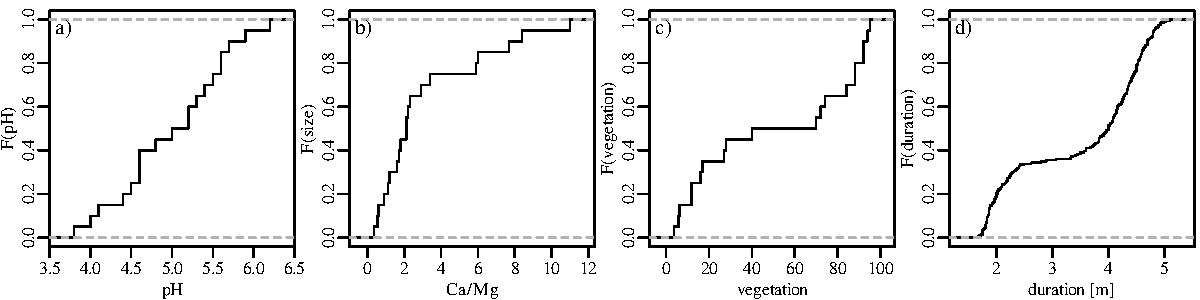
\includegraphics[width=\textwidth]{../figures/ECDFs.pdf}
\begingroup
\captionof{figure}{Empirical cumulative distribution functions (ECDFs)
  of, from left to right: a) the pH data (whose KDE is shown in
  Figure~\ref{fig:pHgaussKDE}); b) the clast size data of
  Figure~\ref{fig:negativeKDE}; c) the porosity data of
  Figure~\ref{fig:porosityKDE}; and d) the eruption time data of
  Figure~\ref{fig:KDE2D}. Note that ECDFs are only applicable to
  1-dimensional datasets.\medskip}
\label{fig:ECDFs}
\endgroup

ECDFs do not require binning or selecting a bandwidth.  Because they
do not require smoothing, they do not spill over into physically
impossible values for the clast size and porosity data. Therefore the
construction of an ECDF is completely hands off.\medskip

The visual interpetation of ECDFs is different from that of histograms
or KDEs. Whereas different clusters of values stand out as `peaks' in
a histogram or KDE, they are marked by steep segments of the ECDF. For
example, the two peaks in the KDE of the geyser data
(Figure~\ref{fig:KDE2D}) correspond to two steps in the ECDF
(Figure~\ref{fig:ECDFs}.d).


\chapter{Summary statistics}
\label{ch:summary-statistics}

After a purely qualitive inspection of the data, we can now move on to
a more quantitive description. This chapter will introduce a number of
\emph{summary statistics} to summarise larger datasets using just a
few numerical values, representing:

\begin{enumerate}
  \item a measure of \emph{location}, representing the `average' of
    the data;
  \item a measure of statistical \emph{dispersion}, quantifying the
    spread of the data; and
  \item a measure of the \emph{shape} of the distribution.
\end{enumerate}

Before proceeding with this topic, it is useful to bear in mind that
these summary statistics have limitations.  The Anscombe quartet of
Table~\ref{tab:anscombe} and Figure~\ref{fig:anscombe} showed that
very different looking datasets can have identical summary
statistics. But with this caveat in mind, summary statistics are an
essential component of data analysis provided that they are preceded
by a visual inspection of the data.

\section{Location}
\label{sec:location}

There are many ways to define the `average' value of a multi-value
dataset.  In this chapter, we will introduce three of these but later
chapters will introduce a few more.

\begin{enumerate}
\item{\bf Mean.} Given a dataset $x = \{x_1,\ldots ,x_i,\ldots, x_n\}$
  comprising $n$ values, the arithmetic mean ($\bar{x}$) is defined
  as:
  \begin{equation}
    \bar{x} = \frac{1}{n}\sum\limits_{i=1}^{n}x_i
    \label{eq:mean}
  \end{equation}
\item{\bf Median.} The median is obtained by ranking the observations
  according to size, and selecting the middle value. If $n$ is an odd
  number, then:

  \begin{equation}
    \mbox{med}(x) = x_1 < \ldots < {\bf x_{n/2}} < \ldots < x_n
  \end{equation}

  If $n$ is an even number, then the median is the average of the two
  numbers on either side of the middle. Graphically, the median can be
  identified as the value that corresponds the to halfway point of the
  ECDF.
  
\item{\bf Mode.} The mode is the most frequently occurring value in a
  dataset. It can be identified as the highest point on a KDE or the
  steepest point on the ECDF.
\end{enumerate}

Applying these three concepts to the pH data, the mean is given by:

\begin{equation*}
  \bar{x} = \frac{
    \begin{array}{c}
      6.2+4.4+5.6+5.2+4.5+5.4+4.8+5.9+3.9+3.8+ \\
      5.1+4.1+5.1+5.5+5.1+4.6+5.7+4.6+4.6+5.6
    \end{array}
  }{20} = 5.00
\end{equation*}

The median is obtained by ranking the values in increasing order, and
marking the two middle values in bold:

\begin{center}
  {3.8, 3.9, 4.1, 4.4, 4.5, 4.6, 4.6, 4.6, 4.8, \textbf{5.1},
  \textbf{5.1}, 5.1, 5.2, 5.4, 5.5, 5.6, 5.6, 5.7, 5.9, 6.2}
\end{center}

Then the median is the average of these two values (median[x] =
5.1). Finally, the mode is the pH value that corresponds to the
maximum value of the KDE (mode[x]=5.25):

\noindent\begin{minipage}[t][][b]{.5\textwidth}
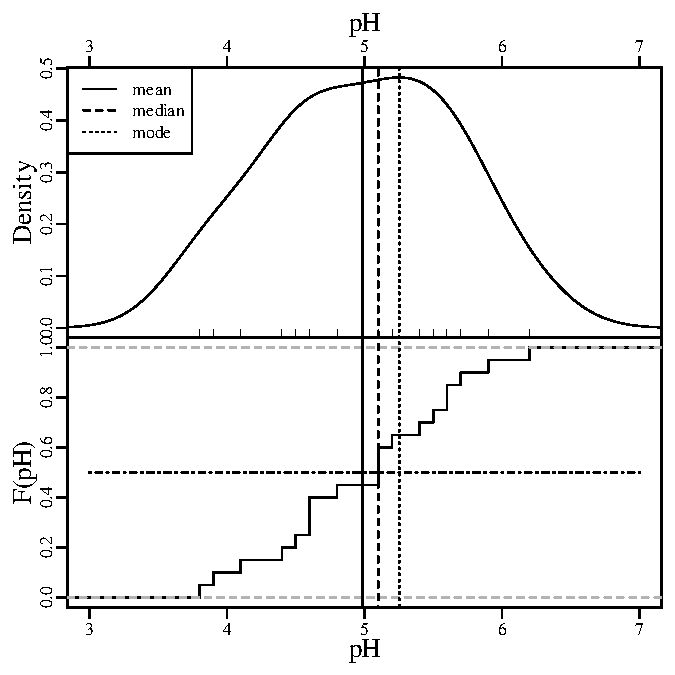
\includegraphics[width=\textwidth]{../figures/pHlocation.pdf}
\end{minipage}
\begin{minipage}[t][][t]{.5\textwidth}
  \captionof{figure}{Rug plot (top) and ECDF (bottom) of the pH
    data. The mean (solid vertical line) is 5.00, the median (dashed
    line) is 5.10 and the mode (dotted line) is 5.25. The dash-dot
    line on the bottom panel marks halfway mark of the ECDF. The
    intersection of this line with the ECDF marks the median. All
    three measures of location are closely spaced together in the
    densest part of the dataset.}
\end{minipage}

Calculating the same three summary statistics for the clast size data:

\noindent\begin{minipage}[t][][b]{.5\textwidth}
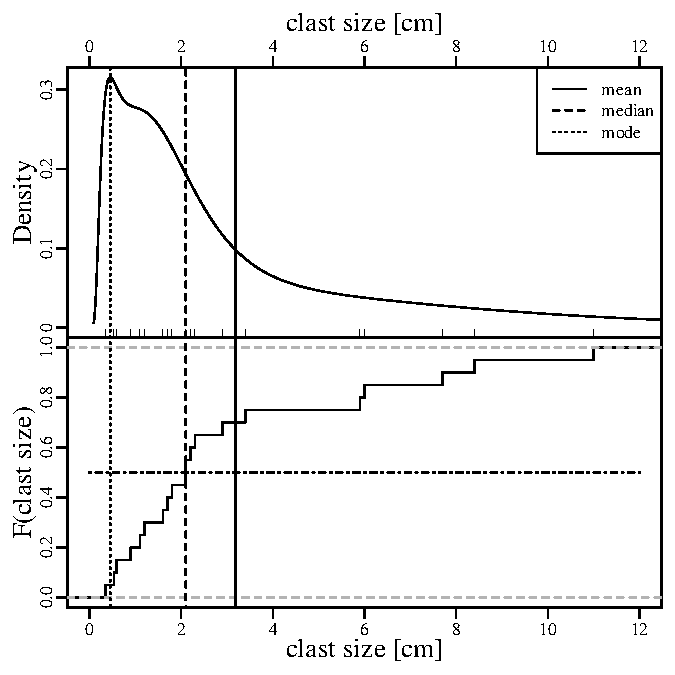
\includegraphics[width=\textwidth]{../figures/clastslocation.pdf}
\end{minipage}
\begin{minipage}[t][][t]{.5\textwidth}
  \captionof{figure}{Rug plot and ECDF of the clast size data. The
    mean (solid vertical line) is 3.19, the median (dashed line) is
    2.1, and the mode (dotted line) is 0.45. There is a factor 7
    difference between the smallest and largest measure of location
    for this dataset. The mean is strongly affected by the long `tail'
    of large outliers. Only 6 out of 20 clasts (30\%) are larger than
    the mean of the distribution and only 1 is (5\%) is smaller than
    the mode.}
  \label{fig:clastslocation}
\end{minipage}
\vfill
Finally, repeating the exercise one more time for the porosity and
geyser eruption data:

\noindent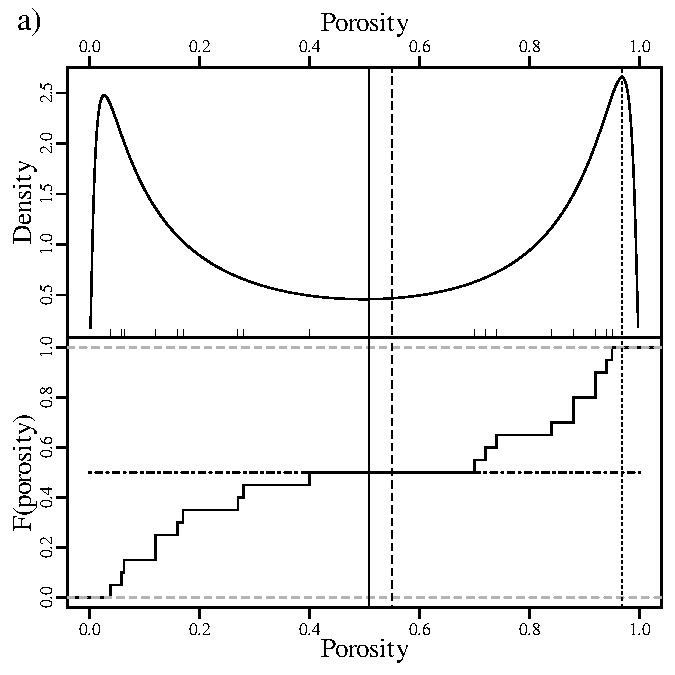
\includegraphics[width=.5\textwidth]{../figures/porositylocation.pdf}
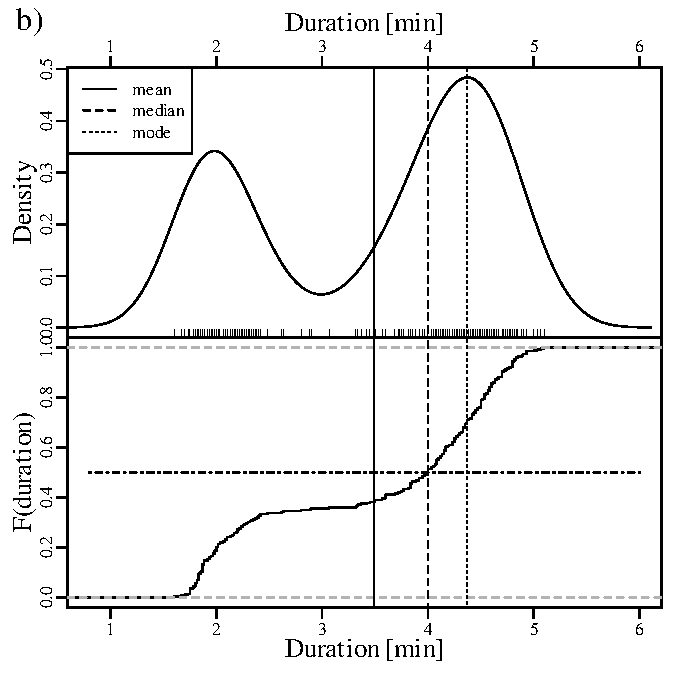
\includegraphics[width=.5\textwidth]{../figures/eruptionslocation.pdf}
\begingroup
\captionof{figure}{Rug plot and ECDF of a) the porosity data (mean =
  0.51, median = 0.55, mode = 0.97); and b) the geyser eruption data
  (mean = 3.49, median = 4.0, mode = 4.37). Both of these
  distributions are `bimodal', meaning that they have two `peaks' in
  the KDE, corresponding to two steep segments in the ECDFs. The
  dotted lines mark the highest one of them and ignores the other
  one. The mean and median fall in between the two modes and are not
  representative of the data.\\}
\label{fig:porositylocation}
\endgroup

Comparing the three sets of examples leads to the following
conclusions:

\begin{enumerate}
\item the mean is a meaningful measure of location for unimodal and
  symmetric distribution;
\item the mean is more strongly affected by outliers than the median;
\item therefore the median is more a more robust estimator of location
  for asymmetric datasets;
\item multimodal datasets cannot be adequately summarised with a
  single location parameter.
\end{enumerate}

\section{Dispersion}
\label{sec:dispersion}

It is rare for all the values in a dataset to be exactly the same. In
most cases they are spread out over a finite range of values. The
amount of spread can be defined in a number of ways, the most common
of which are:

\begin{enumerate}

\item{\bf Standard deviation.} Given $n$ measurements $x_i$ (for $1
  \leq i \leq n$), the standard deviation is defined as:

\begin{equation}
  s[x] = \sqrt{\frac{1}{n-1}\sum\limits_{i=1}^{n}(x_i-\bar{x})^2}
  \label{eq:stdev}
\end{equation}

\noindent where $\bar{x}$ is the arithmetic mean
(Equation~\ref{eq:mean}). The square of the standard deviation
(i.e. $s[x]^2$) is also known as the \textbf{variance}.

\item{\bf Median Absolute Deviation (MAD).} Whereas the standard
  deviation quantifies the dispersion around the mean, MAD quantifies
  the dispersion around the median:

  \begin{equation}
    \mbox{MAD} = \mbox{median}|x_i - \mbox{median}(x)|
    \label{eq:MAD}
  \end{equation}

  \noindent where `$|\ast|$' stands for ``the absolute value of
  $\ast$''.
  
\item{\bf Interquartile range (IQR).} The ECDF can be used to define
  the \textbf{quantiles} of a sample distribution. For example, the
  0.1 quantile (or 10\textsuperscript{th} \textbf{percentile}) of the
  pH data is 3.9, because 10\% of the pH values are $\leq$3.9. Thus,
  the median is equivalent to the ``0.5 quantile'' or the ``50
  percentile''. The 25, 50 and 75 percentiles are also known as the
  \textbf{quartiles}. The IQR marks the difference between the third
  and the first quantile (i.e., 25 and 75 percentile).
  
\end{enumerate}

Calculating the standard deviation of the pH data (whose mean is
$\bar{x} = 5.0$):

\begin{center}
\begin{tabular}{c@{\tgap}|
    @{\tgap}c@{\gap}c@{\gap}c@{\gap}c@{\gap}c@{\tgap}
    @{\tgap}c@{\gap}c@{\gap}c@{\gap}c@{\gap}c@{\tgap}
    @{\tgap}c@{\gap}c@{\gap}c@{\gap}c@{\gap}c@{\tgap}
    @{\tgap}c@{\gap}c@{\gap}c@{\gap}c@{\gap}c@{\tgap}}
  $i$ & 1 & 2 & 3 & 4 & 5 & 6 & 7 & 8 & 9 & 10 &
  11 & 12 & 13 & 14 & 15 & 16 & 17 & 18 & 19 & 20 \\ \hline
  $x_i$ & 6.2 & 4.4 & 5.6 & 5.2 & 4.5 & 5.4 & 4.8 & 5.9 & 3.9 & 3.8 & 
  5.1 & 4.1 & 5.1 & 5.5 & 5.1 & 4.6 & 5.7 & 4.6 & 4.6 & 5.6 \\
  $(x_i-\bar{x})$ & 1.20 & -.58 & .61 & .21 & -.49 & .42 &
  -.19 & .92 & -1.1 & -1.2 & .11 & -.89 & .11 & .51 &
  .11 & -.39 & .71 & -.39 & -.39 & .61 \\
  $(x_i-\bar{x})^2$ & 1.5 & .34 & .38 & .046 & .24 & .17 &
  .034 & .84 & 1.2 & 1.4 & .013 & .78 & .013 & .27 & .013 &
  .15 & .51 & .15 & .15 & .38
\end{tabular}
\end{center}

Taking the sum of the last row:

\[
\sum\limits_{i=1}^{20} (x_i-\bar{x})^2 = 8.52
\]

\noindent from which we get:

\[
s[x] = \sqrt{8.52/19} = 0.70
\]

Sorting the pH values in increasing order and recalling that med$(x) = 5.1$:

\begin{center}
\begin{tabular}{c@{\tgap}|
    @{\tgap}c@{\gap}c@{\gap}c@{\gap}c@{\gap}c@{\tgap}|
    @{\tgap}c@{\gap}c@{\gap}c@{\gap}c@{\gap}c@{\tgap}|
    @{\tgap}c@{\gap}c@{\gap}c@{\gap}c@{\gap}c@{\tgap}|
    @{\tgap}c@{\gap}c@{\gap}c@{\gap}c@{\gap}c@{\tgap}} $i$ & 1 & 2 & 3
  & 4 & 5 & 6 & 7 & 8 & 9 & 10 & 11 & 12 & 13 & 14 & 15 & 16 & 17 & 18
  & 19 & 20 \\ \hline
  $x_i$ & 3.8 & 3.9 & 4.1 & 4.4 & \textbf{4.5} &
  \textbf{4.6} & 4.6 & 4.6 & 4.8 & 5.1 & 5.1 & 5.1 & 5.2 & 5.4 &
  \textbf{5.5} & \textbf{5.6} & 5.6 & 5.7 & 5.9 & 6.2 \\
  $x_i-\mbox{med}(x)$ & -1.3 & -1.2 & -1.0 & -0.7 & -0.6 & -0.5 &
  -0.5 & -0.5 & -0.3 & 0.0 & 0.0 & 0.0 & 0.1 & 0.3 & 0.4 & 0.5 & 0.5 &
  0.6 & 0.8 & 1.1 \\
  $|x_i-\mbox{med}(x)|$ & 1.3 & 1.2 & 1.0 & 0.7 &
  0.6 & 0.5 & 0.5 & 0.5 & 0.3 & 0.0 & 0.0 & 0.0 & 0.1 & 0.3 & 0.4 &
  0.5 & 0.5 & 0.6 & 0.8 & 1.1 \\
  sorted & 0.0 & 0.0 & 0.0 & 0.1 & 0.3
  & 0.3 & 0.4 & 0.5 & 0.5 & \textbf{0.5} & \textbf{0.5} & 0.5 & 0.6 &
  0.6 & 0.7 & 0.8 & 1.0 & 1.1 & 1.2 & 1.3
\end{tabular}
\end{center}

The MAD is given by the mean of the bold values on the final row of
this table, yielding a value of MAD = 0.5.\\

The 25 and 75 percentiles are obtained by averaging the two pairs of
bold faced numbers on the second row of the table. They are 4.55 and
5.55, respectively. Therefore, IQR = 5.55 - 4.55 = 1.00. Showing the
same calculation on an ECDF:

\noindent\begin{minipage}[t][][b]{.4\textwidth}
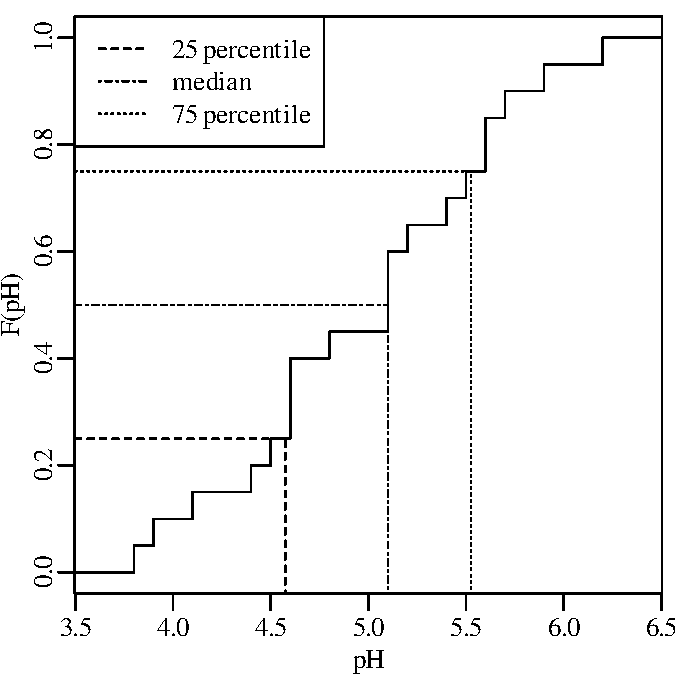
\includegraphics[width=\textwidth]{../figures/IQRpH.pdf}
\end{minipage}
\begin{minipage}[t][][t]{.6\textwidth}
  \captionof{figure}{ECDF of the pH data with indication of the three
    quantiles, namely the 25 percentile, median and 75 percentile.
    The Interquartile Range (IQR) is defined as the difference between
    the 75 and 25 percentiles. This is 1 pH unit in this example.  The
    standard deviation and Median Absolute Deviation are $s[x] = 0.7$
    and MAD = 0.5 pH units, respectively.}
\end{minipage}

\section{Shape}
\label{sec:shape}

The \textbf{skewness} of a distribution is defined as:

\begin{equation}
  \mbox{skew}(x) = \frac{1}{n \cdot s[x]^3}\sum\limits_{i=1}^{n}(x_i-\bar{x})^3
  \label{eq:skew}
\end{equation}

To assess the meaning of this new summary statistic, let us plot the
pH and clast size datasets alongside the distribution of Covid-19
death rates (in deaths per 100,000 people) in the UK:\\

\noindent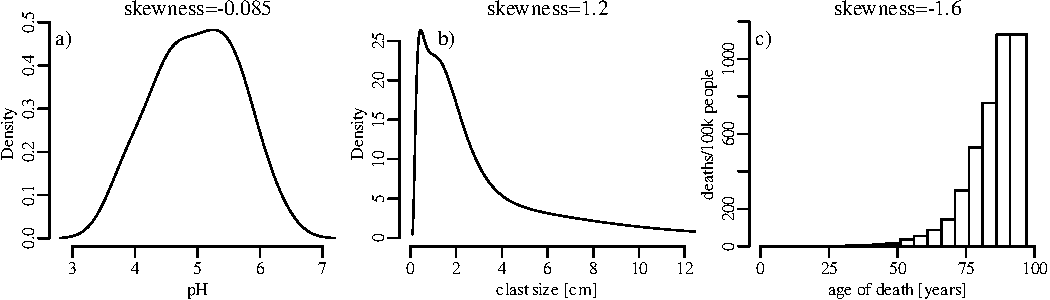
\includegraphics[width=\textwidth]{../figures/skewness.pdf}
\begingroup
  \captionof{figure}{a) the frequency distributions of pH data is
    symmetric and is characterised by a near zero (but ever so slightly
    negative) skewness; b) the clast size measurements are positively
    skewed, i.e. they heavily lean towards small values with a heavy
    `tail' of higher values; c) finally, the distribution of Covid-19
    death rates in the UK is negatively skewed: old people are much more
    likely to die of covid than young people.\\}
\endgroup

Note that all the aforementioned summary statistics are strongly
\emph{scale dependent}. The skewness of the Covid-19 data is not only
large because the distribution is very skewed, but also because it
contains numbers (0$<$age$<$100~years) that are an order of magnitude
larger than the numerical values in the pH (3$<$pH$<$7) and clast
size (0$<$size$<$12~cm) datasets.

\section{Box-and-whisker plots}
\label{sec:boxplots}

A box-and-wisker plot is a compact way to jointly visualise the most
important summary statistics in a dataset:

\begin{enumerate}
\item a box is drawn from the first to the third quartile (i.e. from
  the 25 to the 75 percentile);
\item the median is marked by a horizontal line in the middle of the box;
\item two lines extend from the box towards the minimum and maximum
  value, ignoring outliers (as defined next);
\item any points that fall more than 1.5 times the IQR below the first
  quartile, or more than 1.5 times the IQR above the third quartile
  are marked as outliers.
\end{enumerate}

\noindent\begin{minipage}[t][][b]{.45\textwidth}
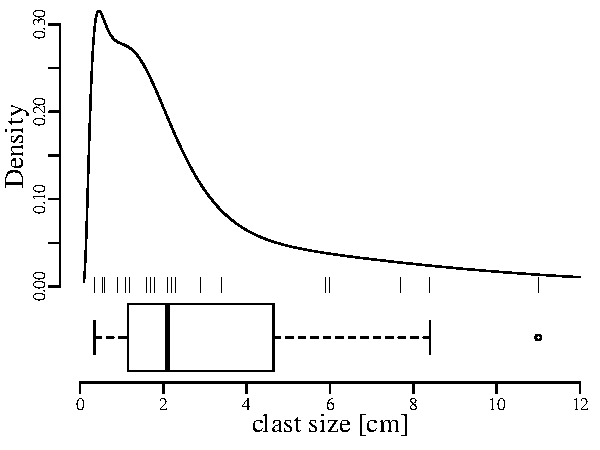
\includegraphics[width=\textwidth]{../figures/boxplot.pdf}
\end{minipage}
\begin{minipage}[t][][t]{.55\textwidth}
  \captionof{figure}{KDE (top) and box-and-whisker plot (bottom) of
    the clast size data. The width of the box marks the IQR.  The
    whiskers extend to the minimum and maximum value, excluding a
    single outlier which, at $\sim$11cm, is more than 1.5 IQR larger
    than the third quartile (75 percentile). The median is offset
    towards the left hand side of the box, indicating the positive
    skewness of the datasets.}
\end{minipage}


\chapter{Probability}
\label{ch:probability}

Probability is a numerical description of how likely it is for an
event to occur or how likely it is for a proposition to be true.  In
the context of a random experiment, in which all outcomes are equally
likely, the probability of an outcome $A$ can be defined as:
\begin{equation}
P(A) = \frac{\mbox{the number of ways }A\mbox{ can occur}}
{\mbox{the total number of outcomes}}
\end{equation}

For example, the probability of tossing an unbiased coin and observing
a head ($H$) is
\[
\frac{
  \{H\}
}{
  \{H\}\{T\}
} = \frac{1}{2} = 0.5
\]

The probability of tossing the same coin three times and obtaining two
heads and one tail ($T$) is:
\begin{equation}
  P(H,H,T) =
  \frac{
    \{THH\}\{HTH\}\{HHT\}
  }{
    \{HHH\}\{THH\}\{HTH\}\{HHT\}\{TTH\}\{THT\}\{HTT\}\{TTT\}
  } = \frac{3}{8}
  \label{eq:2H1T}
\end{equation}

Similarly, the probability of throwing two fair dice and obtaining a
two (\raisebox{-2pt}{\Cube{2}}) and a six (\raisebox{-2pt}{\Cube{6}})
is:
\begin{equation}
  P\!\left(\mbox{\raisebox{-2pt}{\Cube{2}},\raisebox{-2pt}{\Cube{6}}}\right) =
  \frac{
    \mbox{
      \big\{\raisebox{-2pt}{\Cube{2} \Cube{6}}\big\}\big\{\raisebox{-2pt}{\Cube{6} \Cube{2}}\big\}
    }
  }{
    \begin{array}{c}
      \mbox{
        \big\{\raisebox{-2pt}{\Cube{1} \Cube{1}}\big\}\big\{\raisebox{-2pt}{\Cube{2} \Cube{1}}\big\}\big\{\raisebox{-2pt}{\Cube{3} \Cube{1}}\big\}\big\{\raisebox{-2pt}{\Cube{4} \Cube{1}}\big\}\big\{\raisebox{-2pt}{\Cube{5} \Cube{1}}\big\}\big\{\raisebox{-2pt}{\Cube{6} \Cube{1}}\big\}
      }\\
      \mbox{
        \big\{\raisebox{-2pt}{\Cube{1} \Cube{2}}\big\}\big\{\raisebox{-2pt}{\Cube{2} \Cube{2}}\big\}\big\{\raisebox{-2pt}{\Cube{3} \Cube{2}}\big\}\big\{\raisebox{-2pt}{\Cube{4} \Cube{2}}\big\}\big\{\raisebox{-2pt}{\Cube{5} \Cube{2}}\big\}\big\{\raisebox{-2pt}{\Cube{6} \Cube{2}}\big\}
      }\\
      \mbox{
        \big\{\raisebox{-2pt}{\Cube{1} \Cube{3}}\big\}\big\{\raisebox{-2pt}{\Cube{2} \Cube{3}}\big\}\big\{\raisebox{-2pt}{\Cube{3} \Cube{3}}\big\}\big\{\raisebox{-2pt}{\Cube{4} \Cube{3}}\big\}\big\{\raisebox{-2pt}{\Cube{5} \Cube{3}}\big\}\big\{\raisebox{-2pt}{\Cube{6} \Cube{3}}\big\}
      }\\
      \mbox{
        \big\{\raisebox{-2pt}{\Cube{1} \Cube{4}}\big\}\big\{\raisebox{-2pt}{\Cube{2} \Cube{4}}\big\}\big\{\raisebox{-2pt}{\Cube{3} \Cube{4}}\big\}\big\{\raisebox{-2pt}{\Cube{4} \Cube{4}}\big\}\big\{\raisebox{-2pt}{\Cube{5} \Cube{4}}\big\}\big\{\raisebox{-2pt}{\Cube{6} \Cube{4}}\big\}
      }\\
      \mbox{
        \big\{\raisebox{-2pt}{\Cube{1} \Cube{5}}\big\}\big\{\raisebox{-2pt}{\Cube{2} \Cube{5}}\big\}\big\{\raisebox{-2pt}{\Cube{3} \Cube{5}}\big\}\big\{\raisebox{-2pt}{\Cube{4} \Cube{5}}\big\}\big\{\raisebox{-2pt}{\Cube{5} \Cube{5}}\big\}\big\{\raisebox{-2pt}{\Cube{6} \Cube{5}}\big\}
      }\\
      \mbox{
        \big\{\raisebox{-2pt}{\Cube{1} \Cube{6}}\big\}\big\{\raisebox{-2pt}{\Cube{2} \Cube{6}}\big\}\big\{\raisebox{-2pt}{\Cube{3} \Cube{6}}\big\}\big\{\raisebox{-2pt}{\Cube{4} \Cube{6}}\big\}\big\{\raisebox{-2pt}{\Cube{5} \Cube{6}}\big\}\big\{\raisebox{-2pt}{\Cube{6} \Cube{6}}\big\}
      }
    \end{array}
  } = \frac{2}{36} = \frac{1}{18}
  \label{eq:1116}
\end{equation}

The \textbf{multiplicative rule of
  probability}\label{page:multiplication} states that the probability
of two combined \emph{independent}\footnote{Independent means that the
outcome of the first experiment does not depend on the outcome of the
second. The case of non-independent experiments will be discussed in
Section~\ref{sec:conditionalprobability}.} experiments is given by the
product of their respective probabilities. Thus, if one were to carry
out a coin tossing \emph{and} a dice throwing experiment, then the
probability of obtaining two heads and one tail for the first
experiment \emph{and} throwing a two and a six in the second
experiment is:
\[
P\!\left(H,H,T \cap \mbox{\raisebox{-2pt}{\Cube{2}},\raisebox{-2pt}{\Cube{6}}}
\right) =
\frac{3}{8}\frac{1}{18} = \frac{3}{144} = 0.021
\]

\noindent where $\cap$ stands for `and' in the sense of ``the
intersection of two sets of outcomes''. Similarly, the likelihood of
throwing an unbiased coin twice and obtaining two heads can be
calculated as:
\[
P(H \cap H) = \frac{1}{2}\frac{1}{2} = \frac{1}{4}
\]

The \textbf{additive rule of probability}\label{page:addition} states
that the probability of observing \emph{either} of two outcomes $A$
and $B$ is given by:
\begin{equation}
  P({A}\cup{B}) = P(A) + P(B) - P({A}\cap{B})
  \label{eq:additive}
\end{equation}

For example the probability of observing two heads for the first
experiment \emph{or} throwing a two and a six in the second experiment
is:
\[
P\left(H,H,T \cup \mbox{\raisebox{-2pt}{\Cube{2}},\raisebox{-2pt}{\Cube{6}}}\right) =
\frac{3}{8} + \frac{1}{18} - \frac{3}{144} = \frac{59}{144} = 0.410
\]

For two mutually exclusive experiments, the third term in
Equation~\ref{eq:additive} disappears. For example, the probability of
obtaining two heads and one tail \emph{or} throwing three heads is:
\[
P\left(H,H,T \cup H,H,H\right) = \frac{3}{8} + \frac{1}{8} = \frac{4}{8} = 0.5
\]

\section{Permutations}
\label{sec:permutations}

A permutation is an ordered arrangement of objects. These objects can
be selected in one of two ways:

\begin{enumerate}
\item{\bf sampling with replacement.} Consider an urn with $n$ balls
  that are numbered 1 through $n$. Draw a ball from the urn and write
  down its number. There are $n$ possible outcomes for this
  experiment.  Then place the ball back in the urn, thoroughly mix the
  balls and draw a second one. Write down its number. There are $n$
  possible outcomes for the second experiment. Using the
  multiplicative rule of probability, there are $(n\times{n})$
  possible outcomes for the two numbers. Repeat until you have drawn
  $k$ balls. Then the number of possible sequences of numbers is
  \begin{equation}
  \overset{k \mbox{~times}}{\overbrace{n\times{n}\times{\ldots}\times{n}}} = n^k
  \end{equation}
  
\item{\bf sampling without replacement.} Consider the same urn as
  before and draw a first number. Like before, there are $n$ possible
  outcomes.  However this time we do not put the ball back into the
  urn. With the first ball removed, draw a second number. This time
  there are only $(n - 1)$ possible outcomes. Thus, the total number
  of outcomes for the first two numbers is $n \times
  (n-1)$. Continuing the experiment until you have drawn $k$ balls
  (where $k \leq n$) yields
  \begin{equation}
  n\times(n-1)\times(n-2)\times{\ldots}\times(n-k+1) = \frac{n!}{(n-k)!}
  \end{equation}
  possible sequences, where `!' is the factorial operator.

\end{enumerate}

Let us apply these two formulas to a classic statistical problem:
``\textit{what is the probability that at least two students in a
  classroom of k celebrate their birthdays on the same day?}''. The
solution is as follows.

\begin{enumerate}
\item There are ($n=$) 365 possible days on which the first person might
  celebrate their birthday.
\item There are 365 possible days on which the second person might
  celebrate their birthday, but only 364 of these do not overlap with
  the first person's birthday.
\item There are another 365 possible days on which the third person
  might celebrate their birthday, but only 363 of these do not overlap
  with the birthdays of the first two people.
\item For $k$ people, there are $365^k$ possible sets of birthdays
  (sampling with replacement), but only
  $365\times{364}\times{\ldots}(k+1) = 365!/(365-k)!$ of these sets do
  not overlap (sampling without replacement).
\item Therefore, the probability that two people's birthdays do
  not overlap is given by
  \[
  P(\mbox{no overlapping birthdays}) = \frac{365!}{(365-k)!365^k}
  \]
\item And the probability that at least two people's birthdays
  overlap is
  \[
  P(>1~\mbox{overlapping birthdays}) = 1 - \frac{365!}{(365-k)!365^k}
  \]  
\end{enumerate}

If $k = 23$, then $P(>1~\mbox{overlapping birthdays}) = 0.507$. In
other words, there is a greater than 50\% chance that at least two
students will share the same birthday in a classroom of 23.

\section{Combinations}
\label{sec:combinations}

Section~\ref{sec:permutations} showed that there are $n^k$ unique
possible ways to select $k$ objects from a collection of $n$ with
replacement. For example, there are $2^3=8$ ways for three coins to
land:
\[\{HHH\}\{THH\}\{HTH\}\{HHT\}\{TTH\}\{THT\}\{HTT\}\{TTT\}\]

\noindent and there are $6^2=36$ ways for two dice to land:
\[
\begin{array}{c}
\mbox{ \big\{\raisebox{-2pt}{\Cube{1}
    \Cube{1}}\big\}\big\{\raisebox{-2pt}{\Cube{2}
    \Cube{1}}\big\}\big\{\raisebox{-2pt}{\Cube{3}
    \Cube{1}}\big\}\big\{\raisebox{-2pt}{\Cube{4}
    \Cube{1}}\big\}\big\{\raisebox{-2pt}{\Cube{5}
    \Cube{1}}\big\}\big\{\raisebox{-2pt}{\Cube{6} \Cube{1}}\big\}
}\\ \mbox{ \big\{\raisebox{-2pt}{\Cube{1}
    \Cube{2}}\big\}\big\{\raisebox{-2pt}{\Cube{2}
    \Cube{2}}\big\}\big\{\raisebox{-2pt}{\Cube{3}
    \Cube{2}}\big\}\big\{\raisebox{-2pt}{\Cube{4}
    \Cube{2}}\big\}\big\{\raisebox{-2pt}{\Cube{5}
    \Cube{2}}\big\}\big\{\raisebox{-2pt}{\Cube{6} \Cube{2}}\big\}
}\\ \mbox{ \big\{\raisebox{-2pt}{\Cube{1}
    \Cube{3}}\big\}\big\{\raisebox{-2pt}{\Cube{2}
    \Cube{3}}\big\}\big\{\raisebox{-2pt}{\Cube{3}
    \Cube{3}}\big\}\big\{\raisebox{-2pt}{\Cube{4}
    \Cube{3}}\big\}\big\{\raisebox{-2pt}{\Cube{5}
    \Cube{3}}\big\}\big\{\raisebox{-2pt}{\Cube{6} \Cube{3}}\big\}
}\\ \mbox{ \big\{\raisebox{-2pt}{\Cube{1}
    \Cube{4}}\big\}\big\{\raisebox{-2pt}{\Cube{2}
    \Cube{4}}\big\}\big\{\raisebox{-2pt}{\Cube{3}
    \Cube{4}}\big\}\big\{\raisebox{-2pt}{\Cube{4}
    \Cube{4}}\big\}\big\{\raisebox{-2pt}{\Cube{5}
    \Cube{4}}\big\}\big\{\raisebox{-2pt}{\Cube{6} \Cube{4}}\big\}
}\\ \mbox{ \big\{\raisebox{-2pt}{\Cube{1}
    \Cube{5}}\big\}\big\{\raisebox{-2pt}{\Cube{2}
    \Cube{5}}\big\}\big\{\raisebox{-2pt}{\Cube{3}
    \Cube{5}}\big\}\big\{\raisebox{-2pt}{\Cube{4}
    \Cube{5}}\big\}\big\{\raisebox{-2pt}{\Cube{5}
    \Cube{5}}\big\}\big\{\raisebox{-2pt}{\Cube{6} \Cube{5}}\big\}
}\\ \mbox{ \big\{\raisebox{-2pt}{\Cube{1}
    \Cube{6}}\big\}\big\{\raisebox{-2pt}{\Cube{2}
    \Cube{6}}\big\}\big\{\raisebox{-2pt}{\Cube{3}
    \Cube{6}}\big\}\big\{\raisebox{-2pt}{\Cube{4}
    \Cube{6}}\big\}\big\{\raisebox{-2pt}{\Cube{5}
    \Cube{6}}\big\}\big\{\raisebox{-2pt}{\Cube{6} \Cube{6}}\big\}
}
\end{array}\]
    
Note that these are the denominators of the two examples that were
given in the introductory paragraph of this chapter. Also note that
the collection of outcomes contains quite a few duplicate values if
one ignores the order.  For the coin example, these fall into two
groups of three duplicates:
\[\{\{HTT\}\{THT\}\{HHT\}\} \mbox{~and~} \{\{THH\}\{HTH\}\{TTH\}\}\]

For the dice, there are fifteen groups of duplicate pairs:
\[
\begin{array}{l}
  \big\{
  \big\{\raisebox{-2pt}{\Cube{1} \Cube{2}}\big\}
  \big\{\raisebox{-2pt}{\Cube{2} \Cube{1}}\big\}
  \big\}
  \big\{
  \big\{\raisebox{-2pt}{\Cube{1} \Cube{3}}\big\}
  \big\{\raisebox{-2pt}{\Cube{3} \Cube{1}}\big\}
  \big\}
  \big\{
  \big\{\raisebox{-2pt}{\Cube{1} \Cube{4}}\big\}
  \big\{\raisebox{-2pt}{\Cube{4} \Cube{1}}\big\}
  \big\}
  \big\{
  \big\{\raisebox{-2pt}{\Cube{1} \Cube{5}}\big\}
  \big\{\raisebox{-2pt}{\Cube{5} \Cube{1}}\big\}
  \big\}
  \big\{
  \big\{\raisebox{-2pt}{\Cube{1} \Cube{6}}\big\}
  \big\{\raisebox{-2pt}{\Cube{6} \Cube{1}}\big\}
  \big\}\\
  \big\{
  \big\{\raisebox{-2pt}{\Cube{2} \Cube{3}}\big\}
  \big\{\raisebox{-2pt}{\Cube{3} \Cube{2}}\big\}
  \big\}
  \big\{
  \big\{\raisebox{-2pt}{\Cube{2} \Cube{4}}\big\}
  \big\{\raisebox{-2pt}{\Cube{4} \Cube{2}}\big\}
  \big\}
  \big\{
  \big\{\raisebox{-2pt}{\Cube{2} \Cube{5}}\big\}
  \big\{\raisebox{-2pt}{\Cube{5} \Cube{2}}\big\}
  \big\}
  \big\{
  \big\{\raisebox{-2pt}{\Cube{2} \Cube{6}}\big\}
  \big\{\raisebox{-2pt}{\Cube{6} \Cube{2}}\big\}
  \big\}
  \big\{
  \big\{\raisebox{-2pt}{\Cube{3} \Cube{4}}\big\}
  \big\{\raisebox{-2pt}{\Cube{4} \Cube{3}}\big\}
  \big\}\\
  \big\{
  \big\{\raisebox{-2pt}{\Cube{3} \Cube{5}}\big\}
  \big\{\raisebox{-2pt}{\Cube{5} \Cube{3}}\big\}
  \big\}
  \big\{
  \big\{\raisebox{-2pt}{\Cube{3} \Cube{6}}\big\}
  \big\{\raisebox{-2pt}{\Cube{6} \Cube{3}}\big\}
  \big\}
  \big\{
  \big\{\raisebox{-2pt}{\Cube{4} \Cube{5}}\big\}
  \big\{\raisebox{-2pt}{\Cube{5} \Cube{4}}\big\}
  \big\}
  \big\{
  \big\{\raisebox{-2pt}{\Cube{4} \Cube{6}}\big\}
  \big\{\raisebox{-2pt}{\Cube{6} \Cube{4}}\big\}
  \big\}
  \big\{
  \big\{\raisebox{-2pt}{\Cube{5} \Cube{6}}\big\}
  \big\{\raisebox{-2pt}{\Cube{6} \Cube{5}}\big\}
  \big\}
\end{array}
\]

Suppose that we don't care in which order the objects (coins, dice)
appear. How many different \textbf{unordered} samples are possible?

\begin{center}
  (\# ordered samples) =
  (\# unordered samples) $\times$ (\# ways to order the samples)
\end{center}

There are $n!/(n-k)!$ ways to select $k$ objects from a collection of
$n$, and there are $k!$ ways to order these $k$ objects. Therefore
\[
\mbox{
  (\# unordered samples)} =
\frac{\mbox{(\# ordered samples)}}{\mbox{(\# ways to order the samples)}
} =
\frac{n!}{(n-k)!k!}
\]

The formula on the right hand side of this equation gives the number
of combinations of $k$ elements among a collection of $n$.  This
formula is also known as the \textbf{binomial coefficient} and is
often written as $\binom{n}{k}$ (pronounce ``n choose k''):
\begin{equation}
  \binom{n}{k} = \frac{n!}{(n-k)!k!}
  \label{eq:nchoosek}
\end{equation}

Revisiting the two examples at the start of this chapter, the number
of ways to arrange two heads among three coins is
\[
\binom{3}{2} = \frac{3!}{1!2!} = \frac{6}{2} = 3
\]

\noindent which is the numerator of Equation~\ref{eq:2H1T}; and the
number of combinations of one $\raisebox{-2pt}{\Cube{1}}$ and one
$\raisebox{-2pt}{\Cube{6}}$ is
\[
\binom{2}{1} = \frac{2!}{1!1!} = 2
\]

\noindent which is the numerator of Equation~\ref{eq:1116}.

\section{Conditional probability}
\label{sec:conditionalprobability}

So far we have assumed that all experiments (coin tosses, throws of a
dice) were done \emph{independently}, so that the outcome of one
experiment did not affect that of the other. However this is not
always the case in geology. Sometimes one event depends on another
one. We can capture this phenomenon with the following definition:
\begin{equation}
P(A|B) = \mbox{``The conditional probability of}~A~\mbox{given}~B\mbox{''}
\end{equation}

Let $P(A)$ be the probability that a sedimentary deposit contains
\emph{ammonite} fossils.  And let $P(B)$ be the proportion of our
field area that is covered by sedimentary rocks of \emph{Bajocian} age
(170.3 -- 168.3~Ma). Then $P(A|B)$ is the probability that a given
Bajocian deposit contains ammonite fossils. Conversely, $P(B|A)$ is
the probability that an ammonite fossil came from a Bajocian
deposit.\\

The \textbf{multiplication law} states that:
\begin{equation}
  P({A}\cap{B}) = P(A|B) P(B) = P(B|A) P(A) = P({B}\cap{A})
  \label{eq:PA&B}
\end{equation}

Suppose that 70\% of our field area is covered by Bajocian deposits
($P(B)=0.7$), and that 20\% of those Bajocian deposits contain
ammonite fossils ($P(A|B)=0.2$). Then there is a 14\%
($=0.7\times{0.2}$) chance that the field area contains Bajocian
ammonites.\\

The \textbf{law of total probability} states that, given $n$ mutually
exclusive scenarios $B_i$ (for $1\leq{i}\leq{n}$):
\begin{equation}
  P(A) = \sum\limits_{i=1}^{n} P(A|B_i) P(B_i)
  \label{eq:totalprob}
\end{equation}

Consider a river whose catchment contains 70\% Bajocian deposits
($P(B_1)=0.7$) and 30\% \emph{Bathonian}\footnote{the Bathonian
  immediately overlies the Bajocian and is dated 168.3 -- 166.1~Ma}
deposits ($P(B_2)=0.3$). Recall that the Bajocian is 20\% likely to
contain ammonite fossils ($P(A|B_1)=0.2$), and suppose that the
Bathonian is 50\% likely to contain such fossils ($P(A|B_2)=0.5$).
How likely is it that the river catchment contains ammonites? Using
Equation~\ref{eq:totalprob}:
\[
P(A) = P(A|B_1) P(B_1) + P(A|B_2) P(B_2) =
0.2 \times 0.7 + 0.5 \times 0.3 = 0.29
\]

Equation~\ref{eq:PA&B} can be rearranged to form \textbf{Bayes' Rule}:
\begin{equation}
  P(B|A) = \frac{P(A|B) P(B)}{P(A)}
  \label{eq:Bayes}
\end{equation}

\noindent or, combining Equation~\ref{eq:Bayes} with
Equation~\ref{eq:totalprob}:
\begin{equation}
  P(B_j|A) = \frac{P(A|B_j) P(B_j)}{\sum\limits_{i=1}^{n}P(A|B_i) P(B_i)}
  \label{eq:totalBayes}
\end{equation}

Suppose that we have found an ammonite fossil in the river bed.  What
is its likely age? Using Equation~\ref{eq:totalBayes}, the probability
that the unknown fossil is Bajocian ($B_1$) is given by:
\[
  P(B_1|A) = \frac{P(A|B_1) P(B_1)}{P(A|B_1) P(B_1) + P(A|B_2) P(B_2)} = 
   \frac{0.2 \times 0.7}{0.2 \times 0.7 + 0.5 \times 0.3} = 0.48
\]

Thus there is a 48\% chance that the fossil is Bajocian, and a 52\%
chance that it is Bathonian.


\chapter{The binomial distribution}
\label{ch:binomial}

A \textbf{Bernoulli variable} takes on only two values: 0 or 1. For
example:

\begin{enumerate}
\item a coin may land on its head (1) or tail (0);
\item a die may land on $\raisebox{-2pt}{\Cube{6}}$ (1) or not (0);
\item a `wildcat' exploration well may find petroleum (1) or be dry (0).
\end{enumerate}

Consider five gold diggers during the 1849 California gold rush, who
have each purchased a claim in the Sierra Nevada foothills. Geological
evidence suggests that, on average, two thirds of the claims in the
area should contain gold (1), and the remaining third do not (0). The
probability that none of the five prospectors find gold is

\[
P(0\times\mbox{gold}) = P(00000) = (1/3)^5 = 0.0041
\]

The chance that exactly one of the prospectors strikes gold is

\[
P(1\times\mbox{gold}) = P(10000) + P(01000) + P(00100) + P(00010) + P(00001)
\]

\noindent where

\begin{align*}
  P(10000) = & (2/3) (1/3)^4 = 0.0082 \\
  P(01000) = & (1/3) (2/3) (1/3)^3 = 0.0082 \\
  P(00100) = & (1/3)^2 (2/3) (1/3)^2 = 0.0082 \\
  P(00010) = & (1/3)^3 (2/3) (1/3) = 0.0082 \\
  P(00001) = & (1/3)^4 (2/3) = 0.0082
\end{align*}

\noindent so that

\[
P(1\times\mbox{gold}) = \binom{5}{1} (2/3) (1/3)^4 = {5}\times{0.0082} = 0.041
\]

\noindent in which we recognise the binomial coefficient
(Equation~\ref{eq:nchoosek}). Similarly:

\begin{align*}
P(2\times\mbox{gold}) & = \binom{5}{2} (2/3)^2 (1/3)^3 = {10}\times{0.016} = 0.16\\
P(3\times\mbox{gold}) & = \binom{5}{3} (2/3)^3 (1/3)^2 = {10}\times{0.033} = 0.33\\
P(4\times\mbox{gold}) & = \binom{5}{4} (2/3)^4 (1/3) = {5}\times{0.066} = 0.33\\
P(5\times\mbox{gold}) & = (2/3)^5 = 0.13
\end{align*}

These probabilities form a \textbf{probability mass function} (PMF),
and can be visualised as a bar chart:

\noindent\begin{minipage}[t][][b]{.3\textwidth}
  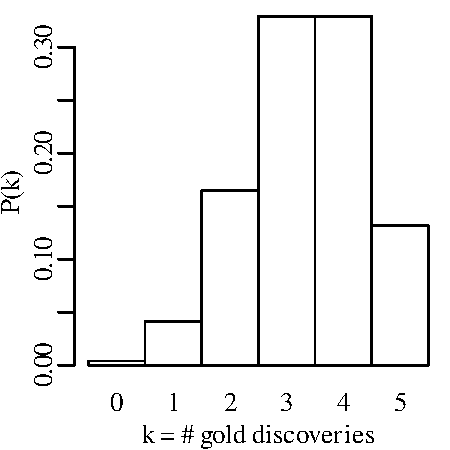
\includegraphics[width=\textwidth]{../figures/goldbarplot.pdf}
\end{minipage}
\begin{minipage}[t][][t]{.7\textwidth}
  \captionof{figure}{The probability mass function (PMF) for a
    binomial experiment with a 2/3 chance of success (and a 1/3 chance
    of failure) for five gold prospecting claims. The horizontal axis
    is labelled with the number of claims that produce gold. The
    vertical axis shows the probability of these respective outcomes.}
  \label{fig:goldbar}
\end{minipage}

The generic equation for the binomial distribution is

\begin{equation}
  P(k|n,p) = \binom{n}{k} p^k (1-p)^{n-k}
  \label{eq:binom}
\end{equation}

\noindent where $p$ is the probability of success and $k$ is the
number of successes out of $n$ trials. Equivalently, the results can
also be shown as a \textbf{cumulative distribution function} (CDF):

\begin{equation}
  F(x) = P(X \leq x)
  \label{eq:CDF}
\end{equation}

\noindent\begin{minipage}[t][][b]{.3\textwidth}
  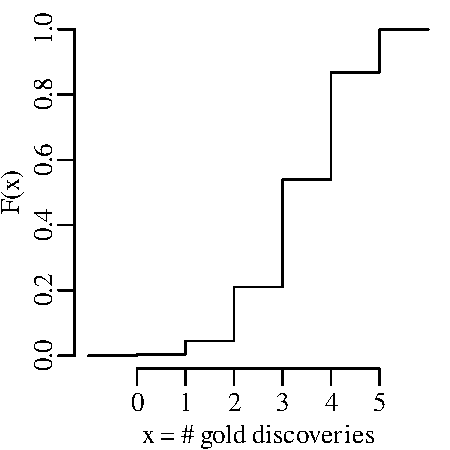
\includegraphics[width=\textwidth]{../figures/goldCDF.pdf}
\end{minipage}
\begin{minipage}[t][][t]{.7\textwidth}
  \captionof{figure}{The cumulative distribution function (CDF) of the
    binomial distribution. This is the running sum of
    Figure~\ref{fig:goldbar}. The horizontal axis is labelled with the
    number of claims that produce gold. The vertical axis shows the
    cumulative probability of these respective outcomes. For example,
    the probability that two or fewer prospectors find gold is 21\%.}
  \label{fig:goldCDF}
\end{minipage}

\section{Parameter estimation}
\label{sec:binompar}

The previous section assumed that the probability of success ($p$ in
Equation~\ref{eq:binom}) is known.  In the real world, this is rarely
the case. In fact, $p$ is usually the parameter whose value we want to
determine based on some data. Consider the general case of $k$
successes among $n$ trials. Then we can estimate $p$ by reformulating
Equation~\ref{eq:binom} in terms of $p$ instead of $k$:

\begin{equation}
  \mathcal{L}(p|n,k) = \binom{n}{k} p^k (1-p)^{n-k}
  \label{eq:Lbinom}
\end{equation}

This is called the \textbf{likelihood function}. The only difference
between the probability mass function (Equation~\ref{eq:binom}) and
the likelihood function (Equation~\ref{eq:Lbinom}) is that former
estimates the probability of an outcome given the parameter
($P(k|n,p)$), whereas the latter estimates the parameter given some
data ($P(p|n,k)$). The \emph{most likely} value of $p$ given $n$ and
$k$ can be found by taking the derivative of Equation~\ref{eq:Lbinom}
with respect to $p$ and setting it to zero:

\[
\frac{\partial{\mathcal{L}(p|n,k)}}{\partial{p}} = 0
\]

\noindent which gives

\[
  \binom{n}{k} k p^{k-1} (1-p)^{n-k} -  \binom{n}{k} p^k (n-k) (1-p)^{n-k-1} = 0
\]

Dividing by $\binom{n}{k}$ and rearranging:

\[
  k p^{k-1} (1-p)^{n-k} = p^k (n-k) (1-p)^{n-k-1}
\]

Dividing both sides by $p^k (1-p)^{n-k}$:

\[
k (1-p) = p (n-k)
\]

\noindent which can be solved for $p$:

\begin{equation}
  \hat{p} = \frac{k}{n}
  \label{eq:phat}
\end{equation}

The $\hat{~}$ symbol indicates that $\hat{p}$ is an \emph{estimate}
for $p$ that may differ from the actual parameter value $p$.\\

Let us apply Equation~\ref{eq:phat} to our gold prospecting example.
Suppose that only two of the five claims produce gold. Then our best
estimate for $p$ given this result is

\[
\hat{p} = \frac{2}{5} = 0.4
\]

So based on this very small dataset, our best estimate for the
abundance of gold in the Sierra Nevada foothills is 40\%. This may be
a trivial result, but it is nevertheless a useful one. The derivation
of Equation~\ref{eq:phat} from Equation~\ref{eq:Lbinom} follows a
recipe that underpins much of mathematical statistics. It is called
the \textbf{method of maximum likelihood}. Of course, the derivation
of parameter estimates is not always as easy as it is for the binomial
case.

\section{Hypothesis tests}
\label{sec:binomH}

Let us continue with our gold prospecting example. Given that only two
of the five prospectors found gold, our best estimate for the
abundance of gold-bearing claims in the prospecting area is $\hat{p} =
2/5$ (40\%). However the introductory paragraph to this chapter
mentioned that geological evidence suggests that 2/3 (67\%) of the
claims should contain gold. Can the discrepancy between the predicted
and the observed number of successes by attributed to bad luck, or
does it mean that the geological estimates were wrong? To answer this
question, we follow the following sequence of steps:

\begin{enumerate}

\item Formulate two hypotheses:\\

\noindent\begin{minipage}{.4\textwidth}
  $H_\circ$ (\textbf{null hypothesis})
  
  \vspace{1em}
  
  $H_a$ (\textbf{alternative hypothesis}):
\end{minipage}
\begin{minipage}{.2\textwidth}
\end{minipage}
\begin{minipage}{.2\textwidth}
  $p={2/3}$
  
  \vspace{1em}
  
  $p<{2/3}$
\end{minipage}
\begin{minipage}{.2\textwidth}
\end{minipage}\\

\item Calculate the \textbf{test statistic} $T$, which in this case is
  the number of success ($k$).

\item Determine the \textbf{null distribution} of $T$ under
  $H_\circ$. In our example this is the binomial distribution, as
  shown in Figures~\ref{fig:goldbar} and \ref{fig:goldCDF}. Tabulating
  the PMF and CDF of success:

  \begin{center}
  \begin{tabular}{ccccccc}
    k & 0 & 1 & \textit{2} & 3 & 4 & 5 \\ \hline
    $P(T=k)$ & 0.0041 & 0.0411 & \textit{0.1646} & 0.3292 & 0.3292 & 0.1317 \\
    $P({T}\leq{k})$ & 0.0041 & 0.0453 & \textit{0.2099} & 0.5391 & 0.8683 & 1.0000
  \end{tabular}
  \end{center}


The \textbf{p-value}\footnote{The term `p-value' is not to be confused
  with the value of our unknown binomial parameter $p$. The p-value
  would exist even if we had named the binomial parameter something
  else (e.g., $q$).} is the probability of obtaining test results at
least as extreme as the results actually observed, under the
assumption that the null hypothesis is correct. For our one-sided
test, the p-value is 0.2099, which corresponds the probability of
observing $k\leq{2}$ successful claims if $p=2/3$.
  
\item Choose a \textbf{significance level $\alpha$}. It is customary
  to choose $\alpha=0.05$.

\item\label{it:rejection} Mark all the outcomes that are incompatible
  with $H_\circ$.  This \textbf{rejection region} is marked in bold in
  the following table:

  \begin{center}
  \begin{tabular}{ccccccc}
    k & \textbf{0} & \textbf{1} & \textit{2} & 3 & 4 & 5 \\ \hline
    $P(T=k)$ & 0.0041 & 0.0411 & \textit{0.1646} & 0.3292 & 0.3292 & 0.1317 \\
    $P({T}\leq{k})$ & \textbf{0.0041} & \textbf{0.0453} &
    \textit{0.2099} & 0.5391 & 0.8683 & 1.0000
  \end{tabular}
  \end{center}

  $k=0$ and $k=1$ are incompatible with $H_\circ$ because the
  probability of finding gold in $k\leq{1}$ claims is only 0.0453,
  which is less than $\alpha$. Therefore our rejection region contains
  two values:
  
  \[
  R = \{0,1\}
  \]

\item\label{it:decision} Reach a \textbf{decision}. Evaluate whether
  the observed outcome for the test statistics falls inside the
  rejection region. If it does, then $H_\circ$ is rejected in favour
  of $H_a$. In our example,

  \[
  k=2\notin{R}
  \]

  \noindent which means that we cannot reject $H_\circ$.
  Alternatively, and equivalently, we can reach the same conclusion by
  observing that the p-value is greater than $\alpha$ (i.e.,
  $0.2099>0.05$). \textit{Note that failure to reject the null
    hypothesis does \underline{not} mean that said hypothesis has been
    \underline{accepted}!}\label{pag:notaccepted}
  
\end{enumerate}

Displaying the rejection region graphically:\\

\noindent\begin{minipage}[t][][b]{.6\textwidth}
  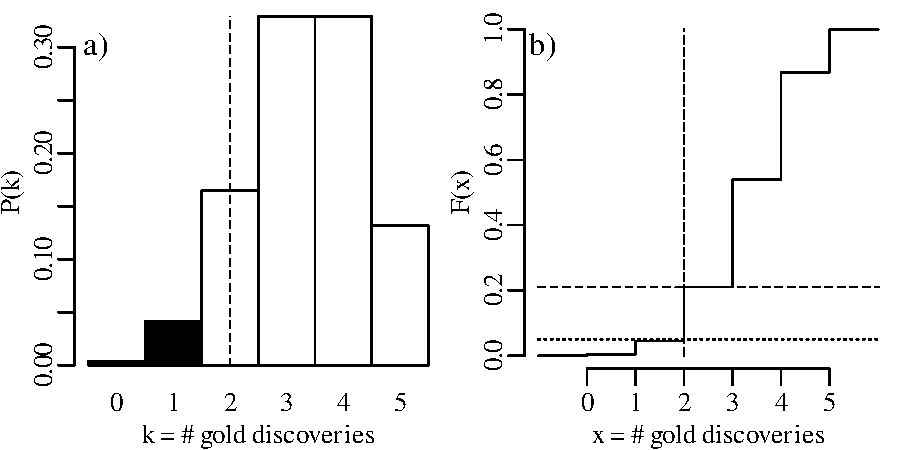
\includegraphics[width=\textwidth]{../figures/1sidedbinomialrejection5.pdf}\\
\end{minipage}
\begin{minipage}[t][][t]{.4\textwidth}
  \captionof{figure}{a) PMF and b) CDF of a binomial null distribution
    with $p=2/3$ and $n=5$. The rejection region is marked in black on
    a).  The horizontal dotted line in b) shows the $\alpha=0.05$
    cutoff mark. The horizontal dashed line in b) marks the p-value
    for $k=2$, which is greater than 0.05. Therefore, the null
    hypothesis cannot be rejected.}
  \label{fig:1sidedbinomialrejection5}
\end{minipage}

The above hypothesis test is called a \textbf{one-sided} hypothesis
test, because $H_\circ$ and $H_a$ are asymmetric.  Alternatively, we
can also formulate a \textbf{two-sided} hypothesis test:

\begin{enumerate}

\item In this case $H_\circ$ and $H_a$ are symmetric:\\

\noindent\begin{minipage}{.4\textwidth}
  $H_\circ$ (null hypothesis)
  
  \vspace{1em}
  
  $H_a$ (alternative hypothesis):
\end{minipage}
\begin{minipage}{.2\textwidth}
\end{minipage}
\begin{minipage}{.2\textwidth}
  $p=2/3$
  
  \vspace{1em}
  
  ${p}\neq{2/3}$
\end{minipage}
\begin{minipage}{.2\textwidth}
\end{minipage}\\

\item The test statistic remains the same as before.

\item We add one line to our table of cumulative outcomes, in order to
  evaluate the high end of the scale as well as its low end:

  \begin{center}
    \begin{tabular}{ccccccc}
      k & 0 & 1 & \textit{2} & 3 & 4 & 5 \\ \hline
      $P(T=k)$ & 0.0041 & 0.0411 & \textit{0.1646} & 0.3292 & 0.3292 & 0.1317 \\
      $P({T}\leq{k})$ & 0.0041 & 0.0453 & \textit{0.2099} &
      0.5391 & 0.8683 & 1.0000 \\
      $P({T}\geq{k})$ & 1.000 & 0.9959 & \textit{0.9547} &
      0.7901 & 0.4609 & 0.1317
    \end{tabular}
  \end{center}
  
\item The significance level is kept the same, but is now evaluated
  twice at $\alpha/2$ to accommodate both tails of the binomial
  distribution.

\item Mark all the outcomes that are incompatible with $H_\circ$,
  i.e. all the values $<\alpha/2$.  This \textbf{rejection region} is
  marked in bold in the following table:

  \begin{center}
    \begin{tabular}{ccccccc}
      k & \textbf{0} & 1 & \textit{2} & 3 & 4 & 5 \\ \hline
      $P(T=k)$ & 0.0041 & 0.0411 & \textit{0.1646} & 0.3292 & 0.3292 & 0.1317 \\
      $P({T}\leq{k})$ & \textbf{0.0041} & 0.0453 &
      \textit{0.2099} & 0.5391 & 0.8683 & 1.0000 \\
      $P({T}\geq{k})$ & 1.000 & 0.9959 & \textit{0.9547} & 0.7901 & 0.4609 & 0.1317
    \end{tabular}
  \end{center}

  \noindent which yields a smaller rejection region than before,
  because $P(T\leq{1})=0.0453$, which is greater than
  $\alpha/2=0.025$.  The same is true for $P(T\geq{k})$ for any
  $k$. Therefore:

  \[
  R = \{0\}
  \]

\item Again, we fail to reject $H_\circ$, which means that the
  observed $k/n=2/5$ success rate does not rule out the possibility
  that the true value of $p=2/3$, and that the geologists were
  therefore correct.
  
\end{enumerate}

Displaying the two-sided hypothesis test graphically:\\

\noindent\begin{minipage}[t][][b]{.6\textwidth}
  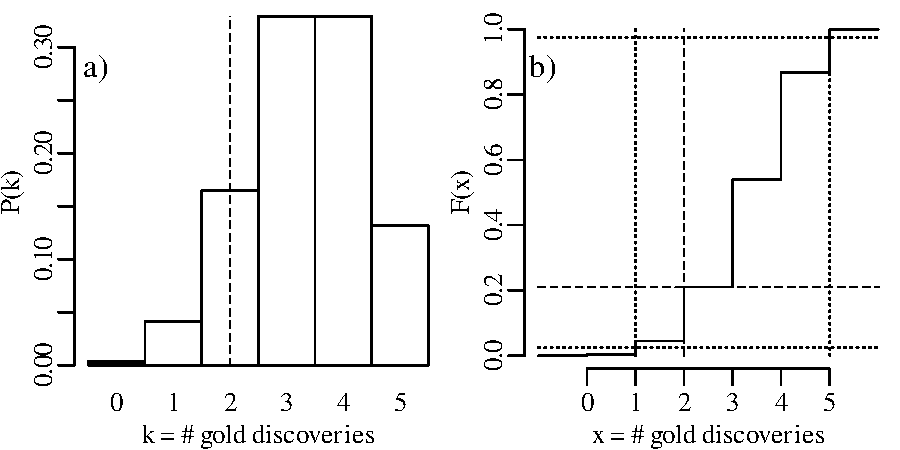
\includegraphics[width=\textwidth]{../figures/2sidedbinomialrejection5.pdf}\\
\end{minipage}
\begin{minipage}[t][][t]{.4\textwidth}
  \captionof{figure}{a) the same PMF and b) CDF as
    Figure~\ref{fig:1sidedbinomialrejection5}. The black bar marks the
    rejection region for $H_\circ: p=2/3$ vs $H_a:
    p\neq{2/3}$. Horizontal dotted lines mark $\alpha/2=0.025$ and
    $(1-\alpha/2)=0.975$. Their intersections with the CDF are shown
    as vertical dotted lines and mark the outer edges of the rejection
    region.  The dashed lines mark the observed value and probability,
    which fall outside the rejection region. Therefore $H_\circ$
    stands.}
  \label{fig:2sidedbinomialrejection5}
\end{minipage}

So in this case the one-sided and two-sided hypothesis tests produce
exactly the same result. However this is not always the case.

\section{Statistical power}
\label{sec:power}

Suppose that not five but fifteen gold prospectors had purchased a
claim in the same area as before. And suppose that six of these
prospectors had struck gold. Then the maximum likelihood estimate for
$p$ is:

\[
\hat{p} = \frac{6}{15} = 0.4
\]

\noindent which is the same as before. The one-sided hypothesis test
($H_\circ: p={2/3}$ vs. $H_a: p<2/3$) proceeds as before, but leads to
a different table of probabilities:

\begin{center}
  \begin{tabular}{c@{\gap}c@{\gap}c@{\gap}c@{\gap}c@{\gap}c@{\gap}c@{\gap}c@{\gap}c}
    k & \textbf{0} & \textbf{1} & \textbf{2} & \textbf{3} & \textbf{4}
    & \textbf{5} & \textbf{\textit{6}} & 7 \\ \hline $P(T=k)$ &
    7.0$\times{10}^{-8}$ & 2.1$\times{10}^{-6}$ & 2.9$\times{10}^{-5}$
    & 2.5$\times{10}^{-4}$ & 0.0015 & 0.0067 & \textit{0.0223} & 0.0574 \\
    $P({T}\leq{k})$ & \textbf{7.0}$\mathbf{\times{10}^{-8}}$
    & \textbf{2.2}$\mathbf{\times{10}^{-6}}$ &
    \textbf{3.1}$\mathbf{\times{10}^{-5}}$ &
    \textbf{2.8}$\mathbf{\times{10}^{-4}}$ & \textbf{0.0018} &
    \textbf{0.0085} & \textbf{\textit{0.0308}} & 0.0882 \\
    k & 8 & 9 & 10 & 11 & 12 & 13 & 14 & 15 \\
    \hline $P(T=k)$ & 0.1148 & 0.1786 & 0.2143
    & 0.1948 & 0.1299 & 0.0599 & 0.0171 & 0.0023 \\
    $P({T}\leq{k})$ & 0.2030 & 0.3816 & 0.5959 & 0.7908 &
    0.9206 & 0.9806 & 0.9977 & 1.0000 \\
  \end{tabular}
\end{center}

The rejection region (bold) consists of

\begin{equation}
  R=\{0,1,2,3,4,5,6\}
  \label{eq:1sidedbinomtest15}
\end{equation}

\noindent which includes $k=6$. Therefore $H_\circ$ has been rejected.

\noindent\begin{minipage}[t][][b]{.6\textwidth}
  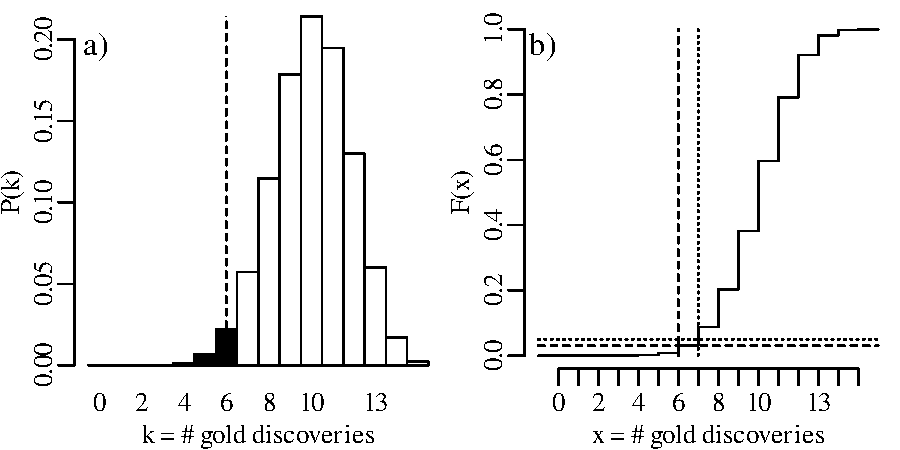
\includegraphics[width=\textwidth]{../figures/1sidedbinomialrejection15.pdf}\\
\end{minipage}
\begin{minipage}[t][][t]{.4\textwidth}
  \captionof{figure}{a) PMF and b) CDF of a binomial distribution with
    $p={2/3}$ and $n=15$. The $\alpha=0.05$ cutoff is shown as a
    horizontal dotted line and intersects the CDF at a point marked by
    a vertical dotted line. The vertical dashed lines mark the
    observation ($k=6$), which falls in the black area of the bar
    chart, and to the left of the dotted line in the CDF. Therefore,
    $H_\circ$ is rejected.}
  \label{fig:1sidedbinomialrejection15}
\end{minipage}

For the two-sided hypothesis test ($H_\circ: p={2/3}$ vs. $H_a:
p\neq{2/3}$):

\begin{center}
\begin{tabular}{c@{\gap}c@{\gap}c@{\gap}c@{\gap}c@{\gap}c@{\gap}c@{\gap}c@{\gap}c}
    k & \textbf{0} & \textbf{1} & \textbf{2} & \textbf{3} & \textbf{4}
    & \textbf{5} & \textit{6} & 7 \\ \hline $P(T=k)$ &
    7.0$\times{10}^{-8}$ & 2.1$\times{10}^{-6}$ & 2.9$\times{10}^{-5}$
    & 2.5$\times{10}^{-4}$ & 0.0015 & 0.0067 & \textit{0.0223} & 0.0574 \\
    $P({T}\leq{k})$ & \textbf{7.0}$\mathbf{\times{10}^{-8}}$ &
    \textbf{2.2}$\mathbf{\times{10}^{-6}}$ &
    \textbf{3.1}$\mathbf{\times{10}^{-5}}$ &
    \textbf{2.8}$\mathbf{\times{10}^{-4}}$ & \textbf{0.0018} &
    \textbf{0.0085} & \textit{0.0308} & 0.0882 \\
    $P({T}\geq{k})$ & 1.0000 &
    1-7.0$\times{10}^{-8}$ & 1-2.2$\times{10}^{-6}$ &
    1-3.1$\times{10}^{-5}$ & 1-2.8$\times{10}^{-4}$ & 0.9982 & \textit{0.9915}
    & 0.9692 \\ k & 8 & 9 & 10 & 11 & 12 & 13 & \textbf{14} & \textbf{15} \\ \hline
    $P(T=k)$ & 0.1148 & 0.1786 & 0.2143 & 0.1948
    & 0.1299 & 0.0599 & 0.0171 & 0.0023 \\
    $P({T}\leq{k})$ & 0.2030 &
    0.3816 & 0.5959 & 0.7908 & 0.9206 & 0.9806 & 0.9977 & 1.0000 \\
    $P({T}\geq{k})$ & 0.9118 & 0.7970 & 0.6184 & 0.4041 & 0.2092 &
    0.0794 & \textbf{0.0194} & \textbf{0.0023}
\end{tabular}
\end{center}

The rejection region (which includes both tails of the distribution)
is:

\begin{equation}
  R=\{0,1,2,3,4,5,14,15\}
  \label{eq:2sidedbinomtest15}
\end{equation}

This region does \emph{not} include $k=6$. Therefore we \emph{cannot}
reject the two-sided null hypothesis that $p=2/3$.\\

\noindent\begin{minipage}[t][][b]{.6\textwidth}
  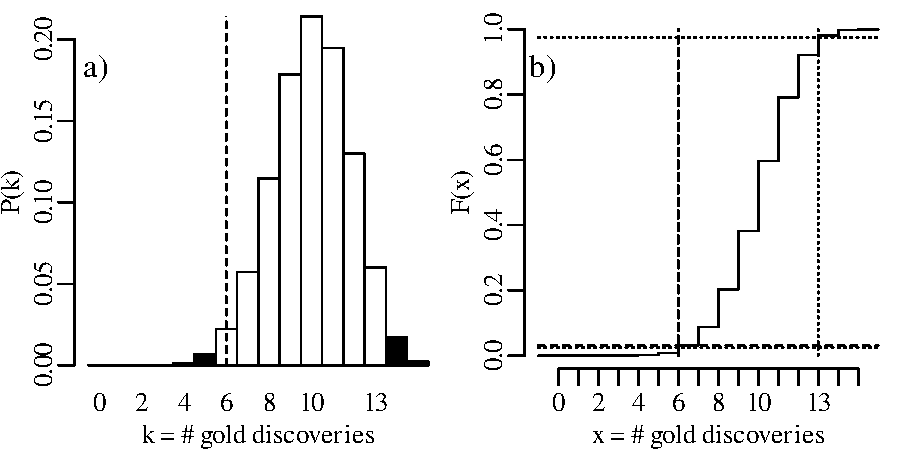
\includegraphics[width=\textwidth]{../figures/2sidedbinomialrejection15.pdf}\\
\end{minipage}
\begin{minipage}[t][][t]{.4\textwidth}
  \captionof{figure}{a) PMF and b) CDF of the binomial distribution
    with $p=2/3$ and $n=15$.  The dotted lines mark the
    $\alpha/2=0.025$ and $(1-\alpha/2)=0.975$ levels and
    quantiles. The dashed lines mark the observed value ($k=6$), which
    falls outside the rejection region.  Therefore $H_\circ$ stands.}
  \label{fig:2sidedbinomialrejection15}
\end{minipage}

Let us increase our `sample size' (number of prospectors) even more,
from 15 to 30, and suppose once again that only 40\% of these found
gold even though the geological evidence suggested that this should be
67\%. The lookup table of probabilities would be quite large, so we
will just show the distributions graphically:\\

\noindent\begin{minipage}[t][][b]{.65\textwidth}
  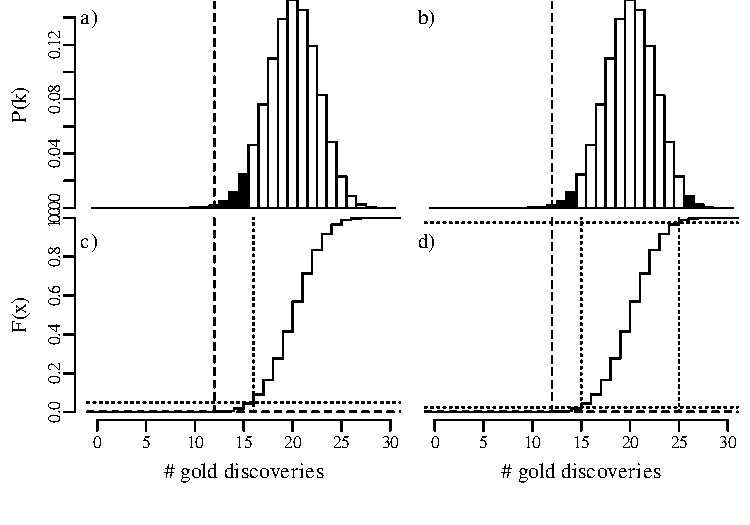
\includegraphics[width=\textwidth]{../figures/binomialrejection30.pdf}
\end{minipage}
\begin{minipage}[t][][t]{.35\textwidth}
  \captionof{figure}{The PMF (a \& b) and CDF (c \& d) for a binomial
    distribution with $p=2/3$ and $n=30$. The vertical dashed lines
    mark the observation $k=12$, which falls outside the cutoff limits
    defined by the vertical dotted lines, and inside the rejection
    regions marked in black.}
  \label{fig:binomialrejection30}
\end{minipage}

In summary, we have compared the same outcome of 40\% successes based
on three different sample sizes ($n$):

\begin{enumerate}
  \item Both the one-sided and the two-sided hypothesis tests failed
    to reject the null hypothesis for $n=5$ prospectors.
  \item Increasing the number of prospectors to $n=15$ leads to a
    rejection of $H_\circ$ in the one-sided case but failure to reject
    $H_\circ$ in the two-sided test.
  \item Further increasing our sample size to $n=30$ whilst still
    keeping the percentage of success the same leads to a firm
    rejection of both the one-sided and the two-sided null hypotheses.
\end{enumerate}

In statistical terms, the increase in sample size has increased the
`power' of the test to reject the hypothesis test. A formal
mathemathical definition of this concept will be given in
Section~\ref{sec:typeI&II}.

\section{Type-I and type-II errors}
\label{sec:typeI&II}

There are four possible outcomes for a hypothesis test, which can be
organised in a ${2}\times{2}$ table:

\begin{center}
\begin{tabular}{c|cc}
  $H_\circ$ is ... & false & true \\ \hline
  rejected & correct decision & Type-I error \\
  not rejected & Type-II error & correct decision
\end{tabular}
\end{center}

To appreciate the difference between the two types of errors in this
table, it may be useful to compare statistical hypothesis testing with
a legal analogue. The jury in a court of justice faces a situation
that is similar to that of a statistical hypothesis test. They are
faced with a criminal who has either committed a crime or not, and
they must decide whether to sentence this person or acquit them.  In
this case our `null hypothesis' is that the accused is innocent.  The
jury then needs decide whether there is enough evidence to reject this
hypothesis in favour of the alternative hypothesis, which is that the
accused in guilty. Casting this process in a second ${2}\times{2}$
table:

\begin{center}
\begin{tabular}{c|cc}
  the accused is ... & guilty & innocent \\ \hline
  sentenced & correct decision & Type-I error \\
  acquitted & Type-II error & correct decision
\end{tabular}
\end{center}

A \textbf{type-I error} is committed when a true null hypothesis test
is erroneously rejected. This is akin to putting an innocent person in
prison. For our gold prospecting example, this means that we reject
the expert opinion of the geologist (whose assessment indicated a 2/3
chance of finding gold) when this geologist is in fact correct.\\

A \textbf{type-II error} is committed when we fail to reject a false
null hypothesis.  This is akin to letting a guilty person get away
with a crime for lack of evidence. In the geological example, this
means that we still trust the geological assessment despite it being
wrong.\\

The probability of committing a type-I error is controlled by one
parameter:

\begin{enumerate}
\item {\bf The confidence level $\alpha$}
  
  Using the customary value of $\alpha=0.05$, there is a 5\% chance of
  committing a type-I error. So even if the null hypothesis is
  correct, then we would still expect to reject it once every 20
  times. This may be acceptable in geological studies, but probably
  not in the legal system! The principle that guilt must be proven
  ``beyond any reasonable doubt''is akin to choosing a very small
  significance level ($\alpha\ll{0.05}$). However it is never possible
  to enforce $\alpha=0$, so it is inevitable that some innocent people
  are sentenced.
\end{enumerate}

The probability of committing a type-II error ($\beta$) depends on two
things:

\begin{enumerate}
\item{\bf The degree to which $H_\circ$ is false}
  
  In our geological example, 40\% of the prospectors found gold in
  their claim, so there clearly was some gold present in the
  area. Suppose that the actual abundance of gold in the prospecting
  area was indeed 40\% ($p=2/5$) instead of $p=2/3$.  Then the
  expected distribution of outcomes would follow a binomial
  distribution with $p=2/5$. As shown in Section~\ref{sec:binomH}, the
  rejection region for the one-sided hypothesis test of $H_\circ:
  p=2/3$ vs. $H_a: p<2/3$ is $R=\{0\}$. If the actual value for $p$ is
  2/5, then the probability a value for $k$ that falls in this
  rejection region is $P(k<2|n=5,p=2/5)=0.34$. This is known as the
  \textbf{power} of the statistical test. The probability of
  committing a type-II error is given by:
  
  \begin{equation}
    \beta = 1 - \mbox{power} = 0.66
  \end{equation}

  Next, suppose that the true probability of finding gold is even
  lower, at $p=1/5$. Under this alternative distribution, the
  probability of finding gold in ${k}\leq{1}$ claims (and, hence, the
  power) increases to 74\%. Therefore, the probability of committing a
  type-II error has dropped to only 26\%.

  Finally, consider an end member situation in which the prospecting
  area does not contain any gold at all ($p=0$). Then the probability
  of finding gold is obviously zero ($F(x=2)=0$). Under this trivial
  scenario, the power of the test is 100\%, and the probability of
  committing a type-II error is zero.

  Plotting these results graphically:

  \noindent\begin{minipage}[t][][b]{\indentwidth}
    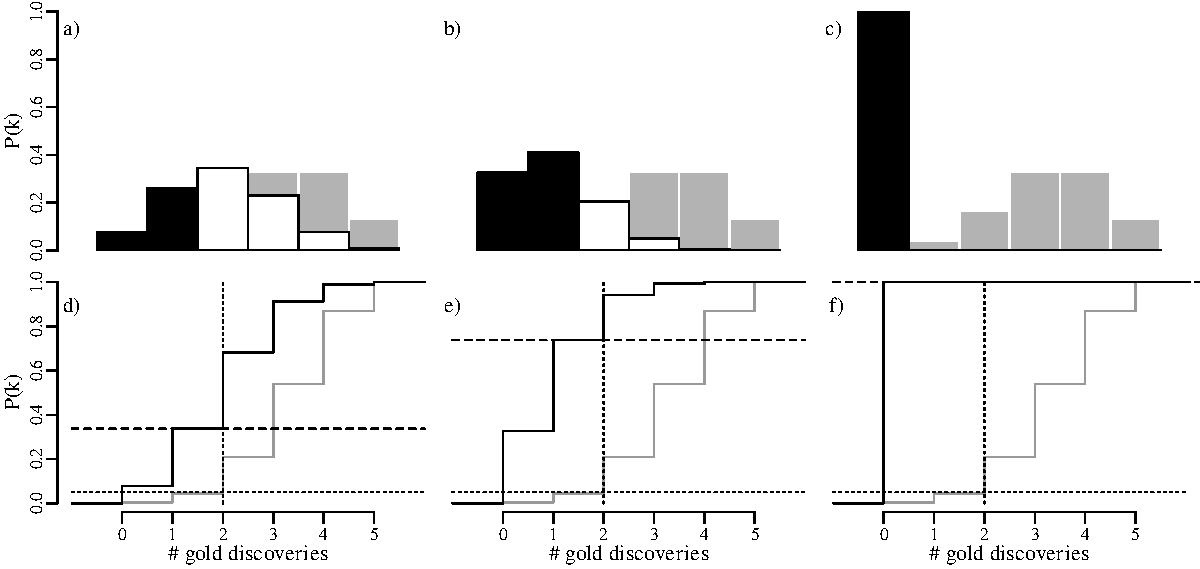
\includegraphics[width=\textwidth]{../figures/binompower1.pdf}
  \end{minipage}
  \begin{minipage}[t][][t]{\indentwidth}
  \captionof{figure}{a) -- c) PMFs of the binomial null distribution
    with $p=2/3$ ($H_\circ$, grey) and alternative distributions with
    a) $p=2/5$, b) $p=1/5$ and c) $p=0$. Sample size is $n=5$ for all
    cases.  d) -- f) CDFs for the null distribution (grey) and the
    alternative distribution (black). The horizontal dotted lines mark
    $\alpha=0.05$.  Their intersections with the CDF of the null
    distribution are marked by vertical dotted lines. The areas to the
    left of these lines define the rejection region and are marked in
    black in the bar chart. The larger the sample size, the easier it
    is to reject $H_\circ$. The dashed horizontal lines mark the
    intersection of the rejection region with the CDF of the
    alternative distribution. These mark the power of the statistical
    test ($1-\beta$).  Power clearly increases as the alternative
    distribution drifts away from the null distribution.}
  \label{fig:binompower1}
  \end{minipage}

\item{\bf Sample size}

  The effect of sample size was already discussed in section
  \ref{sec:power}. Comparing the predicted outcomes for the null
  hypothesis $H_\circ: p=2/3$ to those of the alternative hypothesis
  $H_a: p=2/5$ for sample sizes of $n=5$, 15 and 30:

  \begin{minipage}[t][][b]{\indentwidth}
    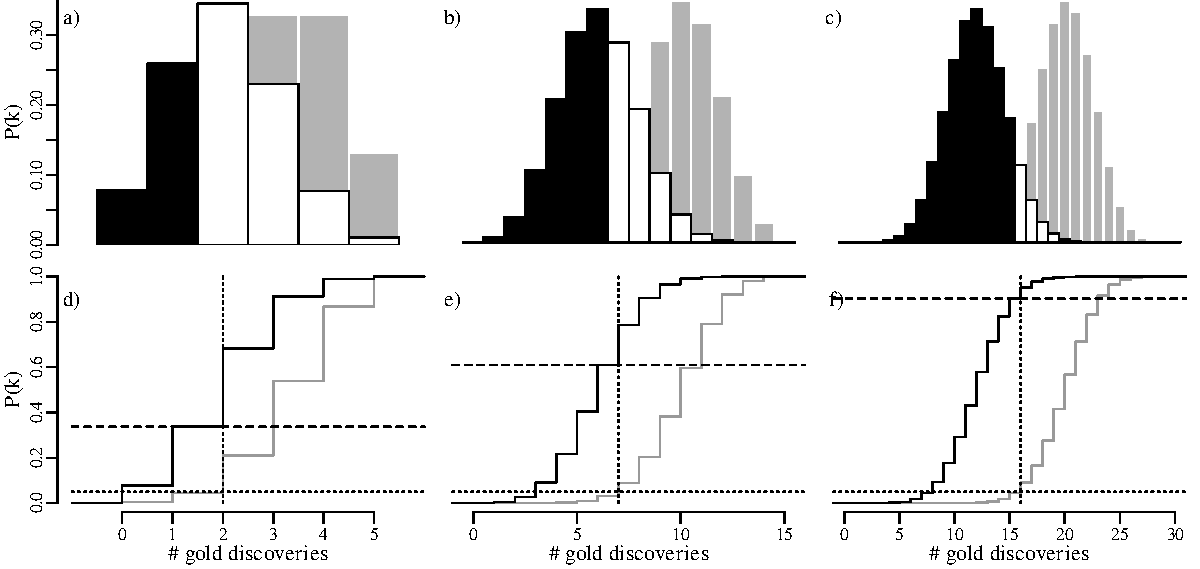
\includegraphics[width=\textwidth]{../figures/binompower2.pdf}
  \end{minipage}
  \begin{minipage}[t][][t]{\indentwidth}
    \captionof{figure}{a) -- c) PMFs of binomial distributions with
      $p=2/3$ ($H_\circ$, grey) and $p=2/5$ ($H_a$, black and white),
      for sample sizes of a) $n=5$, b) $n=15$ and c) $n=30$.  d) -- f)
      CDFs for the null distribution (grey) and the alternative
      distribution (black). The horizontal dotted lines mark
      $\alpha=0.05$.  Their intersections with the CDF of the null
      distribution are marked by vertical dotted lines. The area to
      the left of these lines define the rejection region and are
      marked in black in the bar chart. The larger the sample size,
      the easier it is to reject $H_\circ$. The dashed horizontal
      lines mark the intersection of the rejection region with the CDF
      of the alternative distribution. These mark the power of the
      statistical test ($1-\beta$).  Power clearly increases with
      sample size.}
    \label{fig:binompower2}
  \end{minipage}

\end{enumerate}

\section{Pitfalls of statistical hypothesis testing}
\label{sec:pitfalls}

\hspace{\parindent}\textit{All hypotheses are wrong ... in some decimal place}
\hfill-- John Tukey (paraphrased)\\

\textit{All models are wrong, but some are useful}
\hfill-- George Box\\

Statistical tests provide a rigorous mathematical framework to assess
the validity of a hypothesis. It is not difficult to see the appeal of
this approach to scientists, including geologists. The scientific
method is based on three simple steps:

\begin{enumerate}
\item Formulate a hypothesis.
\item Design an experiment to test said hypothesis.
\item Carry out the experiment and check to see if it matches the prediction.
\end{enumerate}

It is rarely possible to prove scientific hypotheses. We can only
\emph{disprove} them. New knowledge is gained when the results of an
experiment do not match the expectations. For example:

\begin{enumerate}
\item Hypothesis: Earth's lower mantle is made of olivine.
\item Test: Study the stability of olivine at lower mantle pressures
  (24-136~GPa).
\item Result: Olivine is not stable at lower mantle pressures.
\end{enumerate}

From this experiment we still don't know what the lower mantle is made
of.  But at least we know that it is \emph{not} olivine. Let us
contrast this outcome with a second type of hypothesis:

\begin{enumerate}
\item Hypothesis: Earth's lower mantle is made of perovskite.
\item Test: Study the stability of perovskite at lower mantle
  pressures.
\item Result: Perovskite is stable at lower mantle pressures.
\end{enumerate}

What have we learned from this experiment? Not much. We certainly did
not prove that Earth's lower mantle consists of perovskite. There are
lots of other minerals that are stable at lower mantle pressures. The
only thing that we can say is that the null hypothesis has survived to
live another day. The scientific method is strikingly similar to the
way in which a statistical hypothesis test is carried out. A null
hypothesis, like a scientific hypothesis, cannot be proven. It can
only be disproved. Rejection of a null hypothesis is the best outcome,
because it is the only outcome that teaches us something new.\\

It may seem natural to use the statistical approach to test scientific
hypotheses. However doing so is not without dangers. To explain these
dangers, let us go back to the power analysis of
Section~\ref{sec:power}. The power of our hypothesis test to reject
$H_\circ: p=2/3$ increases with sample size. A small sample may be
sufficient to detect large deviations from the null
hypothesis. Smaller deviations require larger sample sizes. But no
matter how small the violation of the null hypothesis is, there always
exists a sample size that is large enough to detect it.\\

Statistical tests are an effective way to evaluate mathematical
hypotheses. They are less useful for scientific hypotheses.  There is
a profound difference between mathematical and scientific
hypotheses. Whereas a mathematical hypothesis is either `right' or
`wrong', scientific hypotheses are always `somewhat wrong'.
Considering our gold prospecting example, it would be unreasonable to
expect that $p$ is exactly equal to 2/3, down to the
100\textsuperscript{th} significant digit.  Estimating the correct
proportion of gold in the area to better than 10\% would already be a
remarkable achievement. Yet given enough data, there will always come
a point where the geological prediction is disproved. Given a large
enough dataset, even a 1\% deviation from the predicted value would be
yield an unacceptably small p-value:

\noindent\begin{minipage}[t][][b]{.45\textwidth}
  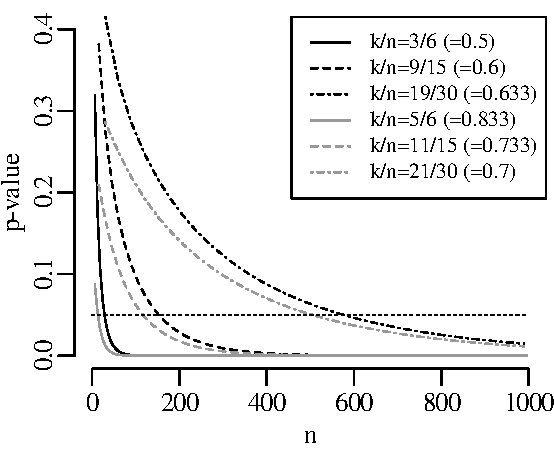
\includegraphics[width=\textwidth]{../figures/binompvsn.pdf}
\end{minipage}
\begin{minipage}[t][][t]{.55\textwidth}
  \captionof{figure}{The most likely outcome of a binomial experiment
    with $p=2/3$ is $k/n=2/3(=0.67)$. This figure shows the p-values
    of six slightly different outcomes for a range of different sample
    sizes.  The horizontal dotted line marks the 5\% significance
    level. No matter how little the observed $k/n$-ratio differs from
    2/3, this difference always becomes `significant' given a large
    enough sample size.}
  \label{fig:binomnvsp}
\end{minipage}

As another example, suppose that we have analysed the mineralogical
composition of two samples of sand that were collected 10cm apart on
the same beach. Our null hypothesis is that the composition of the two
samples is the same. Plausible though this hypothesis may seem, it
will always be possible to reject it, given a large enough
sample. Perhaps we need to classify a million grains from each sample,
but at some point a `statistically significant' difference will be
found. Given a large enough sample, even the tiniest hydraulic sorting
effect becomes detectable.\\

In conclusion, formalised hypothesis tests are of limited use in
science.  There are just two exceptions in which they do serve a
useful purpose:

\begin{enumerate}
\item If a statistical test fails to reject the null hypothesis, then
  this indicates that the sample size is too small to find a
  meaningful effect. In this context the statistical test protects
  us against over-interpreting our data.
\item We can calculate the sample size that would be required to
  detect a pre-specified deviation from the null hypothesis.  This
  approach is used in the pharmaceutical industry to test the efficacy
  of drugs. However this approach is seldom or never available to
  geologists.
\end{enumerate}

\section{Confidence intervals}
\label{sec:binomCI}

The previous section showed that simple binary hypothesis tests are of
limited use in geology. The question that is relevant to scientists is
not so much whether a hypothesis is wrong, but rather \emph{how wrong}
it is. In the context of our gold prospecting example, there is little
use in testing whether $p$ is exactly equal to $2/3$. In reality, $p$
is \emph{unknown}. It is far more useful to actually estimate $p$ and
to quantify the statistical uncertainty associated with it.\\

Equation~\ref{eq:phat} showed that, given $k$ successful claims among
$n$ total claims, the \emph{most likely} estimate for $p$ is $k/n$.
For example, if we observe $k=2$ successful claims among $n=5$ trials,
then our best estimate for the abundance of gold is $\hat{p}=2/5$.
However this does not rule out other values. Let us now explore all
possible values for $p$ that are compatible with the observed $k=2$
successful claims:

\begin{enumerate}
\item{\bf p=0?} If $p=0$, then the outcome that $k=2$ would be
  impossible.  So $p=0$ can be ruled out.
\item{\bf p=0.1?} The probability of observing ${k}\geq{2}$ successful
  claims if $p=0.1$ is given by:
  
  \[
  P({k}\geq{2}|p=0.1,n=5) =
  \sum\limits_{i=2}^{5}\binom{5}{i}(0.1)^i(0.9)^{n-i} = 0.081
  \]
  
  which is greater than $\alpha/2$. Consequently, the observation
  $k=2$ falls outside the rejection region of the two-sided hypothesis
  test, and the proposed parameter value $p=0.1$ is deemed compatible
  with the observation.
\item{\bf p=2/5?} This is our maximum likelihood estimate for $p$.  It
  is definitely possible that this is the true value.
\item{\bf p=2/3?} Figures~\ref{fig:binompower1}.b) and e) show that
  there is a greater than 5\% chance of observing 2 or fewer
  successful claims if the true value of $p$ is $2/3$. So $p=2/3$
  remains possible.
\item{\bf p=0.9?} The probability of observing ${k}\leq{2}$ successful
  claims if $p=0.9$ is given by:
  \[
  P({k}\leq{2}|p=0.9,n=5) =
  \sum\limits_{i=0}^{2}\binom{5}{i}(0.9)^i(0.1)^{n-i} = 0.0086
  \]
  which is less than the $\alpha/2$ cutoff, and so $p=0.9$ is
  \emph{not} compatible with the observation.
\item{\bf p=1?} If $p=1$, then 100\% of the claims should contain
  gold. This is incompatible with the observation that $k=2$.
  Therefore $p=1$ can be ruled out.
\end{enumerate}

The set of all values of $p$ that are compatible with the observed
outcome $k=2$ forms a \textbf{confidence interval}. Using an iterative
process, it can be shown that the lower and upper limits of this
interval are given by:

\[
\mbox{C.I.}(p|k=2,n=5) = [0.053, 0.85]
\]

\noindent\begin{minipage}[t][][b]{.65\textwidth}
  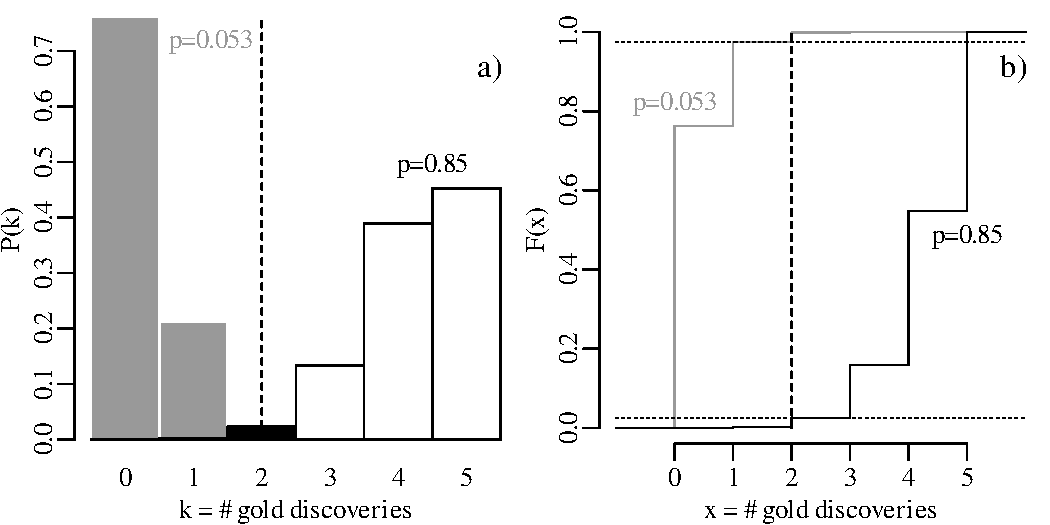
\includegraphics[width=\textwidth]{../figures/binomcik2n5.pdf}\\
\end{minipage}
\begin{minipage}[t][][t]{.35\textwidth}
  \captionof{figure}{95\% confidence interval for the binomial
    parameter $p$ given $k=2$ successful claims (dashed lines) out of
    $n=5$.  The lower ($p=0.053$, grey) and upper ($p=0.85$) limits of
    the confidence interval are shown as a) PMFs and b) CDFs. Dotted
    horizontal lines mark the 0.025 and 0.975 confidence levels.\\}
  \label{fig:binomcik2n5}
\end{minipage}

Repeating this procedure for a different result, for example $k=4$,
yields a different confidence interval, namely:

\[
\mbox{C.I.}(p|k=4,n=5) = [0.284, 0.995]
\]

\noindent\begin{minipage}[t][][b]{.65\textwidth}
  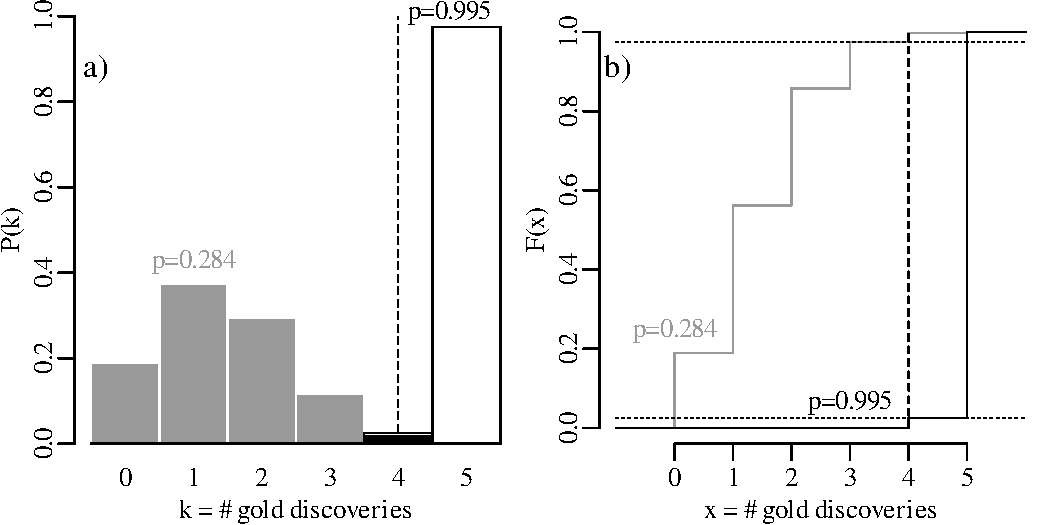
\includegraphics[width=\textwidth]{../figures/binomcik4n5.pdf}\\
\end{minipage}
\begin{minipage}[t][][t]{.35\textwidth}
  \captionof{figure}{95\% confidence interval for the binomial
    parameter $p$ given $k=4$ successful claims (dashed lines) out of
    $n=5$ trials.  The lower ($p=0.284$, grey) and upper ($p=0.995$)
    limits of the confidence interval are shown as a) PMFs and b)
    CDFs. Dotted horizontal lines mark the 0.025 and 0.975 confidence
    levels.\\}
  \label{fig:binomcik4n5}
\end{minipage}

What happens if we increase the sample size from $n=5$ to $n=30$, and
the number of successful claims from $k=2$ to $k=12$?  Then the
maximum likelihood estimate remains $\hat{p}=2/5$ as in our first
example, but the 95\% confidence interval narrows down to

\[
\mbox{C.I.}(p|k=12,n=30) = [0.23, 0.59]
\]

\noindent\begin{minipage}[t][][b]{.65\textwidth}
  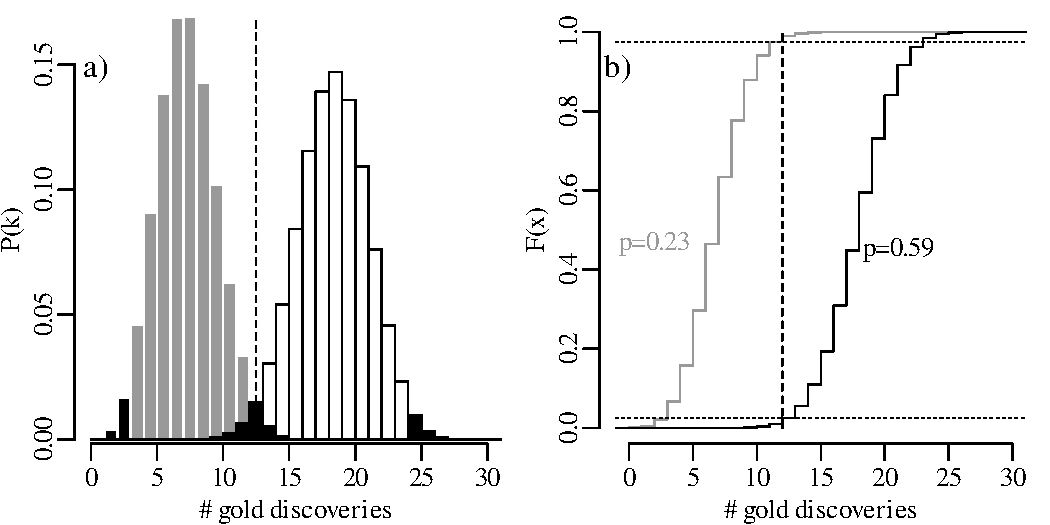
\includegraphics[width=\textwidth]{../figures/binomcik12n30.pdf}\\
\end{minipage}
\begin{minipage}[t][][t]{.35\textwidth}
  \captionof{figure}{95\% confidence interval for the binomial
    parameter $p$ given $k=12$ successful claims (dashed lines) out of
    $n=30$ trials.  The lower ($p=0.23$, grey) and upper ($p=0.59$)
    limits of the confidence interval are shown as a) PMFs and b)
    CDFs. Dotted horizontal lines mark the 0.025 and 0.975 confidence
    levels.\\}
  \label{fig:binomcik12n30}
\end{minipage}

To further explore the trend of decreasing confidence interval width
with increasing sample size, let us evaluate the 95\% confidence
intervals for $\hat{p}=k/n$ estimates of 2/3 and 1/5, respectively,
over a range of sample sizes between $n=3$ and $n=300$:\\

\noindent\begin{minipage}[t][][b]{.65\textwidth}
  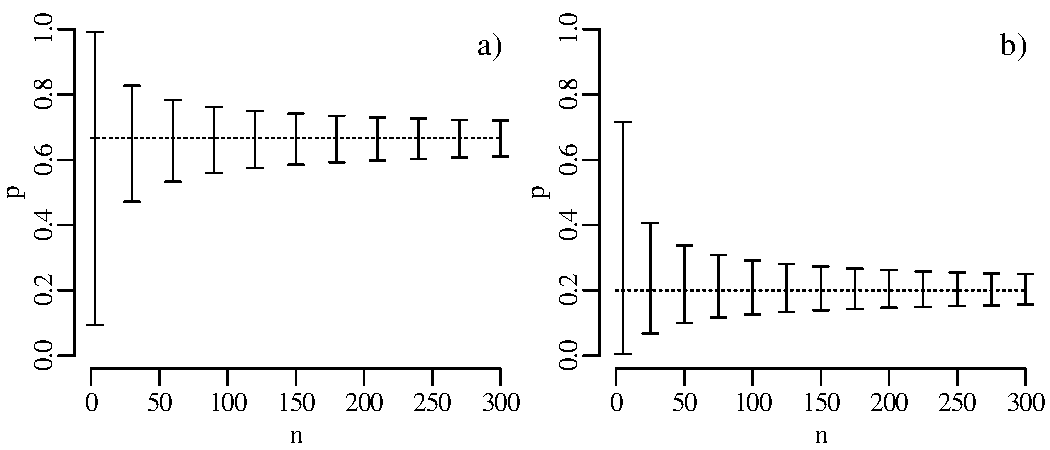
\includegraphics[width=\textwidth]{../figures/binomcivsn.pdf}\\
\end{minipage}
\begin{minipage}[t][][t]{.35\textwidth}
  \captionof{figure}{95\% confidence intervals for a) $\hat{p}=2/3$
    and b) $\hat{p}=1/5$ for different sample sizes $n$. The
    horizontal dotted lines mark the maximum likelihood
    estimates. Note the asymmetry of the confidence intervals, which
    always fall within the 0 to 1 range of the parameter.}
  \label{fig:binomcivsn}
\end{minipage}

The confidence intervals become progressively narrower with increasing
sample size. This reflects a steady improvement of the
\textbf{precision} of our estimate for $p$ with increasing sample
size. In other words, large datasets are `rewarded' with better
precision.


\chapter{The Poisson distribution}
\label{ch:poisson}

\textbf{\underline{Example~1}}\medskip

A \emph{declustered} earthquake catalog\footnote{Mueller, C.S.,
  2019. Earthquake catalogs for the USGS national seismic hazard
  maps. \textit{Seismological Research Letters}, 90(1), pp.251-261.}
of the western United States contains 543 events of magnitude 5.0 and
greater that occurred between 1917 and 2016:\medskip

\noindent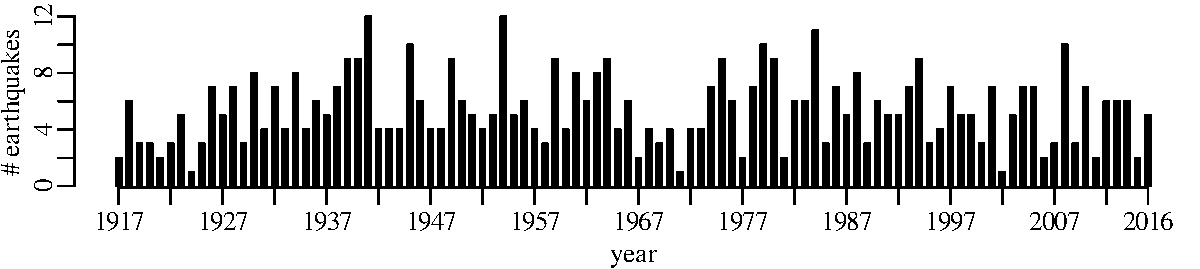
\includegraphics[width=\textwidth]{../figures/declusteredquakes.pdf}
\begingroup \captionof{figure}{The number of US earthquakes of
  magnitude 5.0 or greater per year between 1917 and 2016, with
  aftershocks removed.\medskip}
\label{fig:declusteredquakes}
\endgroup

The number of earthquakes in each bin forms a new dataset of 100
numbers, which has the following summary statistics:

\noindent\begin{minipage}[t][][b]{.4\textwidth}
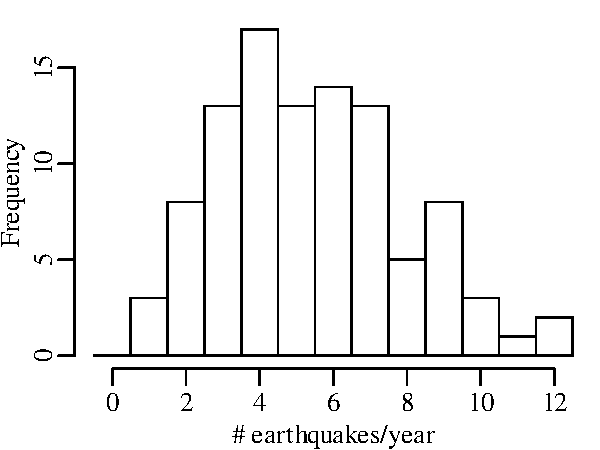
\includegraphics[width=\textwidth]{../figures/declusteredquakesperyear.pdf}
\medskip
\end{minipage}
\begin{minipage}[t][][t]{.6\textwidth}
  \captionof{figure}{ Histogram of the earthquake counts shown in
    Figure~\ref{fig:declusteredquakes}.\medskip
    ~\\
    \textbf{mean: 5.43}\\
    standard deviation: 2.50\\
    \textbf{variance: 6.24}
  }
  \label{fig:declusteredquakesperyear}
\end{minipage}

Note how the mean and the variance of this dataset are similar.\medskip

\noindent\textbf{\underline{Example~2}}\medskip

5000 grains of sand have been mounted in an uncovered thin section and
imaged with a scanning electron microscope (SEM). The SEM has
identified the locations of zircon (ZrSiO\textsubscript{4}) crystals
that are suitable for geochronological dating:

\noindent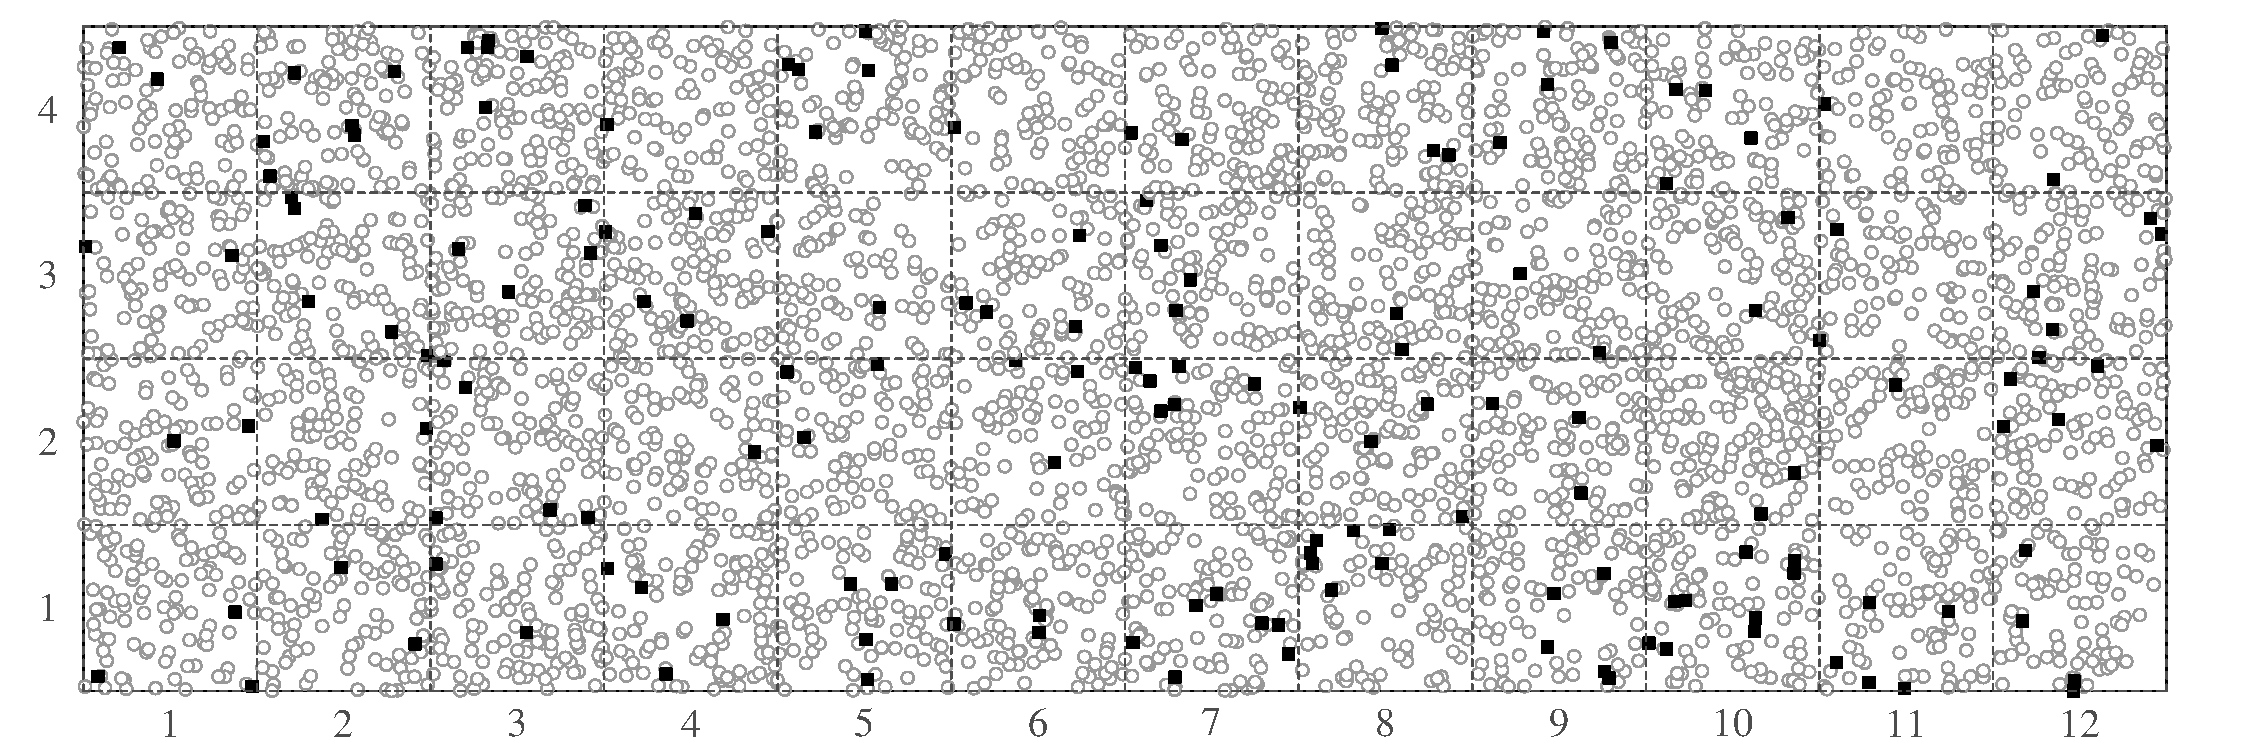
\includegraphics[width=\textwidth]{../figures/zircons.pdf}
\begingroup \captionof{figure}{Point-counting results for zircon in
  sand. Black squares mark zircons and grey circles other minerals.\medskip}
\label{fig:zircons}
\endgroup

Counting the number of zircons in the graticule:

\noindent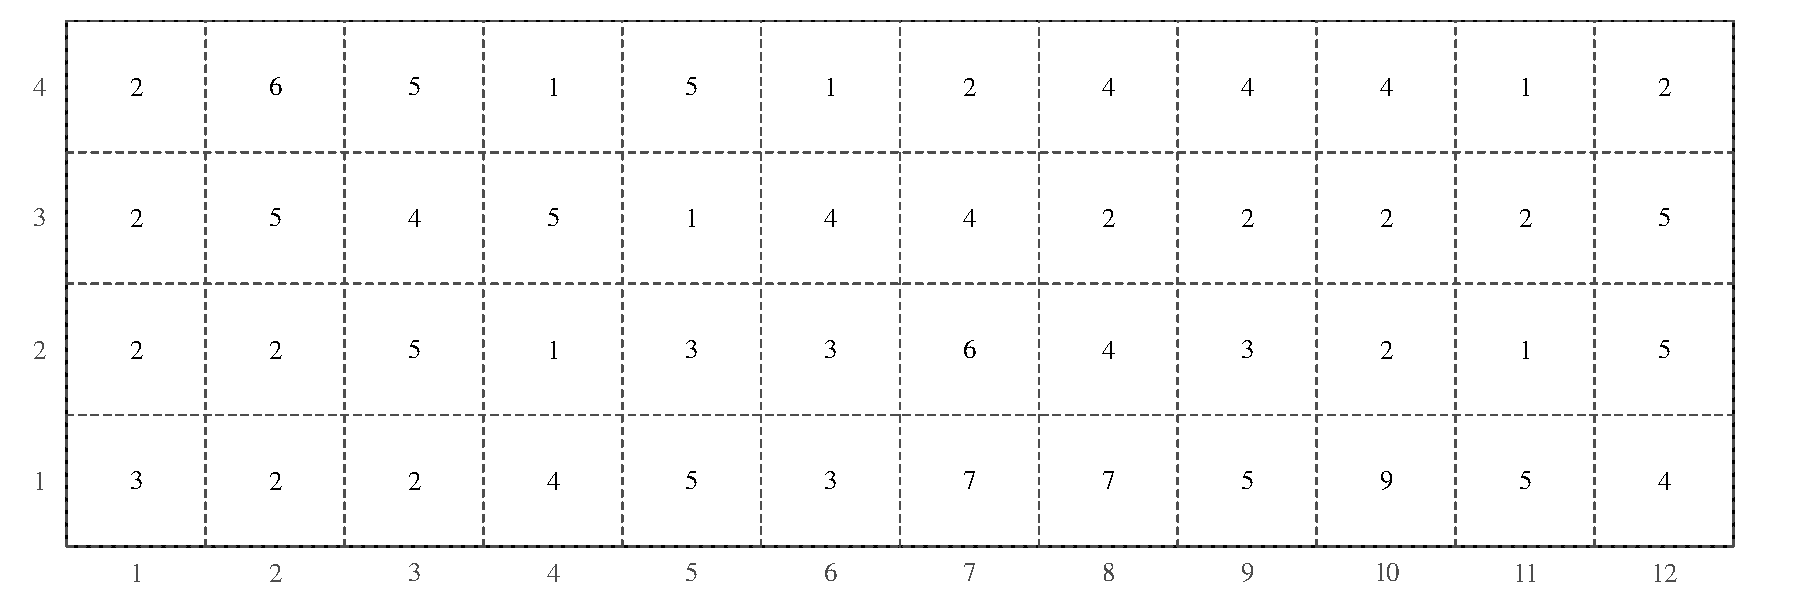
\includegraphics[width=\textwidth]{../figures/zirconcounts.pdf}
\begingroup \captionof{figure}{The number of zircons counted in each
  square of Figure~\ref{fig:zircons}.\medskip}
\label{fig:zirconcounts}\endgroup

\noindent and tallying the number of zircons per square in a histogram:

\noindent\begin{minipage}[t][][b]{.3\textwidth}
  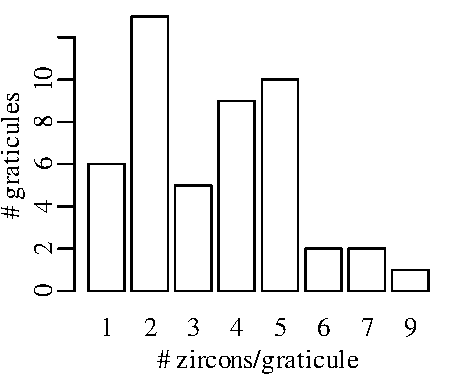
\includegraphics[width=\textwidth]{../figures/zirconhist.pdf}\medskip
\end{minipage}
\begin{minipage}[t][][t]{.7\textwidth}
  \captionof{figure}{ Histogram of the zircon counts shown in
    Figure~\ref{fig:zirconcounts}.\medskip
    ~\\
    \textbf{mean: 3.50}\\
    standard deviation: 1.85\\
    \textbf{variance: 3.40}
  }
  \label{fig:zirconhist}
\end{minipage}

Like the earthquake example, also this zircon example is characterised
by similar values for the mean and the variance. This turns out to be
a characteristic property of the Poisson distribution.

\section{Probability mass function}
\label{sec:PMF}

The Poisson distribution expresses the probability of a given number
of events occurring in a fixed interval of time or space if these
events occur with a \textbf{constant mean rate} and are
\textbf{independent} of the time since the last event. Examples of
Poisson variables include the number of

\begin{enumerate}
\item people killed by lightning per year;
\item mutations in DNA per generation;
\item radioactive disintegrations per unit time;
\item mass extinctions per 100 million years.
\end{enumerate}

The number of earthquakes including aftershocks and the number of
floods per year are \emph{not} Poisson variables, because they are
clustered in time. The Poisson distribution predicts the probability
of observing the number of `successes' $k$ given the long term average
of successes $\lambda$:
\begin{equation}
  P(k|\lambda) = \frac{\lambda^k e^{-\lambda}}{k!}
  \label{eq:poispmf}
\end{equation}

Thus the Poisson distribution is characterised by a single parameter,
$\lambda$. Exploring the distribution for different values of this
parameter:\medskip

\noindent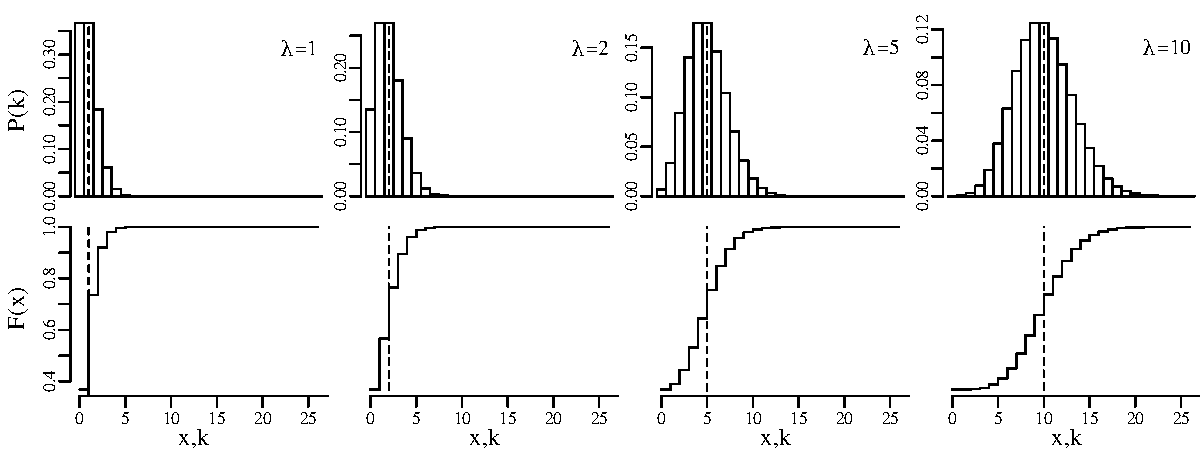
\includegraphics[width=\textwidth]{../figures/increasinglambda.pdf}
\begingroup \captionof{figure}{PMF (top) and CDF (bottom) of the
  Poisson distribution for different values of the parameter
  $\lambda$, as marked by the dashed lines.\medskip} \endgroup

The Poisson distribution is positively skewed but becomes more
symmetric with increasing $\lambda$. In this respect it is similar to
the binomial distribution (Figure~\ref{fig:binompower1}). In fact the
Poisson and binomial distributions are closely related to each
other. Recall that the binomial distribution depends on two
parameters: $n$ and $p$. It can be shown that the binomial
distribution converges to the Poisson distribution with increasing $n$
and decreasing $p$. In the limit of $n \rightarrow \infty$ and $p
\rightarrow 0$, the binomial distribution simplifies to a Poisson
distribution with $\lambda = {n}{p}$. The next table illustrates this
empirically by evaluating the probability of observing $k=2$
successes under a binomial distribution with $np=5$ for different
values of $n$ and $p$:

\begin{center}
\begin{tabular}{r|llllllll}
$n$ & 10  & 20   & 50  & 100  & 200   & 500  & 1,000 & 10,000\\
$p$ & 0.5 & 0.25 & 0.1 & 0.05 & 0.025 & 0.01 & 0.005 & 0.0005\\
$P(k=2)$ & 0.0439 & 0.0669 & 0.0779 & 0.0812 & 0.0827 & 0.0836 & 0.0839 & 0.0842
\end{tabular}
\captionof{table}{Binomial probability of 2 successes after $n$ trials
  for different values of $p$, where $np=5$. In the limit of $n
  \rightarrow{\infty}$ and $p \rightarrow{0}$, the cumulative
  probability $P(k=2)$ converges to a value of 0.0842. This equals the
  probability of 2 successes under a Poisson distribution with
  $\lambda = 5$.}
\end{center}

\section{Parameter estimation}
\label{sec:poispar}

The Poisson distribution has one unknown parameter, $\lambda$. This
parameter can be estimated using the method of maximum likelihood,
just like the parameter $p$ of the binomial distribution
(Section~\ref{sec:binompar}). As before, the likelihood function is
obtained by swapping the parameter ($\lambda$) and the data ($k$) in
the PMF function (Equation~\ref{eq:poispmf}):
\begin{equation}
  \mathcal{L}(\lambda|k) = \frac{\lambda^k e^{-\lambda}}{k!}
  \label{eq:poislik}
\end{equation}

And as before, we can estimate $\lambda$ by maximising the likelihood
function.  Thus, we take the derivative of $\mathcal{L}$ with respect
to $\lambda$ and set it to zero:
\begin{equation}
  \frac{\partial{\mathcal{L}}}{\partial{\lambda}} = 0
\end{equation}

Alternatively, we can also maximise the \textbf{log-likelihood}:
\begin{equation}
  \mathcal{LL}(\lambda|k) = k \ln[\lambda] - \lambda - \sum\limits_{i=1}^{k}i
  \label{eq:poisLL}
\end{equation}

\noindent and set its derivative w.r.t. $\lambda$ to zero:
\begin{equation}
  \frac{\partial{\mathcal{LL}}}{\partial{\lambda}} = 0
\end{equation}

Both approaches give exactly the same result because any parameter
value $\hat{\lambda}$ that maximises $\mathcal{L}$ also maximises
$\mathcal{LL}$.  Thus:
\begin{equation}
  \left.\frac{\partial{\mathcal{LL}}}{\partial{\lambda}}\right|_{\hat{\lambda}} =
  \frac{k}{\hat{\lambda}} - 1 = 0
\end{equation}

\noindent which leads to
\begin{equation}
  \frac{k}{\hat{\lambda}} = 1
\end{equation}

\noindent and, hence
\begin{equation}
  \hat{\lambda} = k
  \label{eq:lambda=k}
\end{equation}

In other words, the measurement itself equals the `most likely'
estimate for the parameter. However, this does not mean that all other
values of $\lambda$ are unlikely. In fact, other values of $\lambda$
may also be compatible with $k$, and \emph{vice versa}. The next
section explores which values of $\lambda$ are reconcilable with a
given value of $k$.

\section{Hypothesis tests}
\label{sec:poishyp}

Hypothesis testing for Poisson variables proceeds in exactly the same
way as for binomial variables (Section~\ref{sec:binomH}). For example:

\begin{enumerate}
\item Consider the following one-sided pair of hypotheses:

  \noindent\begin{minipage}{.4\textwidth}
    $H_0$ (\textbf{null hypothesis})
    
    \vspace{1em}
    
    $H_{\!A}$ (\textbf{alternative hypothesis}):
  \end{minipage}
  \begin{minipage}{.2\textwidth}
  \end{minipage}
  \begin{minipage}{.2\textwidth}
    $\lambda = 3.5$
    
    \vspace{1em}
    
    $\lambda>{3.5}$
  \end{minipage}
  \begin{minipage}{.2\textwidth}
  \end{minipage}\medskip

\item Like for the binomial case, the test statistic is the number of
  `successes'.  Suppose that we have observed $k=9$ successes.

\item The null distribution of the test statistic is a Poisson
  distribution with $\lambda={3.5}$:
  
  \begin{tabular}{c@{~}c@{~}c@{~}c@{~}c@{~}c@{~}c@{~}c@{~}c@{~}c@{~}c@{~}c}
    k & 0 & 1 & 2 & 3 & 4 & 5 & 6 & 7 & 8 & \textit{9} & 10 \\ \hline
    $P(T=k)$ & 0.030 & 0.106 & 0.185 & 0.216 & 0.189 &
    0.132 & 0.077 & 0.038 & 0.017 & \textit{0.007} & 0.002 \\
    $P({T}\geq{k})$ & 1.000 & 0.970 & 0.864 & 0.679 & 0.463 &
    0.275 & 0.142 & 0.065 & 0.027 & \textit{0.010} & 0.003 \\
  \end{tabular}

\item We will use the same significance level as always,
  i.e. $\alpha=0.05$.

\item Marking the rejection region in bold:

  \begin{tabular}{c@{~}c@{~}c@{~}c@{~}c@{~}c@{~}c@{~}c@{~}c@{~}c@{~}c@{~}c}
    k & 0 & 1 & 2 & 3 & 4 & 5 & 6 & 7 & \textbf{8} &
    \textbf{\textit{9}} & \textbf{10} \\ \hline
    $P(T=k)$ & 0.030 & 0.106 & 0.185 & 0.216 & 0.189 &
    0.132 & 0.077 & 0.038 & 0.017 & \textit{0.007} & 0.002 \\
    $P({T}\geq{k})$ & 1.000 & 0.970 & 0.864 & 0.679 & 0.463 &
    0.275 & 0.142 & 0.065 & \textbf{0.027} & \textbf{\textit{0.010}} &
    \textbf{0.003} \\
  \end{tabular}

\item\label{it:poisl351sided} The rejection region is $R =
  \{8,9,10,\ldots,\infty\}$, which includes our observation
  $k=9$. Therefore, our null hypothesis is rejected.

\end{enumerate}

Displaying the rejection region graphically:

\noindent\begin{minipage}[t][][b]{.6\textwidth}
  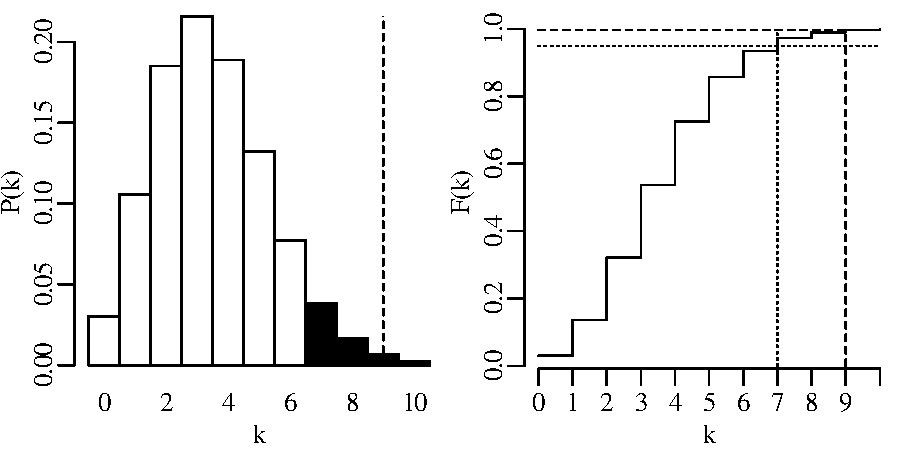
\includegraphics[width=\textwidth]{../figures/poishyp.pdf}\medskip
\end{minipage}
\begin{minipage}[t][][t]{.4\textwidth}
  \captionof{figure}{a) PMF and b) CDF of a Poissonian null
    distribution with $\lambda=3.5$. The rejection region is marked in
    black on a).  The horizontal dotted line in b) shows the
    $1-\alpha=0.95$ mark. The horizontal dashed line in the CDF marks
    the cumulative probability for $k=9$, which is greater than the
    0.95 cutoff. Therefore the one-sided null hypothesis is rejected.}
  \label{fig:poishyp}
\end{minipage}

\section{Multiple testing}
\label{sec:multipletesting}

The observant reader may have noticed that the hypothesis test of
Section~\ref{sec:poishyp} referred to the zircon counting example of
Figures~\ref{fig:zircons} -- \ref{fig:zirconcounts}. The average
number of observations per bin in this example was 3.5. Therefore,
according to Section~\ref{sec:poispar}, the maximum likelihood
estimate for $\lambda$ is 3.5 as well. According to our hypothesis
test, a value of $k=9$ is incompatible with a parameter value of
$\lambda=3.5$. Yet the observant reader may also have noticed that a
value of $k=9$ appears in the dataset
(Figure~\ref{fig:zirconcounts})!\medskip

Does this mean that our data do not follow a Poisson distribution?\medskip

The answer is no. The apparent contradiction between the
point-counting data and the hypothesis test is a result of multiple
hypothesis testing. To understand this problem, we need to go back to
the multiplicative rule of page~\pageref{page:multiplication}.  The
probability of incurring a type-I error is $\alpha$. Therefore, the
probability of not making a type-I error $1-\alpha=0.95$.  But this is
only true for one test. If we perform two tests, then the probability
of twice avoiding a type-I error is $(1-\alpha)^2=0.9025$. If we do
$N$ tests, then the probability of not making a type-I error reduces
to $(1-\alpha)^N$. Hence, the probability of making a type-I error
increases to $1-(1-\alpha)^N$. Figure~\ref{fig:zirconcounts} contains
${4}\times{12}=48$ squares. Therefore, the likelihood of a type-I
error is not $\alpha$ but $1-(1-\alpha)^{48}=0.915$.\medskip

In other words, there is a 91.5\% chance of committing a type-I error
when performing 48 simultaneous tests. One way to address this issue
is to reduce the confidence level of the hypothesis test from $\alpha$
to $\alpha/N$, where $N$ equals the number of tests.  This is called a
\textbf{Bonferroni correction}. In the case of our zircon example, the
confidence level would be reduced from $\alpha=0.05$ to
$\alpha=0.05/48=0.00104$ ($1-\alpha=0.99896$).  It turns out that the
99.896 percentile of a Poisson distribution with parameter
$\lambda=3.5$ is 10. So the observed outcome of $k=9$ zircons in the
48 square graticule is in fact not in contradiction with the null
hypothesis, but falls within the expected range of values.\medskip

Multiple testing is a common problem in science, and a frequent source
of spurious scientific `discoveries'. For example, consider a dataset
of 50 chemical elements measured in 100 samples. Suppose that you test
the degree of correlation between each of these elements and the gold
content of the samples. Then it is inevitable that one of the elements
will yield a `statistically significant' result. Without a
multi-comparison correction, this result will likely be spurious. In
that case, repetition of the same experiment on 100 new samples would
not show the same correlation. Poorly conducted experiments of this
kind are called statistical \emph{fishing expeditions}, \emph{data
  dredging} or \emph{p-hacking}. Sadly they are quite common in the
geological literature, and it is good to keep a sceptical eye out for
them.

\section{Confidence intervals}
\label{sec:poisCI}

The construction of confidence intervals for the Poisson parameter
$\lambda$ proceeds in pretty much the same way as it did for the
binomial parameter $p$. Let us construct a 95\% confidence interval
for $\lambda$ given the observation that $k=5$ magnitude 5.0 or
greater earthquakes occurred in the US in 2016.\medskip

The lower limit of a 95\% confidence interval for the number of
earthquakes per year is marked by the value of $\lambda$ that is more
than 2.5\% likely to produce an observation of $k=5$ or greater. This
turns out to be $\lambda=1.62$. The upper limit of the confidence
interval is marked by the value of $\lambda$ that is more than 97.5\%
likely to produce an observation of $k=5$ or smaller. This value is
$\lambda=11.7$. Hence, the 95\% confidence interval is $[1.62, 11.7]$.
Note that this interval includes the average of all the 100 preceding
years. \medskip

\noindent\begin{minipage}[t][][b]{.6\textwidth}
  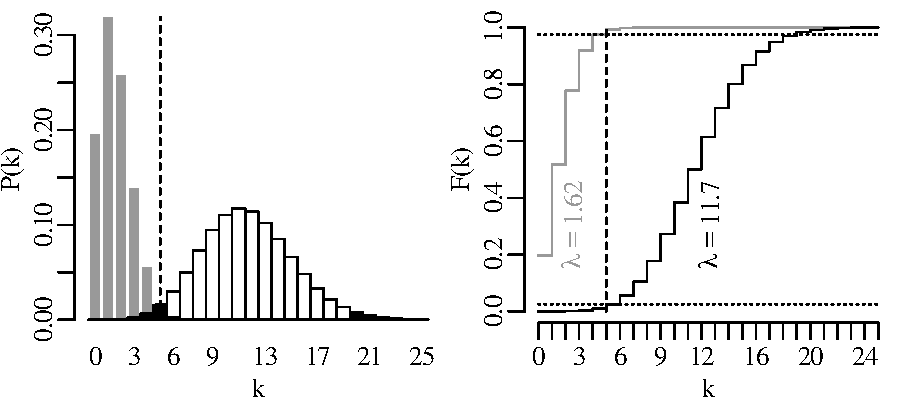
\includegraphics[width=\textwidth]{../figures/poisci.pdf}\medskip
\end{minipage}
\begin{minipage}[t][][t]{.4\textwidth}
  \captionof{figure}{95\% confidence interval for the Poisson
    parameter $\lambda$ given a single observation of $k=5$ events.
    The lower ($p=1.62$, grey) and upper ($p=11.67$) limits of the
    confidence interval are shown as a) PMFs and b) CDFs. Dotted
    horizontal lines mark the 0.025 and 0.975 confidence levels.}
  \label{fig:poisci}
\end{minipage}

Repeating the exercise for all observations in
Figure~\ref{fig:declusteredquakes} yields the following set of 100
confidence intervals for $\lambda$:\medskip

\noindent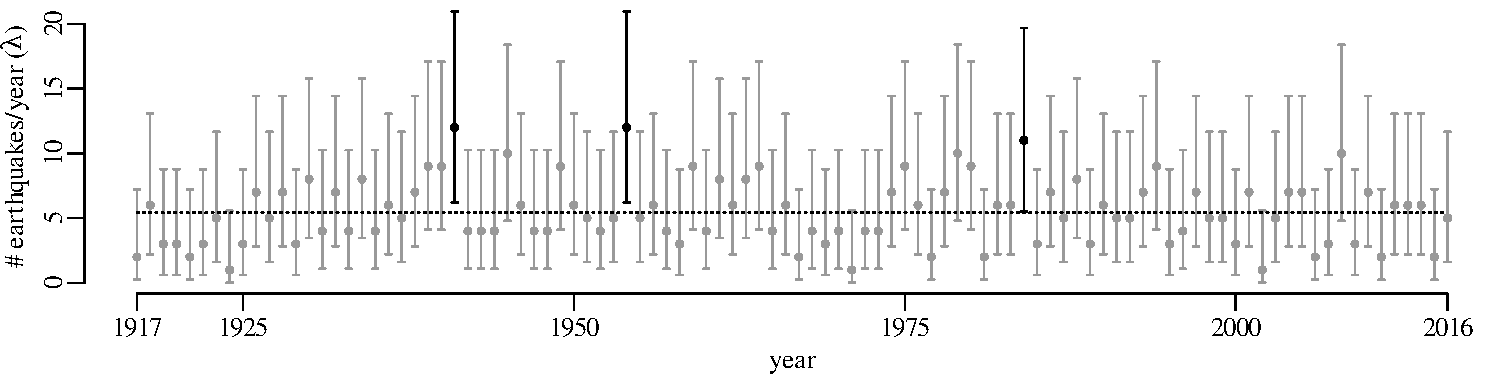
\includegraphics[width=\textwidth]{../figures/poiserrbars.pdf}
\begingroup \captionof{figure}{95\% Poisson confidence intervals for
  all the years in the declustered earthquake database. The horizontal
  dotted line marks the average of all the years
  ($\hat{\lambda}=5.43$). `outliers' are marked in black.\medskip}
\endgroup

Three years (1941, 1954 and 1984) stand out because their 95\%
confidence intervals do not overlap with the long term average value
of 5.43. Does this mean that the earthquake statistics did not fit the
Poisson distribution during those years? The answer to this question
is no, for the same reasons as given in
Section~\ref{sec:multipletesting}. When a large number of confidence
intervals are drawn, it is inevitable that some of these do not
include the true parameter value. In fact it would be suspicious if
all the error bars overlapped with the long term average.\medskip

With a confidence level of $\alpha=0.05$, there should be a 5\%
chance of committing a type-I error.  Therefore, we would expect 5\%
of the samples to be rejected, and 5\% of the error bars to exclude
the true parameter value. The observed number of rejected samples
(3/100) is in line with those expectations.


\chapter{The normal distribution}
\label{ch:normal}

The binomial (Chapter~\ref{ch:binomial}) and Poisson
(Chapter~\ref{ch:poisson}) distributions are just two of countless
possible distributions.  Here are a few examples of other
distributions that are relevant to Earth scientists:

\begin{itemize}

\item{\bf The negative binomial distribution} models the number of
  successes (or failures) in a sequence of Bernoulli trials before a
  specified number of failures (or successes) occurs. For example, it
  describes the number of dry holes $x$ that are drilled before $r$
  petroleum discoveries are made given a probability of discovery $p$:
  \begin{equation}
    P(x|r,p) = \binom{r+x-1}{x} (1-p)^x p^r
  \end{equation}

\item{\bf The multinomial distribution} is an extension of the
  binomial distribution where more than two outcomes are possible. For
  example, it describes the point counts of multiple minerals in a
  thin section. Let $p_1,p_2,\ldots,p_m$ be the relative proportions
  of $m$ minerals (where $\sum_{i=1}^{m}p_i=1$), and let
  $k_1,k_2,\ldots,k_m$ be their respective counts in the thin section
  (where $\sum_{i=1}^{m}k_i=n$). Then:
  \begin{equation}
    P(k_1,k_2,\ldots,k_m|p_1,p_2,\ldots,p_m) =
    \frac{n!}{\prod\limits_{i=1}^{m}k_i!} \prod\limits_{i=1}^{m}p_i^{k_i}
  \end{equation}

  The binomial and Poisson distributions are \textbf{univariate}
  distributions that aim to describe one-dimensional datasets. However
  the multinomial distribution is an example of a
  \textbf{multivariate} probability distribution, which describes
  multi-dimensional datasets.

\item{\bf The uniform distribution} is the simplest example of a
  \textbf{continuous distribution}. For any number $x$ between the
  minimum $a$ and maximum $b$:
  \begin{equation}
    f(x|a,b) =
  \begin{cases}
       \frac{1}{b-a} & \mbox{~if~} a \leq x \leq b\\
       0 & \mbox{~otherwise}
  \end{cases}
  \end{equation}
  
  $x$ does not have to be an integer but is free to take any decimal
  value. Therefore, $f(x|a,b)$ is not referred to as a probability
  mass function (PMF) but as a \textbf{probability density function}
  (PDF). Whereas PMFs are represented by the letter $P$, we use the
  letter $f$ to represent PDFs.  This is because the probability of
  observing any particular value $x$ is actually zero. For continuous
  variables, calculating probabilities requires integration between
  two values. For example:
  \begin{equation}
    P({c}\leq{x}\leq{d}) = \int\limits_{c}^{d} f(x|a,b) dx
  \end{equation}

  The cumulative density function (CDF) of a continuous variable is
  also obtained by integration rather than summation. For the uniform
  distribution:
  \begin{equation}
    P(X\leq{x}) =
    \begin{cases}
      0 & \mbox{~if~} x < a\\
      \int_{a}^{x} \frac{1}{b-a} dX = \frac{x-a}{b-a} & \mbox{~if~} a \leq x \leq b\\
      1 & \mbox{~if~} x > b
    \end{cases}
  \end{equation}

  Earthquakes follow a uniform distribution across the day, because
  they are equally likely to occur at 3:27:05 in the morning as they
  are at 17:02:58 in the afternoon, say.

\noindent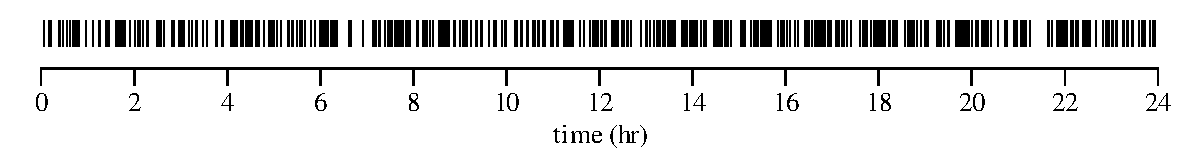
\includegraphics[width=\linewidth]{../figures/quakerug.pdf}
\begingroup \captionof{figure}{The time of day for all 543 magnitude
  5.0 or greater earthquakes of Figure~\ref{fig:declusteredquakes}.}
\endgroup
  
\end{itemize}

We will not discuss these, or most other distributions, in any detail.
Instead, we will focus our attention on one distribution, the Gaussian
distribution, which is so common that it is also known as the
\textbf{normal} distribution, implying that all other distributions
are `abnormal'.

\section{The Central Limit Theorem}
\label{sec:CLT}

Let us revisit the Old Faithful dataset of Figure~\ref{fig:KDE2D}.
  
\noindent\begin{minipage}[t][][b]{.35\textwidth}
  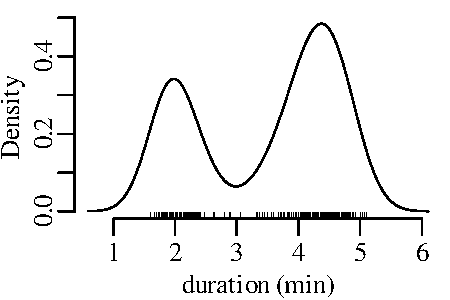
\includegraphics[width=\textwidth]{../figures/CLTfaithful1.pdf}\medskip
\end{minipage}
\begin{minipage}[t][][t]{.65\textwidth}
  \captionof{figure}{The KDE and rug plot of 272 Old Faithful eruption
    durations is the marginal distribution of
    Figure~\ref{fig:KDE2D}. This distribution has two modes at 2 and
    4.5 minutes.}
  \label{fig:CLTfaithful1}
\end{minipage}

The next three figures derive three new distributions by taking the
sum of $n$ randomly selected values from the geyser eruption
durations:

\noindent\begin{minipage}[t][][b]{.35\textwidth}
  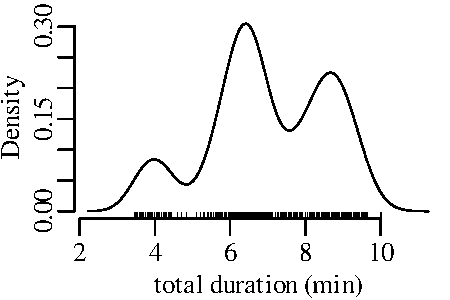
\includegraphics[width=\textwidth]{../figures/CLTfaithful2.pdf}\medskip
\end{minipage}
\begin{minipage}[t][][t]{.65\textwidth}
  \captionof{figure}{Collect $n=2$ randomly chosen events from the
    original dasaset of geyser eruptions with replacement and add
    their durations together. Repeat to create a new dataset of
    $N=500$ values.  The KDE of this distribution has not two but
    three modes at 4 ($=2\times{2}$), 6.5 ($=2+4.5$), and 9
    ($=2\times{4.5}$) minutes, respectively.}
  \label{fig:CLTfaithful2}
\end{minipage}

\noindent\begin{minipage}[t][][b]{.35\textwidth}
  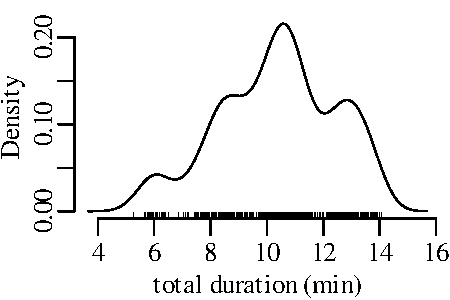
\includegraphics[width=\textwidth]{../figures/CLTfaithful3.pdf}\medskip
\end{minipage}
\begin{minipage}[t][][t]{.65\textwidth}
  \captionof{figure}{Collect $n=3$ randomly chosen events from the
    geyser eruption dataset and add their durations together. Repeat
    $N=500$ times to create a third dataset.  The KDE of this
    distribution has four visible modes, including peaks at 6
    ($=3\times{2}$), 8.5 ($=2\times{2}+4.5$), 11 ($=2+2\times{4.5}$)
    and 13.5 ($=3\times{4.5}$) minutes. }
  \label{fig:CLTfaithful3}
\end{minipage}

\noindent\begin{minipage}[t][][b]{.35\textwidth}
  \includegraphics[width=\textwidth]{../figures/CLTfaithful10.pdf}\medskip
\end{minipage}
\begin{minipage}[t][][t]{.65\textwidth}
  \captionof{figure}{Taking $N=500$ samples of $n=10$ randomly
    selected eruptions and summing their durations produces a fourth
    dataset whose KDE has a single mode with symmetric tails towards
    lower and higher values.}
  \label{fig:CLTfaithful10}
\end{minipage}

Figure~\ref{fig:CLTfaithful10} has the characteristic \emph{bell
  shape} of a Gaussian distribution, which is described by the
following PDF:
\begin{equation}
  f(x|\mu,\sigma) = \frac{1}{\sigma\sqrt{2\pi}}
  \exp\!\left[-\frac{(x-\mu)^2}{2\sigma^2}\right]
  \label{eq:gauss}
\end{equation}

\noindent where $\mu$ is the \textbf{mean} and $\sigma$ is the
\textbf{standard deviation}. It can be mathematically proven that the
\emph{sum} of $n$ randomly selected values converges to a Gaussian
distribution, provided that $n$ is large enough. This convergence is
guaranteed \textit{regardless of the distribution of the original
  data}.  This mathematical law is called the \textbf{Central Limit
  Theorem}.\medskip

The Gaussian distribution is known as the normal distribution because
it naturally arises from \emph{additive processes}, which are very
common in nature. It is easy to create normally distributed values in
a laboratory environment. There even exists a machine that generates
normally distributed numbers:

\noindent\begin{minipage}[t][][b]{.55\textwidth}
  \includegraphics[width=\textwidth]{../figures/galtonsbeanmachine.pdf}\medskip
\end{minipage}
\begin{minipage}[t][][t]{.45\textwidth}
  \captionof{figure}{Galton's bean machine is a mechanical device that
    simulates additive physical processes. It consists of a triangular
    arrangement of pegs above a linear array of containers.  When a
    bead enters the machine from the top, it bounces off the pegs on
    its way down to the containers. The probability of bouncing to the
    left is the same as the probability of bouncing to the
    right. After $n$ bounces, the bead lands in one of the containers,
    forming a bell shaped (binomial) distribution. With increasing
    $n$, this distribution converges to a Gaussian form.}
  \label{fig:galtonsbeanmachine}
\end{minipage}

Additive processes are very common in physics. For example, when a
drop of ink disperses in a volume of water, the ink molecules spread
by colliding with the water molecules.  This \emph{Brownian motion}
creates a Gaussian distribution, in which most ink molecules remain
near the original location ($\mu$), with wide tails in other
directions.

\section{The multivariate normal distribution}
\label{sec:multinorm}

The binomial, Poisson, negative binomial, multinomial, uniform and
univariate normal distributions are but a small selection from an
infinite space of probability distributions. These particular
distributions were given a specific name because they commonly occur
in nature.  However the majority of probability distributions do not
fall into a specific parametric category.  For example, the bivariate
distribution of Old Faithful eruption gaps and durations
(Figure~\ref{fig:KDE2D}) is not really captured by any of the
aforementioned distributions. In fact, it is quite easy to invent
one's own distributions. Here are four examples of such creations in
two-dimensional data space:\medskip

\noindent\includegraphics[width=\textwidth]{../figures/pop2d.pdf}
\begingroup \captionof{figure}{Four synthetic bivariate continuous
  distributions, defined by black areas and lines. White areas are
  excluded from the distributions.\medskip}
\label{fig:pop2d}
\endgroup

Let us collect $n=100$ random $(X,Y)$ samples from these four
distributions and plot them as four scatter plots:\medskip

\noindent\includegraphics[width=\textwidth]{../figures/rand2d.pdf}
\begingroup \captionof{figure}{It is easy to recognise the probability
  distributions of Figure~\ref{fig:pop2d} in the scatter plots of
  $n=100$ random points selected from them.\medskip}
\label{fig:rand2d}
\endgroup

Next, we can calculate the sum of all the sampled points in each of
the four panels in Figure~\ref{fig:rand2d}. This gives rise to four
new pairs of coordinates. Repeating this experiment $N=200$ times and
plotting the four resulting datasets as scatter plots:\medskip

\noindent\includegraphics[width=\textwidth]{../figures/rand2dsum.pdf}
\begingroup \captionof{figure}{Four scatter plots with $N=200$ points,
  each of which represents the sum of a random sample of $n=100$
  points drawn from Figure~\ref{fig:pop2d}.\medskip}
\label{fig:rand2sum}
\endgroup

Despite the completely different appearance of the four parent
distributions (Figure~\ref{fig:pop2d}) and samples
(Figure~\ref{fig:rand2d}), the distributions of their sums
(Figure~\ref{fig:rand2sum}) all look very similar. They consist of an
elliptical point cloud that is dense in the middle and thins out
towards the edges. The density of the points per unit area is
accurately described by a bivariate Gaussian distribution:
\begin{equation}
f(x,y|\mu_x,\mu_y,\sigma_x,\sigma_y,\sigma_{x,y}) = \frac{
\exp\left(-
\left[\begin{array}{@{}cc@{}}
(x-\mu_x) & (y-\mu_y)
\end{array}\right]
\left[\begin{array}{@{}c@{}c@{}}
\sigma^2_x & \sigma_{x,y}\\
\sigma_{x,y} & \sigma^2_y
\end{array}\right]^{-1}
\left[\begin{array}{@{}c@{}}
x-\mu_x\\
y-\mu_y
\end{array}\right] \biggl/ 2
\right)
}{2\pi\sqrt{
\left|\begin{array}{@{}c@{}c@{}}
\sigma^2_x & \sigma_{x,y}\\
\sigma_{x,y} & \sigma^2_y
\end{array}\right|
}}
\label{eq:2dgauss}
\end{equation}

This matrix expression is completely described by five parameters: the
means $\mu_x$ and $\mu_y$, the standard deviations $\sigma_x$ and
$\sigma_y$, and the covariance $\sigma_{x,y}$. One-dimensional
projections of the data on the X- and Y-axis yield two univariate
Gaussian distributions.

\noindent\begin{minipage}[t][][b]{.45\textwidth}
  \includegraphics[width=\textwidth]{../figures/norm2dmarginal.pdf}\medskip
\end{minipage}
\begin{minipage}[t][][t]{.55\textwidth}
  \captionof{figure}{The main panel shows population 4 of
    Figure~\ref{fig:rand2sum} as grey circles, and the best fitting
    bivariate Gaussian distribution as contours. The side panels show
    the marginal distributions of the $X$- and $Y$-variable, which are
    both univariate Gaussian. The means and standard deviations of the
    marginal distributions equal the means and the standard deviations
    of the bivariate distribution. The bivariate distribution has a
    fifth parameter, the covariance $\sigma_{x,y}$, which controls the
    angle at which the elliptical contours are rotated relative to the
    axes of the diagram. The significance of these parameters is
    further explored in Section~\ref{sec:normalproperties}.}
  \label{fig:norm2dmarginal}
\end{minipage}

\section{Properties}
\label{sec:normalproperties}

The univariate normal distribution is completely controlled by two
parameters:

\begin{enumerate}
\item The \textbf{mean} $\mu$ controls the \textbf{location} of the
  distribution.  Because the normal distribution is unimodal and
  symmetric, the mean also equals the median and the mode.
\item The \textbf{standard deviation} $\sigma$ quantifies the
  \textbf{dispersion} of the distribution.
\end{enumerate}

\noindent\includegraphics[width=\textwidth]{../figures/musigma.pdf}
\begingroup \captionof{figure}{PDFs of the univariate normal
  distribution for different values of $\mu$ and $\sigma$. $\mu$
  controls the position and $\sigma$ the width of the distribution. By
  definition, the area under the PDF always remains the same
  (i.e. $\int_{-\infty}^{+\infty}f(x)~dx = 1$).\medskip}
\label{fig:musigma}
\endgroup

The interval from $\mu-\sigma$ to $\mu+\sigma$ covers 68.27\% of the
area under the PDF, and the interval from $\mu-2\sigma$ to
$\mu+2\sigma$ covers 95.45\%. Conversely 95\% of the area under the
normal PDF is contained within an interval of $\mu\pm{1.96}\sigma$.

\noindent\includegraphics[width=\textwidth]{../figures/2sigma.pdf}
\begingroup \captionof{figure}{PDF (a) and CDF (b) of the normal
  distribution.  The $\mu\pm\sigma$ and $\mu\pm{2}\sigma$ intervals
  cover $\sim$68\% and $\sim$95\% of the distribution, respectively. }
\label{fig:2sigma}
\endgroup

\begin{enumerate}
  \setcounter{enumi}{2}
\item The \textbf{covariance} $\sigma_{x,y}$ controls the degree of
  \textbf{correlation} between two variables ($x,y$) in a bivariate
  normal distribution.
\end{enumerate}

\noindent\includegraphics[width=\textwidth]{../figures/cov.pdf}
\begingroup \captionof{figure}{The standard deviations $\sigma_x$ and
  $\sigma_y$, and covariance $\sigma_{x,y}$ control the shape and
  dispersion of the bivariate normal distribution.\medskip}
\label{fig:cov}
\endgroup

The 1$\sigma$ contour around the mean of a bivariate normal
distribution only covers 39\% of the probability instead of $68\%$ for
the univariate normal distribution, and the 2$\sigma$ interval covers
86\% of the probability instead of the 95\% of the univariate
distribution.

\section{Parameter estimation}
\label{sec:normalparameters}

$\mu$ and $\sigma$ are \emph{unknown} but can be \emph{estimated} from
the data. Just like the binomial parameter $p$
(Section~\ref{sec:binompar}) and the Poisson parameter $\lambda$
(Section~\ref{sec:poispar}), this can be done using the method of
maximum likelihood.  Given $n$ data points $\{x_1, x_2, \ldots,
x_n\}$, and using the multiplication rule, we can formulate the normal
likelihood function as
\begin{equation}
  \mathcal{L}(\mu,\sigma|x_1,x_2,\ldots,x_n) =
  \prod\limits_{i=1}^{n}f(x_i|\mu,\sigma)
  \label{eq:Lnorm}
\end{equation}

$\mu$ and $\sigma$ can be estimated by maximising the likelihood or,
equivalently, the log-likelihood:
\begin{equation}
  \begin{split}
    \mathcal{LL}(\mu,\sigma|x_1,x_2,\ldots,x_n) & =
    \sum\limits_{i=1}^{n}\ln\left[f(x_i|\mu,\sigma)\right] \\ & =
    \sum\limits_{i=1}^{n} -\ln[\sigma] - \frac{1}{2}\ln[2\pi] -
    \frac{(x_i-\mu)^2}{2\sigma^2}
  \end{split}
  \label{eq:LLnorm}
\end{equation}

Taking the derivative of $\mathcal{LL}$ with respect to $\mu$ and
setting it to zero:
\begin{equation}
  \begin{split}
    \left.\frac{\partial{\mathcal{LL}}}{\partial{\mu}}\right|_{\hat{\mu}} & =
    - \sum\limits_{i=1}^{n} \frac{x_i-\hat{\mu}}{\sigma^2} = 0 \\
    & \Rightarrow n\hat{\mu} - \sum\limits_{i=1}^{n} x_i = 0 \\
    & \Rightarrow \hat{\mu} = \frac{1}{n}\sum\limits_{i=1}^{n}x_i
  \end{split}
\end{equation}

\noindent which is the same as Equation~\ref{eq:mean}. Using the same
strategy to estimate $\sigma$:
\begin{equation}
  \label{eq:stdevgivenmu}
  \begin{split}
    \left.\frac{\partial{\mathcal{LL}}}{\partial{\sigma}}\right|_{\hat{\sigma}}
    & = \sum\limits_{i=1}^{n} - \frac{1}{\hat{\sigma}} +
    \frac{(x_i-\mu)^2}{\hat{\sigma}^3} = 0\\
    & \Rightarrow  \sum\limits_{i=1}^{n} \frac{(x_i-\mu)^2}{\hat{\sigma}^3} =
    \frac{n}{\hat{\sigma}} \\
    & \Rightarrow \hat{\sigma} =
    \sqrt{\frac{1}{n}\sum\limits_{i=1}^{n}(x_i-\mu)^2}\\
  \end{split}
\end{equation}

\noindent which is \emph{almost} the same as the formula for the
standard deviation that we saw in Section~\ref{sec:dispersion}
(Equation~\ref{eq:stdev}):
\begin{equation}
  s[x] = \sqrt{\frac{1}{n-1}\sum\limits_{i=1}^{n}(x_i-\bar{x})^2}
  \label{eq:stdevrepeat}
\end{equation}

There are just two differences between
Equations~\ref{eq:stdev}/\ref{eq:stdevrepeat} and
Equation~\ref{eq:stdevgivenmu}:
\begin{enumerate}
\item Equation~\ref{eq:stdevgivenmu} uses the population mean $\mu$,
  whereas Equation~\ref{eq:stdev} uses the sample mean $\bar{x}$.
\item Equation~\ref{eq:stdevgivenmu} divides the sum of the squared
  differences between the measurements and the mean by $n$, whereas
  Equation~\ref{eq:stdev} divides it by ($n-1$).
\end{enumerate}

The two differences are related to each other. The subtraction of 1
from $n$ is called the \textbf{Bessel correction} and accounts for the
fact that by using an estimate of the mean ($\bar{x}$), rather than
the true value of the mean ($\mu$), we introduce an additional source
of uncertainty in the estimate of the standard deviation. This
additional uncertainty is accounted for by subtracting one
\textbf{degree of freedom} from the model fit.\medskip

Finally, for multivariate normal datasets, we can show that (proof
omitted):
\begin{equation}
  \hat{\sigma}_{x,y} = \sum\limits_{i=1}^{n}\frac{1}{n}(x_i-\mu_x)(y_i-\mu_y)
\end{equation}

\noindent or, if $\mu_x$ and $\mu_y$ are unknown and must be estimated
from the data as well:
\begin{equation}
  s[x,y] = \sum\limits_{i=1}^{n}\frac{1}{n-1}(x_i-\bar{x})(y_i-\bar{y})
  \label{eq:sxy}
\end{equation}



\chapter{Error propagation}
\label{ch:errorprop}

Suppose that the extinction of the dinosaurs has been dated at 65 Ma
in one field location, and a meteorite impact has been dated at 64 Ma
elsewhere.  These two numbers are effectively meaningless in the
absence of an estimate of precision. Taken at face value, the dates
imply that the meteorite impact took place 1 million years after the
mass extinction, which rules out a causal relationship between the two
events. However, if the statistical uncertainty of the age estimates
is significantly greater than 1 Myr, then such of a causal
relationship remains plausible. There are two aspects of analytical
uncertainty:

\begin{itemize}
  \item{\bf accuracy} is the closeness of a statistical estimate to
    its true (but unknown) value.
  \item{\bf precision} is the closeness of multiple measurements to
    each other.
\end{itemize}

\noindent\includegraphics[width=\textwidth]{../figures/accuracyvsprecision.pdf}
\begingroup \captionof{figure}{Darts board illustration of accuracy
  (closeness to the centre) and precision (closeness of the
  measurements). The best case scenario combines high precision with
  high accuracy. The worst case scenario combines high precision with
  low accuracy. This is the worst possible situation because the high
  precision gives false confidence in the data.\\}
\label{fig:darts}
\endgroup

Accuracy can be assessed by analysing \emph{reference materials} (or
`secondary standards') whose true parameter values are known through
independent means. This procedure involves little statistics and won't
be discussed further in this chpater. Quantifying precision is a more
involved process that is also known as \textbf{error
  propagation}. This procedure will be discussed in some detail in the
following sections.

\section{Linear approximation}
\label{sec:linearerrorprop}

Suppose that the geological age or any other physical quantity ($z$)
is calculated as a function ($g$) of some measurements ($x$):
\begin{equation}
z = g(x)
\label{eq:zgx}
\end{equation}

\noindent and suppose that replicate measurements of $x$ ($x_i$, for
$i=1...n$) \emph{follow a normal distribution} with mean $\bar{x}$ and
standard deviation $s[x]$. Then these values can be used to estimate
$s[z]$, the standard deviation of the calculated value $z$.  If the
function $g$ is (approximately) linear in the vicinity of $\bar{x}$,
then small deviations $(\bar{x}-x_i)$ of the measured parameter $x_i$
from the mean value $\bar{x}$ are proporational to small deviations
$(\bar{z}-z_i)$ of the estimated quantity $z$ from the mean value
$\bar{z}=g(\overline{x})$.\\

Recall the definition of the sample standard deviation and variance
(Equation~\ref{eq:stdevrepeat}):

\begin{equation}
s[z]^2 \equiv \frac{1}{n-1} \sum_{i=1}^{n} (z_i-\bar{z})^2
\label{eq:varz}
\end{equation}

Let $\partial{z}/\partial{x}$ be the slope of the function $g$ with
respect to the measurements $x$, then:
\begin{equation}
(z_i-\bar{z}) \approx \frac{\partial z}{\partial x} (x_i-\bar{x})
\label{eq:zi-z}
\end{equation}

\noindent\begin{minipage}[t][][b]{.45\textwidth}
  \includegraphics[width=\textwidth]{../figures/errorprop2d.pdf}\\
\end{minipage}
\begin{minipage}[t][][t]{.55\textwidth}
\captionof{figure}{Error propagation of two linear functions, $g_1$
  (black line) and $g_2$ (grey line). The input data $\{x_i\}$ are
  normally distributed around some average value $\bar{x}$. Error
  propagation estimates the dispersion of the inferred quantity $z_i$
  from the dispersion of the measurements $x_i$.  Deviations
  $(x_i-\bar{x})$ from the average $x$-value are reduced (for function
  $g_1$) or magnified (for function $g_2$) depending on the slope of
  the functions, resulting in deviations of the dependent variable
  that are smaller $(z_{i1}-\bar{z}_1)$ or greater
  $(z_{i2}-\bar{z}_i)$ than $(x_i-\bar{x})$.  }
  \label{fig:errorprop2d}
\end{minipage}

Plugging Equation \ref{eq:zi-z} into \ref{eq:varz}, we obtain:

\begin{equation}
  \begin{split}
    s[z]^2 & \approx \frac{1}{n-1} \sum_{i=1}^{n}
    \left[(x_i-\overline{x}) \frac{\partial z}{\partial x}\right]^2 \\
    & = \left[\frac{\partial z}{\partial x}\right]^2 \left[\frac{1}{n-1}
      \sum_{i=1}^{n} (x_i-\overline{x})^2 \right] 
      = \left[\frac{\partial z}{\partial x}\right]^2 s[x]^2\\
    \Rightarrow s[z] & = \left|\frac{\partial z}{\partial x}\right| s[x]
  \end{split}
  \label{eq:errorprop1d}
\end{equation}

$s[z]$ is the \textbf{standard error} of $z$, i.e.  the
\textit{estimated} standard deviation of the inferred quantity $z$.\\

Equation~\ref{eq:errorprop1d} is the general equation for the
propagation of uncertainty with one variable.  Next, let us move on to
multivariate problems. Suppose that the our estimated quantity ($z$)
is calculated as a function ($g$) of two measurements ($x$ and $y$):

\begin{equation}
z = g(x,y)
\label{eq:zfxy}
\end{equation}

and further suppose that $x$ and $y$ follow a bivariate normal
distribution (Equation~\ref{eq:2dgauss}), then $\mu_x$, $\mu_{y}$,
$\sigma_{x}$, $\sigma_{y}$ and $\sigma_{x,y}$ can all be estimated (as
$\bar{x}, \bar{y}, s[x], s[y]$ and $s[x,y]$) from the input data
($\{x_i, y_i\}$, for $i~=~1...n$). These values can then be used to
infer $s[z]$, the standard error of $z$, in exactly the same way as
for the one dimensional case.\\

Differentiating $g$ with respect to $x$ and $y$:

\begin{equation}
  z_i - \overline{z} \approx (x_i-\overline{x}) \frac{\partial z}{\partial x} +
  (y_i-\overline{y}) \frac{\partial z}{\partial y}
  \label{eq:dg}
\end{equation}

Plugging Equation~\ref{eq:dg} into Equation~\ref{eq:varz}:

\begin{equation}
  s[z]^2 \approx \frac{1}{n-1} \sum_{i=1}^{n} \left[
    (x_i-\overline{x}) \frac{\partial z}{\partial x} +
    (y_i-\overline{y}) \frac{\partial z}{\partial y} \right]^2
\end{equation}

After some rearranging (similar the derivation of
Equation~\ref{eq:errorprop1d}), this leads to:

\begin{equation}
  s[z]^2 \approx s[x]^2 \left(\frac{\partial z}{\partial x}\right)^2 +
  s[y]^2 \left(\frac{\partial z}{\partial y}\right)^2 +
  2~s[x,y] \frac{\partial z}{\partial x} \frac{\partial z}{\partial y}
  \label{eq:errorprop2d}
\end{equation}

This is the general equation for the propagation of uncertainty with
two variables, which can also be written in a matrix form:

\begin{equation}
s[z]^2 \approx
\left[
\begin{array}{cc}
\frac{\partial z}{\partial x} \frac{\partial z}{\partial y}
\end{array}
\right]
\left[
\begin{array}{cc}
s[x]^2 & s[x,y]\\
s[x,y] & s[y]^2
\end{array}
\right]
\left[
\begin{array}{c}
\frac{\partial z}{\partial x} \\
\frac{\partial z}{\partial y}
\end{array}
\right]
\label{eq:errorprop2dmatrix}
\end{equation}

where the innermost matrix is known as the \emph{variance-covariance}
matrix and the outermost matrix (and its transpose) as the
\emph{Jacobian matrix}. The advantage of the matrix formulation is
that it can easily be scaled up to three or more dimensions.

\noindent\begin{minipage}[t][][b]{.55\textwidth}
  \includegraphics[width=\textwidth]{../figures/errorprop3d.pdf}\\
\end{minipage}
\begin{minipage}[t][][t]{.45\textwidth}
  \captionof{figure}{Error propagation of a bivariate function $z =
    g(x,y)$. The uncertainty in $z$ is \emph{approximately}
    proportional to the slope of the surface $g$ w.r.t. the
    measurements $x$ and $y$. If the curvature of the 3D surface is
    minor relative to the uncertainties, then said surface can be
    \emph{locally} approximated by a plane. Using such a linear
    approximation, the size of the error ellipses ($s[x]$, $s[y]$)
    around the mean measurements (black dots) linearly scales with
    corresponding deviations in the inferred quantity ($s[z]$).}
  \label{fig:errorprop3d}
\end{minipage}

\section{Examples}
\label{sec:errorpropexamples}

Equation~\ref{eq:errorprop2d}/\ref{eq:errorprop2dmatrix} is the
generic error propagation formula. This section will apply this
formula to some common mathematical functions. It will use the
following notation:

\begin{itemize}
\item{$a, b, c, \ldots$} are constants, i.e. values that are known
  without uncertainty ($s[a]=s[b]=s[c]=0$);
\item{$x$ and $y$} are measurements whose uncertainties ($s[x]$ and
  $s[y]$) were estimated from replicates;
\item{$z = g(x,y)$} is the estimated quantity.
\end{itemize}

\noindent For example, $z = x/2 + y^3$ can be written as $z = a x +
y^b$, where $a=1/2$ and $b=3$.

\begin{enumerate}
  
\item{\bf addition:}
  \[
  z = a + b x + c y
  \]

  Taking the derivatives of $z$ with respect to $x$ and $y$:
  
  \[
  \frac{\partial z}{\partial x} = b \mbox{~and~} \frac{\partial z}{\partial y} = c
  \]

  Plugging these into Equation~\ref{eq:errorprop2d}:

  \begin{equation}
    s[z]^2 = b^2 s[x]^2 + c^2 s[y]^2 + 2bc~s[x,y]
    \label{eq:addition}
  \end{equation}

  If $x$ and $y$ are uncorrelated (i.e., $s[x,y]=0$), then the
  variance of the sum equals the sum of the variances.

\item{\bf subtraction:}
  \[
  z = a x - b y
  \]

  The partial derivatives of $z$ with respect to $x$ and $y$ are

  \[
  \frac{\partial z}{\partial x} = a \mbox{~and~}
  \frac{\partial z}{\partial y} = -b
  \]

  Plugging these into Equation~\ref{eq:errorprop2d}:
  
  \begin{equation}
    s[z]^2 = a^2 s[x]^2 + b^2 s[y]^2 - 2ab~s[x,y]
    \label{eq:subtraction}
  \end{equation}

  Note that, if $x$ and $y$ are uncorrelated, then
  Equations~\ref{eq:addition} and \ref{eq:subtraction} are identical.

\item{\bf multiplication:}
  \[
  z = a x y
  \]

  The partial derivatives are

  \[
  \frac{\partial z}{\partial x} = a y \mbox{~and~}
  \frac{\partial z}{\partial y} = a x
  \]

  Plugging these into Equation~\ref{eq:errorprop2d}:

  \[
  s[z]^2 = (a y)^2 s[x]^2 + (a x)^2 s[y]^2 + 2(a y)(a x)~s[x,y]
  \]

  Dividing both sides of this equation by $z^2 = (a x y)^2$:
  
  \[
  \left(\frac{s[z]}{z}\right)^2 =
  \left(\frac{a y}{a x y} s[x]\right)^2 +
  \left(\frac{a x}{a x y} s[y]\right)^2 +
  2\left(\frac{a y}{a x y}\right)\left(\frac{a x}{a x y}\right) s[x,y]
  \]

  which simplifies to:

  \begin{equation}
    \left(\frac{s[z]}{z}\right)^2 = \left(\frac{s[x]}{x}\right)^2 +
    \left(\frac{s[y]}{y}\right)^2 + 2 \frac{s[x,y]}{x y}
    \label{eq:multiplication}
  \end{equation}

  $(s[x]/x)$ and $(s[y]/y)$ represent the \textit{relative standard
    deviation}s of $x$ and $y$. These are also known as the
  \textbf{coefficient}s \textbf{of variation} (CoV).  If $x$ and $y$
  are uncorrelated, then the squared CoVs of a product equals the sum
  of the squared CoVs.

\item{\bf division:}

  \[
  z = a \frac{x}{y}
  \]

  The partial derivatives are

  \[
  \frac{\partial z}{\partial x} = \frac{a}{y} \mbox{~and~}
  \frac{\partial z}{\partial y} = -\frac{a x}{y^2}
  \]

  Plugging these into Equation~\ref{eq:errorprop2d}:

  \[
  s[z]^2 = \left(\frac{a}{y}\right)^2 s[x]^2 +
  \left(-\frac{a x}{y^2}\right)^2 s[y]^2 +
  2\left(\frac{a}{y}\right)\left(-\frac{a x}{y^2}\right) s[x,y]
  \]

  Dividing both sides of this equation by $z^2 =
  \left(a x / y\right)^2$:
  
  \[
  s[z]^2 = \left(\frac{a}{y}\frac{y}{ax}\right)^2 s[x]^2 +
  \left(-\frac{a x}{y^2}\frac{y}{ax}\right)^2 s[y]^2 +
  2\left(\frac{a}{y}\frac{y}{ax}\right)
  \left(-\frac{a x}{y^2}\frac{y}{ax}\right) s[x,y]
  \]

  which simplifies to:

  \begin{equation}
    \left(\frac{s[z]}{z}\right)^2 = \left(\frac{s[x]}{x}\right)^2 +
    \left(\frac{s[y]}{y}\right)^2 - 2 \frac{s[x,y]}{x y}
    \label{eq:division}
  \end{equation}

  If $x$ and $y$ are uncorrelated, then the uncertainty of the
  quotient (Equation~\ref{eq:division}) equals the uncertainty of the
  product (Equation~\ref{eq:multiplication}).

\item{\bf exponentiation:}

  \[
  z = a e^{bx}
  \]

  The partial derivative of $z$ w.r.t. $x$ is

  \[
  \frac{\partial z}{\partial x} = ab e^{bx}
  \]

  Plugging this into Equation~\ref{eq:errorprop2d}:

  \[
  s[z]^2 = \left(ab e^{bx}\right)^2 s[x]^2
  \]

  Dividing both sides by $z^2 = \left(a e^{bx}\right)^2$:

  \[
  \left(\frac{s[z]}{z}\right)^2 =
  \left(\frac{ab e^{bx}}{a e^{bx}}s[x]\right)^2 
  \]

  which simplifies to

  \begin{equation}
    \left(\frac{s[z]}{z}\right)^2 = b^2 s[x]^2
    \label{eq:exponentiation}
  \end{equation}

\item{\bf logarithms:}

  \[
  z = a \ln[bx]
  \]

  The partial derivative of $z$ w.r.t. $x$ is

  \[
  \frac{\partial z}{\partial x} = \frac{a}{x}
  \]

  Plugging this into Equation~\ref{eq:errorprop2d}:

  \begin{equation}
    s[z]^2 = a^2 \left(\frac{s[x]}{x}\right)^2
    \label{eq:logarithms}
  \end{equation}

\item{\bf power:}

  \[
  z = a x^b
  \]

  The partial derivative of $z$ w.r.t. $x$ is

  \[
  \frac{\partial z}{\partial x} = ab x^{b-1}
  \]

  Plugging this into Equation~\ref{eq:errorprop2d}:

  \[
  s[z]^2 = \left(ab~x^{b-1}\right)^2 s[x]^2
  \]

  Dividing both sides by $z = a x^b$:

  \[
  \left(\frac{s[z]}{z}\right)^2 = \left(\frac{ab x^{b-1}}{a x^{b}}s[x]\right)^2 
  \]

  which simplifies to
  
  \begin{equation}
    \left(\frac{s[z]}{z}\right)^2 = b^2\left(\frac{s[x]}{x}\right)^2
    \label{eq:power}
  \end{equation}

\item{\bf other:}

  Error propagation for more complicated functions can either be derived
  from Equation~\ref{eq:errorprop2d} directly, or can be done with
  Equations~\ref{eq:addition}--\ref{eq:power} using the \textbf{chain
    rule}. For example, consider the following equation:

  \begin{equation}
    d = d_\circ + v_\circ t + g t^2
    \label{eq:newtons2nd}
  \end{equation}

  \noindent which describes the distance $d$ travelled by an object as a
  function of time $t$, where $d_\circ$ is the position at $t=0$,
  $v_\circ$ is the velocity at $t=0$, and $g$ is the acceleration.
  Although Equation~\ref{eq:newtons2nd} does not directly fit into any
  of the formulations that we have derived thus far, it is easy to
  define two new functions that do. Let

  \begin{equation}
    x \equiv d_\circ + v_\circ t
    \label{eq:xvt}
  \end{equation}

  \noindent and

  \begin{equation}
    y \equiv g t^2
    \label{eq:ygt2}
  \end{equation}

  \noindent then Equation~\ref{eq:xvt} matches with the formula for
  addition (Equation~\ref{eq:addition}):

  \[
  z = a + bx + cy
  \]

  \noindent where $a \equiv d_\circ$, $b \equiv v_\circ$, $x \equiv t$,
  $c \equiv 0$ and $y$ is undefined. Then uncertainty propagation of
  Equation~\ref{eq:xvt} using Equation~\ref{eq:addition} gives:

  \begin{equation}
    s[x]^2 = \left(v_\circ s[t]\right)^2
    \label{eq:sx}
  \end{equation}

  Similarly, Equation~\ref{eq:ygt2} matches with the formula for
  powering (Equation~\ref{eq:power}):

  \[
  z = a x^b
  \]

  \noindent where $a \equiv g$, $b \equiv 2$ and $x \equiv t$. Applying
  Equation~\ref{eq:power} to Equation~\ref{eq:ygt2} yields:

  \begin{equation}
    s[y]^2 = g^2 \left(\frac{s[t]}{t}\right)^2
    \label{eq:sy}
  \end{equation}

  Combining Equations~\ref{eq:xvt} and \ref{eq:ygt2} turns
  Equation~\ref{eq:newtons2nd} into a simple sum:

  \[
  d = x + y
  \]

  \noindent whose uncertainty can be propagated with
  Equation~\ref{eq:addition}:

  \[
  s[d]^2 = s[x]^2 + s[y]^2
  \]

  Substituting Equation~\ref{eq:sx} for $s[x]^2$ and
  Equation~\ref{eq:sy} for $s[y]^2$:

  \[
  s[d]^2 = \left(v_\circ s[t]\right)^2 + g^2 \left(\frac{s[t]}{t}\right)^2
  \]

  \noindent which leads to the following expression for the
  uncertainty of $d$:

  \begin{equation}
    s[d] = \sqrt{\left(v_\circ s[t]\right)^2 + g^2 \left(\frac{s[t]}{t}\right)^2}
    \label{eq:sdnewton}
  \end{equation}

  To illustrate the use of this formula, suppose that $d_\circ=0$~m,
  $v_\circ=10$~m/s and $g=9.81$~m/s\textsuperscript{2}.  Further
  suppose that we measure the time $t$ with a watch that has a 1
  second precision ($s[t]=1$). Then we can predict how far the object
  will have travelled after 5 seconds:

  \begin{equation}
  d = 0 \mbox{~m} +
  10 \frac{\mbox{m}}{\mbox{s}} \times 5 \mbox{~s} +
  9.81\frac{\mbox{m}}{\mbox{s}^2} \times (5 \mbox{~s})^2 = 295.25\mbox{~m}
  \label{eq:snowy}
  \end{equation}

  Using Equation~\ref{eq:sdnewton}, the uncertainty of $d$ is given
  by:

  \begin{equation}
  s[d] = \sqrt{\left(10 \frac{\mbox{m}}{\mbox{s}} \times 1\mbox{~s}\right)^2 +
    \left(9.81\frac{\mbox{m}}{\mbox{s}^2}\right)^2
    \left(\frac{1\mbox{~s}}{5\mbox{~s}}\right)^2} = 10.19\mbox{~m}
  \label{eq:haddock}
  \end{equation}

  Thus the estimated displacement after 10~seconds can be reported as
  $295.25\pm{10.19}$~m, or as $295\pm{10}$~m if we \textbf{round} the
  estimate to two \textbf{significant digits}. Note how
  Equations~\ref{eq:snowy} and \ref{eq:haddock} specifies the units of
  all the variables. Checking that these units are balanced is good
  practice that avoids arithmetic errors.
  
\end{enumerate}

\section{Standard deviation vs. standard error}
\label{sec:stderr}

As defined in Section~\ref{sec:linearerrorprop}, the standard error is
the estimated standard deviation of some derived quantity obtained by
error propagation. The mean of set of numbers is an example of such a
derived quantity, and its estimated uncertainty is called the standard
error of the mean.  Let $\{x_1,x_2, \ldots x_n\}$ be $n$ measurements
of some quantity $x$, and let $\bar{x}$ be its mean
(Equation~\ref{eq:mean}):

\[
\bar{x} = \sum\limits_{i=1}^n \frac{x_i}{n} = \frac{1}{n} \sum\limits_{i=1}^n x_i
\]

Applying the error propagation formula for a sum
(Equation~\ref{eq:addition}):

\[
s[\bar{x}]^2 = \sum\limits_{i=1}^{n}\left(\frac{s[x_i]}{n}\right)^2 =
\left(\frac{1}{n}\right)^2 \sum\limits_{i=1}^{n}s[x_i]^2
\]

If all the $x_i$s were drawn from the same normal distribution with
standard deviation $s[x]$, then

\[
s[\bar{x}]^2 = \left(\frac{1}{n}\right)^2 \sum\limits_{i=1}^{n}s[x]^2 =
n \left(\frac{1}{n}\right)^2 s[x]^2
\]

\noindent which simplifies to

\begin{equation}
  s[\bar{x}] = \frac{s[x]}{\sqrt{n}}
  \label{eq:stderrmean}
\end{equation}

The standard error of the mean monotonically decreases with the square
root of sample size. In other words, we can arbitrarily increase the
\emph{precision} of our analytical data by acquiring more
data. However, it is important to note that the same is generally not
the case for the \emph{accuracy} of those data
(Figure~\ref{fig:darts}). To illustrate the effect of the square root
rule, consider the statistics of human height as an example.  The
distribution of the heights of adult people is approximately normal
with a mean of 165~cm and a standard deviation of 10~cm. There about 5
billion adult humans on the planet. Averaging their heights should
produce a value of 165~cm with a standard error of
$10/\sqrt{5\times{10}^9} = 1.4\times{10}^{-4}$~cm. So even though
there is a lot of dispersion among the heights of humans, the standard
error of the mean is only 1.5 \emph{microns}.

\section{Fisher Information}
\label{sec:FisherInformation}

We used the method of maximum likelihood to estimate the parameters of
the binomial (section~\ref{sec:binompar}), Poisson
(section~\ref{sec:poispar}) and normal
(section~\ref{sec:normalparameters}) distributions. An extension of
the same method can be used to estimate the standard errors of the
parameters without any other information. Let $\hat{z}$ be the maximum
likelihood estimate of some parameter $z$. We can approximate the
log-likelihood with a second order Taylor series in the vicinity of
$\hat{z}$:

\[
  \mathcal{LL}(z) \approx \mathcal{LL}(\hat{z}) +
  \frac{\partial\mathcal{LL}}{\partial{z}} (z-\hat{z}) +
  \frac{1}{2} \frac{\partial^2\mathcal{LL}}{\partial{z^2}} (z-\hat{z})^2
\]

By definition, $\partial{\mathcal{LL}}/\partial{z}=0$ at
$\hat{z}$. Therefore, the likelihood ($\mathcal{L}(z) =
\exp[\mathcal{LL}(z)]$) is proportional to:

\[
\mathcal{L}(z) \propto 
\exp\left[
  \frac{1}{2} \frac{\partial^2\mathcal{LL}}{\partial{z^2}} (z-\hat{z})^2
  \right]
\]

\noindent which can also be written as:

\[
\mathcal{L}(z) \propto \exp\!\left[
  -\frac{1}{2} \frac{(z-\hat{z})^2}{
    -\frac{1}{\frac{\partial^2\mathcal{LL}}{\partial{z^2}}}
  }\right]
\]

This equation fits the functional form of the normal distribution
(Equation~\ref{eq:gauss}):

\[
\mathcal{L}(z) \propto \exp\!\left[
  -\frac{1}{2} \frac{(z-\hat{z})^2}{\sigma[z]^2}
  \right]
\]

\noindent which leads to

\begin{equation}
  \sigma[z]^2 = \frac{1}{-\frac{\partial^2\mathcal{LL}}{\partial{z^2}}}
  \label{eq:Fisher}
\end{equation}

$-\frac{\partial^2\mathcal{LL}}{\partial{z^2}}$ is known as the
\textbf{Fisher Information}. Equation~\ref{eq:Fisher} can be
generalised to multiple dimensions:

\begin{equation}
  \Sigma = -\mathcal{H}^{-1}
  \label{eq:multidimFisher}
\end{equation}

\noindent where $\Sigma$ is the covariance matrix and
$(\mathcal{H})^{-1}$ is the inverse of the (`Hessian') matrix of
second derivatives of the log-likelihood function with respect to the
parameters.\\

To illustrate the usefulness of Equation~\ref{eq:Fisher}, let us apply
it to the Poisson distribution.  Recalling the log-likelihood function
(Equation~\ref{eq:poisLL}) and denoting the maximum likelihood
estimate of the parameter by $\hat{\lambda}$:

\[
\mathcal{LL}(\hat{\lambda}|k) =
k \log[\hat{\lambda}] - \hat{\lambda} - \sum\limits_{i=1}^{k}i
\]

Taking the second derivative of $\mathcal{LL}$ with respect to
$\hat{\lambda}$:

\begin{equation}
  \frac{\partial^2{\mathcal{LL}}}{\partial{\hat{\lambda}^2}} =
  -\frac{k}{\hat{\lambda}^2}
  \label{eq:d2LLdl2}
\end{equation}

Plugging Equation~\ref{eq:d2LLdl2} into \ref{eq:Fisher}:

\[
  \sigma[\hat{\lambda}]^2 = \frac{\hat{\lambda}^2}{k}
\]

Recalling that $\hat{\lambda} = k$ (Equation~\ref{eq:lambda=k}), we
get

\begin{equation}
  \sigma[\hat{\lambda}]^2 = \hat{\lambda}
  \label{eq:poisvar}
\end{equation}

Thus we have proven that the variance of a Poisson variable equals its
mean, which was already shown empirically in Chapter~\ref{ch:poisson}.


\chapter{Comparing distributions}
\label{ch:comparingdistributions}

The previous chapters have introduced a plethora of parametric
distributions that allow us to test hypotheses and assess the
precision of experimental results. However, these inferences are only
as strong as the assumptions on which they are based.  For example,
Chapter~\ref{ch:binomial} used a binomial distribution to assess the
occurrence of gold in a prospecting area, assuming that the gold was
randomly distributed across all the claims; and
Chapter~\ref{ch:poisson} used a Poisson distribution to model
earthquakes, assuming that the earthquake catalog was free of clusters
and that all aftershocks had been removed from it. This chapter will
introduce some strategies to test these assumptions, both graphically
and numerically.

\section{Q-Q plots}
\label{sec:q-q}

As the name suggests, a quantile-quantile or Q-Q plot is a graphical
method for comparing two probability distributions by plotting their
quantiles against each other. Q-Q plots set out the quantiles of a
sample against those of a theoretical distribution, or against the
quantiles of another sample. For example, comparing the Old Faithful
eruption duration dataset (Figure~\ref{fig:CLTfaithful1}) to a normal
distribution:

\noindent\begin{minipage}[t][][b]{.3\textwidth}
  \includegraphics[width=\textwidth]{../figures/qqfaithful1.pdf}\medskip
\end{minipage}
\begin{minipage}[t][][t]{.7\textwidth}
  \captionof{figure}{Quantile-quantile (Q-Q) plot of Old Faithful
    eruption durations. The horizontal axis marks the theoretical
    quantiles of a normal distribution with the same mean and standard
    deviation as the data. The vertical axis marks the quantiles of
    the actual data. If the two distributions being compared are
    similar, the points in the Q-Q plot will approximately lie on the
    line y = x. Otherwise they will not. In this example the
    distribution of eruption durations clearly does not follow a
    normal distribution.}
  \label{fig:qqfaithful1}
\end{minipage}

\noindent\begin{minipage}[t][][b]{.3\textwidth}
  \includegraphics[width=\textwidth]{../figures/qqfaithful2.pdf}\medskip
\end{minipage}
\begin{minipage}[t][][t]{.7\textwidth}
  \captionof{figure}{Q-Q plot of the dataset of 500 sums of $n = 2$
    randomly selected eruption durations shown in
    Figure~\ref{fig:CLTfaithful2}. The resulting trimodal distribution
    plots closer to the 1:1 line than the original dataset of
    Figure~\ref{fig:qqfaithful1} but is still far from normal.}
  \label{fig:qqfaithful2}
\end{minipage}

\noindent\begin{minipage}[t][][b]{.3\textwidth}
  \includegraphics[width=\textwidth]{../figures/qqfaithful10.pdf}\medskip
\end{minipage}
\begin{minipage}[t][][t]{.7\textwidth}
  \captionof{figure}{Q-Q plot of the dataset of 500 sums of $n = 10$
    randomly selected eruption durations shown in
    Figure~\ref{fig:CLTfaithful10}. The data plot very close to the
    1:1 line, visually confirming that they follow a normal
    distribution.  The sample distribution only deviates from the
    theoretical distribution at the most extreme quantiles. This
    indicates that the sample distribution has heavier tails than the
    normal distribution. This phenomenon will be discussed further in
    the next section. Increasing $n$ further would remove this effect
    near the tails and bring the sample distribution even closer to
    the normal distribution.}
  \label{fig:qqfaithful10}
\end{minipage}

Q-Q plots cannot only be used to compare sample distributions with
theoretically predicted parametric distributions, but also to compare
one sample with another. For example:

\noindent\begin{minipage}[t][][b]{.3\textwidth}
  \includegraphics[width=\textwidth]{../figures/qqfaithful12.pdf}\medskip
\end{minipage}
\begin{minipage}[t][][t]{.7\textwidth}
  \captionof{figure}{ Q-Q plot comparing datasets
    $x_1=\mbox{sum}(X_1)$ and $x_2=\mbox{sum}(X_2)$ of
    Figure~\ref{fig:rand2sum}. Even though the two datasets have
    markedly different means ($\bar{x}_1=50.0$ and $\bar{x}_2=59.9$)
    and slightly different standard deviations ($s[x_1]=3.3$ and
    $s[x_2]=3.1$), the quantiles of the two datasets plot along a
    straight line. This means that their distributions are identical
    in shape.  }
  \label{fig:qqfaithful12}
\end{minipage}

\section{The t-test}
\label{sec:t}

The Q-Q plot in Figure~\ref{fig:qqfaithful12} compared two samples
that were normally distributed with different means.  However, it may
not be clear if the difference between the means is statistically
significant or not. Before we address this problem, let us first look
at a related but slightly simpler problem. Consider the density of 5
gold coins as an example:

\begin{center}
\begin{tabular}{c|ccccc}
  coin \# & 1 & 2 & 3 & 4 & 5 \\ \hline
  density (g/cm\textsuperscript{3}) & 19.09 & 19.17 & 19.31 & 19.07 & 19.18
  \label{tab:coins}
\end{tabular}
\end{center}

The density of pure gold is 19.30~g/cm\textsuperscript{3}. We might
ask ourselves the question if the five coins are made of pure gold, or
if they consist of an alloy that mixes gold with a less dense metal?
To answer this question, we assume that the sample mean $\bar{x}$
follows a normal distribution with mean $\mu$ and standard deviation
$\sigma/\sqrt{n}$ (following the same derivation as
Equation~\ref{eq:stderrmean}). Thus, the parameter
\begin{equation}
  z = \frac{\bar{x}-\mu}{\sigma/\sqrt{n}}
  \label{eq:z}
\end{equation}

\noindent follows a \textbf{standard normal distribution} whose mean
is zero and whose standard deviation is one. As we have seen in
Section~\ref{sec:normalparameters}, $\sigma$ is unknown but can be
estimated by the sample standard deviation $s[x]$. We can then
replace Equation~\ref{eq:z} with a new parameter
\begin{equation}
  t = \frac{\bar{x}-\mu}{s[x]/\sqrt{n}}
  \label{eq:t}
\end{equation}

However, $t$ does not follow a normal distribution but a
\textbf{Student t-distribution} with $(n-1)$ \textbf{degrees of
  freedom} where the $(n-1)$ plays a similar role as the Bessel
correction of Section~\ref{sec:normalparameters}. It accounts for the
`double use' of the data to estimate both the mean and the standard
deviation of the data. The t-distribution forms the basis of a
statistical test that follows the same sequence of steps as used in
Sections~\ref{sec:binomH} and \ref{sec:poishyp}.

\begin{enumerate}
\item  Formulate two hypotheses:\medskip

  \noindent\begin{minipage}{.4\textwidth}
    $H_0$ (\textbf{null hypothesis})
    
    \vspace{1em}
    
    $H_{\!A}$ (\textbf{alternative hypothesis}):
  \end{minipage}
  \begin{minipage}{.2\textwidth}
  \end{minipage}
  \begin{minipage}{.2\textwidth}
    $\mu=19.30$
    
    \vspace{1em}
    
    $\mu<{19.30}$
  \end{minipage}
  \begin{minipage}{.2\textwidth}
  \end{minipage}
  
\item Calculate the following test statistic:

  \begin{equation}
    t = \frac{\bar{x} - \mu_\circ}{s[x]/\sqrt{n}}
    \label{eq:t1}
  \end{equation}

  \noindent where $\bar{x} = 19.164$, $\mu_\circ = 19.30$, 
  $s[x] = 0.0948$, and $n = 5$ so that $t = -3.2091$.

\item Under $H_0$, Equation~\ref{eq:t1} follows a Student
  t-distribution with 4 degrees of freedom. Tabulating some key
  quantiles of this distribution:

  \begin{center}
    \begin{tabular}{c|c@{\gap}c@{\gap}c@{\gap}c@{\gap}
        c@{\gap}c@{\gap}c@{\gap}c@{\gap}c@{\gap}c@{\gap}c@{\gap}c}
      $t$ & -3.75 & \textit{-3.2091} & -2.78 & -2.13 & -1.53 & -0.74 &
      0 & 0.74 & 1.53 & 2.13 & 2.78 & 3.75 \\ \hline
      $P(T\leq{t})$ & 0.01 & \textit{0.0163} & 0.025 & 0.05 & 0.1 & 0.25 &
      0.5 & 0.75 & 0.9 & 0.95 & 0.975 & 0.99
    \end{tabular}
  \end{center}

  \noindent where the observed value is marked in italics.
  
\item We will use the usual confidence level $\alpha = 0.05$.

\item Marking the rejection region ($P(T<t)<\alpha$) in bold:
  
  \begin{center}
    \begin{tabular}{c|c@{\gap}c@{\gap}c@{\gap}c@{\gap}
        c@{\gap}c@{\gap}c@{\gap}c@{\gap}c@{\gap}c@{\gap}c@{\gap}c}
      $t$ & \textbf{\textit{-3.75}} & \textbf{\emph{-3.2091}} & \textbf{-2.78} &
      \textbf{-2.13} & -1.53 & -0.74 & 0 & 0.74 & 1.53 & 2.13 & 2.78 & 3.75 \\ \hline
      $P(T\leq{t})$ & \textbf{0.01} & \textbf{\textit{0.0163}} & \textbf{0.025} &
      \textbf{0.05} & 0.1 & 0.25 & 0.5 & 0.75 & 0.9 &
      0.95 & 0.975 & 0.99
    \end{tabular}
  \end{center}

  The one-sided rejection region consists of all $t<-2.10$.

\item Because the observed value of $t=-3.2091$ falls inside the
  rejection region, the null hypothesis is rejected.

\end{enumerate}

We therefore conclude that the coins are not made of pure gold. Here
is a graphical representation of this test:

\noindent\begin{minipage}[t][][b]{.6\textwidth}
  \includegraphics[width=\textwidth]{../figures/1samplettest.pdf}\medskip
\end{minipage}
\begin{minipage}[t][][t]{.4\textwidth}
  \captionof{figure}{a) PDF and b) CDF of a t-distribution with 4
    degrees of freedom. The one-sided rejection region (for
    $\alpha=0.05$) is marked in black. The vertical dashed line marks
    the observed value of $t=-3.2091$. This line plots in the
    rejection region, leading to the conclusion that
    $\mu<{19.30}$~g/cm\textsuperscript{3}. The horizontal dashed line
    marks the p-value ($0.0163<\alpha$).}
  \label{fig:1samplettest}
\end{minipage}

The comparison between the mean of a sample (of coin densities) and a
particular value (19.30~g/cm\textsuperscript{3}) is called a
\textbf{one sample t-test}. If we want to compare the mean densities
of two samples, then this requires a \textbf{two sample t-test}. For
example, consider the following two collections of coins:

\begin{center}
\begin{tabular}{c|ccccc}
  coin \# & 1 & 2 & 3 & 4 & 5 \\ \hline
  density (1\textsuperscript{st} collection) &
  19.09 & 19.17 & 19.31 & 19.07 & 19.18 \\
  density (2\textsuperscript{nd} collection) &
  19.30 & 19.33 & 19.15 & 19.32
  \label{tab:2setcoins}
\end{tabular}
\end{center}

The average densities of collection~1 and 2 are 19.164~g/cm$^3$ and
19.275~g/cm$^3$, respectively. If we assume that the two collections
have the \textit{same variance}, then we can test whether the
difference between the two means is significant or not.

\begin{enumerate}
\item  Formulate two hypotheses:\medskip

  \noindent\begin{minipage}{.4\textwidth}
    $H_0$ (\textbf{null hypothesis})
    
    \vspace{1em}
    
    $H_{\!A}$ (\textbf{alternative hypothesis}):
  \end{minipage}
  \begin{minipage}{.2\textwidth}
  \end{minipage}
  \begin{minipage}{.2\textwidth}
    $\mu_1=\mu_2$
    
    \vspace{1em}
    
    $\mu_1\neq{\mu_2}$
  \end{minipage}
  \begin{minipage}{.2\textwidth}
  \end{minipage}
  
\item Calculate the following test statistic:
  \begin{equation}
    t = \frac{\bar{x}_1 - \bar{x}_2}{s_p\sqrt{\frac{1}{n_1}+\frac{1}{n_2}}}
    \label{eq:t2}
  \end{equation}

  \noindent where $\bar{x}_1 = 19.164$, $n_1 = 5$, $\bar{x}_2 =
  19.275$, $n_2 = 4$, and $s_p$ is the \emph{pooled} standard
  deviation:
  \begin{equation}
    s_p = \sqrt{\frac{(n_1-1) s[x_1]^2 + (n_2-1) s[x_2]^2}{n_1 + n_2 - 2}}
    \label{eq:sp}
  \end{equation}

  \noindent in which $s[x_1]=0.095$ and $s[x_2]=0.084$ are the
  standard deviations of the first and second coin collection,
  respectively. Plugging the data into equations \ref{eq:t2} and
  \ref{eq:sp} yields $t=-1.857$.

\item Under $H_0$, Equation~\ref{eq:t2} follows a Student
  t-distribution with $(n_1+n_2-2)$ degrees of freedom\footnote{Two
    degrees of freedom have been removed because we estimated two
    parameters from the data: $\bar{x}_1$ and
    $\bar{x}_2$.}. Tabulating some key quantiles of the t-distribution
  with 7 degrees of freedom:

  \begin{center}
    \begin{tabular}{c|c@{\gap}c@{\gap}c@{\gap}c@{\gap}
        c@{\gap}c@{\gap}c@{\gap}c@{\gap}c@{\gap}c@{\gap}c@{\gap}c}
      $t$ & -3.00 & -2.36 & -1.89 & \textit{-1.857} & -1.41 & -0.71 &
      0.00 & 0.71 & 1.41 & 1.89 & 2.36 & 3.00 \\ \hline
      $P(T\leq{t})$ & 0.01 & 0.025 & 0.05 & \textit{0.053} & 0.1 & 0.25 &
      0.5 & 0.75 & 0.9 & 0.95 & 0.975 & 0.99 \\
      $P(T\geq{t})$ & 0.99 & 0.975 & 0.95 & \textit{0.947} & 0.9 & 0.75 & 0.5 &
      0.25 & 0.1 & 0.05 & 0.025 & 0.01
    \end{tabular}
  \end{center}
  
  \noindent where the observed value is marked in italics.
  
\item We will use the conventional confidence level $\alpha =
  0.05$. But because we are carrying out a two-sided test, we will
  have two cutoff regions marked by $\alpha/2$ and $(1-\alpha/2)$,
  respectively.

\item Marking the rejection regions in bold:
  
  \begin{center}
    \begin{tabular}{c|c@{\gap}c@{\gap}c@{\gap}c@{\gap}
        c@{\gap}c@{\gap}c@{\gap}c@{\gap}c@{\gap}c@{\gap}c@{\gap}c}
      $t$ & \textbf{-3.00} & \textbf{-2.36} & 
      -1.89 & \emph{-1.857} & -1.41 & -0.71 & 0.00 & 0.71 & 1.41 & 1.89 &
      \textbf{2.36} & \textbf{3.00} \\ \hline
      $P(T\leq{t})$ & \textbf{0.01} & \textbf{0.025} &
      0.05 & \textit{0.053} & 0.1 & 0.25 &
      0.5 & 0.75 & 0.9 & 0.95 & 0.975 & 0.99 \\
      $P(T\geq{t})$ & 0.99 & 0.975 & 0.95 & \textit{0.947} & 0.9 & 0.75 & 0.5 &
      0.25 & 0.1 & 0.05 & \textbf{0.025} & \textbf{0.01}
    \end{tabular}
  \end{center}

  The two-sided rejection region consists of all $t<-2.40$ and all
  $t>{2.40}$.

\item Because the observed value of $t=-1.857$ falls outside the
  rejection region, we cannot reject the null hypothesis.

\end{enumerate}

\noindent\begin{minipage}[t][][b]{.6\textwidth}
  \includegraphics[width=\textwidth]{../figures/2samplettest.pdf}\medskip
\end{minipage}
\begin{minipage}[t][][t]{.4\textwidth}
  \captionof{figure}{a) PDF and b) CDF of a t-distribution with 7
    degrees of freedom. The two-sided rejection region (for
    $\alpha=0.05$) is marked in black. The vertical dashed line marks
    the observed value of $t=-1.857$ and plots outside the rejection
    region. Therefore the test does not allow us to conclude that
    $\mu_1\neq\mu_2$. }
  \label{fig:2samplettest}
\end{minipage}

\section{Confidence intervals}
\label{eq:tconf}

Section~\ref{sec:t} introduced a powerful way to test whether the mean
of a sample was equal to a particular value, or to the mean of another
sample. However, Section~\ref{sec:pitfalls} showed that formalised
tests such as the t-test have limited practical value. Provided that
the sample is large enough, its mean will nearly always be
`significantly' different than that of another sample. Suppose that we
were to average the densities of not five but five millions coins,
then it would be extremely unlikely for the mean to be exactly 19.30
g/cm\textsuperscript{3}. With a sample size of five million, the power
of the t-test would be such that even trace amounts of a lighter
contaminant would have a detectable effect on the density.\medskip

Instead of asking ourselves whether the coins have exactly the same
density as pure gold, it is more useful to know what the mean density
actually is, and to construct a confidence interval for it. We could
then use this information to learn something about the composition of
the coins. To construct a confidence interval for the mean, we follow
a similar procedure as laid out in Sections~\ref{sec:binomCI} and
\ref{sec:poisCI}. Let us use the first set of coins as an example, and
recall that the one sample t-statistic is defined as
(Equation~\ref{eq:t1}):
\[
  t = \frac{\bar{x} - \mu}{s[x]/\sqrt{n}}
\]

By definition, the 95\% confidence interval is the collection of all
those values of $\mu$ for which
\[
t_{df,\alpha/2} \leq t \leq t_{df,1-\alpha/2}
\]

\noindent where $t_{df,\alpha/2}$ and $t_{df,1-\alpha/2}$ are the
$\alpha/2$ and $(1-\alpha/2)$ quantiles of a t-distribution with $df$
degrees of freedom, respectively.  Hence:
\[
t_{df,\alpha/2} \leq \frac{\bar{x} - \mu}{s[x]/\sqrt{n}} \leq t_{df,1-\alpha/2}
\]

Rearranging:
\[
\bar{x} - t_{df,\alpha/2}\frac{s[x]}{\sqrt{n}} \geq \mu \geq
\bar{x} - t_{df,1-\alpha/2}\frac{s[x]}{\sqrt{n}}
\]

Because the t-distribution is symmetric around zero, we can also write:
\[
t_{df,1-\alpha/2} = -t_{df,\alpha/2}
\]

Hence
\[
\bar{x} + t_{df,\alpha/2}\frac{s[x]}{\sqrt{n}} \leq \mu \leq
\bar{x} - t_{df,\alpha/2}\frac{s[x]}{\sqrt{n}}
\]

\noindent or
\begin{equation}
  \mu \in \left\{\bar{x} \pm t_{df,\alpha/2}\frac{s[x]}{\sqrt{n}}\right\}
  \label{eq:tci}
\end{equation}

For the gold coin example of Section~\ref{sec:t}, $\bar{x}=19.164$,
$s[x]=0.0948$, $df=4$ and $t_{4,0.025}=-2.776$. Hence, the 95\%
confidence interval for $\mu$ is
$19.16\pm{0.12}$~g/cm\textsuperscript{3}. Note that this interval does
\emph{not} overlap with the density of pure gold
(19.30~g/cm\textsuperscript{3}), confirming again that the coins are
not made of pure gold. However, the upper limit of the 95\% confidence
interval is 19.28~g/cm\textsuperscript{3}, which is not far off the
19.30~g/cm\textsuperscript{3} value. Therefore, it is possible that
the amount of light contaminant is minor.\medskip

With increasing sample size, the t-distribution converges towards the
normal distribution:

\noindent\begin{minipage}[t][][b]{.6\textwidth}
  \includegraphics[width=\textwidth]{../figures/tdof.pdf}\medskip
\end{minipage}
\begin{minipage}[t][][t]{.4\textwidth}
  \captionof{figure}{a) PDFs and b) CDFs of the t-distribution for
    three different degrees of freedom ($df$). For small sample sizes
    (low $df$), the t-distribution has long tails towards low and high
    values. With increasing sample size, the tails become shorter and
    the t-distribution sharper. When $df>30$, the t-distribution is
    almost indistinguishable from a standard normal distribution with
    $\mu=0$ and $\sigma=1$.}
  \label{fig:tdof}
\end{minipage}

Evaluating $t_{df,0.975}$ for different values of $df$:

\begin{center}
  \begin{tabular}{c|c@{\gap}c@{\gap}c@{\gap}c@{\gap}c@{\gap}c
      @{\gap}c@{\gap}c@{\gap}c@{\gap}c@{\gap}c@{\gap}c@{\gap}c}
    $df$ & 1 & 2 & 3 & 4 & 5 & 6 & 7 & 8 & 9 & 10 & 30 & 100 & 1000 \\
    $t_{df,0.975}$ &  12.710 & 4.303 & 3.182 & 2.776 & 2.571 &
    2.447 & 2.365 & 2.306 & 2.262 & 2.228 & 2.042 & 1.984 & \textbf{1.962}
  \end{tabular}
\end{center}

For large sample sizes, the 95\% percentile of the t-distribution is
the same as the 95\% percentile of the normal distribution ($=1.962$,
see Section~\ref{sec:normalproperties}). In this case
Equation~\ref{eq:tci} simplifies to approximately
\[
\mu \in \left\{ \bar{x} \pm 2 s[\bar{x}] \right\}
\]

\noindent where $s[\bar{x}]$ is the standard error of the mean
(Equation~\ref{eq:stderrmean}).

\noindent\begin{minipage}[t][][b]{.6\textwidth}
  \includegraphics[width=\textwidth]{../figures/normconf.pdf}\medskip
\end{minipage}
\begin{minipage}[t][][t]{.4\textwidth}
  \captionof{figure}{The grey and black lines mark the PDFs (a) and
    CDFs (b) of two normal distributions whose means (vertical dotted
    lines) are offset by 2 standard errors from the sample average
    (vertical dashed line).  They mark a $\sim$95\% confidence
    interval for $\mu$. However this simple procedure only works if
    sample size is large enough for the Central Limit Theorem to
    apply.}
  \label{fig:normconf}
\end{minipage}

It is important to bear in mind that this procedure only works for
sufficiently large samples sizes. For samples sizes of $n<30$, the
`2-sigma' interval must be replaced with a `studentised' confidence
interval (i.e., Equation~\ref{eq:tci}).

\section{The $\chi^2$-test}
\label{sec:chi2}

Comparing the means of two datasets is one way to assess their
(dis)similarity. But as we have seen in Chapter~\ref{ch:plotting} and
Figure~\ref{fig:anscombe}, summary statistics like the mean do not
always capture the data adequately. An alternative approach is to
compare the \emph{shape} of a sample distribution with a theoretical
distribution, or with another sample distribution, using a $\chi^2$
(chi-square) test.\medskip

To illustrate this method, let us go back to example~1 of
Chapter~\ref{ch:poisson}. Figure~\ref{fig:declusteredquakesperyear}
tallied the number of magnitude $\geq{5.0}$ earthquakes per year from
1917 to 2016.  This histogram represents 100 years, with values
ranging from 1 to 12 events per year. Based on the similarity of the
mean (5.43) and the variance (6.25), Chapter~\ref{ch:poisson}
proceeded under the assumption that the data followed a Poisson
distribution.  The $\chi^2$-test allows us to test this assumption
more rigorously.\medskip

We begin by counting the number of events in each bin of
Figure~\ref{fig:declusteredquakesperyear}:

\begin{center}
  \begin{tabular}{r|c@{\gap}c@{\gap}c@{\gap}c@{\gap}c@{\gap}
      c@{\gap}c@{\gap}c@{\gap}c@{\gap}c@{\gap}c@{\gap}c@{\gap}c}
    earthquakes/year &
    0 & 1 & 2 & 3 & 4 & 5 & 6 & 7 & 8 & 9 & 10 & 11 & 12 \\
    number of years &
    0 & 3 & 8 & 13 & 17 & 13 & 14 & 13 & 5 & 8 & 3 & 1 & 2 
  \end{tabular}
\end{center}

Next, we calculate the \textit{expected} number of events per bin
using the probability mass function of the Poisson distribution with
$\lambda=5.43$ (Equation~\ref{eq:poispmf}):

\begin{center}
  \begin{tabular}{r|c@{\gap}c@{\gap}c@{\gap}c@{\gap}c@{\gap}
      c@{\gap}c@{\gap}c@{\gap}c@{\gap}c@{\gap}c@{\gap}c@{\gap}c}
    earthquakes/year ($k$) &
    0 & 1 & 2 & 3 & 4 & 5 & 6 & 7 & 8 & 9 & 10 & 11 & 12 \\
    $N\times{P}(k|\lambda=5.43)$ &
    0.438 & 2.38 & 6.46 & 11.7 & 15.9 & 17.2 & 15.6 & 12.1 &
    8.22 & 4.96 & 2.69 & 1.33 & 0.601
  \end{tabular}
\end{center}

\noindent where $N=100$ years. In order for the $\chi^2$-test to work,
the bins should contain at least 5 items. We can fulfil this
requirement by \emph{pooling} the smallest bins.

\begin{center}
  \begin{tabular}{r|c@{\gap}c@{\gap}c@{\gap}
      c@{\gap}c@{\gap}c@{\gap}c@{\gap}c}
    earthquakes/year &
    $\leq{2}$ & 3 & 4 & 5 & 6 & 7 & 8 & $\geq{9}$ \\
    observed counts &
    11 & 13 & 17 & 13 & 14 & 13 & 5 & 14 \\
    predicted counts & 9.28 & 11.7 &
    15.9 & 17.2 & 15.6 & 12.1 & 8.22 & 9.98
  \end{tabular}
\end{center}

We can then compute the $\chi^2$-statistic:
\begin{equation}
  \chi^2 = \sum\limits_{i=1}^{n} \frac{(O_i-E_i)^2}{E_i}
  \label{eq:chi2}
\end{equation}

\noindent where $O_i$ stands for the observed and $E_i$ for the
expected number of counts in the $i$\textsuperscript{th} out of $n=8$
bins.\medskip

Finally we compare the value of $\chi^2$ with a chi-square
distribution with $n-2$ degrees of freedom, where one degree of
freedom has been removed because we forced
$\sum_{i=1}^nE_i=\sum_{i=1}^nO_i$, and another degree of freedom was
subtracted because we used the data to estimate $\lambda$ when
predicting the expected counts.\medskip

Applying the $\chi^2$-test to the earthquake data:

\begin{enumerate}
\item  Formulate two hypotheses:

  $H_0$ (\textbf{null hypothesis}):
  the earthquake data follow a Poisson distribution

  $H_{\!A}$ (\textbf{alternative hypothesis}):
  the earthquake data do not follow a Poisson distribution
  
\item Calculate the $\chi^2$-statistic using Equation~\ref{eq:chi2}:
  \begin{equation}
    \begin{split}
      \chi^2 = &
      \frac{(11-9.28)^2}{9.28} + \frac{(13-11.7)^2}{11.7} +
      \frac{(17-15.9)^2}{15.9} + \frac{(13-17.2)^2}{17.2} + \\
      & \frac{(14-15.6)^2}{15.6} + \frac{(13-12.1)^2}{12.1} +
      \frac{(5-8.22)^2}{8.22} + \frac{(14-9.98)^2}{9.98} = 4.70
    \end{split}
  \end{equation}

\item Under $H_0$, Equation~\ref{eq:chi2} follows a
  $\chi^2$-distribution 6 degrees of freedom. Tabulating some key
  quantiles for this distribution:

  \begin{center}
    \begin{tabular}{c|c@{\gap}c@{\gap}c@{\gap}c@{\gap}
        c@{\gap}c@{\gap}c@{\gap}c@{\gap}c@{\gap}c@{\gap}c@{\gap}c}
      $\chi^2$ & 0.872 & 1.24 & 1.64 & 2.20 & 3.45 & \textit{4.70} &
      5.35 & 7.84 & 10.6 & 12.6 & 14.4 & 16.8 \\ \hline
      $P(X\leq{\chi^2})$ & 0.01 & 0.025 & 0.05 & 0.1 & 0.25 &
      \textit{0.417} & 0.5 & 0.75 & 0.9 & 0.95 & 0.975 & 0.99 \\
      $P(X\geq{\chi^2})$ & 0.99 & 0.975 & 0.95 & 0.9 & 0.75 &
      \textit{0.583} & 0.5 & 0.25 & 0.1 & 0.05 & 0.025 & 0.01
    \end{tabular}
  \end{center}

  \noindent where the observed value is marked in italics.
  
\item We will use an $\alpha = 0.05$ confidence level.

\item We are only interested in the upper tail of the null
  distribution, because it represents sample distributions that are
  very dissimilar from the theoretical distribution. The lower tail of
  the distribution groups samples that are very similar to the
  predicted distribution and therefore compatible with the null
  hypothesis (see Section~\ref{sec:cherrypicking} for further
  discussion). Marking the rejection region in bold:
  
  \begin{center}
    \begin{tabular}{c|c@{\gap}c@{\gap}c@{\gap}c@{\gap}
        c@{\gap}c@{\gap}c@{\gap}c@{\gap}c@{\gap}c@{\gap}c@{\gap}c}
      $\chi^2$ & 0.872 & 1.24 & 1.64 & 2.20 & 3.45 & \textit{4.70} &
      5.35 & 7.84 & 10.6 & \textbf{12.6} &
      \textbf{14.4} & \textbf{16.8} \\ \hline
      $P(X\geq{\chi^2})$ & 0.99 & 0.975 & 0.95 & 0.9 & 0.75 &
      \textit{0.743} & 0.5 & 0.25 & 0.1 & \textbf{0.05} &
      \textbf{0.025} & \textbf{0.01}
    \end{tabular}
  \end{center}

  The one-sided rejection region consists of all $\chi^2>{12.6}$. 

\item Because the observed value of $\chi^2=4.70$ falls outside the
  rejection region, we cannot reject the null hypothesis.

\end{enumerate}

\noindent\begin{minipage}[t][][b]{.6\textwidth}
  \includegraphics[width=\textwidth]{../figures/chi2.pdf}\medskip
\end{minipage}
\begin{minipage}[t][][t]{.4\textwidth}
  \captionof{figure}{a) PDF and b) CDF of the $\chi^2$-distribution
    with 6 degrees of freedom. The rejection region is marked in
    black.  The observed value for the earthquake data ($\chi^2=4.70$)
    is shown as a vertical dashed line.  It plots outside the
    rejection region, indicating that the histogram of the data falls
    within the expected range of the hypothesised (Poisson)
    distribution.  }
  \label{fig:chi2}
\end{minipage}

\section{Comparing two or more samples}
\label{sec:contingency}

Recall that the t-test of Section~\ref{sec:t} could either be used to
compare the mean of a single sample with a particular value, or to
compare the means of two samples. In a similar vein, the $\chi^2$-test
can be used to compare either one sample to a theoretical
distribution, or to compare two samples with each other. For example,
let us compare two sets of petrographic observations:

\begin{center}
  \begin{tabular}{r|cccc}
~ & quartz & plagioclase & alkali feldspar & lithics \\ \hline
sample A & 10 & 5 & 6 & 20 \\
sample B & 25 & 12 & 10 & 35
  \end{tabular}
  \captionof{table}{Manual point counting data for two samples of
    sand.}
  \label{tab:observedclasts}
\end{center}

This is a ${2}\times{4}$ \textbf{contingency table}. Note that the two
samples contain a different number of clasts.

\begin{center}
  \begin{tabular}{r|cccc|c}
lithology & quartz & plagioclase & alkali feldspar & lithics & row sum \\ \hline
sample A & 10 & 5 & 6 & 20 & 41\\
sample B & 25 & 12 & 10 & 35 & 82 \\ \hline
column sum & 35 & 17 & 16 & 55 & 123
  \end{tabular}
\end{center}

If the two samples have the same underlying composition, then the
expected counts of each cell in the contingency table should be:
\[
\mbox{expected counts of bin }(i,j) =
\frac{(\mbox{sum of row }i)\times(\mbox{sum of column }j)}
     {(\mbox{sum of all the cells})}
\]

For example, the expected number of quartz grains in sample~A would be
\[
\frac{41\times35}{123}=11.7
\]

Applying this formula to the whole table, the expected counts are

\begin{center}
  \begin{tabular}{r|cccc}
lithology & quartz & plagioclase & alkali feldspar & lithics \\ \hline
sample A & 11.7 & 5.67 & 5.33 & 18.3 \\
sample B & 23.3 & 11.30 & 10.70 & 36.7
  \end{tabular}
  \captionof{table}{Expected grain counts for two sedimentary samples.}
  \label{tab:expectedclasts}
\end{center}

All the cells in this table exceed 5. Therefore, the observed
(table~\ref{tab:observedclasts}) and expected
(table~\ref{tab:expectedclasts}) counts can be plugged into
Equation~\ref{eq:chi2} to calculate a $\chi^2$-value. The null
distribution of this statistic is $\chi^2$ with $(n_r-1)\times(n_c-1)$
degrees of freedom, where $n_r$ is the number of rows and $n_c$ is the
number of columns.  The $\chi^2$-test then proceeds in the same way as
the one-sample case of Section~\ref{sec:chi2}:

\begin{enumerate}
\item  Formulate two hypotheses:

  $H_0$ (\textbf{null hypothesis}): samples A and B have the same composition

  $H_{\!A}$ (\textbf{alternative hypothesis}):
  samples A and B do not have the same composition
  
\item Calculate the $\chi^2$-statistic with Equation~\ref{eq:chi2},
  using table~\ref{tab:observedclasts} for the observed and
  table~\ref{tab:expectedclasts} for the predicted values:
  \begin{equation}
    \begin{split}
      \chi^2 = &
      \frac{(10-11.7)^2}{11.7} + \frac{(5-5.67)^2}{5.67} +
      \frac{(6-5.33)^2}{5.33} + \frac{(20-18.3)^2}{18.3} + \\
      & \frac{(25-23.3)^2}{23.3} + \frac{(12-11.30)^2}{11.30} +
      \frac{(10-10.70)^2}{10.70} + \frac{(35-36.7)^2}{36.7} = 0.86
    \end{split}
  \end{equation}

\item Under $H_0$, Equation~\ref{eq:chi2} follows a
  $\chi^2$-distribution with $(2-1)\times(4-1)=3$ degrees of
  freedom. Tabulating some key quantiles for this distribution:

  \begin{center}
    \begin{tabular}{c|c@{\gap}c@{\gap}c@{\gap}c@{\gap}
        c@{\gap}c@{\gap}c@{\gap}c@{\gap}c@{\gap}c@{\gap}c@{\gap}c}
      $\chi^2$ & 0.115 & 0.216 & 0.352 & 0.584 & \textit{0.86} &
      1.21 & 2.37 & 4.11 & 6.25 & 7.81 & 9.35 & 11.3 \\ \hline
      $P(X\leq{\chi^2})$ & 0.01 & 0.025 & 0.05 & 0.1 & \textit{0.157} &
      0.25 & 0.5 & 0.75 & 0.9 & 0.95 & 0.975 & 0.99 \\
      $P(X\geq{\chi^2})$ & 0.99 & 0.975 & 0.95 & 0.9 & \textit{0.843} & 
      0.75 & 0.5 & 0.25 & 0.1 & 0.05 & 0.025 & 0.01
    \end{tabular}
  \end{center}

  \noindent where the observed value is marked in italics.
  
\item The confidence level $\alpha = 0.05$.

\item Marking the rejection region in bold:
  
  \begin{center}
    \begin{tabular}{c|c@{\gap}c@{\gap}c@{\gap}c@{\gap}
        c@{\gap}c@{\gap}c@{\gap}c@{\gap}c@{\gap}c@{\gap}c@{\gap}c}
      $\chi^2$ & 0.115 & 0.216 & 0.352 & 0.584 & \textit{0.86} &
      1.21 & 2.37 & 4.11 & 6.25 & \textbf{7.81} &
      \textbf{9.35} & \textbf{11.3} \\ \hline
      $P(X\geq{\chi^2})$ & 0.99 & 0.975 & 0.95 & 0.9 & \textit{0.843} & 
      0.75 & 0.5 & 0.25 & 0.1 & \textbf{0.05} &
      \textbf{0.025} & \textbf{0.01}
    \end{tabular}
  \end{center}

  The one-sided rejection region consists of all $\chi^2>{7.81}$.

\item Because the observed value of $\chi^2=0.86$ falls outside this
  region, we cannot reject the null hypothesis.

\end{enumerate}

\noindent\begin{minipage}[t][][b]{.6\textwidth}
  \includegraphics[width=\textwidth]{../figures/chi22.pdf}\medskip
\end{minipage}
\begin{minipage}[t][][t]{.4\textwidth}
  \captionof{figure}{a) PDF and b) CDF of the $\chi^2$-distribution
    with 3 degrees of freedom. The rejection region is marked in
    black.  The observed value ($\chi^2=0.86$) is shown as a vertical
    dashed line.  It plots outside the rejection region, indicating
    that the histogram of the data falls within the expected range of
    the hypothesised (Poisson) distribution.  }
  \label{fig:chi22}
\end{minipage}

\section{Cherry picking (Type-I errors revisited)}
\label{sec:cherrypicking}

The $\chi^2$-distribution only covers positive numbers, from 0 to
$\infty$. Low $\chi^2$-values indicate a good fit of the data to the
proposed distribution, and high $\chi^2$-values indicate a bad fit.
This is why the $\chi^2$-tests of Section~\ref{sec:chi2} were
one-tailed tests: we want to identify the bad fits in order to reject
the null hypothesis. However it would be wrong to completely ignore
the good fits.\medskip

Section~\ref{sec:pitfalls} made the case that, in general, the desired
outcome of a statistical test is the rejection of the null hypothesis.
However, in the context of distributional tests, our life is often
easier if the null hypothesis is \emph{not} rejected. For example, if
the data pass a $\chi^2$-test for a Poisson distribution, then this
allows us to model the data with a single number ($\lambda$). If the
data fail the $\chi^2$-test, then we may have to abandon the
simplicity of the Poisson distribution and use a more realistic but
complex alternative.\medskip

The desire to see the data pass a hypothesis test leads some
scientists to \textbf{cherry pick} data. This means that they
selectively remove perceived `outliers' from the data until the
remaining values pass the null hypothesis. It is important to remember
that, even if the null hypothesis is true, we should still expect 5\%
(if $\alpha=0.05$) of all samples fail the null hypothesis. That is,
there is always a 5\% chance of committing a Type-I error
(Section~\ref{sec:typeI&II}).\medskip

If all samples in a study have p-values exceeding 0.05, then this
should raise suspicion. For example, comparing a Poisson null
distribution (a) with three samples (b--d):

\noindent\includegraphics[width=\textwidth]{../figures/cherrypicking.pdf}\medskip
\begingroup
\captionof{figure}{a) predicted frequency distribution for the zircon
  count data of example~2 in Chapter~\ref{ch:poisson}, following a Poisson
  distribution with $\lambda=3.50$ and $n=48$; b) -- d) three sample
  distributions with the $\chi^2$ statistic and p-values for
  comparison with distribution a; e) $\chi^2$-distribution with 5
  degrees of freedom.  The $\chi^2$-test would flag sample d as being
  `significantly different' from the predicted histogram a. Sample c
  also looks somewhat different from the predicted distribution a, but
  this difference falls within the expected range of random sampling
  variability of the Poisson distribution. Sample b is identical to
  the prediction a. This should raise suspicion. It is extremely
  unlikely for a sample to fit the prediction so well.\medskip}
  \label{fig:cherrypicking}
\endgroup

The first sample is identical to the predicted distribution
($\chi^2$-statistic = 0.0, p-value = 1.0).  Such an extraordinarily
`good' result would be extremely unlikely to happen by chance.

\section{Effect size (Type-II errors revisited)}
\label{sec:effectsize}

Let us carry out a similar experiment to
Section~\ref{sec:contingency}, but instead of counting a few
sedimentary clasts by hand, we task a machine to classify $\sim$10,000
grains of sand by image recognition:

\begin{center}
  \begin{tabular}{r|cccc}
    lithology & quartz & plagioclase & alkali feldspar & lithics  \\ \hline
    sample A & 29544 & 14424 & 13706 & 47864 \\
    sample B & 29454 & 14788 & 13948 & 47311
  \end{tabular}
  \captionof{table}{Automated point counting data for two samples of sand.}
  \label{tab:observedsand}
\end{center}

At first glance, the two samples look very similar in composition. But
let us carry out a two-sample $\chi^2$-test to be sure.

\begin{enumerate}
\item  Formulate two hypotheses:

  $H_0$ (\textbf{null hypothesis}):
  samples A and B have identical compositions

  $H_{\!A}$ (\textbf{alternative hypothesis}):
  samples A and B have different compositions
  
\item The expected number of counts for each cell of the contingency
  table is obtained using the procedure outlined in
  Section~\ref{sec:contingency}. Calculate the row and column sums:

  \begin{center}
    \begin{tabular}{r|cccc|c}
      lithology & quartz & plagioclase & alkali feldspar &
      lithics & row sum \\ \hline
      sample A & 29544 & 14424 & 13706 & 47864 & 105538 \\
      sample B & 29454 & 14788 & 13948 & 47311 & 105501 \\ \hline
      column sum & 58998 & 29212 & 27654 & 95175 & 211039
    \end{tabular}
  \end{center}

  \noindent and combine them to produce the following predicted
  counts:

  \begin{center}
    \begin{tabular}{r|cccc}
      lithology & quartz & plagioclase & alkali feldspar & lithics  \\ \hline
      sample A & 29504 & 14609 & 13829 & 47596 \\
      sample B & 29494 & 14603 & 13825 & 47579 \\
    \end{tabular}
    \captionof{table}{Predicted point counts.}
    \label{tab:predictedsand}
  \end{center}

  Plugging tables~\ref{tab:observedsand} and \ref{tab:predictedsand}
  into Equation~\ref{eq:chi2} yields
  \[
  \chi^2 = 10.0
  \]

\item Under $H_0$, the test statistic follows a
  $\chi^2$-distribution 3 degrees of freedom. Tabulating some key
  quantiles for this distribution:

  \begin{center}
    \begin{tabular}{c|c@{\gap}c@{\gap}c@{\gap}c@{\gap}
        c@{\gap}c@{\gap}c@{\gap}c@{\gap}c@{\gap}c@{\gap}c@{\gap}c}
      $\chi^2$ & 0.115 & 0.216 & 0.352 & 0.584 & 1.21 & 2.37 &
      4.11 & 6.25 & 7.81 & 9.35 & \textit{10.0} & 11.3 \\ \hline
      $P(X\leq{\chi^2})$ & 0.01 & 0.025 & 0.05 & 0.1 & 0.25 &
      0.5 & 0.75 & 0.9 & 0.95 & 0.975 & \textit{0.9814} & 0.99 \\
      $P(X\geq{\chi^2})$ & 0.99 & 0.975 & 0.95 & 0.9 & 0.75 & 0.5 &
      0.25 & 0.1 & 0.05 & 0.025 & \textit{0.0186} & 0.010
    \end{tabular}
  \end{center}

  \noindent where the observed value is marked in italics.
  
\item The confidence level $\alpha = 0.05$.

\item Marking the rejection region in bold:
  
  \begin{center}
    \begin{tabular}{c|c@{\gap}c@{\gap}c@{\gap}c@{\gap}
        c@{\gap}c@{\gap}c@{\gap}c@{\gap}c@{\gap}c@{\gap}c@{\gap}c}
      $\chi^2$ & 0.115 & 0.216 & 0.352 & 0.584 & 1.21 & 2.37 &
      4.11 & 6.25 & \textbf{7.81} & \textbf{9.35} &
      \textbf{\textit{10.0}} & \textbf{11.3} \\ \hline
      $P(X\geq{\chi^2})$ & 0.99 & 0.975 & 0.95 & 0.9 & 0.75 & 0.5 &
      0.25 & 0.1 & \textbf{0.05} & \textbf{0.025} &
      \textbf{\textit{0.0186}} & \textbf{0.010}
    \end{tabular}
  \end{center}

  The one-sided rejection region consists of all $\chi^2>{7.81}$.

\item The observed value of $\chi^2=10.0$ falls inside this region,
  and so we reject $H_0$.

\end{enumerate}

So despite the close similarity of the point counts for samples A and
B in table~\ref{tab:observedsand}, the $\chi^2$-test convincingly
rejects the null hypothesis that they were drawn from the same
population. To understand what is going on, we need to go back to
Section~\ref{sec:pitfalls}. This section explained that the power of a
statistical test to evaluate a null hypothesis monotonically increases
with sample size.\medskip

With more than 100,000 counts per sample, it is not surprising that
the $\chi^2$-test is able to detect even the tiniest difference
between samples A and B.  In comparison, the two samples of
Section~\ref{sec:contingency} only contain 41 and 82 samples,
respectively. Consequently, it is more difficult to detect a small
difference in composition between them.\medskip

The power of a statistical test depends on two things:

\begin{enumerate}
  \item Sample size: the larger the sample size, the easier it is to
    reject a false null hypothesis.
  \item The \emph{degree to which the null hypothesis is false}: the
    greater the difference between the underlying populations, the
    easier it is to recognise this difference in the samples.
\end{enumerate}

The second aspect can be quantified as the \textbf{effect size}. In
the case of the $\chi^2$-distribution, the effect size is defined as:
\begin{equation}
  w = \sqrt{\sum\limits_{i=1}^{n}\frac{\left(o_i-e_i\right)^2}{e_i}}
  \label{eq:effectsize}
\end{equation}

\noindent where $o_i \equiv O_i/N$ and $e_i \equiv E_i/N$ with $N
\equiv \sum_{i}^{n}O_i = \sum_{i}^{n}E_i$.  Effect sizes can be small,
medium or large:

\begin{center}
  \begin{tabular}{c|ccc}
    effect size & small & medium & large \\ \hline
    $w$ & 0.1 & 0.3 & 0.5
  \end{tabular}
\end{center}

For the framework mineral counts,

\begin{center}
  \begin{tabular}{rr|cccc}
    & lithology & quartz & plagioclase & alkali feldspar & lithics  \\
    \cline{2-6}
    $o$ = & sample A & 0.1400 & 0.06835 & 0.06495 & 0.2268 \\
    & sample B & 0.1396 & 0.07007 & 0.06609 & 0.2242
  \end{tabular}
\end{center}

\noindent and

\begin{center}
  \begin{tabular}{rr|cccc}
    & lithology & quartz & plagioclase & alkali feldspar & lithics  \\
    \cline{2-6}
    $e$ = & sample A & 0.1398 & 0.06922 & 0.06553 & 0.2255 \\
    & sample B & 0.1398 & 0.06920 & 0.06551 & 0.2255
  \end{tabular}
\end{center}

Plugging these values into Equation~\ref{eq:effectsize} yields an
effect size of $w=0.00688$, which is very small indeed. With a smaller
sample size, the difference between $A$ and $B$ would have gone
unnoticed.  The only reason why the $\chi^2$-test failed is the huge
size of the two samples. The tiny effect size indicates that, although
the difference between samples $A$ and $B$ may be statistically
significant, it is not \textit{geologically significant}.

\section{Non-parametric tests}
\label{sec:nonparametric}

The t-test and $\chi^2$-test make specific parametric assumptions
about the data:

\begin{itemize}
  \item The t-test assumes that the population mean follows a normal
    distribution. This assumption may not be correct for small samples
    from multimodal distributions. For example, when averaging $n=2$
    or $n=3$ values from the bimodal geyser data
    (Figures~\ref{fig:CLTfaithful2} and \ref{fig:CLTfaithful3}), the
    assumption of normality is clearly incorrect.
  \item The $\chi^2$-test requires binning the data into a
    histogram. This makes it well suited for discrete distributions
    such as the binomial and Poisson distribution. However it is less
    well adapted to continuous distributions such as the normal
    distribution. Furthermore, each bin in the histogram requires a
    sufficient number of counts for the $\chi^2$-assumption to be
    valid. This requirement may not be fulfilled for small samples.
\end{itemize}

These limitations can be avoided with \textbf{non-parametric tests},
which offer greater flexibility than parametric tests whilst
increasing robustness to outliers.\medskip

The \textbf{Wilcoxon test} (which is also known as the Mann-Whitney
test) is a non-parametric alternative to the t-test. Consider two sets
of numbers, representing two different samples:

\begin{center}
\begin{tabular}{r|ccccc}
 sample & 1 & 2 & 3 & 4 & 5 \\ \hline
 $A$ & $A_1$ & $A_2$ & $A_3$ & $A_4$ & $A_5$ \\
 $B$ & $B_1$ & $B_2$ & $B_3$ & $B_4$ 
\end{tabular}
\label{tab:mannwhitneygeneric}
\end{center}

\noindent To calculate the test statistic, merge the two samples and
rank them.  For example, suppose that $A_4 < A_1 < B_3 < A_2  < A_5 <
B_1 < A_3 < B_4 < B_2$. Then

\begin{center}
\begin{tabular}{c|ccccccccc}
  rank & 1 & 2 & 3 & 4 & 5 & 6 & 7 & 8 & 9 \\ \hline
  value & $A_4$ & $A_1$ & $B_3$ & $A_2$ & $A_5$ & $B_1$ & $A_3$ & $B_4$ & $B_2$
\end{tabular}
\end{center}

If the two samples follow the same distribution, then we would expect
the values to be randomly shuffled and evenly distributed on either
side of the median. However if the two samples follow different
distributions, then their values will be unevenly distributed.  The
test statistic is given by the sum of the ranks of the smallest
sample. In our case, sample $A$ contains 5 and sample $B$ 4 items.  We
therefore calculate the sum of the ranks of sample $B$:
\[
W = 3 + 6 + 8 + 9 = 26
\]

For sample sizes of $n_A=5$ and $n_B=4$, $W$ takes on values between
$\sum_{i=1}^{4}i=10$ and $\sum_{i=6}^{9}i=30$. The closer the
$W$-value is to these extremes, the less likely it is that samples $A$
and $B$ were drawn from the same distribution. The hypothesis test is
carried out by comparing $W$ with a lookup table. To understand how
this lookup table is constructed, let us consider the smallest
possible outcome for $W$, which is $W=10$. This outcome corresponds to
the following arrangements:

\begin{center}
  \begin{tabular}{r|ccccccccc}
    arrangement 1: & $B_1$ & $B_2$ & $B_3$ & $B_4$ & $A_1$ &
    $A_2$ & $A_3$ & $A_4$ & $A_5$ \\
    arrangement 2: & $B_2$ & $B_1$ & $B_3$ & $B_4$ & $A_1$ &
    $A_2$ & $A_3$ & $A_4$ & $A_5$ \\
    arrangement 2: & $B_1$ & $B_2$ & $B_3$ & $B_4$ & $A_2$ &
    $A_1$ & $A_3$ & $A_4$ & $A_5$ \\
    etc. & & & & & & & & & 
  \end{tabular}
\end{center}

The total number of arrangements that result in $W=10$ is $4!5!$ (2880
possibilities). To compute the probability of $W=10$ under the null
hypothesis, we must divide this value by the total number of
permutations of the 9 values, which is $9!$ (see
Section~\ref{sec:permutations}). Therefore:
\[
P(W=10|n_A=5,n_B=4) = \frac{4!5!}{9!} = 0.00794
\]

The probability of other outcomes is computed in a similar fashion.\medskip

Let us illustrate the Wilcoxon rank-sum test with the two-sample
example of table~\ref{tab:2setcoins}:

\begin{center}
\begin{tabular}{c|ccccc}
  coin \# & 1 & 2 & 3 & 4 & 5 \\ \hline
  density (1\textsuperscript{st} collection) &
  19.09 & 19.17 & 19.31 & 19.07 & 19.18 \\
  density (2\textsuperscript{nd} collection) &
  \textbf{19.30} & \textbf{19.33} & \textbf{19.15} & \textbf{19.32}
\end{tabular}
\captionof{table}{The same data as table~\ref{tab:2setcoins} but with
  the second sample marked in bold for future use.}
\label{tab:mannwhitneycoins}
\end{center}

\begin{enumerate}
\item  Formulate two hypotheses:

  \noindent\begin{minipage}{.4\textwidth}
    $H_0$ (\textbf{null hypothesis})
    
    \vspace{1em}
    
    $H_{\!A}$ (\textbf{alternative hypothesis}):
  \end{minipage}
  \begin{minipage}{.2\textwidth}
  \end{minipage}
  \begin{minipage}{.4\textwidth}
    median(sample 1) = median(sample 2)
    
    \vspace{1em}
    
    median(sample 1) $\neq$ median(sample 2)
  \end{minipage}
  
\item To calculate the test statistic, merge the two samples and rank
  them:

  \begin{center}
    \begin{tabular}{c|ccccccccc}
      rank & 1 & 2 & \textbf{3} & 4 & 5 & \textbf{6} & 7 &
      \textbf{8} & \textbf{9} \\ \hline
      density & 19.07 & 19.09 & \textbf{19.15} & 19.17 & 19.18 &
      \textbf{19.30} & 19.31 & \textbf{19.32} & \textbf{19.33}
    \end{tabular}
  \end{center}

  \noindent where tied values have been given an average rank. The
  test statistic is then simply the sum of the ranks for the smallest
  sample:
  \begin{equation*}
    \begin{split}
      W = & 3 + 6 + 8 + 9 = 26
    \end{split}
  \end{equation*}

  \noindent which (intentionally) is the same value as the earlier
  generic example.

\item Under $H_0$, the test statistic follows a Wilcoxon rank-sum
  distribution for $n_1=5$ and $n_2=4$. Tabulating some key values for
  this distribution:

  \begin{center}
    \begin{tabular}{c|c@{\gap}c@{\gap}c@{\gap}c@{\gap}c@{\gap}c@{\gap}c@{\gap}c@{\gap}c@{\gap}c@{\gap}c@{\gap}c}
      $W$ & 10 & 11 & 12 & 13 & 19 & 20 & \textit{26} & 27 & 28 & 29 & 30 \\ \hline
      $P(w\leq{W})$ & 0.008 & 0.016 & 0.032 & 0.056 & 0.45 & 0.55 & \textit{0.944} & 0.97 & 0.98 & 0.99 & 1.0 \\
      $P(w\geq{W})$ & 1.0 & 0.99 & 0.98 & 0.97 & 0.63 & 0.55 & \textit{0.095} & 0.056 & 0.032 & 0.016 & 0.008
    \end{tabular}
  \end{center}

  \noindent where the observed value is marked in italics.
  
\item The confidence level $\alpha = 0.05$.

\item Marking the two-sided rejection region in bold:
  
  \begin{center}
    \begin{tabular}{c|c@{\gap}c@{\gap}c@{\gap}c@{\gap}c@{\gap}c@{\gap}c@{\gap}c@{\gap}c@{\gap}c@{\gap}c@{\gap}c}
      $W$ & \textbf{10} & \textbf{11} & 12 & 13 & 19 & 20 & \textit{26} & 27 & 28 & \textbf{29} & \textbf{30} \\ \hline
      $P(w\leq{W})$ & \textbf{0.008} & \textbf{0.016} & 0.032 & 0.056 & 0.45 & 0.55 & \textit{0.944} & 0.97 & 0.98 & 0.99 & 1.0 \\
      $P(w\geq{W})$ & 1.0 & 0.99 & 0.98 & 0.97 & 0.63 & 0.55 & \textit{0.095} & 0.056 & 0.032 & \textbf{0.016} & \textbf{0.008}
    \end{tabular}
  \end{center}

  The rejection region consists of $W=\{10,11,29,30\}$.

\item The observed value of $W (=26)$ falls outside the rejection
  region, and so we cannot reject $H_0$.

\end{enumerate}

\noindent\begin{minipage}[t][][b]{.6\textwidth}
  \includegraphics[width=\textwidth]{../figures/wilcox.pdf}\medskip
\end{minipage}
\begin{minipage}[t][][t]{.4\textwidth}
  \captionof{figure}{a) PMF and b) CDF of the Wilcoxon test statistic
    for comparison of two samples containing 5 and 4 items,
    respectively.  The two-sided rejection region is marked in black.
    The observed value ($W=26$) is shown as a vertical dashed line.
    It plots outside the rejection region, leaving the possibility
    open that the two samples might have come from the same
    distribution.}
  \label{fig:wilcox}
\end{minipage}

The \textbf{Kolmogorov-Smirnov test} is a non-parametric alternative
to the $\chi^2$-test for continuous variables that does not require
binning. Given two sets of numbers:
\[
x = \{x_1,x_2,\ldots,x_n\} \mbox{~and~} y = \{y_1,y_2,\ldots,y_m\}
\]

\noindent the Kolmogorov-Smirnov statistic is defined as the maximum
vertical distance between the ECDFs (Section~\ref{sec:ECDF}) of the
two samples:
\begin{equation}
  D = \underset{z}{\mbox{max}} |F_x(z) - F_y(z)|
  \label{eq:KS}
\end{equation}

\noindent where $F_x$ and $F_y$ are the ECDFs of $x$ and $y$,
respectively.  $D$ takes on values from 0 (two identical
distributions) and 1 (no overlap between the two distributions).\medskip

To illustrate the Kolmogorov-Smirnov method, consider two sand samples
from China: one sample from the Yellow River, and one sample from a
sand dune in the nearby Mu Us desert. We have separated the mineral
zircon from the sand and analysed the crystallisation age of $>100$
randomly selected zircon grains with the U--Pb method.  The frequency
distribution of the zircon dates serves as a characteristic
`fingerprint' that can be used to compare the different samples.

\noindent\begin{minipage}[t][][b]{.35\textwidth}
  \includegraphics[width=\textwidth]{../figures/KS.pdf}\medskip
\end{minipage}
\begin{minipage}[t][][t]{.65\textwidth}
  \captionof{figure}{The two-sample Kolmogorov-Smirnov statistic is
    the maximum vertical distance between two ECDFs. This example
    compares the cumulative distributions of 121 detrital zircon U--Pb
    ages from the Yellow River with 116 detrital zircon U--Pb ages
    from a sand dune in the adjacent Mu Us desert. The KS-distance is
    0.3006.}
  \label{fig:KS}
\end{minipage}

The hypothesis test then proceeds as always:

\begin{enumerate}
\item  Formulate two hypotheses:

  $H_0$ (\textbf{null hypothesis}): samples 1 and 2 were drawn from
  the same distribution ($D = 0$).

  $H_{\!A}$ (\textbf{alternative hypothesis}): samples 1 and 2 were
  drawn from different distributions ($D > 0$).
  
\item The test statistic is $D=0.30$ (see Figure~\ref{fig:KS}).

\item Under $H_0$, the Kolmogorov-Smirnov statistic can be compared to
  a similar look-up table as the one that was used for the Wilcoxon
  test. Tabulating some key quantiles:\medskip

  \begin{tabular}{c|c@{\gap}c@{\gap}c@{\gap}c@{\gap}
      c@{\gap}c@{\gap}c@{\gap}c@{\gap}c@{\gap}c@{\gap}c@{\gap}c}
    $D$ & 0.061 & 0.061 & 0.070 & 0.078 & 0.087 & 0.104 &
    0.130 & 0.157 & 0.174 & 0.191 & 0.209 & \textit{0.301}\\ \hline
    $P(d\leq{D})$ & 0.01 & 0.025 & 0.05 & 0.1 & 0.25 &
    0.5 & 0.75 & 0.9 & 0.95 & 0.975 & 0.99 & \textit{0.99996}\\
    $P(d\geq{D})$ & 0.99 & 0.975 & 0.95 & 0.9 & 0.75 & 0.5 &
    0.25 & 0.1 & 0.05 & 0.025 & 0.010 & \textit{0.000045}
  \end{tabular}\medskip

  \noindent where the observed value is marked in italics.
  
\item The confidence level $\alpha = 0.05$.

\item Just as for the $\chi^2$-test, we are only interested in the
  upper tail of the null distribution, because only high values of the
  test statistic are incompatible with $H_0$. Marking the one-sided
  rejection region in bold:\medskip

  \begin{tabular}{c|c@{\gap}c@{\gap}c@{\gap}c@{\gap}
      c@{\gap}c@{\gap}c@{\gap}c@{\gap}c@{\gap}c@{\gap}c@{\gap}c}
    $D$ & 0.061 & 0.061 & 0.070 & 0.078 & 0.087 & 0.104 &
    0.130 & 0.157 & \textbf{0.174} & \textbf{0.191} &
    \textbf{0.209} & \textbf{\textit{0.301}}\\ \hline
    $P(d\geq{D})$ & 0.99 & 0.975 & 0.95 & 0.9 & 0.75 & 0.5 &
    0.25 & 0.1 & \textbf{0.05} & \textbf{0.025} & \textbf{0.010} &
    \textbf{\textit{0.000045}}
  \end{tabular}\medskip

  The rejection region consists of all $D>{0.174}$.

\item The observed value of $D=0.301$ falls inside this region, so
  $H_0$ is rejected.

\end{enumerate}

\noindent\begin{minipage}[t][][b]{.6\textwidth}
  \includegraphics[width=\textwidth]{../figures/KSdens.pdf}\medskip
\end{minipage}
\begin{minipage}[t][][t]{.4\textwidth}
  \captionof{figure}{a) PMF and b) CDF of the Kolmogorov-Smirnov
    statistic for comparison of two samples containing 116 and 121
    items, respectively.  The vertical dashed lines mark the test
    statistic for the two sand samples of Figure~\ref{fig:KS}. The
    rejection region is marked in black on the PMF and groups all
    values of the test statistic that exceed the 95 percentile
    ($D=0.174$).  $H_0$ is rejected.}
  \label{fig:KSdens}
\end{minipage}

The Kolmogorov-Smirnov test can not only be used to compare two
samples with each other, but also to compare one sample with a
theoretical distribution. Here, for the sake of illustration, we
compare the dune sample with a normal distribution that has the same
mean and standard deviation:

\noindent\begin{minipage}[t][][b]{.35\textwidth}
  \includegraphics[width=\textwidth]{../figures/KSnorm.pdf}\medskip
\end{minipage}
\begin{minipage}[t][][t]{.65\textwidth}
  \captionof{figure}{Kolmogorov-Smirnov statistic for the comparison
    of a sample with a normal distribution that has the same mean and
    standard deviation. In this case $D=0.27$, which can be compared
    with a lookup table for a \textit{one sample} Kolmogorov-Smirnov
    test. The outcome of this test (which is not elaborated in these
    notes) is a rejection of the null hypothesis.}
  \label{fig:KSnorm}
\end{minipage}


\chapter{Regression}
\label{ch:regression}

\textsuperscript{87}Rb is radioactive and decays to
\textsuperscript{87}Sr with a decay constant of
$\lambda=1.42\times{10}^{-5}$~Myr\textsuperscript{-1}.
\textsuperscript{86}Sr is a second isotope of Sr that does not have a
radioactive parent. Together these three nuclides form the basis of a
geochronometer:

\begin{equation}
  \left[\frac{{}^{87}Sr}{{}^{86}Sr}\right] =
  \left[\frac{{}^{87}Sr}{{}^{86}Sr}\right]_\circ +
  \left[\frac{{}^{87}Rb}{{}^{86}Sr}\right]
  \left(e^{\lambda{t}}-1\right)
  \label{eq:Rb-Sr}
\end{equation}

\noindent where $t$ is the age of the system, in millions of years,
and $[{}^{87}Sr/{}^{86}Sr]_\circ$ is the non-radiogenic
\textsuperscript{87}Sr/\textsuperscript{86}Sr ratio, i.e. the ratio
that was initially present in the sample at $t=0$. When applied to
multiple measurements, Equation~\ref{eq:Rb-Sr} fits the generic
formula for a straight line:
\begin{equation}
  y_i = \beta_0 + \beta_1~x_i
  \label{eq:y=a+bx}
\end{equation}

where $x_i$ and $y_i$ are the
\textsuperscript{87}Rb/\textsuperscript{86}Sr- and
\textsuperscript{87}Sr/\textsuperscript{86}Sr-ratios of the
$i$\textsuperscript{th} aliquot (out of $n$), respectively.
$x=\{x_1,\ldots,x_n\}$ is also known as the \textbf{independent
  variable} and $y=\{y_1,\ldots,y_n\}$ as the \textbf{dependent
  variable}. The following table shows an example of eight Rb--Sr
compositions from the same rock:

\begin{center}
  \begin{tabular}{c|cccccccc}
    $i$ & 1 & 2 & 3 & 4 & 5 & 6 & 7 & 8 \\ \hline
    $[{}^{87}Rb/{}^{86}Sr] = x_i$ & 2.90 & 7.14 & 9.10 &
    3.41 & 1.91 & 7.15 & 5.92 & 8.28 \\
    $[{}^{87}Sr/{}^{86}Sr] = y_i$ & 0.745 & 0.803 & 0.823 & 0.737 &
    0.720 & 0.793 & 0.789 & 0.807
  \end{tabular}
  \captionof{table}{Rb--Sr composition of eight aliquots
    ($1\leq{i}\leq{8}$) of the same sample.}
  \label{tab:Rb-Sr}
\end{center}

Visualising the data on a scatter plot:

\noindent\begin{minipage}[t][][b]{.3\textwidth}
  \includegraphics[width=\textwidth]{../figures/RbSr.pdf}\\
\end{minipage}
\begin{minipage}[t][][t]{.7\textwidth}
  \captionof{figure}{Isochron plot for the Rb--Sr data.  The scatter
    plot of eight \textsuperscript{87}Rb/\textsuperscript{86}Sr- and
    \textsuperscript{87}Sr/\textsuperscript{86}Sr-ratios forms an
    array of points along a line whose slope marks the initial
    \textsuperscript{87}Sr/\textsuperscript{86}Sr-composition, and
    whose intercept is a function of the age ($t =
    \ln[1+\beta_1]/\lambda$). The linear trend is not perfect due to
    analytical uncertainty, which has dispersed the data.  }
  \label{fig:Rb-Sr}
\end{minipage}

The dispersion of the data around the straight line can be captured by
a slightly modified version of Equation~\ref{eq:y=a+bx}:
\begin{equation}
  y_i = \beta_0 + \beta_1~x_i + \epsilon_i
  \label{eq:y=a+bx+e}
\end{equation}

\noindent where $\epsilon_i$ is the \textbf{residual} noise around the
best fit line.\\

The linear trend seems quite strong in the Rb--Sr example, but this
may not always be the case. The \textbf{correlation coefficient} is a
parameter that can be used to quantify the strength and test the
significance of an apparent linear trend.

\section{The correlation coefficient}
\label{sec:corrcoef}

Recall the definition of \emph{standard deviation} ($\sigma_x,
\sigma_y$) and \emph{covariance} ($\sigma_{x,y}$) from
Section~\ref{sec:normalproperties}. Then Pearson's correlation
coefficient is defined as:
\begin{equation}
  \rho = \frac{\sigma_{x,y}}{\sigma_x\sigma_y}
  \label{eq:rho}
\end{equation}

Section~\ref{sec:normalparameters} showed that $\sigma_x, \sigma_y$
and $\sigma_{x,y}$ are unknown but can be \emph{estimated} from the
data using Equations~\ref{eq:stdevrepeat} and \ref{eq:sxy}:
\begin{equation*}
  \begin{split}
  s[x] & = \sqrt{\sum\limits_{i=1}^{n}\frac{1}{n-1}(x_i-\bar{x})^2} \\
  s[x,y] & = \sum\limits_{i=1}^{n}\frac{1}{n-1}(x_i-\bar{x})(y_i-\bar{y})
  \end{split}
\end{equation*}

\noindent where $\bar{x}$ and $\bar{y}$ are the mean of $x$ and $y$,
respectively. Then Pearson's correlation coefficient \emph{for
  samples} is defined as:
\begin{equation}
  r = \frac{s[x,y]}{s[x]s[y]}
  \label{eq:r}
\end{equation}

Both $\rho$ and $r$ take on values between -1 and +1. It is also
common for the degree of correlation to be quantified as $r^2$, which
produces values between 0 and 1. $r^2$ is also known as the
\textbf{coefficient of determination}.

\noindent\includegraphics[width=\textwidth]{../figures/r.pdf} \begingroup
\captionof{figure}{Four synthetic bivariate normal datasets exhibiting
  different degrees of correlation between the x- and
  y-variable. Panel a) displays no correlation, b) a weak positive
  correlation, c) a strong positive correlation, and d) a strong
  negative correlation.\\}
\label{fig:r}
\endgroup

The `weak' and `strong' qualifiers in Figure~\ref{fig:r} are
subjective assessments of the linear trend. A more objective
evaluation is possible by the fact that
\begin{equation}
  t = \frac{r\sqrt{n-2}}{\sqrt{1-r^2}}
  \label{eq:tr}
\end{equation}

\noindent follows a t-distribution with $n-2$ degrees of freedom. Thus
we can formally test whether the apparent correlation between the
\textsuperscript{87}Rb/\textsuperscript{86}Sr- and
\textsuperscript{87}Sr/\textsuperscript{86}Sr-ratios in
Figure~\ref{fig:Rb-Sr} is statistically significant. Plugging the data
of Table~\ref{tab:Rb-Sr} into Equation~\ref{eq:r} yields a correlation
coefficient of $r = 0.985$.  This seems high enough but let's subject
it to a hypothesis test anyway:

\begin{enumerate}
\item Formulate two hypotheses:

  \noindent\begin{minipage}{.4\textwidth}
  $H_\circ$ (\textbf{null hypothesis})
  
  \vspace{1em}
  
  $H_a$ (\textbf{alternative hypothesis}):
\end{minipage}
\begin{minipage}{.2\textwidth}
\end{minipage}
\begin{minipage}{.2\textwidth}
  $\rho=0$
  
  \vspace{1em}
  
  $\rho\neq{0}$
\end{minipage}
\begin{minipage}{.2\textwidth}
\end{minipage}\\

\item Plugging $r = 0.985$ into Equation~\ref{eq:tr} yields a test
  statistic of

  \[
  t = \frac{0.985\sqrt{8-2}}{\sqrt{1-0.985^2}} = 13.98
  \]

\item Tabulating some key quantiles for $t$ under $H_\circ$:

  \begin{center}
    \begin{tabular}{c|c@{\gap}c@{\gap}c@{\gap}c@{\gap}
        c@{\gap}c@{\gap}c@{\gap}c@{\gap}c@{\gap}c@{\gap}c@{\gap}c}
      $t$ & -3.10 & -2.40 & -1.90 & -1.40 & -0.72 &
      0 & 0.72 & 1.40 & 1.90 & 2.40 & 3.10 & \emph{13.98}\\
      $P(t\leq{T})$ & 0.01 & 0.025 & 0.05 & 0.1 & 0.25 &
      0.5 & 0.75 & 0.9 & 0.95 & 0.975 & 0.99 & \emph{0.9999958}\\
      $P(t\geq{T})$ & 0.99 & 0.975 & 0.95 & 0.9 & 0.75 & 0.5 &
      0.25 & 0.1 & 0.05 & 0.025 & 0.010 & \emph{0.0000042}
    \end{tabular}
  \end{center}

  \noindent where the observed value is marked in italics.
  
\item We will use a confidence level $\alpha = 0.05$.

\item Marking the two-sided rejection region in bold:
  
  \begin{center}
    \begin{tabular}{c|c@{\gap}c@{\gap}c@{\gap}c@{\gap}
        c@{\gap}c@{\gap}c@{\gap}c@{\gap}c@{\gap}c@{\gap}c@{\gap}c}
      $t$ & \textbf{-3.10} & \textbf{-2.40} & -1.90 & -1.40 & -0.72 &
      0 & 0.72 & 1.40 & 1.90 & \textbf{2.40} &
      \textbf{3.10} & \textbf{\emph{13.98}}\\
      $P(t\leq{T})$ & \textbf{0.01} & \textbf{0.025} & 0.05 & 0.1 & 0.25 &
      0.5 & 0.75 & 0.9 & 0.95 & 0.975 & 0.99 & \emph{0.9999958}\\
      $P(t\geq{T})$ & 0.99 & 0.975 & 0.95 & 0.9 & 0.75 & 0.5 &
      0.25 & 0.1 & 0.05 & \textbf{0.025} & \textbf{0.010} &
      \textbf{\emph{0.0000042}}
    \end{tabular}
  \end{center}

  The rejection region consists of all $|t|>{2.40}$.

\item The observed value of $t=13.98$ clearly falls inside the
  rejection region, so $H_\circ$ is rejected.
  
\end{enumerate}

\noindent\begin{minipage}[t][][b]{.6\textwidth}
  \includegraphics[width=\textwidth]{../figures/tr.pdf}\\
\end{minipage}
\begin{minipage}[t][][t]{.4\textwidth}
  \captionof{figure}{a) PDF and b) CDF of a t-distribution with 6
    degrees of freedom. The two-sided rejection region (for $\alpha =
    0.05$) is marked in black. The vertical dashed line marks the
    observed value of t = 13.98 and plots inside the rejection
    region. Therefore the test rejects the null hypothesis that
    $\rho=0$, leading to the conclusion that the data are
    significantly correlated.}
  \label{fig:tr}
\end{minipage}

Now that we have convinced ourselves that the correlation is
significant, we can try to fit a line through the data. In order to
find the best possible fit, we first need to define what we need with
`best'. There are many ways to do this, but the most common of these
is the methods of least squares.

\section{Least Squares}
\label{sec:leastsquares}

As the name suggests, the least squares criterion quantifies the
misfit of the line through the data as the sum of the squared
residuals:

\begin{equation}
ss \equiv \sum_{i=1}^{n} \epsilon_i^2 = \sum_{i=1}^{n} (\beta_0 + \beta_1 x_i - y_i)^2
\label{eq:ss}
\end{equation}

Let us take a wild guess and assume that $\beta_0=0.6$ and
$\beta_1=0.03$:

\begin{center}
  \begin{tabular}{c|cccccccc}
    $i$ & 1 & 2 & 3 & 4 & 5 & 6 & 7 & 8 \\ \hline
    $x_i$ & 2.90 & 7.14 & 9.10 & 3.41 & 1.91 & 7.15 & 5.92 & 8.28 \\
    $y_i$ & 0.745 & 0.803 & 0.823 & 0.737 & 0.720 & 0.793 & 0.789 & 0.807 \\ \hline
    $\beta_0 + \beta_1 x_i$ & 0.687 & 0.8142 & 0.873 & 0.7023 &
    0.6573 & 0.8145 & 0.7776 & 0.8484 \\
    $\epsilon_i$ & -0.058 & 0.0112 & 0.05 & -0.0347 & -0.0627 &
    0.0215 & -0.0114 & 0.0414
  \end{tabular}
  \captionof{table}{The same data as Table~\ref{tab:Rb-Sr}. $y_i$ are
    the observed and $\beta_0 + \beta_1 x_i$ the \emph{fitted} values
    of the dependent variable. The residuals $\epsilon_i$ are the
    differences between these two sets of numbers.}
\end{center}

The next figure evaluates the $\epsilon_i$-values into
Equation~\ref{eq:ss} yields a sum of squares $ss=0.013$. Evaluating
some other values:

\noindent\includegraphics[width=\textwidth]{../figures/tryRbSr.pdf}
\begingroup \captionof{figure}{Three guesses for the intercept
  ($\beta_0$) and slope ($\beta_1$) of the Rb--Sr isochron data of
  Figure~\ref{fig:Rb-Sr}.  Dashed lines mark the residuals. The lines
  in panels a) and b) are too steep and too shallow,
  respectively. Consequently, the sum of their squared residuals
  ($ss$) is non-zero. Panel c) shows a better fit and a lower sum of
  squares.\\} \endgroup

Instead of minimising $ss$ by iterating over all possible values of
$\beta_0$ and $\beta_1$, we can find the optimal solution by taking
the partial derivatives of Equation~\ref{eq:ss} w.r.t. $\beta_0$ and
$\beta_1$ and setting them to zero:

\begin{equation}
\begin{cases}
    \frac{\partial ss}{\partial\beta_0} = 2 \sum(\beta_0 + \beta_1 x_i - y_i) = 0\\
    \frac{\partial ss}{\partial\beta_1} = 2 \sum(\beta_0 + \beta_1 x_i - y_i) x_i = 0
\end{cases}
\end{equation}

Solving this system of equations, it can be shown that:

\begin{equation}
\begin{cases}
  \hat{\beta}_0 = \left(\sum x_i^2 \sum y_i - \sum x_i \sum x_iy_i\right) /
  \left(n \sum x_i^2 - \left(\sum x_i\right)^2\right)\\
  \hat{\beta}_1 = \left(n\sum x_iy_i - \sum x_i \sum y_i \right) /
  \left(n \sum x_i^2 - \left(\sum x_i\right)^2\right)
\end{cases}
\label{eq:fitab}
\end{equation}

For the Rb--Sr data:

\begin{center}
  \begin{tabular}{c|cccccccc|c}
    $i$ & 1 & 2 & 3 & 4 & 5 & 6 & 7 & 8 & $\sum_{i-1}^{8}$ \\ \hline
    $x_i$ & 2.90 & 7.14 & 9.10 & 3.41 & 1.91 & 7.15 & 5.92 & 8.28 & 45.81 \\
    $y_i$ & 0.745 & 0.803 & 0.823 & 0.737 & 0.720 &
    0.793 & 0.789 & 0.807 & 6.217\\ \hline
    $x_i^2$ & 8.41 & 50.98 & 82.81 & 11.63 & 3.648 &
    51.12 & 35.05 & 68.56 & 312.2 \\
    $x_iy_i$ & 2.160 & 5.733 & 7.489 & 2.513 & 1.375 &
    5.670 & 4.671 & 6.682 & 36.29
  \end{tabular}
\end{center}

\noindent so that
\begin{equation*}
\begin{cases}
  \hat{\beta}_0 = \left(312.2 \times 6.217 - 45.81 \times 36.29 \right) /
  \left(8 \times 312.2 - 45.81^2\right) = 0.698 \\
  \hat{\beta}_1 = \left( 8 \times 36.29 - 45.81 \times 6.217 \right) /
  \left(8 \times 312.2 - 45.81^2\right) = 0.0138
\end{cases}
\end{equation*}

\section{Maximum Likelihood}
\label{sec:MLregression}

Least squares regression is just one way to determine the fit
parameters of a straight line.  The method of maximum likelihood
(Sections~\ref{sec:binompar}, \ref{sec:poispar},
\ref{sec:normalparameters} and \ref{sec:FisherInformation}) is an
alternative way. This section will show that these two approaches
produce exactly the same results. Recall the general formulation of
the linear regression problem (Equation~\ref{eq:y=a+bx+e}):
\begin{equation*}
  y_i = \beta_0 + \beta_1~x_i + \epsilon_i
\end{equation*}

Let us assume that the residuals ($\epsilon_i$) are normally
distributed \emph{with zero mean}:

\begin{equation}
  f(\epsilon_i|\beta_0,\beta_1,\sigma) = \frac{1}{\sigma\sqrt{2\pi}}
  \exp\!\left[-\frac{\epsilon_i^2}{2\sigma^2}\right] \mbox{,~where~}
  \epsilon_i = \beta_0 + \beta_1 x_i - y_i
  \label{eq:normalresid}
\end{equation}

In that case, we can estimate $\beta_0$ and $\beta_1$ by maximising
the (log-)likelihood, in exactly the same fashion as the maximum
likelihood estimation algorithm of Section~\ref{sec:normalparameters}
and Equation~\ref{eq:Lnorm}

\begin{equation}
  \mathcal{L}(\beta_0,\beta_1,\sigma|\{x_1,y_1\},\ldots,\{x_n,y_n\}) =
  \prod\limits_{i=1}^{n}\frac{1}{\sigma\sqrt{2\pi}}
  \exp\!\left[-\frac{\epsilon_i^2}{2\sigma^2}\right]
  \label{eq:Lregression}
\end{equation}

Minimising Equation \ref{eq:ss} is equivalent to maximising Equation
\ref{eq:Lregression}:

\begin{equation}
\begin{split}
\underset{\beta_0,\beta_1}{\max}\left[\prod_{i=1}^n \mathcal{L}\right] = &
\underset{\beta_0,\beta_1}{\max}\left[\sum_{i=1}^n \ln\mathcal{L}\right] =
\underset{\beta_0,\beta_1}{\max}\left[\ln\!\left(\frac{1}{\sigma\sqrt{2\pi}}\right)-\sum_{i=1}^n\left(\frac{\epsilon_i^2}{2\sigma^2}\right)\right] \\
= & \underset{\beta_0,\beta_1}{\max}\left[-\sum_{i=1}^n\epsilon_i^2\right] = 
\underset{\beta_0,\beta_1}{\min}\left[\sum_{i=1}^{n} \epsilon_i^2\right] = \underset{\beta_0,\beta_1}{\min}(ss)
\end{split}
\end{equation}

This means that the least squares and maximum likelihood methods
produce exactly the same result, and that linear regression works best
when the residuals are normally distributed. Error propagation of the
estimated regression coefficients ($\hat{\beta}_0$, $\hat{\beta}_1$)
proceeds as in Section~\ref{sec:FisherInformation}:

\begin{equation}
  \begin{split}
    \Sigma_{\hat{\beta}} & = 
  \left[
    \begin{array}{@{}cc@{}}
      s[\hat{\beta}_0]^2 & s[\hat{\beta}_0,\hat{\beta}_1] \\
      s[\hat{\beta}_0,\hat{\beta}_1] & s[\hat{\beta}_1]^2 \\
    \end{array}
    \right] = 
  -\mathcal{H}^{-1} \\
  & =
    -\left[
      \begin{array}{@{}cc@{}}
        \frac{\partial^2{\mathcal{LL}}}{\partial{\beta_0^2}} &
        \frac{\partial^2{\mathcal{LL}}}{\partial{\beta_0}\partial{\beta_1}} \\
        \frac{\partial^2{\mathcal{LL}}}{\partial{\beta_0}\partial{\beta_1}} &
        \frac{\partial^2{\mathcal{LL}}}{\partial{\beta_1^2}}
      \end{array}
      \right]^{-1} \\
    & = -\frac{1}{\sigma^2}
    \left[
      \begin{array}{@{}cc@{}}
        n & \sum_{i=1}^{n}x_i \\
        \sum_{i=1}^{n}x_i & \sum_{i=1}^{n}x_i^2
      \end{array}
      \right]^{-1} \\
    & =
    \left[
      \begin{array}{@{}cc@{}}
        \frac{\sigma^2\sum_{i=1}^{n}x_i^2}{n\sum_{i=1}^{n}(x_i^2-\bar{x}^2)} &
        -\frac{\sigma^2\bar{x}}{\sum_{i=1}^{n}(x_i^2-\bar{x}^2)} \\
        -\frac{\sigma^2\bar{x}}{\sum_{i=1}^{n}(x_i^2-\bar{x}^2)} &
        \frac{\sigma^2}{\sum_{i=1}^{n}(x_i^2-\bar{x}^2)}
      \end{array}
      \right]
  \end{split}
  \label{eq:sigmabeta}
\end{equation}

Equation~\ref{eq:sigmabeta} uses the standard deviation of the data
around the linear fit ($\sigma$). This parameter is generally unknown
and must be estimated from the data:

\begin{equation}
  \hat{\sigma} = \sqrt{\sum\limits_{i=1}^{n}
    \frac{(\hat{\beta}_0+\hat{\beta}_1x_i-y_i)^2}{n-2}}
  \label{eq:sigmahatregression}
\end{equation}

Equation~\ref{eq:sigmahatregression} looks similar to the usual
definition of the standard deviation (Equation~\ref{eq:stdevrepeat})
except that 2 degrees of freedom have been subtracted instead of 1,
because two parameters were estimated ($\hat{\beta}_0$ and
$\hat{\beta}_1$) instead of one ($\bar{x}$).\\

Equation~\ref{eq:sigmabeta} can be used to construct a
\textbf{confidence interval} for the regression coefficients. The
prodedure for doing this is analogous to the construction of
confidence intervals around the mean (Equation~\ref{eq:tci}):

\begin{equation}
  \beta_0 \in \left\{\hat{\beta}_0 \pm t_{df,\alpha/2}~s[\hat{\beta}_0]\right\}
  \mbox{~and~}
  \beta_1 \in \left\{\hat{\beta}_1 \pm t_{df,\alpha/2}~s[\hat{\beta}_1]\right\}
  \label{eq:ciregression}
\end{equation}

\noindent where $df=n-2$. We can then construct a \textbf{confidence
  envelope} around the best fit line by observing that
$y=\beta_0+\beta_1x$ matches the equation for a sum, and applying the
corresponding error propagation formula (Equation~\ref{eq:addition}):

\begin{equation}
  y \in \left\{\hat{\beta}_0 + \hat{\beta}_1 x \pm t_{df,\alpha/2}
  \sqrt{s[\hat{\beta}_0]^2 + s[\hat{\beta}_1]^2 x^2 +
    2 s[\hat{\beta}_0,\hat{\beta}_1]x} \right\}
  \label{eq:envelope}
\end{equation}

Applying Equation~\ref{eq:envelope} to the Rb--Sr data and evaluating
$y$ for the full range of $x$-values:

\noindent\begin{minipage}[t][][b]{.33\textwidth}
  \includegraphics[width=\textwidth]{../figures/envelope.pdf}\\
\end{minipage}
\begin{minipage}[t][][t]{.67\textwidth}
  \captionof{figure}{The grey area represents a 95\% confidence
    envelope for the least squares regression of the Rb--Sr data. The
    curvature of this envelope reflects the increased uncertainty that
    is caused by \textbf{extrapolating} the data. The width of the
    confidence envelope is the smallest near the average of the
    measurements ($\bar{x}$, $\bar{y}$) and increases indefinitely
    beyond that.}
  \label{fig:envelope}
\end{minipage}

Recall that the standard error of the mean decreases with increasing
sample size (section~\ref{sec:stderr}). Exactly the same phenomenon
applies to the standard errors of the regression parameters
(Equation~\ref{eq:sigmabeta}) and, hence, to the width of the
confidence envelope. In order to assess the likely range of
\emph{future outcomes}, the confidence envelopes produced by
Equation~\ref{eq:envelope} need to be enlarged to produce a
\textbf{prediction interval}:
\begin{equation}
  y \in \left\{\hat{\beta}_0 + \hat{\beta}_1 x \pm t_{df,\alpha/2}
  \sqrt{\hat{\sigma}^2 + s[\hat{\beta}_0]^2 + s[\hat{\beta}_1]^2 x^2 +
    2 s[\hat{\beta}_0,\hat{\beta}_1]x} \right\}
  \label{eq:prediction-interval}
\end{equation}

\noindent where $\hat{\sigma}$ is given by
Equation~\ref{eq:sigmahatregression}. Comparing confidence intervals
and prediction intervals for different sample sizes of three synthetic
datasets:

\noindent\includegraphics[width=\textwidth]{../figures/prediction-interval.pdf}
\begingroup \captionof{figure}{Confidence envelopes (grey) and
  prediction intervals (dashed lines) for three synthetic datasets of
  increasing size. Whereas the width of the confidence interval
  approaches zero for large datasets, the width of the prediction
  interval only decreases slightly.  }
\label{fig:prediction-interval}
\endgroup

\section{Common mistakes}
\label{sec:regression-caveats}

Three mistakes are commonly made in regression analysis:

\begin{enumerate}
\item{\bf p-hacking}: This problem was already discussed in
  section~\ref{sec:multipletesting} but bears repeating in the context
  of linear regression. When presented with a multivariate dataset
  (e.g. the concentration of $n$ chemical species in $m$ samples), it
  is common practice in exploratory data analysis to plot all pairs of
  variables against each other in an $n\times{m}$ grid of scatter
  plots. When doing this it is inevitable that some of these pairs
  exhibit a statistically significant correlation.

\noindent\begin{minipage}[t][][b]{\linewidth}
  \includegraphics[width=\textwidth]{../figures/regression-p-hacking.pdf}
  \captionof{figure}{18 scatter plots of random uniform bivariate
    data, with indication of the coefficient of determination ($r^2$)
    and the p-value for correlation. The one `significant' result
    (p-value = 0.00063) is a Type-I error.}
  \label{fig:regression-p-hacking}
\end{minipage}

\item{\bf outliers}: High values for the correlation coefficient ($r$)
  and coefficient of determination ($r^2$) are often taken as evidence
  for correlation. However these statistics are sensitive to extreme
  values.  A single outlier can have a disproportionally large effect,
  suggesting a correlation where there is none.

\noindent\begin{minipage}[t][][b]{.3\linewidth}
  \includegraphics[width=\textwidth]{../figures/regression-outlier.pdf}
\end{minipage}
\begin{minipage}[t][][t]{.7\linewidth}
  \captionof{figure}{A synthetic dataset of ten clustered points
    around $\{x=1,y=1\}$ plus one outlier at $\{x=5,y=5\}$.  The
    cluster consists of the same values as the first panel of
    Figure~\ref{fig:regression-p-hacking}. But whereas the latter
    dataset was characterised by a coefficient of determination of
    almost zero ($r^2=0.0014$), the new dataset has a coefficient of
    determination that is close to one ($r^2=0.9$). Such is the
    disproportionate effect of the additional data point.  }
  \label{fig:regression-outlier}
\end{minipage}

\item{\bf Spurious correlation}: Let $x$, $y$ and $z$ be three
  \emph{independent} random datasets of 50 numbers.  Then the
  bivariate scatter plots of $x$ vs. $y$, $x$ vs. $z$ and $y$ vs. $z$
  do not exhibit any discernable correlation. However, plotting $y/z$
  vs. $x/z$, or $z$ vs. $x/z$ produces strong correlations:

\noindent\begin{minipage}[t][][b]{\linewidth}
\includegraphics[width=\textwidth]{../figures/spurious.pdf}
\captionof{figure}{a--c) Three random datasets of 50 points each,
  drawn from normal distributions with means $\mu_x=\mu_y=\mu_z=100$
  and standard deviations $\sigma_x=\sigma_y=1$ and $\sigma_z=10$,
  respectively. The three datasets are independent, so
  $\rho_{x,y}=\rho_{x,z}=\rho_{y,z}=0$. However, the ratio of $x/z$ is
  strongly correlated with d) $y/z$, and with e) $z$. This correlation
  is entirely spurious and has no scientific value.\\}
  \label{fig:spurious}
\end{minipage}

The data clouds in panels d) and e) of Figure~\ref{fig:spurious} are
strongly correlated even though $x$, $y$, $z$ are uncorrelated.  This
correlation arises because $z$ appears in both axes.  This phenomenon
was first described by Karl Pearson of the eponymous correlation
coefficient ($r$, Equation~\ref{eq:r}), who also showed that it is
possible to predict the expected correlation coefficient (or `null
correlation') associated with the spurious effect. In the general case
of four samples $w$, $x$, $y$ and $z$, the \textbf{ratio correlation}
of $w/y$ and $x/z$ is given by:

\begin{equation}
  \noindent \rho_{\frac{w}{y},\frac{x}{z}} \approx
  \frac{\rho_{w,x}\left[\frac{\sigma_w}{\mu_w}\right]
    \left[\frac{\sigma_x}{\mu_x}\right] -
    \rho_{w,z}\left[\frac{\sigma_w}{\mu_w}\right]
    \left[\frac{\sigma_z}{\mu_z}\right] -
    \rho_{x,y}\left[\frac{\sigma_x}{\mu_x}\right]
    \left[\frac{\sigma_y}{\mu_y}\right] +
    \rho_{y,z}\left[\frac{\sigma_y}{\mu_y}\right]
    \left[\frac{\sigma_z}{\mu_z}\right]
  }{
    \sqrt{\left[\frac{\sigma_w}{\mu_w}\right]^2 +
      \left[\frac{\sigma_y}{\mu_y}\right]^2 -
      2 \rho_{w,y}\left[\frac{\sigma_w}{\mu_w}\right]
      \left[\frac{\sigma_y}{\mu_y}\right]}
    \sqrt{\left[\frac{\sigma_x}{\mu_x}\right]^2 +
      \left[\frac{\sigma_z}{\mu_z}\right]^2 -
      2 \rho_{x,z}\left[\frac{\sigma_x}{\mu_x}\right]
      \left[\frac{\sigma_z}{\mu_z}\right]
    }
  }
  \label{eq:spurious}
\end{equation}

Substituting $z$ for $y$ and $y$ for $w$ in
Equation~\ref{eq:spurious}, and considering that $\rho_{z,z}=1$, we
can show that:

\begin{equation}
  \noindent \rho_{\frac{y}{z},\frac{x}{z}} \approx
  \frac{\rho_{y,x}\left[\frac{\sigma_y}{\mu_y}\right]
    \left[\frac{\sigma_x}{\mu_x}\right] -
    \rho_{y,z}\left[\frac{\sigma_y}{\mu_y}\right]
    \left[\frac{\sigma_z}{\mu_z}\right] -
    \rho_{x,z}\left[\frac{\sigma_x}{\mu_x}\right]
    \left[\frac{\sigma_z}{\mu_z}\right] +
    \left[\frac{\sigma_z}{\mu_z}\right]^2
  }{
    \sqrt{\left[\frac{\sigma_y}{\mu_y}\right]^2 +
      \left[\frac{\sigma_z}{\mu_z}\right]^2 -
      2 \rho_{y,z}\left[\frac{\sigma_y}{\mu_y}\right]
      \left[\frac{\sigma_z}{\mu_z}\right]}
    \sqrt{\left[\frac{\sigma_x}{\mu_x}\right]^2 +
      \left[\frac{\sigma_z}{\mu_z}\right]^2 -
      2 \rho_{x,z}\left[\frac{\sigma_x}{\mu_x}\right]
      \left[\frac{\sigma_z}{\mu_z}\right]
    }
  }
  \label{eq:spuriousxzyz}
\end{equation}

Similarly, substituting $y$ for $w$, and setting $z=1$ and
$\sigma_z=0$ in Equation~\ref{eq:spurious}:

\begin{equation}
  \noindent \rho_{z,\frac{x}{z}} \approx
  \frac{\rho_{z,x}\left[\frac{\sigma_z}{\mu_z}\right]
    \left[\frac{\sigma_x}{\mu_x}\right] -
    \left[\frac{\sigma_z}{\mu_z}\right]^2
  }{
    \left[\frac{\sigma_z}{\mu_z}\right]
    \sqrt{\left[\frac{\sigma_x}{\mu_x}\right]^2 +
      \left[\frac{\sigma_z}{\mu_z}\right]^2 -
      2 \rho_{x,z}\left[\frac{\sigma_x}{\mu_x}\right]
      \left[\frac{\sigma_z}{\mu_z}\right]
    }
  }
  \label{eq:spuriouszxz}
\end{equation}

For the example of Figure~\ref{fig:spurious}, where
$\rho_{x,y}=\rho_{x,z}=\rho_{y,z}=0$, the expected \textbf{null
  correlation} for $x/z$ and $y/z$ is obtained from
Equation~\ref{eq:spuriousxzyz}:

\begin{equation}
  \noindent \rho_{\frac{y}{z},\frac{x}{z}} \approx
  \frac{
    \left[\frac{\sigma_z}{\mu_z}\right]^2
  }{
    \sqrt{\left[\frac{\sigma_y}{\mu_y}\right]^2 +
      \left[\frac{\sigma_z}{\mu_z}\right]^2}
    \sqrt{\left[\frac{\sigma_x}{\mu_x}\right]^2 +
      \left[\frac{\sigma_z}{\mu_z}\right]^2}
  }
  =
  \frac{
    \left[\frac{10}{100}\right]^2
  }{
    \left[\frac{1}{100}\right]^2 +
      \left[\frac{10}{100}\right]^2
  }
  = 0.990
  \label{eq:spuriousxzyzindepxyz}
\end{equation}

\noindent which is in excellent agreement with the observed
correlation coefficient of Figure~\ref{fig:spurious}d. Similarly, the
null correlation for $x/z$ and $z$ is obtained from
Equation~\ref{eq:spuriouszxz}:

\begin{equation*}
  \noindent \rho_{z,\frac{x}{z}} \approx
  \frac{
    - \left[\frac{10}{100}\right]^2
  }{
    \left[\frac{10}{100}\right]
    \sqrt{\left[\frac{1}{100}\right]^2 +
      \left[\frac{10}{100}\right]^2
    }
  } = -0.995
\end{equation*}

\noindent which explains the strong negative correlation in
Figure~\ref{fig:spurious}e.  It is important to be aware of the ratio
correlation phenomenon because scatter plots of ratios are commonplace
in geology. Two examples are the
\textsuperscript{87}Rb/\textsuperscript{86}Sr --
\textsuperscript{87}Sr/\textsuperscript{86}Sr data from the beginning
of this chapter, and the Zr-Zr/Y tectonic discrimination diagrams of
igneous geochemistry.
 
\end{enumerate}

\section{Weighted regression}
\label{sec:weightedregression}

The least squares regression algorithm of
Sections~\ref{sec:leastsquares} and \ref{sec:MLregression} assumed
that the residuals ($\epsilon_i$ in Equation~\ref{eq:y=a+bx+e})
followed a normal distribution with zero mean and equal standard
deviation. Using statistical jargon, we assumed that the data are
\emph{homoscedastic}. However, real datasets are often
\textbf{heteroscedastic}, i.e. their standard deviation varies between
aliquots.\\

Consider, for example, the case of (Rb--Sr) isochron regression.  It
is based on \textsuperscript{87}Rb/\textsuperscript{86}Sr and
\textsuperscript{87}Sr/\textsuperscript{86}Sr isotope measurements
that are obtained by mass spectrometry. The uncertainties of these
measurements may vary significantly between aliquots. And due to the
spurious correlation issue of Section~\ref{sec:regression-caveats}.3,
these uncertainties may be correlated. To illustrate the effect of
these complications, consider a simple three-point example:

\begin{center}
\begin{tabular}{c|cc|ccccc}
  $i$ & $X$ & $Y$ & $x$ & $s[x]$ & $y$ & $s[y]$ & $s[x,y]$ \\
  \hline
  1 & 10 & 20 & 10.5 & 1 & 20.5 & 1 & 0.9 \\
  2 & 20 & 30 & 19.5 & 1 & 29.9 & 1 & 0.9 \\
  3 & 30 & 40 & 25.1 & 3 & 45.2 & 5 & -13.5
\end{tabular}
\captionof{table}{Synthetic three-aliquot dataset. $X$ and $Y$ the
  \emph{true} values; $x$ and $y$ are three \emph{measurements},
  $s[x]$ and $s[y]$ their respective standard errors, and $s[x,y]$
  their covariance. The uncertainties differ between the three
  samples, which are therefore heteroscedastic.}
\label{tab:york}
\end{center}

The uncertainties can be visualised as \textbf{error ellipses} (see
Figures~\ref{fig:norm2dmarginal} and \ref{fig:cov}):

\noindent\begin{minipage}[t][][b]{.35\textwidth}
  \includegraphics[width=\textwidth]{../figures/errorfit.pdf}
\end{minipage}
\begin{minipage}[t][][t]{.65\textwidth}
  \captionof{figure}{Synthetic data of Table~\ref{tab:york}. The white
    squares are the true population values ($X$ and $Y$) of three
    aliquots . The black squares are three measurements ($x$ and
    $y$). The ellipses represent 95\% confidence regions for bivariate
    normal distributions with means $x$ and $y$, and (co)variances
    $s[x]$, $s[y]$ and $s[x,y]$. The true values fall on a line with
    intercept $\beta_0=10$ and slope $\beta_1=1$ (dotted line).  The
    unweighted least squares fit (dashed line) has an intercept of
    $\beta_0=1.9$ and slope $\beta_1=1.63$. This poor result is
    entirely due to the third data point, whose disproportionally
    large uncertainties are not properly accounted for by the ordinary
    least squares regression algorithm.  }
  \label{fig:errorfit}
\end{minipage}

In order to account for the unequal uncertainties of the three aliquots,
we need to replace the likelihood function of the unweighted
regression algorithm (Equation~\ref{eq:Lregression}):
\begin{equation*}
  \mathcal{L}(\beta_0,\beta_1,\sigma|x_1,y_1,\ldots,x_n,y_n) =
  \prod\limits_{i=1}^{n}\frac{1}{\sigma\sqrt{2\pi}}
  \exp\!\left[-\frac{(y_i - \beta_0 - \beta_1 x_i)^2}{2\sigma^2}\right]
\end{equation*}

\noindent with a different function that is based on the bivariate
normal distribution (Equation~\ref{eq:2dgauss}):
\begin{equation}
  \begin{split}
  & \mathcal{L}_w(\beta_0,\beta_1,\boldsymbol{x}_1,\ldots,\boldsymbol{x}_n|x_1,y_1,\ldots,x_n,y_n) =  \\
  & \prod\limits_{i=1}^{n}\frac{1}{2 \pi \sqrt{|\Sigma_i|}}
  \exp\!\left(-\frac{1}{2}
  \left[
    \begin{array}{@{}c@{}}
      x_i - \boldsymbol{x}_i\\
      y_i - \beta_0 - \beta_1\boldsymbol{x}_i\\
    \end{array}
    \right]^T
  \Sigma_i^{-1}
  \left[
  \begin{array}{@{}c@{}}
      x_i - \boldsymbol{x}_i\\
      y_i - \beta_0 - \beta_1\boldsymbol{x}_i\\
    \end{array}
  \right] \right) \\
  \end{split}
  \label{eq:york}
\end{equation}

\noindent where $\boldsymbol{x}_1,\ldots,\boldsymbol{x}_n$ are the
\emph{fitted} values for the independent variable $x$. This is the
most likely value for $X$ given the measurement $x$ and the analytical
uncertainties. The $\boldsymbol{x}$-values must be estimated from the
data along with the intercept ($\beta_0$) and slope ($\beta_1$) of the
regression model. Equation~\ref{eq:york} can be maximised numerically.

\noindent\begin{minipage}[t][][b]{.65\textwidth}
  \includegraphics[width=\textwidth]{../figures/yorkfit.pdf}
\end{minipage}
\begin{minipage}[t][][t]{.35\textwidth}
  \captionof{figure}{a) the same as Figure~\ref{fig:errorfit}, but
    with the weighted regression result added as a solid line. Its
    intercept is $\beta_0=9.4$ and its slope is $\beta_1=1.05$. These
    values are much closer to the true values (dotted line) than the
    ordinary least squares solution (dashed line) is. b) Zooming into
    aliquot~3 shows the true value of the independent variable
    ($X_3$), its measured value ($x_3$), and the fitted value
    $\boldsymbol{x}_3$.  }
  \label{fig:yorkfit}
\end{minipage}


\chapter{Fractals and chaos}
\label{ch:fractals}

The United States Geological Survey (USGS) hosts a
catalog\footnote{\href{https://earthquake.usgs.gov/earthquakes/search/}{\tt
    https://earthquake.usgs.gov/earthquakes/search/}} of global
earthquakes. Here is a histogram of the 20,000 most recent earthquakes
with magnitude 4.5 or greater, which was downloaded when this text was
written.

\noindent\begin{minipage}[t][][b]{.4\textwidth}
  \includegraphics[width=\textwidth]{../figures/recentquakes.pdf}\\
\end{minipage}
\begin{minipage}[t][][t]{.6\textwidth}
  \captionof{figure}{Histogram for 20,000 recent earthquakes of
    magnitude $\geq{4.5}$ from the USGS earthquake catalog.}
  \label{fig:recentquakes}
\end{minipage}

This distribution is negatively skewed (section~\ref{sec:shape}), and
therefore has a similar appearance as the clast size distribution of
Figure~\ref{fig:negativeKDE}. Recall that the skewness of the clast
size distribution caused the mean and the median to be very different
(Figure~\ref{fig:clastslocation}). This problem was solved by a simple
logarithmic transformation (Figure~\ref{fig:logKDE}). After taking
logs, the skewed distribution of clast sizes became symmetric
(section~\ref{sec:transformations}).  In fact, we could apply a
$\chi^2$- or Kolmogorov-Smirnov test to show that the log of the clast
sizes follows a normal distribution.  This type of skewed
distribution, which becomes normal after taking logarithms, is called
a \textbf{lognormal} distribution. Let's see if this procedure also
works for the earthquake data:\\

\noindent\begin{minipage}[t][][b]{.4\textwidth}
  \includegraphics[width=\textwidth]{../figures/recentlogquakes.pdf}\\
\end{minipage}
\begin{minipage}[t][][t]{.6\textwidth}
  \captionof{figure}{ The histogram of the logarithm of the 20,000
    earthquakes in Figure~\ref{fig:recentquakes} is still negatively
    skewed.}
  \label{fig:recentlogquakes}
\end{minipage}

The logarithmic transformation has not reduced the skewness of the
data. This means that the earthquake magnitudes do not follow a
lognormal distribution. And it also means that logarithms cannot fix
the discrepancy between the mean and the median. In fact the
distribution of earthquake magnitudes \emph{does not have a
  well-defined mean or median}. This phenomenon is very common in
geology.

\section{Power law distributions}
\label{sec:power-law}

In our attempt to remove the skewness of the earthquake magnitude
data, we ignored the fact that earthquake magnitudes are already a
logarithmic quantity, which can take negative values. In fact we will
see that most seismic events have negative magnitudes!  So instead of
taking the logarithm of the earthquake magnitudes, let us take the
logarithm of the frequencies:

\noindent\begin{minipage}[t][][b]{.3\textwidth}
  \includegraphics[width=\textwidth]{../figures/gutenberg.pdf}\\
\end{minipage}
\begin{minipage}[t][][t]{.7\textwidth}
  \captionof{figure}{ Bivariate scatter plot of
    $y=\log_{10}[N/N_\circ]$ against earthquake magnitude, where $N$
    is the number of earthquakes exceeding a given magnitude and
    $N_\circ$ is the total number of earthquakes, which is 20,000 for
    the dataset of Figure~\ref{fig:recentquakes}.
 }
  \label{fig:gutenberg}
\end{minipage}

The transformed data plot on a straight line of the form
\begin{equation}
  \log_{10}[N/N_\circ] = a + b~\mbox{magnitude}
  \label{eq:gutenberg}
\end{equation}

\noindent where $a = 5.09$ and $b =
-1.15$. Equation~\ref{eq:gutenberg} is called the
\textbf{Gutenberg-Richter Law} and is a mainstay of seismology. It is
tremendously useful for predictive purposes. Given a record of small
seismic events, the Gutenberg-Richter Law allows accurate predictions
of seismic hazards posed by larger events. For example, given that the
20,000 earthquakes of Figure~\ref{fig:recentquakes} span a continuous
period of 1031 days, we can use Equation~\ref{eq:gutenberg} to predict
the likelihood that an earthquake of magnitude 9.0 or greater will
happen within the next year:

\begin{enumerate}
\item The expected number of earthquakes per year is
  \[
  \frac{20000\mbox{~earthquakes}}{1031\mbox{~days}}\times{365}\mbox{~days}
  = 7080 \mbox{~earthquakes}
  \]

\item Plugging magnitude 9.0 into Equation~\ref{eq:gutenberg}:
  \[
  \log_{10}[N/N_\circ] = 5.09 -1.15~\times{9.0} = -5.26
  \]

\item Rearranging for $N$:
  \[
  N = 7080 \times 10^{-5.26} = 0.039
  \]
\end{enumerate}

In other words, there is a 3.9\% chance that at least one magnitude
earthquake 9.0 or greater earthquake happens per year. This is
equivalent to 1 such event occurring per 25~years, or 4 events
occurring per century. If we look at the last magnitude $\geq{9.0}$
earthquakes of the past century:

\begin{center}
  \begin{tabular}{c|ccccc}
    location & Japan & Sumatra & Alaska & Chile & Kamchatka \\
    year & 2011 & 2004 & 1964 & 1960 & 1952 \\
    magnitude & 9.1 & 9.2 & 9.2 & 9.5 & 9.0
  \end{tabular}
\end{center}

\noindent then that amounts to 5 events. This seems to indicate that
the short term earthquake record can indeed be used to make long term
predictions.\\

Power-law relationships are found in many other geoscience fields. For
example, in hydrology:

\noindent\begin{minipage}[t][][b]{.3\textwidth}
  \includegraphics[width=\textwidth]{../figures/Finland.png}
\end{minipage}
\begin{minipage}[t][][t]{.7\textwidth}
  \captionof{figure}{A map of central Finland (axis labels mark
    latitude and longitude), with water marked in black and land
    marked in white. Finland is also known as ``the land of a thousand
    lakes''. But in fact there are far more than 1000 lakes in
    Finland.  The small area shown in this figure already contains
    2327 of them. Most of these lakes are small, but there are also a
    few big ones that cover an area of more than
    1000~km\textsuperscript{2}.}
  \label{fig:Finland}
\end{minipage}

The size-frequency relationship of Finnish lakes looks very similar to
the Gutenberg-Richter Law of earthquakes:

\noindent\begin{minipage}[t][][b]{.3\textwidth}
  \includegraphics[width=\textwidth]{../figures/Finland.pdf}
\end{minipage}
\begin{minipage}[t][][t]{.7\textwidth}
  \captionof{figure}{Plotting the number of lakes exceeding a certain
    size against that size on a log-log scale yields a linear array of
    points similar to the Gutenberg-Richter Law of
    Figure~\ref{fig:gutenberg}. Extrapolating this trend towards the
    left would reveal that there are millions of puddles in Finland.}
  \label{fig:Finlandpowerlaw}
\end{minipage}

Other examples of similar power law relationships in the Earth
Sciences include the size-frequency distributions of faults and
joints, clasts in glacial till, oil fields and ore deposits, rivers
and their tributaries, mountains and floods, to name just a few.

\section{How long is the coast of Britain?}
\label{sec:britain}

In a famous paper\footnote{Mandelbrot, B., 1967. How long is the coast
  of Britain? Statistical self-similarity and fractional
  dimension. \textit{Science}, 156(3775), pp.636-638.}, Benoit
Mandelbrot showed that it is impossible to unequivocally pin down the
circumference of Britain. The answer depends on the length of the
measuring rod:\\

\noindent\includegraphics[width=\textwidth]{../figures/britain.pdf}
\begingroup
\captionof{figure}{Five attempts to measure the length of
  Britain's coastline. Different results are obtained depending on the
  length of the measuring rod used for the measurements. The shorter
the yardstick (shown as error bars), the longer the estimate.\\}
\endgroup

However this seemingly complex phenomenon can be fully captured by a
simple \textbf{power law} equation. Plotting the length of the coastline
against the size of the measuring rod on a log-log scale:

\noindent\begin{minipage}[t][][b]{.3\textwidth}
  \includegraphics[width=\textwidth]{../figures/loglogbritain.pdf}\\
\end{minipage}
\begin{minipage}[t][][t]{.7\textwidth}
  \captionof{figure}{Setting out the length of the British coast line
    against the length of the measuring rod on a log-log scale
    produces a linear trend with a slope of -0.253. This line can be
    extrapolated to lower values to estimate the length that would be
    measured with even smaller measuring rods. For example, if we were
    to measure the British coast with a 30~cm long ruler, then this
    would produce a result of
    $\exp(9.18-0.253\ln[3\times{10}^{-4}])=42,060$~km!  }
  \label{fig:loglogbritain}
\end{minipage}

An alternative (and equivalent) way to plot the data is to divide the
measured length of the coastline by the length of the measuring rod to
obtain the number of linear segments that approximate the British
coast.  Plotting this number against the length of the measuring rod
on a log-log plot also produces a straight line:

\noindent\begin{minipage}[t][][b]{.3\textwidth}
  \includegraphics[width=\textwidth]{../figures/fractaldimbritain.pdf}\\
\end{minipage}
\begin{minipage}[t][][t]{.7\textwidth}
  \captionof{figure}{The same data as Figure~\ref{fig:loglogbritain}
    but plotting the number of polygonal segments on the y-axis
    instead of the length of those segments. Note how the slope of the
    best fit line equals the slope of Figure~\ref{fig:loglogbritain}
    minus one.}
  \label{fig:fractaldimbritain}
\end{minipage}

\textbf{Box counting} is another way to obtain this result. Instead of
approximating the British coast with a set of line segments, this
method covers the coast with a set of boxes. Varying the box size and
counting the number of boxes needed to cover the entire coast:\\

\noindent\includegraphics[width=\textwidth]{../figures/Britainboxes.png}
\begingroup \captionof{figure}{Box counting of the British coast using
  (from left to right) a $16\times{16}$, $32\times{32}$,
  $64\times{64}$, and $128\times{128}$ grid. Black squares overlap
  with the coastline, white squares do not. The legends in the upper
  right corner of each subpanel specify the number of black squares
  relative to the total number of squares.\\}
  \label{fig:Britainboxes}
\endgroup

Instead of plotting the number of line segments against their size, we
plot the number of boxes against their size (width). This produces a
linear trend that has a different intercept than
Figure~\ref{fig:Britainboxes}, but a similar slope:\\

\noindent\begin{minipage}[t][][b]{.3\textwidth}
  \includegraphics[width=\textwidth]{../figures/Britainboxcounts.pdf}\\
\end{minipage}
\begin{minipage}[t][][t]{.7\textwidth}
  \captionof{figure}{Plotting the number of boxes against their size
    on a log-log diagram yields a linear array with a slope of -1.28.
    This is similar to the value obtained by the polygonal line
    segment method of Figure~\ref{fig:fractaldimbritain}.  }
  \label{fig:Britainboxcounts}
\end{minipage}

The box counting method is more flexible, and therefore more widely
used, than the line segment method. For example, applying the same
technique to a river network:\\

\noindent\includegraphics[width=\textwidth]{../figures/Corsica.png}
\begingroup \captionof{figure}{Box counting of the river network on
  the island of Corsica (France). Black boxes overlap with rivers,
  white boxes do not.  Legends are as in
  Figure~\ref{fig:Britainboxes}.\\}
\label{fig:Corsica}
\endgroup

\noindent and visualising the results on a log-log plot:

\noindent\begin{minipage}[t][][b]{.3\textwidth}
  \includegraphics[width=\textwidth]{../figures/Corsicaboxcounts.pdf}\\
\end{minipage}
\begin{minipage}[t][][t]{.7\textwidth}
  \captionof{figure}{Log-log plot of the box counting results of
    Figure~\ref{fig:Corsica}. The power law appears to be a law of
    nature.  }
  \label{fig:Corsicaboxcounts}
\end{minipage}

\section{Fractals}
\label{sec:fractals}

This section will introduce some simple geometric patterns that match
the statistical properties of geological patterns such as the
coastlines, lakes and river networks of section~\ref{sec:britain}.
The first of these synthetic patterns is the \textbf{Koch curve},
which is created by a simple \textbf{recursive algorithm}.

\noindent\begin{minipage}[t][][b]{.5\textwidth}
  \includegraphics[width=\textwidth]{../figures/koch1.pdf}\\
\end{minipage}
\begin{minipage}[t][][t]{.5\textwidth}
  \captionof{figure}{A 1\textsuperscript{st} order Koch curve is
    constructed by (1) dividing a straight line segment into three
    segments of equal length; (2) drawing an equilateral triangle that
    has the middle segment from step 1 as its base and points outward;
    and (3) removing the line segment that is the base of the triangle
    from step 2.  }
  \label{fig:koch1}
\end{minipage}

\noindent\begin{minipage}[t][][b]{.5\textwidth}
  \includegraphics[width=\textwidth]{../figures/koch2.pdf}\\
\end{minipage}
\begin{minipage}[t][][t]{.5\textwidth}
  \captionof{figure}{A 2\textsuperscript{nd} order Koch curve is
    derived from a 1\textsuperscript{st} order Koch curve by replacing
    each straight line segment in the 1\textsuperscript{st} order
    curve with a scaled down version of that 1\textsuperscript{st}
    order curve.}
  \label{fig:koch2}
\end{minipage}

\noindent\begin{minipage}[t][][b]{.5\textwidth}
  \includegraphics[width=\textwidth]{../figures/koch3.pdf}\\
\end{minipage}
\begin{minipage}[t][][t]{.5\textwidth}
  \captionof{figure}{A 3\textsuperscript{rd} order Koch curve is
    derived from a 2\textsuperscript{nd} order Koch curve by replacing
    each straight line segment in the 2\textsuperscript{nd} order
    curve with a scaled down version of the 1\textsuperscript{st}
    order Koch curve.}
  \label{fig:koch3}
\end{minipage}

\noindent\begin{minipage}[t][][b]{.5\textwidth}
  \includegraphics[width=\textwidth]{../figures/koch6.pdf}\\
\end{minipage}
\begin{minipage}[t][][t]{.5\textwidth}
  \captionof{figure}{This is a 6\textsuperscript{th} order Koch curve,
    which is generated by replacing each straight line segment in a
    5\textsuperscript{th} order curve with a scaled down version of
    the 1\textsuperscript{st} order curve.}
  \label{fig:koch6}
\end{minipage}

This procedure can be repeated \emph{ad infinitum}, producing an
intricate curve that is endlessly detailed. It is similar in many ways
to the British coast line, which also produces ever more detail as we
zoom into the map. Measuring the length of a Koch curve presents the
same difficulty as measuring the length of the British coastline: the
answer depends on the length of the measuring rod. Applying the box
counting method to the Koch curve:\\

\noindent\includegraphics[width=\textwidth]{../figures/koch.png}
\begingroup \captionof{figure}{Box counting of the
  6\textsuperscript{th} order Koch curve. The larger the boxes, the
  fewer of them are needed to cover the entire curve. The recursive
  order of the Koch curve can be increased indefinitely, and so does
  the number of small boxes needed to cover them.\\}
\label{fig:kochboxes}
\endgroup

Plotting the results on a frequency-magnitude log-log plot:

\noindent\begin{minipage}[t][][b]{.3\textwidth}
  \includegraphics[width=\textwidth]{../figures/kochboxcounts.pdf}\\
\end{minipage}
\begin{minipage}[t][][t]{.7\textwidth}
  \captionof{figure}{Log-log plot setting out the number of boxes
    needed to cover the 6\textsuperscript{th} order Koch curve of
    Figure~\ref{fig:koch6} against the size of those boxes.  The best
    fitting line has a slope of 1.21, which is similar to the slope of
    the box-counting results for the British coastline
    (Figure~\ref{fig:Britainboxcounts}).  }
  \label{fig:kochboxcounts}
\end{minipage}

The similarity of Figures~\ref{fig:Britainboxcounts} and
\ref{fig:kochboxcounts} suggest that the Koch curve serves as an
\emph{artificial coastline}. The Koch curve is just one of many
artificial fractals. Here is another one:\\

\noindent\includegraphics[width=\textwidth]{../figures/sierpinski.pdf}
\begingroup \captionof{figure}{The \textbf{Sierpinski carpet} is
  generated using a recursive algorithm that is built on a grid of
  eight black squares surrounding a white square. Each level of
  recursion replaces each black square by the same pattern. From left
  to right, this figure shows the first four levels of recursion for
  this algorithm. The end result is an arrangement of small and large
  holes that shares many characteristics with the size distribution of
  Finnish lakes shown in Figure~\ref{fig:Finland}.\\ }
\label{fig:sierpinski}
\endgroup

One thing that the Koch curve and Sierpinski carpet have in common
is their \textbf{self-similarity}. Their level of complexity remains
the same regardless of scale. Whether one zooms in or out of the picture,
the complexity remains the same.\\

Because it consists of boxes, the Sierpinski carpet is ideally suited
for box counting. We can either cover the black areas with boxes, or
do the same with the white areas. Here is the resulting log-log
plot:\\

\noindent\begin{minipage}[t][][b]{.3\textwidth}
  \includegraphics[width=\textwidth]{../figures/sierpinskiboxcounts.pdf}\\
\end{minipage}
\begin{minipage}[t][][t]{.7\textwidth}
  \captionof{figure}{Log-log plot of the box counting results for the
    Sierpinski carpet. This pattern in ideally suited for box
    counting, resulting in a perfect linear fit. Note how the slope of
    the best fitting line (1.92) is higher than that of the Koch curve
    (slope=1.21). It is similar to the slope that would be obtained by
    box-counting the Finnish lakes of Figure~\ref{fig:Finland}, which
    similar to $1-x$ where $x$ is the slope of the size-frequency plot
    of the Finnish lakes (Figure~\ref{fig:Finlandpowerlaw}).}
  \label{fig:sierpinskiboxcounts}
\end{minipage}

Mathematically, the linear fit of the log-log plots can written as
\begin{equation}
  \ln[\mbox{number of boxes}] = C + D \times \ln[\mbox{size of boxes}]
  \label{eq:fractaldim}
\end{equation}

The slope of the line ($D$) is also known as the \textbf{fractal
  dimension} of the pattern. It is called a \emph{dimension} because
it has all the characteristics of the spatial dimensions, which can be
used to chacterise a point ($D=0$), a line ($D=1$), a plane ($D=2$) or
a cube ($D=3$). But whereas these traditional notions of  dimension
are tied to integer numbers, the dimensionality of fractals
is quantified by a non-integer \emph{fraction}.\\

The fractal dimension of a Koch curve is $D=1.21$
(Figure~\ref{fig:kochboxcounts}). This is a number between $D=1$ (a
line) and $D=2$ (a plane). It reflects the intricate curvature of the
Koch curve, which partly `fills' the 2-dimensional plane.  The
Sierpinski carpet has a fractal dimension of $D=1.92$. This number,
too, falls between the dimensionalities of a line and a plane. But it
is more similar to a plane than it is to a line.\\

Other shapes exist that have fractal dimensions between $0 < D < 1$ or
between $2 < D < 3$. Consider, for example, the \textbf{Cantor set}:

\noindent\begin{minipage}[t][][b]{.4\textwidth}
  \includegraphics[width=\textwidth]{../figures/cantor.pdf}\\
\end{minipage}
\begin{minipage}[t][][t]{.6\textwidth}
  \captionof{figure}{The Cantor set is generated using a recursive
    algorithm that is built on a line segment whose middle third is
    removed. Each level of recursion replaces each black line by the
    same pattern. From top to bottom, this figure shows the first five
    levels of recursion for this algorithm. }
  \label{fig:cantor}
\end{minipage}

Plotting the size distribution of the Cantor set on a log-log scale:

\noindent\begin{minipage}[t][][b]{.3\textwidth}
  \includegraphics[width=\textwidth]{../figures/cantorloglog.pdf}\\
\end{minipage}
\begin{minipage}[t][][t]{.7\textwidth}
  \captionof{figure}{The y-axis shows the number of linear segments in
    the Cantor set that exceed the length shown on the x-axis. The
    values form a power law with a fractal dimension of $D=0.68$. In
    fact it can be shown that the exact value is $D=\ln[2]/\ln[3]$.
    With a fractal dimension between zero and one, the Cantor set
    falls somewhere between a point and a line.  }
  \label{fig:cantorloglog}
\end{minipage}

\section{Chaos}
\label{sec:chaos}

Consider the following experimental setup:

\noindent\begin{minipage}[t][][b]{.4\textwidth}
  \includegraphics[width=\textwidth]{../figures/pendulum.pdf}\\
\end{minipage}
\begin{minipage}[t][][t]{.6\textwidth}
  \captionof{figure}{A pendulum is swinging above three magnets. The
    force ($F_m$) exerted on the pendulum scales with the square of
    its bob's distance ($|d|$) to the magnets ($F_m(i) \propto
    1/|d(i)|^2$, where $1\leq{i}\leq{3}$ marks each of the magnets).
    The pendulum slows down due to friction ($F_f(i) \propto v$ where
    $v$ is the velocity of the bob) and eventually comes to a
    standstill above one of the magnets. On this figure it has done so
    above the first magnet.}
  \label{fig:pendulum}
\end{minipage}

Despite the simplicity of this setup, it can lead to some complex
behaviour.

\noindent\begin{minipage}[t][][b]{.33\textwidth}
  \includegraphics[width=\textwidth]{../figures/3magnets1.pdf}\\
\end{minipage}
\begin{minipage}[t][][t]{.67\textwidth}
  \captionof{figure}{This figure shows the three magnet configuration
    of Figure~\ref{fig:pendulum} in map view. The black line marks the
    trajectory of the pendulum after it was pushed southward from a
    position towards the northeast of the three magnets.  After
    describing a circular motion, the bob of the pendulum accelerates
    towards the second magnet, gets deflected by it, and slows down.
    It then heads towards the third magnet and the first magnet before
    returning to the second magnet and coming to a standstill there.
  }
  \label{fig:3magnets1}
\end{minipage}

Moving the initial position of the bob slightly to the south of the
previous position results in a different outcome:

\noindent\begin{minipage}[t][][b]{.33\textwidth}
  \includegraphics[width=\textwidth]{../figures/3magnets2.pdf}\\
\end{minipage}
\begin{minipage}[t][][t]{.67\textwidth}
  \captionof{figure}{The experimental setup shown in this figure is
    nearly identical to that of Figure~\ref{fig:3magnets1}. The only
    difference is a slight offset of the initial position. The first
    stage of the resulting trajectory is nearly identical to that of
    Figure~\ref{fig:3magnets1}. The bob makes a circular motion
    towards the second magnet and decelerates. But after passing the
    second magnet, its course diverges from the first experiment. It
    moves towards the first magnet, to the third magnet and then back
    to the first magnet before coming to a standstill. Thus, the
    slight difference in initial position has produced a completely
    different end result.}
  \label{fig:3magnets2}
\end{minipage}

We can repeat the experiment for any other initial
position. Evaluating the outcomes along a $512\times{512}$ grid of
initial values:

\noindent\begin{minipage}[t][][b]{.4\textwidth}
  \includegraphics[width=\textwidth]{../figures/3magnets.png}\\
\end{minipage}
\begin{minipage}[t][][t]{.6\textwidth}
  \captionof{figure}{This intricate picture colour codes the initial
    positions of the magnetic pendulum experiment according to its
    outcomes. White, grey and black pixels in this $512\times{512}$
    image mark initial positions that resulted in a final position at
    the first, second and third magnet, respectively. The resulting
    pattern is simple in the immediate vicinity of the magnets, but
    complex at a further distance. It has all the characteristics of a
    fractal, exhibiting the same level of complexity regardless of
    scale. The pattern is determinisitic in the sense that the same
    grid of initial conditions produces exactly the same pattern. But
    it is chaotic because even tiny changes in the initial positions
    or velocity may produce completely different patterns.  }
  \label{fig:3magnets}
\end{minipage}

The strong sensitivity of the outcome on the initial conditions of the
magnetic pendulum experiments is the hallmark of \textbf{deterministic
  chaos}. It is the phenomenon whereby ``the present determines the
future, but the approximate present does not approximately determine
the future''.\\

The magnetic pendulum is just one example of a simple system of
\emph{coupled equations} that produces complex outcomes. It is a
geologically relevant example, because the gravitational interaction
between the planets and moons in our solar system produces similar
chaotic behaviour.  The interplay between the multitude of
gravitational fields in our solar system is responsible for the
ejection of meteors from the asteroid belt, which have been linked to
some of the largest mass extinctions in the history of
life. Gravitational interactions also destabilise the orbital
parameters of planets such as Mars. The obliquity of Mars' spin axis
is chaotic. Its evolution can be predicted thousands of years into the
future, but becomes unpredictable over million year timescales. Rapid
changes in the obliquity of Mars have caused its polar ice caps to
shift over time.\\

Chaos theory originates from the work of atmospheric scientist Edward
Lorenz. Lorenz formulated a simplified mathematical model for
atmospheric convection, based on three \emph{deterministic} equations.
Like the three magnets of the pendulum example, the interactions
between the three Lorenz equations produced outcomes that were
extremely sensitive to the initial conditions. Lorenz called this the
\textbf{butterfly effect}.\\

In the magnetic pendulum example there were just three outcomes, but
in the real world there are countless numbers of them. The butterfly
effect raises the theoretical possibility that the flap of a
butterfly's wings in Brazil may change the initial conditions of the
global atmosphere and thereby cause a tornado in Texas. Of course the
vast majority of butterfly wingflaps won't have this outcome, but some
of them may. The outcome is impossible to predict far in advance.
This phenomenon limits the ability of meteorologists to forecast the
weather more than 10 days in advance.


\chapter{Unsupervised learning}
\label{ch:unsupervised}

The simple plots of chapter~\ref{ch:plotting} are useful for
visualising simple datasets of one or two dimensions. However many
Earth Science datasets span multiple dimensions. For example, a
geochemist may have measured the concentration of 20 elements in 50
samples; or a palaeoecologist may have counted the relative abundances
of 15 species at 30 sites. This chapter will introduce some tools that
can help us see some structure in such `big' datasets without any
prior knowledge of clusters, groupings or trends.  This is called
unsupervised learning, as opposed to the supervised learning
algorithms that will be introduced in Chapter~\ref{ch:supervised}.

\section{Principal Component Analysis}
\label{sec:PCA}

Principal Component Analysis (PCA) is an exploratory data analysis
method that takes a high dimensional dataset as input and produces a
lower (typically two-) dimensional `projection' as output. PCA is
closely related to Multidimensional Scaling (MDS), which is introduced
in Section~\ref{sec:MDS}. To explain the mathematical mechanism behind
PCA, let us begin with a simple toy example.  Consider the following
bivariate ($a$ and $b$) dataset of three (1, 2 and 3) samples:
\begin{equation}
  X = \bbordermatrix{
    ~ & a  & b \cr
    1 & 0  & 9 \cr
    2 & 17 & 0 \cr
    3 & 19 & 6
  }
  \label{eq:X}
\end{equation}

Displaying these three points on a scatter diagram reveals that two of
the three samples plot close together while the third one plots
further away:

\noindent\begin{minipage}[t][][b]{.25\textwidth}
  \includegraphics[width=\textwidth]{../figures/PCA2Ddata.pdf}\medskip
\end{minipage}
\begin{minipage}[t][][t]{.75\textwidth}
  \captionof{figure}{Three bivariate data points that can be
    visualised on a two-dimensional scatter plot. There is no need to
    use unsupervised learning in this case. But we will use this
    simple dataset as a toy example to understand how Principal
    Component Analysis works.\medskip}
  \label{fig:PCA2Ddata}
\end{minipage}

Imagine that you live in a one-dimensional world and cannot see the
spatial distribution of the three points represented by $X$. Then PCA
allows us to visualise the two-dimensional data as a one-dimensional
array of numbers. PCA involves the following steps\footnote{An
alternative way to find principal components is via singular value
decomposition.}
\begin{enumerate}
\item Decompose $X$ into a mean vector $M$ and a \emph{centred} data
  matrix $Y$:
  \begin{equation}
    X = 1_{3,1} M + Y =
    \left[
      \begin{array}{c}
        1 \\
        1 \\
        1
      \end{array}
      \right]
    \left[
      \begin{array}{cc}
        12 & 5
      \end{array}
      \right]
    +
    \left[
      \begin{array}{cc}
        -12 &  4 \cr
          5 & -5 \cr
          7 &  1
      \end{array}
      \right]
    \label{eq:XMY}
  \end{equation}

\item Compute the covariance matrix $\Sigma$ of $X$:
  \begin{equation}
    \Sigma =
    \left[
      \begin{array}{cc}
        109 & -33 \\
        -33 &  21
      \end{array}
      \right]
  \end{equation}

\item Subject $\Sigma$ to an
  \emph{eigendecomposition}, i.e. rewrite it as the product of three
  matrices:
  \begin{equation}
    \Sigma = Q \Lambda Q^{-1} =
    \left[
      \begin{array}{cc}
         0.95 & 0.32 \\
        -0.32 & 0.95
      \end{array}
      \right]
    \left[
      \begin{array}{cc}
        120 & 0 \\
        0 & 10
      \end{array}
      \right]
    \left[
      \begin{array}{cc}
        0.95 & -0.32 \\
        0.32 & 0.95
      \end{array}
      \right]
    \label{eq:eigen}
  \end{equation}

  where the diagonal elements of $\Lambda$ are called the
  \emph{eigenvalues}, and the columns of $Q$ are the
  \emph{eigenvectors}, which are also referred to as the
  \emph{loadings} in the context of PCA.

\item Define the \emph{principal components} ($P$) or \emph{scores}
  as:
  \begin{equation}
    P = Y Q = 
    \left[
      \begin{array}{cc}
        -12.6 &  0 \\
          6.3 & -3.2 \\
          6.3 &  3.2
      \end{array}
      \right]
    \label{eq:P}
  \end{equation}

\end{enumerate}

The first column of $Q$ defines the direction of maximum variance of
the bivariate dataset $X$ (direction of the line labelled PC1 in
Figure~\ref{fig:PCA2D1}).  It separates sample 1 from samples~2 and
3. Projecting the data onto this direction yields a new set of
numbers, corresponding to the first column of $P$ (PC1 in
Figure~\ref{fig:PCA2D2}). The variance of these new coordinates is
120, i.e. the first eigenvalue of $\Lambda$. The second column of $Q$
defines a direction that is orthogonal (perpendicular) to that defined
by the first column (direction of the line labelled PC2 in
Figure~\ref{fig:PCA2D1}). This direction accounts for the remaining
variance of the dataset, separating samples 2 and 3. Projecting the
three samples on the second principal direction yields a second set of
principal components, corresponding to the second column of $P$ (PC2
in Figure~\ref{fig:PCA2D2}). The variance of these numbers is 10,
i.e. the second eigenvalue of $\Lambda$.

\noindent\begin{minipage}[t][][b]{.27\textwidth}
  \includegraphics[width=\textwidth]{../figures/PCA2D1.pdf}\medskip
\end{minipage}
\begin{minipage}[t][][t]{.73\textwidth}
  \captionof{figure}{PCA decomposition of
    Figure~\ref{fig:PCA2Ddata}. The data $X$ are shown as numbers, $M$
    as a square, and $1_{2,1}M \pm Q \sqrt{\Lambda}$ as a cross. The
    first principal direction (running from the upper left to the
    lower right) has been stretched by a factor of $\sqrt{120/10} =
    3.5$ w.r.t the second principal direction, which runs
    perpendicular to it.\medskip}
  \label{fig:PCA2D1}
\end{minipage}

The first column of $P$ yields the desired one-dimensional
simplification of the data:

\noindent\begin{minipage}[t][][b]{.27\textwidth}
  \includegraphics[width=\textwidth]{../figures/PCA2D2.pdf}\medskip
\end{minipage}
\begin{minipage}[t][][t]{.73\textwidth}
  \captionof{figure}{Projection of the three data points on the two
    principal directions yields two principal components ($P$ in
    Equation~\ref{eq:P}), representing one-dimensional representations
    of the two-dimensional data.\medskip}
  \label{fig:PCA2D2}
\end{minipage}

Using the eigenvalues $\Lambda$ in Equation~\ref{eq:eigen}, it can be
shown that the first principal component (PC1) captures
$120/(120+10)=92\%$ of the variance in the dataset, and the second
principal component (PC2) accounts for the remaining $10/(120+10)=8\%$
of the variance. So relatively little information is lost by
discarding PC2. Then PC1 tells us that, to a first approximation,
sample~1 is very different from samples~2 and 3, which are identical
to each other. PC2 captures the remaining information, which shows
that samples~2 and 3 are, in fact, not exactly identical. In the
second principal component, sample~1 falls in between samples $2$ and
$3$.\medskip

The scores $P$ and loadings $Q$ contain information about the samples
(1, 2 and 3) and the variables ($a$ and $b$), respectively.  We can
graphically combine all this information in a \textbf{biplot}:

\noindent\begin{minipage}[t][][b]{.3\textwidth}
  \includegraphics[width=\textwidth]{../figures/PCA2D3.pdf}\medskip
\end{minipage}
\begin{minipage}[t][][t]{.7\textwidth}
  \captionof{figure}{A biplot of both principal components along with
    the loadings of the two variables shown as arrows. The first
    principal component shows that the most important difference is
    that between samples 2 and 3 (which are rich in $a$) and sample~1
    (which is poor in $a$). The second principal component captures
    the remaining variance, with samples~1 and 3 being richer in $b$
    than sample~2.  The bottom-left and top-right axes represent the
    scores and loadings, respectively, after shrinking the former and
    expanding the latter by a factor of $\sqrt{n\Lambda}$, where $n=3$
    is the number of samples.\medskip}
  \label{fig:PCA2D3}
\end{minipage}

Although the two-dimensional example is useful for illustrative
purposes, the true value of PCA obviously lies in higher dimensional
situations. As a second example, let us consider one of \texttt{R}'s
built-in datasets:

\begingroup
\noindent\begin{minipage}[t][][b]{.55\textwidth}
\begin{tabular}{l|cccc}
      & Murder & Assault & Rape & UrbanPop \\ \hline
Alabama    &  13.2  & 236  & 21.2 & 58 \\
Alaska     &  10.0  & 263  & 44.5 & 48 \\
Arizona    &   8.1  & 294  & 31.0 & 80 \\
Arkansas    &  8.8  & 190  & 19.5 & 50 \\
California  &  9.0  & 276  & 40.6 & 91 \\
Colorado    &  7.9  & 204  & 38.7 & 78 \\
$\vdots$ & $\vdots$ & $\vdots$ & $\vdots$ & $\vdots$ \\
Wisconsin  & 2.6 & 53  & 10.8 & 66 \\
Wyoming    & 6.8 & 161 & 15.6 & 60 
\end{tabular}
\end{minipage}
\begin{minipage}[t][][t]{.45\textwidth}
  \captionof{table}{\texttt{USArrests} is a dataset that is built into
    the \texttt{R} programming environment. It contains crime
    statistics (in arrests per 100,000 residents) for murder, assault
    and rape in each of the 50 US states in 1973. Also given is the
    percentage of the population living in urban areas. Thus,
    \texttt{USArrests} is a four-column table that cannot readily be
    visualised on a two-dimensional surface.}
  \label{tab:USArrests}
\end{minipage}
\endgroup\medskip

Applying PCA to Table~\ref{tab:USArrests} yields four principal
components, the first two of which represent 62\% and 25\% of the
total variance, respectively.  Visualising the PCA results as a
biplot:

\noindent\begin{minipage}[t][][b]{.5\textwidth}
  \includegraphics[width=\textwidth]{../figures/USArrests.pdf}\medskip
\end{minipage}
\begin{minipage}[t][][t]{.5\textwidth}
  \captionof{figure}{ PCA biplot of American crime statistics.  The
    grey labels mark the different states, whilst the black vectors
    mark the crimes and the percentage of the population that lives in
    urban areas. States that have a lot of crime plot on the left hand
    side of the diagram, states with little crime plot towards the
    right.  Heavily urbanised states plot at the bottom of the
    diagram, rural states plot near the top.\medskip}
  \label{fig:USArrests}
\end{minipage}

States that plot close together (such as West Virginia \& Vermont, or
Arizona \& New York, etc.)  have similar crime and urbanisation
statistics.  States that plot at opposite ends of the diagram (such as
North Dakota \& Florida, or Mississipi \& California) have contrasting
crime and/or urbanisation statistics.  The vectors for murder, assault
and rape all point in approximately the same direction, towards the
left hand side of the diagram. This tells us that the crimes are all
correlated with each other. So states that have a lot of assaults
(such as Florida), also have a lot of rape and murder. States that
plot on the right hand side of the diagram (such as North Dakota),
have low crime statistics in all categories.  The vector with the
urban population (\texttt{UrbanPop}) is perpendicular to the crime
vectors. This tells us that crime and degree of urbanisation are not
correlated in the United States.

\section{Multidimensional Scaling}
\label{sec:MDS}

Multidimensional Scaling (MDS) is a multivariate \textbf{ordination}
technique that is similar in many ways to PCA. MDS aims to extract two
(or higher) dimensional `maps' from tables of pairwise distances
between objects. Let us illustrate the method with the same synthetic
dataset of Equation~\ref{eq:X}. Using the Euclidean distance
($d[i,j]$, where $1\leq{i,j}\leq{3}$):
\begin{equation}
  d[i,j] = \sqrt{(a[i]-a[j])^2 + (b[i]-b[j])^2}
  \label{eq:euclidean}
\end{equation}

\noindent we can populate a ${3}\times{3}$ table of distances:
\begin{equation}
  d = \bbordermatrix{
    ~ & 1    & 2    & 3 \cr
    1 & 0    & 19.2 & 19.2 \cr
    2 & 19.2 & 0    & 6.3 \cr
    3 & 19.2 & 6.3  & 0
  }
  \label{eq:d}
\end{equation}

Table~\ref{eq:d} has the following properties:

\begin{enumerate}
\item{\bf symmetry}: $d[i,j]=d[j,i]$; for example, the distance from
  sample~1 to 3 equals the distance from samples~3 and 1.
\item{\bf non-negativity}: $d[i,j]\geq{0}$ and $d[i,j]=0$ if $i=j$;
  for example, the distance between sample 2 and itself is zero.
\item{\bf triangle inequality}: $d[i,j]+d[j,k]\geq{d[i,k]}$; for
  example, the sum of the distance from sample~1 to 2 and the
  distance from sample~1 to 3 is 6.4 + 6.4 = 12.8~km, which is
  greater than the distance from sample~2 to 3 (1.4).
\end{enumerate}

Given a table of this form, MDS reconstructs the original set of plot
coordinates:
\begin{equation}
  m = \bbordermatrix{
    ~ & x    & y \cr
    1 & 12.6 &  0 \cr
    2 & -6.3 & -3.2 \cr
    3 & -6.3 &  3.2 
  }
  \label{eq:m}
\end{equation}

Note that Equation~\ref{eq:m} is identical to Equation~\ref{eq:P}
apart from the sign of the $x$-column.  So in this example MDS is
essentially identical to PCA. The only difference is that MDS takes a
table of distances as input, whereas PCA uses the raw data. This makes
MDS more flexible than PCA. As a second (non-trivial) example,
consider the following table of pairwise distances between European
cities:

\begin{center}
  \begin{tabular}{c|ccccccc}
  &  Athens & Barcelona & Brussels & $\ldots$ & Rome & Stockholm & Vienna \\ \hline
Athens & 0 & 3313 & 2963 & $\ldots$ & 817 & 3927 & 1991 \\
Barcelona & 3313 & 0 & 1326 & $\ldots$ & 1460 & 2868 & 1802 \\
Brussels & 2963 & 1318 & 0 & $\ldots$ & 1511 & 1616 & 1175 \\
$\vdots$ & $\vdots$ & $\vdots$ & $\vdots$ & $\ddots$ &
$\vdots$  & $\vdots$ & $\vdots$ \\
Rome & 817 & 1460 & 1511 & $\ldots$ & 0 & 2707 & 1209 \\
Stockholm & 3927 & 2868 & 1616 & $\ldots$ & 2707 & 0 & 2105 \\
Vienna & 1991 & 1802 & 1175 & $\ldots$ & 1209 & 2105 & 0 
  \end{tabular}
  \captionof{table}{Table of road distances (in km) between European
    cities. The full dataset comprises 21 cities.}
  \label{tab:eurodist}
\end{center}

Plugging this table into an MDS algorithm produces the following
output:

\noindent\begin{minipage}[t][][b]{.4\textwidth}
  \includegraphics[width=\textwidth]{../figures/eurodist.pdf}\medskip
\end{minipage}
\begin{minipage}[t][][t]{.6\textwidth}
  \captionof{figure}{MDS configuration of the European city distance
    data (Table~\ref{tab:eurodist}). Cities (such as Lyon and Geneva)
    that are close together in the real world plot close together on
    the MDS configuration. And cities (such as Stockholm and Athens)
    that are far apart in the real world plot on opposite ends of the
    MDS configuration. But whilst the MDS configuration preserves the
    distances, it does not preserve the orientation of the cities. In
    this figure, the y-axis has been flipped, and the city locations
    are rotated $\sim 15^\circ$ in a clockwise sense compared to the
    real map of Europe.\medskip}
  \label{fig:eurodist}
\end{minipage}

We can measure the distances between the cities on the MDS map (in cm,
inches or any other unit) and plot them against the input distances
(in km) from Table~\ref{tab:eurodist}. This produces a so-called
\textbf{Shepard plot}:

\noindent\begin{minipage}[t][][b]{.3\textwidth}
  \includegraphics[width=\textwidth]{../figures/Shepard.pdf}\medskip
\end{minipage}
\begin{minipage}[t][][t]{.7\textwidth}
  \captionof{figure}{The Shepard plot of the European city distances
    shows a good agreement between the true input distances from
    Table~\ref{tab:eurodist} (x-axis) and the fitted distances
    measured on the MDS configuration of Figure~\ref{fig:eurodist}
    (y-axis). There are 21 cities in the dataset, resulting in
    $21\times{20}/2=210$ pairwise distances. Hence there are 210 data
    points on this scatter plot. Most of the scatter of the data
    around the best fit line is caused by the fact that the input data
    are \emph{road distances}, which do not perfectly agree with the
    straight line map distances.\medskip}
  \label{fig:Shepard}
\end{minipage}

The scatter of the fitted data relative to the true distances can be
quantified as the \textbf{Stress}:
\begin{equation}
  S = \sqrt{\frac{\sum_{i=1}^{n}\sum_{j=i+1}^{n}(f(d[i,j])-\delta[i,j])^2}
    {\sum_{i=1}^{n}\sum_{j=i+1}^{n}\delta[i,j]^2}}
  \label{eq:stress}
\end{equation}

\noindent where $d[i,j]$ is the input distance between objects $i$ and
$j$ (for example the Euclidean distance of Equation~\ref{eq:d}),
$\delta[i,j]$ is the fitted distance measured on the MDS
configuration, and $f$ is a monotonic transformation that essentially
maps $d[i,j]$ to the same scale as $\delta[i,j]$.  The European city
distance dataset is characterised by a Stress values of 7.5\%, which
corresponds to a `good' fit:

\begin{center}
  \begin{tabular}{c|ccccc}
    fit & poor & fair & good & excellent & perfect \\
    S & 0.2 & 0.1 & 0.05 & 0.025 & 0
  \end{tabular}
  \captionof{table}{Rule of thumb for interpreting the goodness of fit
    of an MDS configuration.}
  \label{tab:S}
\end{center}

So far we have only discussed the graphical output of MDS, but we have
not yet explained how this output is produced. It turns out that there
are several ways to do so. In its simplest form (\textbf{classical
  MDS}), the method consists of a simple sequence of matrix operations
that are similar to the PCA algorithm outlined in
Equations~\ref{eq:XMY} -- \ref{eq:P}. An alternative and more widely
used approach (\textbf{nonmetric MDS}) uses an iterative gradient
search algorithm to minimise Equation~\ref{eq:stress}.\medskip

Nonmetric MDS is more flexible than classical MDS because it
accommodates unconventional `dissimilarity' measures that do not
necessarily have to behave like conventional distances. So instead of
physical distances expressed in kilometres or miles, we can also use
MDS to interpret differences in chemical concentration, density,
degree of correlation, and many other numerical quantities. Consider,
for example, the detrital zircon U--Pb geochronology data of
Section~\ref{sec:nonparametric}. Figure~\ref{fig:KS} showed that we
can express the `dissimilarity' between two U--Pb age spectra using
the Kolmogorov-Smirnov (K-S) statistic. Repeating this exercise for a
collection of 13 samples yields a $13\times{13}$ matrix of K-S values:
\begin{equation}
  d = 
  \bbordermatrix{  & 1 & 2 & 3 & 4 & \boxed{5} &
    6 & 7 & 8 & 9 & 10 & L & T & \boxed{Y} \cr
    1 & 0 & 14 & 33 & 27 & 18 & 14 & 15 & 22 & 48 & 32 & 42 & 37 & 40 \cr
    2 & 14 & 0 & 36 & 33 & 16 & 14 & 15 & 24 & 46 & 32 & 47 & 42 & 43 \cr
    3 & 33 & 36 & 0 & 19 & 24 & 44 & 47 & 55 & 17 & 10 & 13 & 12 & 8 \cr
    4 & 27 & 33 & 19 & 0 & 20 & 38 & 41 & 48 & 28 & 14 & 21 & 17 & 16 \cr
    \boxed{5} & 18 & 16 & 24 & 20 & 0 & 22 & 24 & 33 & 31 & 20 & 33 & 28 & \boxed{30} \cr
    6 & 14 & 14 & 44 & 38 & 22 & 0 & 14 & 24 & 52 & 41 & 52 & 48 & 49 \cr
    7 & 15 & 15 & 47 & 41 & 24 & 14 & 0 & 16 & 51 & 43 & 54 & 49 & 52 \cr
    8 & 22 & 24 & 55 & 48 & 33 & 24 & 16 & 0 & 61 & 53 & 63 & 59 & 62 \cr
    9 & 48 & 46 & 17 & 28 & 31 & 52 & 51 & 61 & 0 & 20 & 22 & 18 & 16 \cr
    10 & 32 & 32 & 10 & 14 & 20 & 41 & 43 & 53 & 20 & 0 & 17 & 15 & 13 \cr
    L & 42 & 47 & 13 & 21 & 33 & 52 & 54 & 63 & 22 & 17 & 0 & 10 & 11 \cr
    T & 37 & 42 & 12 & 17 & 28 & 48 & 49 & 59 & 18 & 15 & 10 & 0 & 7 \cr
    \boxed{Y} & 40 & 43 & 8 & 16 & \boxed{30} & 49 & 52 & 62 & 16 & 13 & 11 & 7 & 0 
  }
  \label{eq:DZd}
\end{equation}

\noindent where the K-S values have been multiplied with 100 to remove
the decimal points. Square boxes mark the two samples shown in
Figure~\ref{fig:KS}. Equation~\ref{eq:DZd} is a symmetric matrix
containing positive values and a zero diagonal. Thus it fulfils all
the requirements for MDS analysis:

\noindent\begin{minipage}[t][][b]{.4\textwidth}
  \includegraphics[width=\textwidth]{../figures/DZmds.pdf}\medskip
\end{minipage}
\begin{minipage}[t][][t]{.6\textwidth}
  \captionof{figure}{MDS configuration of the detrital zircon U--Pb
    data.  Samples that have similar age distributions (such as `Y'
    and `T') are characterised by low K-S statistics (e.g.,
    $d[Y,T]=0.07$) and plot close together. Samples that have greatly
    differing age distributions (such as `Y' and `8') are
    characterised by high K-S statistics (e.g., $d[Y,5]=0.62$) and
    plot far apart on the MDS map.\medskip}
  \label{fig:DZmds}
\end{minipage}

\section{K-means clustering}
\label{sec:kmeans}

K-means clustering is an unsupervised learning algorithm that tries to
group data based on their similarity. As the name suggests, the method
requires that we pre-specify the number of clusters ($k$) to be found
in the dataset. We will introduce this algorithm using a simple
2-dimensional dataset:

\noindent\begin{minipage}[t][][b]{.25\textwidth}
  \includegraphics[width=\textwidth]{../figures/kmeans1.pdf}\medskip
\end{minipage}
\begin{minipage}[t][][t]{.75\textwidth}
  \captionof{figure}{A two-dimensional dataset to illustrate the
    k-means clustering algorithm. There are 150 data points. In this
    first exercise we will try to classify them into three groups.}
  \label{fig:kmeans1}
\end{minipage}

The k-means algorithm then proceeds as follows:

\begin{enumerate}
\item Randomly select three data points from the dataset and designate
  them as the centroids of three clusters:

  \noindent\begin{minipage}[t][][b]{.25\linewidth}
  \includegraphics[width=\textwidth]{../figures/kmeans2.pdf}\medskip
  \end{minipage}
  \begin{minipage}[t][][t]{.75\linewidth}
    \captionof{figure}{Data points 48, 100 and 130 were randomly
      selected from the dataset and assigned as the centroids of
      clusters 1 (circle), 2 (triangle) and 3 (cross).}
    \label{fig:kmeans2}
  \end{minipage}
  
\item Reassign each data point to the cluster whose centroid is
  closest to it:

  \noindent\begin{minipage}[t][][b]{.25\linewidth}
  \includegraphics[width=\textwidth]{../figures/kmeans3.pdf}\medskip
  \end{minipage}
  \begin{minipage}[t][][t]{.75\linewidth}
    \captionof{figure}{Replace each of the question marks in
      Figure~\ref{fig:kmeans2} with the symbol (circle, triangle or
      cross) that is closest to it, using the Euclidean distance of
      Equation~\ref{eq:euclidean}.}
    \label{fig:kmeans3}
  \end{minipage}

\item Calculate a new centroid for each cluster:

  \noindent\begin{minipage}[t][][b]{.25\linewidth}
    \includegraphics[width=\textwidth]{../figures/kmeans4.pdf}\medskip
  \end{minipage}
  \begin{minipage}[t][][t]{.75\linewidth}
    \captionof{figure}{The grey symbols are the same as the black
      symbols in Figure~\ref{fig:kmeans3}. The black symbols are the
      average $\{x,y\}$-positions of all the samples within each
      cluster. These are different than the previous values shown in
      Figure~\ref{fig:kmeans2}. The new values form the centroid of the
      clusters that will be used in the next iteration of the k-means
      algorithm.}
    \label{fig:kmeans4}
  \end{minipage}
  
\item Repeat steps~2 and 3 until convergence is achieved:

  \noindent\begin{minipage}[t][][b]{.25\linewidth}
  \includegraphics[width=\textwidth]{../figures/kmeans5.pdf}\medskip
  \end{minipage}
  \begin{minipage}[t][][t]{.75\linewidth}
    \captionof{figure}{Final classification of the data. Each of the
      150 data points has been assigned to one of the three clusters
      whose centroids are marked as large and bold symbols.}
    \label{fig:kmeans5}
  \end{minipage}

\end{enumerate}

The k-means algorithm can easily be generalised from two to more
dimensions because the Euclidean distance
(Equation~\ref{eq:euclidean}) can easily be generalised to any number
of dimensions.\medskip

The k-means algorithm is an unsupervised learning algorithm. This
means that it is meant to be applied to data for which we do not know
the correct classification. However, to get an idea of the success
rate of the algorithm, it is useful to apply it to a dataset for which
we do know the correct answer.  One dataset that is particularly
useful for this purpose was first introduced to statistics by
R.A. Fisher. The dataset contains the measurements in centimetres of
the sepal length and width, plus the petal length and width of 50
flowers from each of 3 species of iris:

\noindent\begin{minipage}[t][][b]{.6\textwidth}
  \includegraphics[width=\textwidth]{../figures/Iris.pdf}\medskip
\end{minipage}
\begin{minipage}[t][][t]{.4\textwidth}
  \captionof{figure}{Two-dimensional marginal distributions of
    R.A. Fisher's iris dataset, which comprises four variables
    measured in 150 different flowers belonging to three different
    species: \emph{setosa} (circles), \emph{versicolor} (triangles)
    and \emph{virginica} (crosses). The two-dimensional dataset of
    Figures~\ref{fig:kmeans1}--\ref{fig:kmeans5} was derived from
    panel (4,2), which sets out petal width against sepal width.  The
    classification shown in Figure~\ref{fig:kmeans5} does a decent job
    at classifying the 150 flowers into three groups but the
    classification is not perfect. For example, the flower in the
    lower left corner of panel (4,2) belongs to \emph{setosa} but was
    incorrectly classified as \emph{versicolor} in
    Figure~\ref{fig:kmeans5}.  \medskip}
  \label{fig:Iris}
\end{minipage}

For the iris dataset, we already know which species each of the 150
flowers belongs to. We can then ignore this information and apply the
k-means algorithm to the four dimensional measurements.  Afterwards,
we can compare the resulting classification to the true species and
visualise them on a $3\times{3}$ contingency table:

\begin{center}
  \begin{tabular}{c|ccc}
    cluster & setosa & versicolor & virginica \\ \hline
    1 & 50 & 0 & 0 \\
    2 & 0 & 48 & 14 \\
    3 & 0 & 2 & 36 
  \end{tabular}
  \captionof{table}{Classification results of the k-means algorithm
    applied to Fisher's iris data.}
  \label{tab:kmeansIris}
\end{center}

Table~\ref{tab:kmeansIris} shows that all flowers of the \emph{setosa}
species were collected in the same group (cluster~1). This is not
suprising when one considers that, in Figure~\ref{fig:Iris}, the
circle symbols form a distinct group in all the panels. 48 out of 50
\emph{versicolor} flowers were classified into the second cluster,
with the remaining two flowers being misclassified into the third
cluster. Finally, 36 out of 50 \emph{virginica} flowers were
classified into the third cluster, whilst 14 ended up in cluster 2.
The difficulty in separating the \emph{versicolor} and
\emph{virginica} flowers is caused by the overlap between their four
dimensional data clouds of measurements.

\section{Hierarchical clustering}
\label{sec:hierarchical}

The k-means clustering algorithm of Section~\ref{sec:kmeans} requires
that we pre-specify the number of groups.  It is not always obvious
how to choose this number, although exercise~\ref{it:ex-withinss} of
Chapter~\ref{sec:ex-unsupervised} explores a method to help pick an
optimal number of clusters.  Hierarchical clustering is an alternative
approach that builds a hierarchy from the bottom-up, and does not
require us to specify the number of groups beforehand. Let us again
use a simple 2-dimensional example to introduce the method:

\noindent\begin{minipage}[t][][b]{.25\textwidth}
  \begin{equation*}
  X =  \bbordermatrix{ & x & y \cr
      1 & 6 & 90 \cr
      2 & 91 & 43 \cr
      3 & 17 & 95 \cr
      4 & 20 & 70 \cr
      5 & 80 & 6
    }
  \end{equation*}
\end{minipage}
\begin{minipage}[t][][b]{.25\textwidth}
  \includegraphics[width=\textwidth]{../figures/hierarchical1.pdf}\medskip
\end{minipage}
\begin{minipage}[t][][t]{.5\textwidth}
  \captionof{figure}{A simple bivariate dataset that will be used to
    illustrate the hierarchical clustering algorithm:}
  \label{fig:hierarchical1}
\end{minipage}

The algorithm works as follows:

\begin{enumerate}
\item\label{it:hierachical1} Put each data point in its own cluster
  and calculate the distances between them with
  Equation~\ref{eq:euclidean}.
  \begin{equation*}
    d = \bbordermatrix{ & 1 & 2 & 3 & 4 & 5 \cr
      1 & 0 & 97.1 & \boxed{12.1} & 24.4 & 112 \cr
      2 & 97.1 & 0 & 90.4 & 76.0 & 38.6 \cr
      3 & \boxed{12.1} & 90.4 & 0 & 25.2 & 109 \cr
      4 & 24.4 & 76.0 & 25.2 & 0 & 87.7 \cr
      5 & 112 & 38.6 & 109 & 87.7 & 0
    }
  \end{equation*}
  
\item Identify the closest two clusters (corresponding to the boxed
  numbers in step~\ref{it:hierachical1}) and join them together.

  \begin{minipage}[t][][b]{.3\linewidth}
  \includegraphics[width=\linewidth]{../figures/hierarchical2.pdf}\medskip
  \end{minipage}
  \begin{minipage}[t][][b]{.3\linewidth}
    \includegraphics[width=\linewidth]{../figures/tree1.pdf}\medskip
  \end{minipage}
  \begin{minipage}[t][][b]{.4\linewidth}
  \captionof{figure}{First step of the hierarchical clustering
    process.  The closest two samples (1 and 3) have been grouped
    together into a new cluster (grey line, left). The results can
    also be visualised as a tree or \textbf{dendrogram} (right).\medskip}
  \label{fig:hierarchical2}
  \end{minipage}
  
\item\label{it:hierarchical2} Calculate the distances between the
  remaining four clusters:
  \begin{equation*}
    d = \bbordermatrix{ & 13 & 2 & 4 & 5 \cr
      13 & 0 & 97.1 & \boxed{25.2} & 112 \cr
      2 & 97.1 & 0 & 76.0 & 38.6 \cr
      4 & \boxed{25.2} & 76.0 & 0 & 87.7 \cr
      5 & 112 & 38.6 & 87.7 & 0
    }
  \end{equation*}
  \noindent where the distance between cluster~13 (which groups
  samples~1 and 3) and the other points is calculated as
  \[
  d[13,i] = \max(d[1,i],d[3,i]) \mbox{~for~}i\in\{2,4,5\}
  \]

\item Identify the closest two clusters (corresponding to the boxed
  numbers in step~\ref{it:hierarchical2}) and join them together.

  \begin{minipage}[t][][b]{.3\linewidth}
  \includegraphics[width=\linewidth]{../figures/hierarchical3.pdf}\medskip
  \end{minipage}
  \begin{minipage}[t][][b]{.3\linewidth}
    \includegraphics[width=\linewidth]{../figures/tree2.pdf}\medskip
  \end{minipage}
  \begin{minipage}[t][][b]{.4\linewidth}
  \captionof{figure}{The second step of the hierarchical clustering
    process shown as a scatter plot (left) and a dendrogram
    (right). The first order cluster is nested inside the second order
    one.\medskip}
  \label{fig:hierarchical3}
  \end{minipage}

\item\label{it:hierarchical3} Calculate the distance between the
  remaining three clusters:
  \begin{equation*}
    d = \bbordermatrix{ & 134 & 2 & 5 \cr
      134 & 0 & 97.1 & 112 \cr
      2 & 97.1 & 0 & \boxed{38.6} \cr
      5 & 112 & \boxed{38.6} & 0
    }
  \end{equation*}  
  
\item Identify the two closest clusters (corresponding to the boxed
  numbers in step~\ref{it:hierarchical3}) and join them together:

  \begin{minipage}[t][][b]{.3\linewidth}
  \includegraphics[width=\linewidth]{../figures/hierarchical4.pdf}\medskip
  \end{minipage}
  \begin{minipage}[t][][b]{.3\linewidth}
    \includegraphics[width=\linewidth]{../figures/tree3.pdf}\medskip
  \end{minipage}
  \begin{minipage}[t][][b]{.4\linewidth}
  \captionof{figure}{The third step of the hierarchical clustering
    process shown as a scatter plot (left) and a dendrogram
    (right). The third cluster does not share any elements with the
    first two clusters.\medskip}
  \label{fig:hierarchical4}
  \end{minipage}

\item The final iteration yields the following tree:

  \begin{minipage}[t][][b]{.35\linewidth}
    \includegraphics[width=\linewidth]{../figures/hierarchicaltree.pdf}
  \end{minipage}
  \begin{minipage}[t][][b]{.65\linewidth}
    \captionof{figure}{Final results of the hierarchical cluster
      analysis.  The tree consists of four nested clusters. The y-axis
      has units of distance: the longer the branch, the greater the
      difference between the corresponding clusters.}
  \end{minipage}
  
\end{enumerate}

Applying the same algorithm to Fisher's iris datasets produces a tree
with 150 `leaves', each corresponding to a single flower:\medskip

\noindent\includegraphics[width=\textwidth]{../figures/irishtree.pdf}
\begingroup \captionof{figure}{Hierarchical clustering tree of
  R.A. Fisher's iris data. Labels have been omitted to reduce
  clutter.\medskip}  \endgroup

Recall that the `height' of the tree corresponds to the maximum
possible distance between points belonging to two different clusters.
The height changes rapidly between one and three clusters, indicating
that these correspond to the most significant bifurcations. So let us
`cut down' the tree at this level:\medskip

\noindent\includegraphics[width=\textwidth]{../figures/irishtreecut.pdf}
\begingroup \captionof{figure}{Cutting the tree at height=3.6 (dashed
  line) produces a simple tree with three branches, which can be used
  to classify the iris flowers into three groups.\medskip} \endgroup

Given that we know the species of all 150 iris flowers in the dataset,
we can assess the performance using a contingency table, just like
Table~\ref{tab:kmeansIris}:

\begin{center}
  \begin{tabular}{c|ccc}
    cluster & setosa & versicolor & virginica \\ \hline
    1 & 50 & 0 & 0 \\
    2 & 0 & 23 & 49 \\
    3 & 0 & 27 & 1 
  \end{tabular}
  \captionof{table}{Classification results of the hierarchical
    clustering algorithm applied to Fisher's iris data.}
  \label{tab:hclustIris}
\end{center}

The algorithm has done a good job at classifying \textit{setosa} and
\textit{virginica} but struggles with \textit{versicolor}.



\chapter{Supervised learning}
\label{ch:supervised}

Consider a collection of fresh basalt samples originating from
different tectonic settings (e.g., mid ocean ridges, ocean islands and
island arcs).  Suppose that we have analysed the chemical composition
of these samples (i.e., the concentration of SiO\textsubscript{2},
Al\textsubscript{2}O\textsubscript{3}, etc). Further suppose that we
have also analysed a basaltic rock from an ophiolite of unknown
origin.  Can we recover the original tectonic setting of the
ophiolite?\\

This is one example of a supervised learning problem. Whereas the
unsupervised learning algorithms of chapter~\ref{ch:unsupervised} do
not require prior knowledge about the data, the supervised learning
algorithms of this chapter use \textbf{training data} to classify
samples into pre-defined categories. Once the classification is
complete, the same decision rules can then be used to assign a new
sample of unknown affinity to one of these categories.\\

This chapter will introduce two supervised learning techniques.
Discriminant analysis (Section~\ref{sec:LDA}) is a method that is
similar in some ways to PCA (Section~\ref{sec:PCA}), whereas decision
trees (Section~\ref{sec:CART}) are similar in some ways to the
hierarchical clustering algorithm of Section~\ref{sec:hierarchical}.

\section{Discriminant Analysis}
\label{sec:LDA}

Consider a dataset $X$ containing a large number of $N$-dimensional
data, which belong to one of $K$ classes. We are trying to decide
which of these classes an unknown sample $x$ belongs to.  This
question is answered by Bayes' Rule
(Section~\ref{sec:conditionalprobability}): the decision $d$ is the
class $G$ ($1 \leq G \leq K$) that has the highest \textbf{posterior
  probability} given the data $x$:
\begin{equation}
  \label{eq:bayesRule}
  d = \underset{k=1,\ldots,K}{\max} P(G=k|X=x)
\end{equation}

This posterior probability can be calculated using Bayes' Theorem
(Equation~\ref{eq:Bayes}):
\begin{equation}
  \label{eq:bayesTheorem}
  P(G|X) \propto P(X|G)P(G)
\end{equation}

\noindent where $P(X|G)$ is the \textbf{likelihood} of the data in a
given class and $P(G)$ the \textbf{prior probability} of the class,
which we will assume to be uniform; i.e.,
$P(G=1)=P(G=2)=\ldots=P(G=K)=1/K$.  Therefore, plugging
Equation~\ref{eq:bayesTheorem} into Equation~\ref{eq:bayesRule}
reduces Bayes' Rule to a comparison of likelihoods.  We now make the
simplifying assumption of multivariate normality:
\begin{equation}
  \label{eq:multiNorm}
  P(X=x|G=k) = \frac{\exp \left[ -\frac{1}{2}(x-\mu_k)^T\Sigma_k^{-1}(x-\mu_k) \right]}{\sqrt{(2\pi)^N|\Sigma_k|}}
\end{equation}

\noindent where $\mu_k$ and $\Sigma_k$ are the mean and covariance of
the $k$\textsuperscript{th} class and $(x-\mu_k)^T$ indicates the
transpose of the matrix ($x-\mu_k$).  Using
Equation~\ref{eq:multiNorm} and taking logarithms,
Equation~\ref{eq:bayesRule} becomes:
\begin{equation}
  \label{eq:quadRule}
  d = \underset{k=1,\ldots,K}{\max}
  \left[-\frac{1}{2}\ln|\Sigma_k| -
    \frac{1}{2}(x-\mu_k)^T\Sigma_k^{-1}(x-\mu_k)\right]
\end{equation}

Equation~\ref{eq:quadRule} forms the basis for \textbf{quadratic
  discriminant analysis} (QDA). Let us illustrate this procedure with
a simple bivariate dataset comprising three classes:\\

\noindent\includegraphics[width=\linewidth]{../figures/QDA.pdf}
\begingroup \captionof{figure}{Quadratic discriminant analysis of
  synthetic data: a) the bivariate training data comprise three
  classes that are marked by crosses, circles and triangles,
  respectively; b) fitting three bivariate normal distributions to the
  data produces c) curved decision boundaries between the three
  distributions.\\}
\label{fig:QDA}\endgroup

If we have a new sample of unknown affinity, then we can simply plot
its $(x,y)$-composition on Figure~\ref{fig:QDA}.c) and classify it in
one of the three groups depending on the decision boundaries.\\

Usually, $\mu_k$ and $\Sigma_k$ are not known, and must be estimated
from the training data.  If we make the additional assumption that all
the classes share the same covariance structure (i.e., $\Sigma_k =
\Sigma$ for all $k$), then Equation~\ref{eq:bayesRule} simplifies to:
\begin{equation}
  \label{eq:linRule}
d = \underset{k=1,\ldots,K}{\max}\left[
x^T\Sigma^{-1}\mu_k-\frac{1}{2}\mu_k^T\Sigma^{-1}\mu_k \right]
\end{equation}

This is the basis of \textbf{linear discriminant analysis} (LDA),
which has some desirable properties.  Because
Equation~\ref{eq:linRule} is linear in $x$, the decision boundaries
between the different classes are straight lines. Figure~\ref{fig:LDA}
illustrates this phenomenon with a second bivariate dataset:\\

\noindent\includegraphics[width=\linewidth]{../figures/LDA.pdf}
\begingroup \captionof{figure}{Linear discriminant analysis of a
  second synthetic dataset: a) the bivariate training data comprise
  the same three classes as Figure~\ref{fig:QDA}; b) fitting three
  bivariate normal distributions to the data with the same covariance
  matrix c) produces linear decision boundaries between the three
  distributions.\\}
\label{fig:LDA}
\endgroup

LDA can also be used to reduce the dimensionality of a dataset, in a
similar way to PCA. Recall that, in Section~\ref{sec:PCA}, we used a
simple toy example to show how PCA can be used to project a
two-dimensional dataset onto a one dimensional line. We can use the
same approach to illustrate how LDA can achieve the same effect with a
different aim. Consider a mixed dataset of two bivariate normal
distributions:\\

\noindent\includegraphics[width=\linewidth]{../figures/PCAvsLDA.pdf}
\begingroup \captionof{figure}{a) an equal mixture of two bivariate
  normal datasets; b) PCA extracts the major axis of the best fitting
  error ellipse to the merged dataset as the first principal
  component; c) LDA fits two error ellipses to the data and extracts a
  function (the first linear discriminant) that maximises the distance
  between them. In this example, this produces a line that is
  perpendicular to the first principal component.\\}
\label{fig:PCAvsLDA}
\endgroup

Applying LDA to the four-dimensional iris dataset produces four linear
discriminant functions that maximise the \textit{between class}
variance (i.e., the variance of the class means) relative to the
\textit{within class} variance (i.e., the pooled variance of the
groups about their means). Like the first two principal components of
Figure~\ref{fig:USArrests} and the first two MDS dimensions of
Figure~\ref{fig:eurodist}, also the first two linear discriminant
function of Figure~\ref{fig:LDAiris} achieve a dimension
reduction. But whereas PCA and MDS aim to visualise the total
variability of the dataset, LDA aims to highlight the pre-defined
clusters within the dataset:

\noindent\begin{minipage}[t][][b]{.35\textwidth}
  \includegraphics[width=\textwidth]{../figures/LDAiris.pdf}\\
\end{minipage}
\begin{minipage}[t][][t]{.65\textwidth}
  \captionof{figure}{The first two linear discriminants of the
    four-dimensional iris data represent a two-dimensional projection
    of these data that maximises the differences between the three
    different species of flowers. They are defined as\\
    LD1 = 0.83 $\times$ (sepal length - 5.84) + 1.53 $\times$ (sepal width -
    3.06) - 2.20 $\times$ (petal length - 3.76) - 2.81 $\times$ (petal
    width - 1.20); and\\
    LD2 = 0.024 $\times$ (sepal length - 5.85) +
    2.16 $\times$ (sepal width - 3.06) - 0.93 $\times$ (petal length -
    3.76) + 2.84 $\times$ (petal width - 1.20).\\}
  \label{fig:LDAiris}
\end{minipage}

Suppose that we have a new flower with a sepal length of 6.0~cm, a
sepal width of 3.0~cm, a petal length of 5.0~cm and a petal width of
1.5~cm. What species does the flower belong to?

\noindent\begin{minipage}[t][][b]{.35\textwidth}
\includegraphics[width=\textwidth]{../figures/LDAnewiris.pdf}\\
\end{minipage}
\begin{minipage}[t][][t]{.65\textwidth}
  \captionof{figure}{ Using the two discriminant functions of
    Figure~\ref{fig:LDAiris}:\\
    LD1 =
    $0.83\times(6.0-5.84)+1.53\times(3.0-3.06)-2.20\times(5.0-3.76)-2.81\times(1.5-1.20)=-3.53$; and\\
    LD2 =
    $0.024\times(6.0-5.85)+2.16\times(3.0-3.06)-0.93\times(5.0-3.76)+2.84\times(1.5-1.20)=-0.42$.\\ Plotting these two coordinates on the discrimination diagram of
    Figure~\ref{fig:LDAiris} suggests that the new flower belongs to
    the \textit{versicolor} species.  \\}
  \label{fig:LDAnewiris}
\end{minipage}

A more precise classification can be obtained by plugging the
measurements of the new flower into Equation~\ref{eq:bayesTheorem} and
calculating the posterior probabilities for the three species.  This
produces the following result:

\begin{center}
\begin{tabular}{cccc}
  & \emph{virginica} & \emph{versicolor} & \emph{setosa} \\ \hline
$P(G|X)$ & 0.19 & 0.81 & $3.2\times{10}^{-27}$
\end{tabular}
\end{center}

In conclusion, there is an 81\% chance that the new flower is
\emph{versicolor} and a 19\% chance that it is \emph{virginica}.

\section{Decision trees}
\label{sec:CART}

Discriminant analysis is a \textit{parametric} learning algorithm,
which assumes that the different classes in a dataset are grouped in
multivariate normal clusters (Figures~\ref{fig:QDA}.b and
\ref{fig:LDA}.b). Here is an example of a dataset for which this
assumption is invalid:

\noindent\begin{minipage}[t][][b]{.35\textwidth}
\includegraphics[width=\textwidth]{../figures/CARTdata.pdf}\\
\end{minipage}
\begin{minipage}[t][][t]{.65\textwidth}
  \captionof{figure}{Synthetic dataset of bivariate measurements that
    belong to two classes. The black circles are split into two data
    clouds. The white circles form a `c'-shape surrounding one of the
    modes of the black population. Discriminant analysis is unable to
    deal with this situation.\\}
  \label{fig:CARTdata}
\end{minipage}

Decision trees are a \textit{nonparametric} learning algorithm that is
better able to handle complex multimodal datasets like this. It uses
\textbf{recursive binary partitions} to describe the data, with a
piecewise constant function. The first step of the algorithm
exhaustively searches all the possible split points $s$ ($-\infty < s
< \infty$) and variables ($x$ and $y$ in our example) to minimise the
\textbf{impurity} $Q$:

\begin{equation}
  Q = p_{\circ} (1-p_{\circ}) + p_{\bullet} (1-p_{\bullet})
  \label{eq:Q}
\end{equation}

\noindent where $p_{\circ}$ and $p_{\bullet}$ are the proportions of
class~1 and class~2 objects in one half of the partition.
Equation~\ref{eq:Q} is also known as the \textbf{Gini index} of
diversity.  Figure~\ref{fig:Qtries} evaluates a few possible split
points using this criterion.  The optimal solution is found by
exhaustive searching:\\

\noindent\includegraphics[width=\textwidth]{../figures/Qtries.pdf}
\begingroup \captionof{figure}{Evaluation of three candidate split
  points using the Gini index $Q$. The best first order split
  corresponds to $x=-4.902$ (panel c).\\}
\label{fig:Qtries}
\endgroup

The left hand side of the first partition ($x<-4.902$,
Figure~\ref{fig:Qtries}.c) is pure (100\% $\times\bullet$). So the
second step only needs to evaluate the right hand side. One major
advantage of using \textit{recursive} partitions is that they can be
visualised as dendrograms, just like the hierarchical clusters of
Section~\ref{sec:hierarchical}:\\

\noindent\begin{minipage}[t][][b]{.7\textwidth}
\includegraphics[width=\textwidth]{../figures/Q2.pdf}\\
\end{minipage}
\begin{minipage}[t][][t]{.3\textwidth}
  \captionof{figure}{Second order partition of the right hand side of
    Figure~\ref{fig:Qtries}.c). The results can be visualised as a
    dendrogram or tree (right). The `leaves' of this tree are
    annotated as $n_\circ/n_\bullet$ where $n_\circ$ is the number of
    training data of class $\circ$ and $n_\bullet$ is the number of
    training data of class $\bullet$.\\}
  \label{fig:Q2}
\end{minipage}

The recursive partitioning process can be repeated until all the nodes
of the decision tree are `pure', i.e. they contain only $\circ$ or
only $\bullet$:\\

\noindent\begin{minipage}[t][][b]{.7\textwidth}
\includegraphics[width=\textwidth]{../figures/overfittedCARTscatter.pdf}\\
\end{minipage}
\begin{minipage}[t][][t]{.3\textwidth}
  \captionof{figure}{A recursive binary partition tree that perfectly
    classifies all the samples in Figure~\ref{fig:CARTdata}. The
    annotations of the dendrogram have been removed to reduce
    clutter. \\}
  \label{fig:overfittedCARTscatter}
\end{minipage}

The maximum sized tree thus obtained contains 35 terminal nodes and
perfectly describes the training data.  In other words, it has zero
\textbf{bias}.  However, for the purpose of prediction, this tree is
not optimal, because it overfits the training data, causing high
\textbf{variance}. One way to estimate the misclassification rate is
to use a separate set of test data whose affinities ($\circ$ or
$\bullet$) are known, but which were not used to train the decision
tree. Another method is \textbf{cross validation}. This method works
as follows:

\begin{enumerate}
\item divide the training data into ten equal parts;
\item\label{it:cv1} remove one of the parts, and use the remaining
  nine to create a decision tree;
\item\label{it:cv2} put the removed part in the tree and count the
  number of misclassified samples;
\item repeat steps~\ref{it:cv1} and \ref{it:cv2}, but this time
  removing the second fraction;
\item repeat until all ten parts have been assessed.
\end{enumerate}

The tree with optimal \textbf{predictive power} is smaller than the
largest possible tree, and can be found by `pruning' it. Define the
``cost-complexity criterion'' of a tree $T$ as

\begin{equation}
  \label{eq:cp}
  cp_{\alpha}(T) = \sum_{m=1}^{|T|} N_m Q_m + \alpha|T|
\end{equation}

\noindent where $|T|$ is the number of terminal nodes in the tree $T$,
$N_m$ the number of observations in the $m$\textsuperscript{th}
terminal node; $Q_m$ the impurity of the $m$\textsuperscript{th} node,
defined by Equation~\ref{eq:Q}; and $\alpha$ a tuning parameter.  For
a given $\alpha \geq 0$, it is possible to find the subtree
$T_{\alpha} \subset T_0$ that minimises $cp_{\alpha}(T)$ over all
possible subtrees of the largest possible tree $T_0$:

\begin{equation}
  \label{eq:Ta}
  T_{\alpha} = \underset{T \subset T_0}{\min} cp_{\alpha}(T)
\end{equation}

Repeating this procedure for a range of values $0 \leq \alpha <
\infty$ produces a finite nested sequence of trees
$\{T_0,T_{\alpha_1},...,T_{\alpha_{max}}\}$.  Except for $T_0$, these
trees no longer have only pure end-nodes. Impure end-nodes are
assigned to the class that dominates in them.  We then choose the
value $\alpha^*$ that minimises the cross validation error. For the
bivariate example dataset:

\noindent\begin{minipage}[t][][b]{.3\textwidth}
\includegraphics[width=\textwidth]{../figures/cvCART.pdf}\\
\end{minipage}
\begin{minipage}[t][][t]{.7\textwidth}
  \captionof{figure}{A plot of cross validated (CV) prediction error
    versus the number of nodes in the collection of nested subtrees
    shows a minimum at five splits.  The CV error of small trees is
    caused by bias, whereas the CV error of large tree is a result of
    variance.  There typically exist several trees with CV errors
    close to the minimum. Therefore, a `1-SE rule' is used, i.e.,
    choosing the smallest tree whose misclassification rate does not
    exceed the minimum CV error plus one standard error of the
    smallest CV error (dotted line).\\}
  \label{fig:cvCART}
\end{minipage}

For the bivariate example, this procedure generates a tree with four
splits and five terminal nodes:

\noindent\begin{minipage}[t][][b]{.7\textwidth}
\includegraphics[width=\textwidth]{../figures/optimalCART.pdf}\\
\end{minipage}
\begin{minipage}[t][][t]{.3\textwidth}
  \captionof{figure}{The optimal tree for the bivariate test data.
    This tree misclassifies 19 of the 300 samples in the training data
    (6.3\%). The 10-fold cross validation error is 18\%.\\}
  \label{fig:optimalCART}
\end{minipage}

Like the discriminant analysis of Section~\ref{sec:LDA}, also decision
trees can be applied to, and are most useful for, datasets that
comprise more than two dimensions. Applying the method to Fisher's
iris data:

\noindent\begin{minipage}[t][][b]{.3\textwidth}
\includegraphics[width=\textwidth]{../figures/irisCART.pdf}\\
\end{minipage}
\begin{minipage}[t][][t]{.7\textwidth}
  \captionof{figure}{The optimal tree for Fisher's iris data. There
    are four variables (instead of two for the previous example) and
    three classes (instead of two for the previous example).  The
    optimal tree misclassifies 6 of the 150 flowers in the training
    data (4\%). The 10-fold cross validation error is 6\%.\\}
  \label{fig:irisCART}
\end{minipage}

Suppose that we have a new flower with a sepal length of 6.0~cm, a
sepal width of 3.0~cm, a petal length of 5.0~cm and a petal width of
1.5~cm. To which species does the flower belong? The petal length of
the new flower is greater than the 2.45~cm cutoff of the first split
and its petal width is less than the 1.75~cm cutoff of the second
split. Therefore the flower ends up in second terminal node of the
tree, suggesting that it belongs to species \emph{versicolor}.  This
is the same conclusion as the LDA classification shown in
Figure~\ref{fig:LDAnewiris}.




\chapter{Compositional data}
\label{ch:compositional}

The normal distribution (chapter~\ref{ch:normal}) plays a key role in
linear regression (chapter~\ref{ch:regression}), PCA
(Section~\ref{sec:PCA}), discriminant analysis (Section~\ref{sec:LDA})
and many other standard statistical techniques. Although Gaussian
distributions are common in nature, it is dangerous to assume
normality for all datasets. In fact, more often than not, the
normality assumption is invalid for geological data. Ignoring this
non-normality can lead to counter-intuitive and plainly wrong results.

\section{Ratios of Jeffreys quantities}
\label{sec:ratios}

To illustrate the dangers of blindly assuming normality, let us
consider the simple case of positive ratio data, which are quite
common in the Earth Sciences.  Take, for example, the ratio of
compressional and shear‐wave velocity ($V_p/V_s$) in seismology, which
can be used to infer lithology. Or consider the ratio of
\textsuperscript{87}Sr to \textsuperscript{87}Rb in geochronology
(chapter~\ref{ch:regression}).  We have already seen that ratios can
lead to spurious correlations in regression analysis
(section~\ref{sec:regression-caveats}).  This section will show that
even basic summary statistics such as the mean and standard deviation
can produce counter-intuitive results when applied to ratios of
Jeffreys quantities. Consider the following two datasets of ten random
numbers between 0 and 1:

\begin{center}
  \begin{tabular}{c|cccccccccc}
    & 1 & 2 & 3 & 4 & 5 & 6 & 7 & 8 & 9 & 10 \\ \hline
    $A$ & 0.27 & 0.37 & 0.57 & 0.91 & 0.20 & 0.90 & 0.94 & 0.66 & 0.63 & 0.062 \\
    $B$ & 0.21 & 0.18 & 0.69 & 0.38 & 0.77 & 0.50 & 0.72 & 0.99 & 0.38 & 0.780 
  \end{tabular}
\end{center}

Forming two sets of ratios by dividing $A$ by $B$ and $B$ by $A$:

\begin{center}
  \begin{tabular}{c|cccccccccc}
    & 1 & 2 & 3 & 4 & 5 & 6 & 7 & 8 & 9 & 10 \\ \hline
    $A/B$ & 1.30 & 2.10 & 0.83 & 2.40 & 0.26 &
    1.80 & 1.30 & 0.67 & 1.70 & 0.079 \\
    $B/A$ & 0.78 & 0.47 & 1.20 & 0.42 & 3.80 &
    0.55 & 0.76 & 1.50 & 0.60 & 13.0  \\
  \end{tabular}
\end{center}

Simple arithmetic dictates that the reciprocal of $A/B$ equals $B/A$:

\begin{center}
  \begin{tabular}{c|cccccccccc}
    & 1 & 2 & 3 & 4 & 5 & 6 & 7 & 8 & 9 & 10 \\ \hline
    $A/B$ & 1.30 & 2.10 & 0.83 & 2.40 & 0.26 &
    1.80 & 1.30 & 0.67 & 1.70 & 0.079 \\
    $B/A$ & 0.78 & 0.47 & 1.20 & 0.42 & 3.80 &
    0.55 & 0.76 & 1.50 & 0.60 & 13.0 \\
    $1/(A/B)$ & 0.78 & 0.47 & 1.20 & 0.42 & 3.80 &
    0.55 & 0.76 & 1.50 & 0.60 & 13.0
  \end{tabular}
\end{center}

However when we calculate the mean of the ratios:

\begin{center}
  \begin{tabular}{c|cccccccccc|c}
    & 1 & 2 & 3 & 4 & 5 & 6 & 7 & 8 & 9 & 10 & mean \\ \hline
    $A/B$ & 1.30 & 2.10 & 0.83 & 2.40 & 0.26 & 1.80 &
    1.30 & 0.67 & 1.70 & 0.079 & 1.20 \\
    $B/A$ & 0.78 & 0.47 & 1.20 & 0.42 & 3.80 & 0.55 &
    0.76 & 1.50 & 0.60 & 13.0 & 2.30  \\
  \end{tabular}
\end{center}

then we find that the mean of $A/B$ does \emph{not} equal the
reciprocal of the means of $B/A$!
\[
\begin{split}
  \frac{1}{\overline{A/B}} & = \frac{1}{1.20} = 0.81 \neq 2.30 = \overline{B/A} \\
  \mbox{and~}\frac{1}{\overline{B/A}} & = \frac{1}{2.30} = 0.44 \neq 1.20 = \overline{A/B} \\
\end{split}
\]

The solution to the ratio averaging conundrum is to take logarithms:

\begin{center}
  \begin{tabular}{c|cccccccccc}
    & 1 & 2 & 3 & 4 & 5 & 6 & 7 & 8 & 9 & 10 \\ \hline
    $\ln[A/B]$ & 0.25 & 0.75 & -0.18 & 0.86 & -1.30 &
    0.59 & 0.27 & -0.41 & 0.50 & -2.50 \\
    $\ln[B/A]$ & -0.25 & -0.75 & 0.18 & -0.86 & 1.30 &
    -0.59 & -0.27 & 0.41 & -0.50 & 2.50 \\
  \end{tabular}
\end{center}

Taking the average of the logarithms and exponentiating produces a
\textbf{geometric mean}:

\begin{center}
  \begin{tabular}{c|cccccccccc|c}
    &  mean & exp[mean] \\ \hline
    $\ln[A/B]$ & -0.12 & 0.88 \\
    $\ln[B/A]$ & 0.12 & 1.13 \\
  \end{tabular}
\end{center}

We then find that:
\[
\begin{split}
  \frac{1}{g(A/B)} & = \frac{1}{0.88} = 1.13 = g(B/A) \\
  \mbox{and~}\frac{1}{g(B/A)} & = \frac{1}{1.13} = 0.88 = g(A/B) \\
\end{split}
\]

\noindent where $g(\ast)$ stands for the ``geometric mean of $\ast$''.
This is an altogether more satisfying result than the arithmetic mean.

\section{Logratio transformations}
\label{sec:logratios}

Like the ratios of the previous section, the chemical compositions of
rocks and minerals are also expressed as strictly positive
numbers. They, however, do not span the entire range of positive
values, but are restricted to a narrow subset of that space, ranging
from 0 to 1 (if fractions are used) or from 0 to 100 (using percentage
notation).  Compositions are further restricted by a constant sum
constraint:
\[
\sum_{i=1}^n C_i = 1
\]

\noindent for an $n$-component system. Consider, for example, a
three-component system $\{x,y,z\}$, where $x+y+z~=~1$. Such
compositions can be plotted on ternary diagrams, which are very
popular in geology.  Well known examples are the Q--F--L diagram of
sedimentary petrography, the A--CN--K diagram in weathering studies,
and the A--F--M, Q--A--P and Q--P--F diagrams of igneous
petrology. Treating the ternary data space as a regular Euclidean
space with Gaussian statistics leads to wrong results, as illustrated
by the following example:

\noindent\begin{minipage}[t][][b]{.4\textwidth}
\includegraphics[width=\textwidth]{../figures/ACNK.pdf}\medskip
\end{minipage}
\begin{minipage}[t][][t]{.6\textwidth}
  \captionof{figure}{The A--CN--K diagram is a widely used graphical
    device in chemical weathering studies. It is a ternary diagram of
    Al\textsubscript{2}O\textsubscript{3}, CaO + Na\textsubscript{2}O
    and K\textsubscript{2}O, where the CaO refers to the silicate
    component of the sediment only (ignoring carbonates).  The
    composition on the diagram results from the competing effects of
    initial starting composition and chemical weathering. With
    increasing weathering intensity, A--CN--K compositions get pulled
    towards the Al\textsubscript{2}O\textsubscript{3} apex of the
    ternary diagram. This figure shows a synthetic dataset of 20
    A--CN--K measurements that have been affected by variable
    weathering intensities.\medskip}
  \label{fig:ACNK}
\end{minipage}

To obtain an average composition for the 20 samples, our natural
instinct is to calculate the arithmetic mean of their A--CN--K values:
\[
\begin{split}
  &\overline{\mbox{Al}_2\mbox{O}_3} =
  \sum\limits_{i=1}^{20} (\mbox{Al}_2\mbox{O}_3)_i/20 = 0.763 \\
  &\overline{\mbox{CaO} + \mbox{Na}_2\mbox{O}} =
  \sum\limits_{i=1}^{20} (\mbox{CaO}_2+\mbox{Na}_2\mbox{O})_i/20 = 0.141 \\
  &\overline{\mbox{K}_2\mbox{O}} =
  \sum\limits_{i=1}^{20} (\mbox{K}_2\mbox{O})_i/20 = 0.096
\end{split}
\]

Plotting this result on the ternary diagram reveals that it is
physically meaningless:

\noindent\begin{minipage}[t][][b]{.4\textwidth}
\includegraphics[width=\textwidth]{../figures/ACNKarithmeticmean.pdf}\medskip
\end{minipage}
\begin{minipage}[t][][t]{.6\textwidth}
  \captionof{figure}{ The black square represents the average A--CN--K
    composition of the 20 samples of Figure~\ref{fig:ACNK}. It is
    obtained by taking the arithmetic mean of all the
    Al\textsubscript{2}O\textsubscript{3}, (CaO +
    Na\textsubscript{2}O) and K\textsubscript{2}O concentrations using
    Equation~\ref{eq:mean}, and plotting the resulting 3-element
    vector as a new sample. This average composition plots outside the
    sample cloud, which is a meaningless result not unlike the
    vegetation example of
    Figure~\ref{fig:vegetationlocation}.a.\medskip}
  \label{fig:ACNKarithmeticmean}
\end{minipage}

To quantify the dispersion of the data, we might be tempted to
calculate the standard deviation of the A--CN--K values:
\[
\begin{split}
  &s[\mbox{Al}_2\mbox{O}_3] =
  \sqrt{\sum\limits_{i=1}^{20}
    \frac{\left[(\mbox{Al}_2\mbox{O}_3)_i - 0.763\right]^2}{19}} = 0.0975 \\
  &s[\mbox{CaO} + \mbox{Na}_2\mbox{O}] =
  \sqrt{\sum\limits_{i=1}^{20}
    \frac{\left[(\mbox{CaO}_2+\mbox{Na}_2\mbox{O})_i - 0.141\right]^2}{19} } = 0.142 \\
  &s[\mbox{K}_2\mbox{O}] =
  \sqrt{\sum\limits_{i=1}^{20}
    \frac{\left[(\mbox{K}_2\mbox{O})_i - 0.096\right]^2}{19}} = 0.0926
\end{split}
\]

If the assumption of normality holds, then we would expect $\sim$95\%
of the data to fall into a `2-sigma' interval around the mean
(Section~\ref{sec:normalproperties}):
\[
\begin{split}
  &\mbox{Al}_2\mbox{O}_3: 0.763 \pm 0.195 \\
  &\mbox{CaO} + \mbox{Na}_2\mbox{O}: 0.141 \pm 0.284 \\
  &\mbox{K}_2\mbox{O}: 0.096 \pm 0.185
\end{split}
\]

Note how the lower limits of the confidence regions for (CaO +
Na\textsubscript{2}O) and K\textsubscript{2}O have physically
impossible negative values. Visualising these limits as a 2-sigma
`confidence polygon':

\noindent\begin{minipage}[t][][b]{.4\textwidth}
\includegraphics[width=\textwidth]{../figures/ACNKnaive.pdf}\medskip
\end{minipage}
\begin{minipage}[t][][t]{.6\textwidth}
  \captionof{figure}{The polygon represents a `2-sigma confidence
    region' for the arithmetic mean of
    Figure~\ref{fig:ACNKarithmeticmean}. It is obtained by 1)
    calculating the standard deviations of the
    Al\textsubscript{2}O\textsubscript{3}, (CaO +
    Na\textsubscript{2}O) and K\textsubscript{2}O concentrations using
    Equation~\ref{eq:stdev}; 2) multiplying these values by two; and
    3) subtracting or adding these values to the arithmetic mean of
    Figure~\ref{fig:ACNKarithmeticmean}. The resulting `2-sigma'
    bounds plot outside the ternary diagram, in physically impossible
    negative data space.\medskip}
  \label{fig:ACNKnaive}
\end{minipage}

The synthetic example shows that even the simplest summary statistics
do not work as expected when applied to compositional data.  The same
is true for more advanced statistical operations that are based on the
normal distribution. This includes linear regression
(Section~\ref{sec:MLregression}), principal component analysis
(Section~\ref{sec:PCA}) and discriminant analysis
(Section~\ref{sec:LDA}). These problems have long been known to
geologists, but a comprehensive solution was not found until the
1980s, by Scottish statistician John Aitchison.\medskip

The solution to the compositional data conundrum is closely related to
the solution of the ratio averaging problem discussed in
Section~\ref{sec:ratios}. The trick is to map the $n$-dimensional
composition to an $(n-1)$-dimensional Euclidean space by means of an
\textbf{additive logratio transformation} (alr). For example, in the
ternary case, we can map the compositional variables $x$, $y$ and $z$
to two transformed variables $u$ and $v$:
\begin{equation}
  u = \ln\!\left[\frac{x}{z}\right] \mbox{,~} v =
  \ln\!\left[\frac{y}{z}\right]
  \label{eq:alr}
\end{equation}

After performing the statistical analysis of interest (e.g.,
calculating the mean or constructing a confidence region) on the
transformed data, the results can be mapped back to compositional
space with the inverse logratio transformation. For the ternary case:
\begin{equation}
  x = \frac{\exp[u]}{\exp[u] + \exp[v] + 1} \mbox{,~}
  y = \frac{\exp[v]}{\exp[u] + \exp[v] + 1} \mbox{,~}
  z = \frac{1}{\exp[u] + \exp[v] + 1}
  \label{eq:inverse-logratio-transformation}
\end{equation}

Applying this method to the A--CN--K dataset:\medskip

\noindent\includegraphics[width=\linewidth]{../figures/alr.PDF}
\begingroup \captionof{figure}{The additive logratio transformation
  (Equation~\ref{eq:alr}) maps data from an $n$-dimensional
  compositional space to an $(n-1)$-dimensional Euclidean space. For
  the A--CN--K data, it maps the data from a ternary diagram ($n=3$)
  to a bivariate ($n-1=2$) dataspace using Equation~\ref{eq:alr}. In
  this transformed space, it is safe to calculate arithmetic means
  (square) and confidence regions (ellipse). After completion of these
  calculations, the result can be mapped back to the ternary diagram
  using the inverse logratio transformation
  (Equation~\ref{eq:inverse-logratio-transformation}).\medskip}
\label{fig:alr}\endgroup

For the A--CN--K example, the transformed logratio mean plots inside
the heart of the data cloud. The 95\% confidence ellipse of the
logratios maps to a curved confidence region that entirely stays
within the ternary diagram and closely hugs the data. These results
are a lot more meaningful than the arithmetic mean and 2-sigma
confidence polygons of Figures~\ref{fig:ACNKarithmeticmean} and
\ref{fig:ACNKnaive}.\medskip

The logratio transformation makes intuitive sense. The very fact that
it is possible to plot a ternary diagram on a two-dimensional sheet of
paper already tells us that it really displays only two and not three
dimensions worth of information. The bivariate logratio variables more
faithfully represent the true information content of the compositional
data. The logratio transformation can easily be generalised from three
to more variables. For example, four-component compositional datasets
are constrained within a three dimensional triangle or tetrahaedron.
The general mathematical term for a constrained dataspace like a
ternary diagram or tetrahaedron is the \textbf{simplex}.  The additive
logratio transformation maps data from the simplex to an ordinary
Euclidean data space.

\section{PCA of compositional data}
\label{sec:compositionalPCA}

Table~\ref{tab:Major} shows the concentration of 10 major oxides in 16
samples of dune sand from the Namib sand sea:

\begin{center}
\begin{tabular}{c|cccccccccc}
 & SiO\textsubscript{2} & Al\textsubscript{2}O\textsubscript{3} & 
Fe\textsubscript{2}O\textsubscript{3} & MgO & CaO & Na\textsubscript{2}O & 
K\textsubscript{2}O & TiO\textsubscript{2} & 
P\textsubscript{2}O\textsubscript{5} & MnO\\ \hline
N1 & 82.54 & 6.14 & 3.18 & 1.65 & 2.24 & 1.16 & 1.35 & 0.44 & 0.11 & 0.06\\
N2 & 83.60 & 6.42 & 2.55 & 1.25 & 1.83 & 1.21 & 1.48 & 0.36 & 0.08 & 0.04\\
$\vdots$ & $\vdots$ & $\vdots$ & $\vdots$ & $\vdots$ & $\vdots$ &
$\vdots$ & $\vdots$ & $\vdots$ & $\vdots$ & $\vdots$ \\
N13 & 79.96 & 6.41 & 3.19 & 1.31 & 2.10 & 1.09 & 1.62 & 0.51 & 0.06 & 0.05\\
N14 & 73.62 & 9.96 & 4.07 & 2.01 & 3.45 & 1.86 & 2.29 & 0.44 & 0.10 & 0.07\\
T8 & 85.70 & 5.89 & 1.82 & 0.81 & 1.44 & 1.12 & 1.67 & 0.23 & 0.07 & 0.03\\
T13 & 82.54 & 6.02 & 2.30 & 1.42 & 3.07 & 1.19 & 1.46 & 0.34 & 0.11 & 0.04
\end{tabular}
\captionof{table}{The major element composition (in weight percent) of
  16 samples of Namib dune sand.}
\label{tab:Major}
\end{center}

It is not possible to plot this multivariate dataset on a single
two-dimensional diagram. Section~\ref{sec:PCA} introduced principal
component analysis as an effective way to address this issue by
projecting the data onto a two-dimensional subspace. Unfortunately we
cannot directly apply PCA to compositional data. For example, the
first step in the analysis involves the calculation of an arithmetic
mean (Equation~\ref{eq:XMY}). However, Section~\ref{sec:logratios}
showed that the arithmetic mean of compositional data can produce
nonsensical results. This Section will show that this problem can be
solved using logratio transformations.\medskip

Before we apply PCA to the data of Table~\ref{tab:Major}, let us first
illustrate the logratio solution using a simple toy example, which is
similar to the toy example that was used in
Section~\ref{sec:PCA}. Consider the following trivariate ($a$, $b$ and
$c$) dataset of three (1, 2 and 3) compositions that are constrained
to a constant sum ($a_i+b_i+c_i=100\%$ for $1\leq{i}\leq{3}$):
\begin{equation}
  X =
  \bbordermatrix{ & a & b & c \cr
   1 & 0.03 & 99.88 & 0.09 \cr
   2 & 69.45 & 25.55 & 5.00 \cr
   3 & 72.44 & 26.64 & 0.92
  }
  \label{eq:Xcomp}
\end{equation}

Plot the data on a ternary diagram:

\noindent\begin{minipage}[t][][b]{.3\textwidth}
\includegraphics[width=\textwidth]{../figures/abc.pdf}\medskip
\end{minipage}
\begin{minipage}[t][][t]{.7\textwidth}
  \captionof{figure}{Ternary diagram of the synthetic toy example of
    Equation~\ref{eq:Xcomp}. Component $c$ has been multiplied by a
    factor of three to avoid an unsightly overlap between the plot
    symbols of samples 2 and 3, whose compositions are very
    similar.\medskip}
  \label{fig:abc}
\end{minipage}

Although the alr-transformation solves the closure problem, it is not
suitable for PCA because the axes of alr-coordinate spaces are not
orthogonal to each other:

\noindent\begin{minipage}[t][][b]{.3\textwidth}
\includegraphics[width=\textwidth]{../figures/alraxes.pdf}\medskip
\end{minipage}
\begin{minipage}[t][][t]{.7\textwidth}
  \captionof{figure}{There are six different ways to form logratios in
    the ternary data space. These six logratios define three
    coordinate axes that intersect each other at 60$^\circ$ angles. As
    a consequence, distances in alr-space depend on the choice of
    logratios.\medskip}
  \label{fig:alraxes}
\end{minipage}

For example, calculate the distance between the alr-coordinates of
samples~2 and 3 of Equation~\ref{eq:Xcomp}, first using $b$ as a
common denominator ($d[2,3]_b$), and then using $c$ as a common
denominator ($d[2,3]_c$):
\begin{equation*}
  \begin{split}
    d[2,3]_b & =
    \sqrt{
      \left(
      \ln\!\left[\frac{69.45}{25.55}\right]-
      \ln\!\left[\frac{72.44}{26.64}\right]
      \right)^2 +
      \left(
      \ln\!\left[\frac{5.00}{25.55}\right]-
      \ln\!\left[\frac{0.92}{26.64}\right]
      \right)^2
    } = 1.74\\
    & \neq 
    \sqrt{
      \left(
      \ln\!\left[\frac{69.45}{5.00}\right]-
      \ln\!\left[\frac{72.44}{0.92}\right]
      \right)^2 +
      \left(
      \ln\!\left[\frac{25.55}{5.00}\right]-
      \ln\!\left[\frac{26.64}{0.92}\right]
      \right)^2
    } = 2.46 = d[2,3]_c
  \end{split}
\end{equation*}

The fact that distances are not uniquely defined in alr-space spells
trouble for PCA. Recall the equivalence of PCA and classical MDS,
which was discussed in Section~\ref{sec:MDS}. MDS is based on distance
matrices, and so if dissimilarities are not well defined, then neither
are the MDS configuration and, hence, the principal components. This
issue can be solved by using a different type of logratio
transformation, the \textbf{centred logratio transformation} (clr):
\begin{equation}
  u_i = \ln\!\left[\frac{x_i}{g_i}\right] \mbox{,~}
  v_i = \ln\!\left[\frac{y_i}{g_i}\right] \mbox{,~and~}
  w_i = \ln\!\left[\frac{z_i}{g_i}\right]
  \label{eq:clr}
\end{equation}

\noindent where $g_i$ is the geometric mean of the
$i$\textsuperscript{th} sample:
\[
g_i = \exp\!\left[\frac{\ln[x_i]+\ln[y_i]+\ln[z_i]}{3}\right]
\]

Unlike alr-coordinate axes, clr-coordinate axes are orthogonal and
unequivocally define a set of well behaved distances. Applying the
clr-transformation to the data of Equation~\ref{eq:Xcomp} yields a new
trivariate dataset:
\begin{equation}
  X\textsubscript{c} =
  \bbordermatrix{ & \ln(a/g) & \ln(b/g) & \ln(c/g) \cr
    1 & -3 & 5 & -2 \cr
    2 & 1.21  & 0.21 & -1.42 \cr
    3 & 1.79  & 0.79 & -2.58
  }
  \label{eq:Xc}
\end{equation}

\noindent where $g$ stands for the geometric mean of each row. Note
that each of the rows of $X_c$ adds up to zero. Thanks to the symmetry
of the clr-coordinates, whose three-dimensional axes are perpendicular
to each other, the distances between the rows (which are also known as
\textbf{Aitchison distances}) are well defined. Subjecting
Equation~\ref{eq:Xc} to the same matrix decompositions as
Equations~\ref{eq:XMY}--\ref{eq:P} yields:
\begin{align}
  \begin{split}
    X_c & = 1_{3,1}~M + P~Q^{-1} \\
    ~ & = 
    \left[
      \begin{array}{c}
        1 \\
        1 \\
        1
      \end{array}
      \right]
   \left[
    \begin{array}{ccc}
        0 & 2 & -2
      \end{array}
      \right]
    + 
     \left[
      \begin{array}{ccc}
        -4.24 &  0   & 0 \\
        2.12  & -7.1 & 0 \\
        2.12  &  7.1 & 0
      \end{array}
      \right]
    \left[
      \begin{array}{ccc}
        0.71 & -0.71 &  0 \\
        0.41 &  0.41 & -0.82 \\
        0.58 &  0.58 &  0.58
      \end{array}
      \right]
    \label{eq:PCAcomp}
  \end{split}
\end{align}

Note that, even though this yields three principal components instead
two, the scores of the third component in matrix $P$ are all zero.
Therefore, all the information is contained in the first two
components\footnote{The covariance matrix of $X_c$ is singular and
therefore its third eigenvalue is zero as well.}.

\noindent\begin{minipage}[t][][b]{.32\textwidth}
\includegraphics[width=\textwidth]{../figures/clrPCA.pdf}\medskip
\end{minipage}
\begin{minipage}[t][][t]{.68\textwidth}
  \captionof{figure}{Compositional biplot of the toy data using the
    clr transformation. The biplot tells us that sample~1 is rich in
    component $b$, whereas samples~2 and 3 are rich in component
    $a$. The difference between samples~2 and 3 is due to a small
    difference in component $c$.  Compare with the ternary diagram
    (Figure~\ref{fig:abc}) to verify these conclusions.\medskip}
  \label{fig:clrPCA}
\end{minipage}

Applying the same procedure to the Namib dataset of
Table~\ref{tab:Major}:

\noindent\begin{minipage}[t][][b]{.4\textwidth}
\includegraphics[width=\textwidth]{../figures/majorPCA.pdf}\medskip
\end{minipage}
\begin{minipage}[t][][t]{.6\textwidth}
  \captionof{figure}{Compositional biplot of the major element
    concentration data of Table~\ref{tab:Major}, with the samples
    shown in grey and the components in black. Samples that plot close
    together (such as N1 and N14) are compositionally similar, whereas
    samples that plot far apart (such as N8 and T8) are
    compositionally different. One should be careful not to interpret
    the individual rays of compositional biplots. For example, one
    cannot safely conclude that N8 is enriched in MnO relative to
    T8. However, it is safe to say that N8 has a higher
    MnO/Na\textsubscript{2}O-ratio than T8. \medskip}
  \label{fig:majorPCA}
\end{minipage}

With regard to the rays, the key information is contained in the
\textbf{links} between them. For example, the link between MgO and CaO
on Figure~\ref{fig:majorPCA} is short, which suggests that these two
oxides are proportional and their (log)ratios exhibit little
scatter. In contrast, the link between K\textsubscript{2}O and MgO is
long, so their logratios are more dispersed. The link between
TiO\textsubscript{2} and CaO is collinear with that between MnO and
MgO. This indicates that the TiO\textsubscript{2} -- CaO -- MnO -- MgO
\textbf{subcomposition} forms a one dimensional pattern. The link
between K\textsubscript{2}O and CaO is perpendicular to that between
TiO\textsubscript{2} and P\textsubscript{2}O\textsubscript{5},
suggesting that the corresponding subcompositions are independent:
\begin{center}
\noindent\includegraphics[width=.95\textwidth]{../figures/links.pdf}
\captionof{figure}{Subcompositional analysis of
  Figure~\ref{fig:majorPCA}. a) Box plots of the CaO/MgO-logratio
  (short link) and the K\textsubscript{2}O/MgO-logratio (long link);
  b) The collinearity of the links between TiO\textsubscript{2}, CaO,
  MnO and MgO indicates strong correlation of the samples in
  ln[MnO/MgO] -- ln[TiO\textsubscript{2}/CaO] space; c) The link
  between P\textsubscript{2}O\textsubscript{5} and
  TiO\textsubscript{2} is orthogonal to that between between
  K\textsubscript{2}O and CaO, reflecting independence of the
  corresponding logratios.}
  \label{fig:links}
\end{center}

Although the alr and clr transformations act in slightly different
ways, they both achieve the same effect, namely to `liberate' the
compositional data from the confines of the simplex to a Euclidean
space in which values are free to take any value from $-\infty$ to
$+\infty$. Logratio transformations allow compositional data to be
analysed by a host of standard statistical techniques, including not
only PCA, but also clustering and discriminant analysis.

\section{LDA of compositional data}
\label{sec:compositionalLDA}

Section~\ref{sec:compositionalPCA} showed how unsupervised learning
techniques such as PCA can be safely applied to compositional data
after performing a logratio transformation. Exactly the same procedure
can be used for supervised learning techniques such as LDA. We will
illustrate this with an example from igneous petrology:

\noindent\begin{minipage}[t][][b]{.35\textwidth}
\includegraphics[width=\textwidth]{../figures/AFM.pdf}\medskip
\end{minipage}
\begin{minipage}[t][][t]{.65\textwidth}
  \captionof{figure}{A dataset of igneous rock compositions from
    Iceland and the Cascade Mountains on a ternary A--F--M diagram
    (where A = Na\textsubscript{2}O+K\textsubscript{2}O, F =
    Fe\textsubscript{2}O\textsubscript{3}+FeO and M = MgO). The white
    dots define a `Fenner' trend marking the tholeiitic suite of
    igneous rocks from Iceland. The black dots define a `Bowen' trend,
    marking the calc-alkaline suite of rocks from the
    Cascades.\medskip}
  \label{fig:AFM}
\end{minipage}

Plotting the same data in logratio space:

\noindent\begin{minipage}[t][][b]{.35\textwidth}
\includegraphics[width=\textwidth]{../figures/lrAFM.pdf}\medskip
\end{minipage}
\begin{minipage}[t][][t]{.65\textwidth}
  \captionof{figure}{The additive logratio transformation liberates
    the A--F--M data from the confines of the ternary diagram and maps
    them to a Euclidean dataspace in which logratios are free to take
    any value from $-\infty$ to $+\infty$. In this space, the ln(M/F)
    vs. ln(A/F) values of the tholeiitic and calc-alkali rock suites
    are clustered into two distinct clouds of roughly equal size that
    have all the hallmarks of bivariate normal distributions with a
    shared covariance matrix. Thus the transformed data seems well
    suited for linear discriminant analysis.\medskip}
  \label{fig:lrAFM}
\end{minipage}

Applying LDA to the A--F--M data and visualising the results in both
logratio space and the ternary diagram:

\noindent\begin{minipage}[t][][b]{.7\textwidth}
\includegraphics[width=\textwidth]{../figures/LDAAFM.pdf}\medskip
\end{minipage}
\begin{minipage}[t][][t]{.3\textwidth}
  \captionof{figure}{LDA of the A--F--M data shown in a) logratio
    space and b) a ternary diagram.\medskip}
  \label{fig:LDAAFM}
\end{minipage}

The linear boundary between the tholeiitic and calc-alkaline fields of
the A--F--M logratio diagram is not only an effective discriminator
between these two fields, but it also encodes some real geochemical
information about the petrogenesis of igneous
rocks. Section~\ref{sec:logratio-processes} will show how fundamental
compositional processes can lead to simple laws in logratio space.

\section{Logratio processes}
\label{sec:logratio-processes}

Consider a magma containing $A$ mass units of
Na\textsubscript{2}O+K\textsubscript{2}O, $F$ mass units of
FeO+Fe\textsubscript{2}O\textsubscript{3}, and $M$ mass units of
MgO. Suppose that, as the magma cools, it loses components $A$, $F$
and $M$ at rates that are proportional to the amounts of $A$, $F$ and
$M$ present in the magma:
\begin{equation}
  \frac{\partial A}{\partial t} = -\lambda_A A \mbox{,~}
  \frac{\partial F}{\partial t} = -\lambda_F F \mbox{,~and~}
  \frac{\partial M}{\partial t} = -\lambda_M M
  \label{eq:decay}
\end{equation}

\noindent where $t$ is time and $\lambda_x$ is a decay constant (for
$x \in \{A, F, M\}$). The same mathematical formulation can be used to
describe the settling of sediment from a suspension, or the decay of
radioactive isotopes.  The solution to Equation~\ref{eq:decay} is a
set of exponential functions:
\begin{equation}
  A = A_\circ \exp(-\lambda_A t) \mbox{,~}
  F = F_\circ \exp(-\lambda_F t) \mbox{,~and~}
  M = M_\circ \exp(-\lambda_M t)
  \label{eq:expdecay}
\end{equation}

\noindent where $A_\circ$, $F_\circ$ and $M_\circ$ are the initial
values of $A$, $F$ and $M$ in the primitive magma. Different values of
$\lambda_A$, $\lambda_F$ and $\lambda_M$ give rise to different
trajectories on the AFM diagram. Combining the three compositional
variables $A$, $F$ and $M$ into two logratio variables $\ln(A/F)$ and
$\ln(M/F)$ recasts the exponential functions of
Equation~\ref{eq:expdecay} into two linear functions:
\begin{align}
  \ln(A/F) = & \ln(A_\circ/F_\circ) + (\lambda_F-\lambda_A)t\\
  \ln(M/F) = & \ln(M_\circ/F_\circ) + (\lambda_F-\lambda_M)t
\end{align}

\noindent which can be combined as follows:
\begin{equation}
  \begin{split}
    \ln(A/F) = & C_1 \ln(M/F) + C_2 \\
    \mbox{where~} C_1 = & \frac{\lambda_F-\lambda_A}{\lambda_F-\lambda_M} \\
    \mbox{and~} C_2 = & \ln(A_\circ/F_\circ) - C_1 \ln(M_\circ/F_\circ) 
  \end{split}
\end{equation}

Thus, the curved trajectories on the AFM diagram become straight lines
in logratio space. This is exactly the behaviour that was observed in
Figure~\ref{fig:LDAAFM}. Evaluating the compositional evolution of
three different A--F--M systems:

\begin{center}
\begin{tabular}{c|cccccc}
  & starting position & $\ln[A_\circ/F_\circ]$ & $\ln[M_\circ/F_\circ]$ &
  $\lambda_A$ & $\lambda_F$ & $\lambda_M$ \\ \hline
  1 & $i$ & -2 & 1 & 4 & 6 & 8 \\
  2 & $i$ & -2 & 1 & 4 & 7 & 8 \\
  3 & $ii$ & 1 & 2 & 4 & 4 & 8 \\
\end{tabular}
\end{center}
  
\noindent produces the following output:

\noindent\begin{minipage}[t][][b]{.7\textwidth}
\includegraphics[width=\textwidth]{../figures/cath.pdf}\medskip
\end{minipage}
\begin{minipage}[t][][t]{.3\textwidth}
  \captionof{figure}{Exponential decay processes of compositional data
    become linear trends in logratio space. Initial composition $i$
    forms the starting point of two trajectories, marked by dashed and
    solid lines, respectively. These trends are characterised by
    different decay parameters.\medskip}
  \label{fig:cath}
\end{minipage}

The dashed and solid lines in Figure~\ref{fig:cath} mimic the Fenner
and Bowen trends of the tholeiitic and calc-alkaline magma series,
respectively. This makes geological sense because it is not hard to
imagine how $\lambda_F$ could depend on the oxygen fugacity in the
magma, which controls the valence state of the Fe-ions and, hence, the
minerals that they form.


\chapter{Directional data}
\label{ch:directional}

Strike and dip, azimuth and elevation, latitude and longitude,
$\ldots$ \textit{directional data} are ubiquitous in the Earth
Sciences. And just like the compositional data discussed in
chapter~\ref{ch:compositional}, the statistical analysis of
directional data is fraught with dangers.

\section{Circular data}
\label{sec:circular}

Consider the following dataset of orientations (in degrees) of thirty
glacial striations from Madagascar:

\begin{center}
\begin{tabular}{ccccccccccccccc}
44 & 51 & 79 & 65 & 27 & 31 & 4 & 355 & 22 & 352 & 287 & 7 & 287 & 339 & 0 \\
276 & 342 & 355 & 334 & 296 & 7 & 17 & 351 & 349 & 37 & 339 & 40 & 324 & 325 & 334\\
\end{tabular}
\end{center}

These values span a range from 0$^{\circ}$ and 360$^{\circ}$, where
$0^{\circ}=360^{\circ}$. Plotting the data on a circle:

\noindent\begin{minipage}[t][][b]{.2\textwidth}
\includegraphics[width=\textwidth]{../figures/circle1.pdf}\\
\end{minipage}
\begin{minipage}[t][][t]{.8\textwidth}
  \captionof{figure}{The orientations of 30~glacial striations. The
    values are roughly centered around zero but exhibit significant
    scatter, from the northwest (276$^\circ$) to the northeast
    (79$^\circ$).\\}
  \label{fig:circle1}
\end{minipage}

Computing the arithmetic mean value of these angles yields a value of
189.2$^{\circ}$. This is a nonsensical value:

\noindent\begin{minipage}[t][][b]{.2\textwidth}
\includegraphics[width=\textwidth]{../figures/circle2.pdf}\\
\end{minipage}
\begin{minipage}[t][][t]{.8\textwidth}
  \captionof{figure}{The same glacial striation data of
    Figure~\ref{fig:circle1}, with their arithmetic mean shown as an
    arrow. Even though the individual striations are all pointing
    north, their arithmetic mean is pointing in exactly the opposite
    direction.\\}
  \label{fig:circle2}
\end{minipage}

The problem is that directional data are `wrapped around' a circle.
The difference between $1^{\circ}$ and $359^{\circ}$ is not
$358^{\circ}$ but $2^{\circ}$. So the usual rules of arithmetic do not
apply to angular measurements. Better results for the difference
between two angles $\theta$ and $\phi$ are obtained using the
following trigonometric relationship:

\begin{equation}
  \theta - \phi = \arcsin\left( \sin[\theta] \cos[\phi] -
                                \cos[\theta] \sin[\phi] \right)
  \label{eq:anglediff}
\end{equation}

For the same reason, the (arithmetic) mean of 1$^\circ$ and
359$^\circ$ is 180$^\circ$ but should be 0$^\circ$. A more sensible
definition of the `mean direction' is again obtained using
trigonometry, by taking the \textbf{vector sum} of all the component
directions. For example, let $\theta = \{\theta_1, \ldots, \theta_i,
\ldots \theta_n \}$ be $n$ angles, then the resultant direction is
obtained by summing the horizontal and vertical components of unit
vectors pointing in these directions:

\begin{equation}
  \overline{\theta} = \arctan\left(\frac{\sum_{i=1}^{n}
    \sin[\theta_i]}{\sum_{i=1}^{n}\cos[\theta_i]} \right)
  \label{eq:averagedirection}
\end{equation}

Applying this formula to the glacial striation data:

\noindent\begin{minipage}[t][][b]{.2\textwidth}
\includegraphics[width=\textwidth]{../figures/circle3.pdf}\\
\end{minipage}
\begin{minipage}[t][][t]{.8\textwidth}
  \captionof{figure}{The direction of the vector sum of the 30 glacial
    striation meausurements points in a direction of 357.6$^\circ$,
    which is marked by the arrow and does a much better job at
    capturing the `central' direction than the arithmetic mean of
    Figure~\ref{fig:circle2} does.\\}
  \label{fig:circle3}
\end{minipage}

Dividing the length of the vector sum by the number of measurements
yields a new summary statistic, $\bar{R}$, which is shown as a thick
black arrow in Figure~\ref{fig:vectorsum}.

\begin{equation}
  \bar{R} = \sqrt{\left(\sum_{i=1}^{n} \sin[\theta_i]/n\right)^2 +
    \left( \sum_{i=1}^{n}\cos[\theta_i]/n \right)^2}
  \label{eq:circularR}
\end{equation}

\noindent\begin{minipage}[t][][b]{.45\textwidth}
\includegraphics[width=\textwidth]{../figures/vectorsum.pdf}\\
\end{minipage}
\begin{minipage}[t][][t]{.55\textwidth}
  \captionof{figure}{An average direction (dashed line) is obtained by
    taking the vector sum of four angular measurements (thin black
    arrows).  Scaling by the number of measurements (thick black
    arrow) yields a measure of concentration ($0 \leq \bar{R} \leq
    1$), which increases in length with decreasing angular dispersion
    and vice versa.\\}
  \label{fig:vectorsum}
\end{minipage}

This arrow shortens with increasing scatter and so $\bar{R}$ is not
dispersion parameter like the standard deviation, but a
\textit{concentration parameter}. To create a dispersion parameter, we
can use $\bar{R}$ to define the \textbf{circular standard deviation}:

\begin{equation}
  s_c = \sqrt{\ln(1/\bar{R}^2)}
  \label{eq:circularSD}
\end{equation}

In the extreme case where all the measurements point in the same
direction, $\bar{R} = 1$ and $s_c = 1$. If the data are evenly
distributed around the circle, $\bar{R} = 0$ and $s_c = \infty$.

\noindent\begin{minipage}[t][][b]{.2\textwidth}
\includegraphics[width=\textwidth]{../figures/lowconcentration.pdf}\\
\end{minipage}
\begin{minipage}[t][][t]{.8\textwidth}
  \captionof{figure}{When the directional measurements are greatly
    dispersed, the normalised vector sum $\bar{R}$ is short
    ($\bar{R}=0.125$ in this example), and the circular standard
    deviation large ($s_c=4.16$).\\}
  \label{fig:lowconcentration}
\end{minipage}

\section{Circular distributions}
\label{sec:circular-distributions}

The normal distribution is not appropriate for directional data for
the same reason why it did not apply to compositional data. Its tails
go from $-\infty$ to $+\infty$ and do not fit within the constrained
dataspace of the angles. The \textbf{von Mises distribution} does not
suffer from this problem:

\begin{equation}
  f(\theta|\mu,\kappa) \propto \exp[\kappa \cos(\theta-\mu)]
  \label{eq:vonMises}
\end{equation}

\noindent where $\mu$ is the location parameter (the mean angle) and
$\kappa$ is the concentration parameter. As the name suggests, large
$\kappa$-values correspond to narrow distributions, and small
$\kappa$-values to wide ones.

\noindent\includegraphics[width=\textwidth]{../figures/vonMises.pdf}
\begingroup \captionof{figure}{Four examples of the von Mises
  distribution with different values for the mean $\mu$ and the
  concentration parameter $\kappa$, wrapped around a (grey)
  circle. The probability density is proportional to the distance
  between this circle and the black line.\\}
\label{fig:vonMises}\endgroup

The parameter $\kappa$ is not easy to determine directly, but can be
estimated indirectly via the concentration parameter $\bar{R}$ and the
following approximation:

\begin{equation}
  \hat{\kappa} = \frac{\bar{R}(p+1-\bar{R}^2)}{1-\bar{R}^2}
  \label{eq:kappa}
\end{equation}

\noindent where $p$ marks the number of parameters, namely $p=1$ for
circular data and $p=2$ for spherical data
(Section~\ref{sec:spherical-distributions}).

\noindent\begin{minipage}[t][][b]{.3\textwidth}
\includegraphics[width=\textwidth]{../figures/R2K.pdf}\\
\end{minipage}
\begin{minipage}[t][][t]{.7\textwidth}
  \captionof{figure}{$\bar{R}$ and $\kappa$ are two concentration
    parameters for circular data. $\bar{R}$ is easier to calculate
    than $\kappa$ (using Equation~\ref{eq:circularR}), and can be
    converted to $\kappa$ in order to fit a von Mises distribution to
    the data.\\}
  \label{fig:R2K}
\end{minipage}

Applying this routine to the glacial striation measurements of
Section~\ref{sec:circular} yields a value of $\bar{R}$ of 0.78, which
corresponds to a $\kappa$-value of 2.8.

\noindent\begin{minipage}[t][][b]{.4\textwidth}
\includegraphics[width=\textwidth]{../figures/kappastriations.pdf}\\
\end{minipage}
\begin{minipage}[t][][t]{.6\textwidth}
  \captionof{figure}{Density plot and rug plot for the glacial
    striation data. The bell shaped density curve represents a von
    Mises distribution with concentration parameter $\kappa=2.8$ and
    mean $\mu=357.6^{\circ}$. In contrast with
    Figure~\ref{fig:vonMises}, in which the von Mises distribution was
    wrapped around a circle, here it is stretched out along a linear
    interval from $-\pi$ to $+\pi$.\\}
  \label{fig:kappastriations}
\end{minipage}

\section{Spherical data}
\label{sec:spherical-data}

The principles of directional statistics can be generalised from the
1-dimensional circular line to a 2-dimensional spherical surface in
3-dimensional space. The coordinates of data in this space can be
expressed as latitude ($l$) and longitude ($L$):

\begin{equation}
  \left\{
  \begin{split}
    x & = \cos[l]\sin[L]\\
    y & = \sin[l]\\
    z & = -\cos[l]\cos[L]
  \end{split}
  \right.
  \label{eq:lL}
\end{equation}

\noindent as strike (S) and dip (D):

\begin{equation}
  \left\{
  \begin{split}
    x & = -\cos[D]\sin[S]\\
    y & = \cos[D]\cos[S]\\
    z & = \sin[D]
  \end{split}
  \right.
  \label{eq:SD}
\end{equation}

\noindent or as dip (D) and azimuth (A):

\begin{equation}
  \left\{
  \begin{split}
    x & = \cos[D] \cos[A]\\
    y & = \cos[D] \sin[A]\\
    z & = \sin[D]
  \end{split}
  \right.
  \label{eq:AD}
\end{equation}

\noindent where the $x$-axis points towards the north, the $y$-axis
towards the east, and the $z$-axis points downwards.  Spherical data
can be visualised on a 2-dimensional surface by stereographic map
projection, using either a Wulff equal angle or a Schmidt equal area
\textbf{stereonet}:

\noindent\begin{minipage}[t][][b]{.6\textwidth}
\includegraphics[width=\textwidth]{../figures/wulffschmidt.pdf}\\
\end{minipage}
\begin{minipage}[t][][t]{.4\textwidth}
  \captionof{figure}{a) Wulff equal angle and b) Schmidt equal area
    stereonets, with circles of $10^{\circ}$ radius drawn at azimuths
    of $0^{\circ}, 90^{\circ}, 180^{\circ}$ and $270^{\circ}$, and
    dips of $10^{\circ}$ and $90^\circ$. As the names suggest, the
    Wulff net preserves the shape of the circles, and the Schmidt net
    their area.\\}
  \label{fig:wulffschmidt}
\end{minipage}

The Wulff net is used in structural geology and the Schmidt net in
crystallography. Given the Cartesian coordinates $\{x,y,z\}$, the
stereographic projection proceeds as follows:

\begin{equation}
  \left\{
  \begin{split}
    X & = \tan(\phi) \sin(\theta) \\
    Y & = \tan(\phi) \cos(\theta)
  \end{split}
  \right.
\end{equation}

\noindent for the Wulff net, and 

\begin{equation}
  \left\{
  \begin{split}
    X & = \sqrt{2}\sin(\phi)\sin(\theta) \\
    Y & = \sqrt{2}\sin(\phi)\cos(\theta)
  \end{split}
  \right.
\end{equation}

\noindent for the Schmidt net, where

\begin{equation}
  \left\{
  \begin{split}
    \phi & = \arccos\left(\sqrt{{x^2+y^2+(z-1)^2}}/{2}\right) \\
    \theta & = \arctan\left({x}/{y}\right)
  \end{split}
  \right.
\end{equation}

Stereonets can be used to visualise:

\begin{enumerate}

\item geographical data:

\noindent\begin{minipage}[t][][b]{.6\indentwidth}
\includegraphics[width=\textwidth]{../figures/Africa.pdf}\\
\end{minipage}
\begin{minipage}[t][][t]{.4\indentwidth}
  \captionof{figure}{a) Wulff and b) Schmidt projection of the African
    continent.  The Wulff net shows Africa in its right shape, the
    Schmidt net shows its right size. No two dimensional projection
    can achieve both goals at once.\\}
  \label{fig:Africa}
\end{minipage}

\item palaeomagnetic data, such as the following dataset of 10
  palaeomagnetic declination (= azimuth) and inclination (= dip)
  measurements:

\begin{tabular}{c|cccccccccc}
declination & 47.9 & 46.3 & 44.7 & 50.9 & 56.4 & 42.6 & 44.9 & 41.5 & 47.9 & 39.6 \\
inclination & 28.6 & 20.1 & 15.6 & 18.1 & 17.5 & 28.7 & 12.2 & 24.5 & 20.6 & 15.0 \\
\end{tabular}

\noindent\begin{minipage}[t][][b]{.3\indentwidth}
\includegraphics[width=\textwidth]{../figures/palaeomag.pdf}\\
\end{minipage}
\begin{minipage}[t][][t]{.7\indentwidth}
  \captionof{figure}{The palaeomagnetic declination (=azimuth) and
    inclination (=dip) of 10~samples shown in a Schmidt equal area
    diagram.\\}
  \label{fig:palaeomag}
\end{minipage}

\item structural measurements, such as this set of 10 strikes and dips
  on a fault plane:

\begin{tabular}{c|cccccccccc}
strike & 226 & 220 & 223 & 222 & 233 & 227 & 234 & 229 & 227 & 224 \\
dip & 28.4 & 35.3 & 41.0 & 39.6 & 48.3 & 34.7 & 34.5 & 36.0 & 34.2 & 28.7
\end{tabular}  

\noindent\begin{minipage}[t][][b]{.3\indentwidth}
\includegraphics[width=\textwidth]{../figures/fault.pdf}\\
\end{minipage}
\begin{minipage}[t][][t]{.7\indentwidth}
  \captionof{figure}{10 fault plane measurements shown on a Wulff
    stereonet. The white cirles mark the `pole' of the planar
    measurements, i.e. a perpendicular line to the plane. The circular
    segments mark the intersection of the planes with bottom half of a
    sphere, shown in an equal area projection.\\}
  \label{fig:fault}
\end{minipage}

\end{enumerate}

\section{Spherical distributions}
\label{sec:spherical-distributions}

The statistical analysis of spherical data is similar to that of the
circular of Sections~\ref{sec:circular} and
\ref{sec:circular-distributions}. The von Mises -- Fisher (vMF)
distribution generalises the von-Mises distribution of
Equation~\ref{eq:vonMises}.  In three dimensions, the density function
for the vMF distribution is given by:

\begin{equation}
  f(\{x,y,z\}|\{\mu_x,\mu_y,\mu_y\},\kappa) = \frac{\kappa\exp[\kappa
      (x\mu_x+y\mu_y+z\mu_z)]}{2\pi(\exp[\kappa]-\exp[-\kappa])}
  \label{eq:vonMisesFisher}
\end{equation}

\noindent where $\mathbf{\mu}=\{\mu_x,\mu_y,\mu_z\}$ is a unit vector
representing the mean of the distribution in Cartesian coordinates,
and $\kappa$ is the concentration parameter. $\mathbf{\mu}$ and
$\kappa$ are unknown but can be estimated from the data using the
vector sum. To average a collection of $n$ spherical measurements:

\begin{equation}
  \left\{\bar{x},\bar{y},\bar{z}\right\} =
  \left\{\sum_{i=1}^{n}\frac{x_i}{n\bar{R}},
  \sum_{i=1}^{n}\frac{y_i}{n\bar{R}},
  \sum_{i=1}^{n}\frac{z_i}{n\bar{R}}
  \right\}
\end{equation}

\noindent where $\{x_i,y_i,z_i\}$ are the Cartesian coordinates
computed using Equation~\ref{eq:lL}, \ref{eq:SD} or \ref{eq:AD},
and $\bar{R}$ is the concentration parameter:

\begin{equation}
  \bar{R} = \frac{1}{n}
    \sqrt{\left(\sum_{i=1}^{n}x_i\right)^2 +
      \left(\sum_{i=1}^{n}y_i\right)^2 +
      \left(\sum_{i=1}^{n}z_i\right)^2
    }
\end{equation}

\noindent where is related to the (approximate) value for $\kappa$ by
Equation~\ref{eq:kappa} (with $p=2$).

Then the average latitude and longitude are given by:

\begin{equation}
  \left\{
  \begin{split}
  \bar{L} & = \arctan\left(-\bar{x}/\bar{z}\right)\\
  \bar{l} & = \arcsin\left(\bar{y}\right)
  \end{split}
  \right.
\end{equation}

\noindent the average strike and dip:

\begin{equation}
  \left\{
  \begin{split}
    \bar{S} & = \arctan\left(-\bar{x}/\bar{y}\right)\\
    \bar{D} & = \arcsin\left(\bar{z}\right)
  \end{split}
  \right.
\end{equation}

\noindent and the average azimuth and dip:

\begin{equation}
  \left\{
  \begin{split}
    \bar{D} & = \arctan\left(\bar{y}/\bar{x}\right)\\
    \bar{A} & = \arcsin\left(\bar{z}\right)
  \end{split}
  \right.
\end{equation}

Applying this procedure to the palaeomagnetic and structural datasets:

\noindent\begin{minipage}[t][][b]{.6\textwidth}
\includegraphics[width=\textwidth]{../figures/sphericalmean.pdf}
\end{minipage}
\begin{minipage}[t][][t]{.4\textwidth}
  \captionof{figure}{a) the palaeomagnetic data of
    Figure~\ref{fig:palaeomag} shown in grey, with their vector mean
    marked as a black square. b) the fault data of
    Figure~\ref{fig:fault} in grey with the vector mean as a back
    square and great circle.\\}
  \label{fig:sphericalmean}
\end{minipage}



\chapter{Spatial data}
\label{ch:spatial}

\begin{quotation}
``everything is related to everything else, but near things are more
  related than distant things.''  \flushright{-- Waldo R. Tobler
    (1969)}
\end{quotation}

\textbf{Geostatistics} is a branch of statistics that deals explicitly
with data distributed in space and aims at explicitly modelling that
spatial relationship between the data. Originally developed in the
context of mining geology, the field has applications in petroleum
geology, environmental science, oceanography, hydrology, pedology,
ecology, epidemiology, and other fields. In this chapter we will use
an environmental dataset to introduce some fundamental geostatistical
concepts:

\begin{center}
\begin{tabular}{c|cccc}
\#  & $x$    & $y$    & Zn & $z=\ln[\mbox{Zn}]$\\ \hline
1   & 181072 & 333611 & 1022 & 6.93 \\     
2   & 181025 & 333558 & 1141 & 7.04 \\
3   & 181165 & 333537 & 640  & 6.46 \\
$\vdots$ & $\vdots$ & $\vdots$ & $\vdots$ \\
50  & 180199 & 331591 & 375  & 5.93 \\
$\vdots$ & $\vdots$ & $\vdots$ & $\vdots$ \\
155 & 180627 & 330190 & 375  & 5.93 \\
\end{tabular}
\captionof{table}{ Locations and zinc concentrations of 155 samples of
  topsoil, collected in a flood plain of the river Meuse, near the
  village of Stein (Netherlands). $x$ and $y$ are the Easting and
  Northing (as metres), respectively, in Rijksdriehoek (RDH,
  Netherlands topographical) map coordinates. The column labelled `Zn'
  contains the zinc concentration (in ppm) from composite samples of
  approximately $15\times{15}$m areas.}
\label{tab:Meuse}
\end{center}

Now consider a position $\{x=179850,y=331650\}$ where no measurements
was taken. The question that this chapter addresses is: can we use the
surrounding data to estimate the Zn-concentration at this new
location? Or, bearing in mind the idiosyncrasies of compositional data
that were discussed in chapter~\ref{ch:compositional}: can we estimate
the logarithm of the Zr-concentration ($z$ in Table~\ref{tab:Meuse})
at this new location?

\noindent\begin{minipage}[t][][b]{.55\textwidth}
\includegraphics[width=\textwidth]{../figures/meusepoints.pdf}
\end{minipage}
\begin{minipage}[t][][t]{.45\textwidth}
  \captionof{figure}{Location map of the Meuse data. The question mark
    is located at a position $\{x=179850,y=331650\}$ where no
    measurement was taken. This chapter will use a geostatistical
    technique called \textbf{kriging} to estimate the (logarithm of)
    the zinc concentration at this location from the surrounding
    measurements.\\}
  \label{fig:meusepoints}
\end{minipage}

\section{The semivariogram}
\label{sec:semivariogram}

To assess the spatial correlation of the data, we begin by measuring
the inter-sample distances between the 155~samples in the Meuse
dataset:

\begin{center}
\begin{tabular}{c|cccccccccccc}
~  &  1 & 2 & 3 &  4  &  5  &  6  &  7  &  8  &  9 &  10 & $\ldots$ & 155 \\ \hline
1  &  0 &71 & 120 & 260 & 370 & 470 & 260 & 250 & 380 & 470 & $\ldots$ &3400 \\
2  &  ~ & 0 &140& 280 & 360 & 470 & 230 & 200 & 330 & 440 & $\ldots$ &3400 \\
3  &  ~ & ~ & 0 & 140 & 250 & 360 & 170 & 220 & 320 & 380 & $\ldots$ &3400 \\
4  &  ~ & ~ & ~ &  0  & 150 & 240 & 180 & 300 & 350 & 320 & $\ldots$ &3400 \\
5  &  ~ & ~ & ~ & ~   &  0  & 110 & 150 & 280 & 270 & 180 & $\ldots$ &3200 \\
6  &  ~ & ~ & ~ & ~   & ~   &  0 & 250 & 380 & 330 & 180 & $\ldots$ &3200 \\
7  &  ~ & ~ & ~ & ~   & ~   & ~  &  0 & 140 & 170 & 210 & $\ldots$ &3200 \\
8  &  ~ & ~ & ~ & ~   & ~   & ~  & ~  &  0  & 140 & 280 & $\ldots$ &3200 \\
9  &  ~ & ~ & ~ & ~   & ~   & ~  & ~  & ~   &  0  & 180 & $\ldots$ &3100 \\
10 &  ~ & ~ & ~ & ~   & ~   & ~  & ~  & ~   & ~   & 0   & $\ldots$ &3000 \\
$\vdots$ & ~   & ~ & ~ & ~ & ~ & ~ & ~ &
~ & ~   & ~ & $\ddots$ & $\vdots$ \\
155 & ~ & ~ & ~ & ~   & ~ & ~ & ~ & ~ & ~ & ~ & ~ & 0
\end{tabular}
\end{center}

\noindent where only the upper triangle is shown because the lower
triangle contains exactly the same values. Next, we compute the
differences between the (logged) Zn-concentrations of the samples,
thus producing a second $155\times{155}$ matrix:

\begin{center}
\begin{tabular}{c|cccccccccccc}
~ & 1 & 2 & 3 & 4 & 5 & 6 & 7 & 8 & 9 & 10& $\ldots$ & 155\\ \hline
1 & 0 & ~ & ~ & ~ & ~ & ~ & ~ & ~ & ~ & ~ & ~ & ~ \\
2 & 0.11 & 0 & ~ & ~ & ~ & ~ & ~ & ~ & ~ & ~ & ~ & ~ \\
3 & 0.47 & 0.58 & 0 & ~ & ~ & ~ & ~ & ~ & ~ & ~ & ~ & ~ \\
4 & 1.4 & 1.5 & 0.91 & 0 & ~ & ~ & ~ & ~ & ~ & ~ & ~ & ~ \\
5 & 1.3 & 1.4 & 0.87 & 0.046 & 0 & ~ & ~ & ~ & ~ & ~ & ~ & ~ \\
6 & 1.3 & 1.4 & 0.82 & 0.089 & 0.044 & 0 & ~ & ~ & ~ & ~ & ~ & ~ \\
7 & 1.1 & 1.2 & 0.62 & 0.30 & 0.25 & 0.21 & 0 & ~ & ~ & ~ & ~ & ~ \\
8 & 0.92 & 1.0 & 0.46 & 0.46 & 0.41 & 0.37 & 0.16 & 0 & ~ & ~ & ~ & ~ \\
9 & 1.1 & 1.2 & 0.61 & 0.30 & 0.25 & 0.21 & 0.0029 & 0.16 & 0 & ~ & ~ & ~ \\
10& 1.7 & 1.8 & 1.3 & 0.34 & 0.39 & 0.43 & 0.64 & 0.80 & 0.64 & 0 & ~ & ~ \\
$\vdots$ & $\vdots$ & $\vdots$ & $\vdots$ & $\vdots$ & $\vdots$ &
$\vdots$ & $\vdots$ & $\vdots$ & $\vdots$ & $\vdots$ & $\ddots$ & ~ \\
155 & 1.0 & 1.1 & 0.53 & 0.38 & 0.33 & 0.29 & 0.080 & 0.079 & 0.078 & 0.72 & $\ldots$ & 0\\
\end{tabular}
\end{center}

\noindent where we show only the lower triangle because the upper
triangle contains exactly the same values. We can then merge the two
tables and select all the pairs of samples that are within a distance
of 150~m from each other:

\begin{center}
\begin{tabular}{@{}c@{~~}|@{~~}c@{~~}c@{~~}c@{~~}c@{~~}c@{~~}c@{~~}c@{~~}c@{~~}c@{~~}c@{~~}c@{~~}c@{}}
~ &  1 & 2 & 3 &  4  &  5  &  6  &  7  &  8  &  9 &  10 & $\ldots$ & 155 \\ \hline
1 &  0 & \boxed{71} & \boxed{120} & 260 & 370 & 470 & 260 & 250 & 380 & 470 & $\ldots$ & 3400 \\
2 & \boxed{0.11} & 0 & \boxed{140} & 280 & 360 & 470 & 230 & 200 & 330 & 440 & $\ldots$ & 3400 \\
3 & \boxed{0.47} & \boxed{0.58} & 0 & \boxed{140} & 250 & 360 & {170} & 220 & 320 & 380 & $\ldots$ & 3400 \\
4 & 1.4 & 1.5 & \boxed{0.91} & 0 & \boxed{150} & 240 & 180 & 300 & 350 & 320 & $\ldots$ & 3400 \\
5 & 1.3 & 1.4 & 0.87 & \boxed{0.046} & 0  & \boxed{110} & \boxed{150} & 280 & 270 & {180} & $\ldots$ & 3200 \\
6 & 1.3 & 1.4 & 0.82 & 0.89 & \boxed{0.044} & 0 & 250 & 380 & 330 & {180} & $\ldots$ & 3200 \\
7 & 1.1 & 1.2 & 0.62 & 0.30 & \boxed{0.25} & 0.21 & 0 & \boxed{140} & {170} & 210 & $\ldots$ & 3200 \\
8 & 0.92 & 1.0 & 0.46 & 0.46 & 0.41 & 0.37 & \boxed{0.16} & 0  & \boxed{140} & 280 & $\ldots$ & 3200 \\
9 & 1.1 & 1.2 & 0.61 & 0.30 & 0.25 & 0.21 & 0.0029 & \boxed{0.16} & 0 & {180} & $\ldots$ & 3100 \\
10& 1.7 & 1.8 & 1.3 & 0.34 & 0.39 & 0.43 & 0.64 & 0.80 & 0.64 & 0 & $\ldots$ & 3000 \\
$\vdots$ & $\vdots$ & $\vdots$ & $\vdots$ & $\vdots$ & $\vdots$ &
$\vdots$ & $\vdots$ & $\vdots$ & $\vdots$ & $\vdots$ & $\ddots$ & $\vdots$ \\
155 & 1.0 & 1.1 & 0.53 & 0.38 & 0.33 & 0.29 & 0.080 & 0.079 & 0.078 & 0.72 & $\ldots$ & 0\\
\end{tabular}
\captionof{table}{Composite data table with the inter-sample distances
  shown above the diagonal and the log-contrasts of the corresponding
  zinc-concentrations shown below the diagonal. Boxed values mark
  sample pairs that are located within 150 metres of each other.}
\label{tab:h=100}
\end{center}

We can then use the boxed values below the diagonal to define the
sample \textbf{semivariance} as:

\begin{equation}
\gamma[h] = \sum\limits_{k}^{n(h)}\frac{(z_{i[k]}-z_{j[k]})^2}{2 n(h)}
\end{equation}

\noindent where $n(h)$ is the number of sample pairs that fall within
a distance (or `lag') $h$ of each other, and $\{z_{i[k]},z_{j[k]}\}$
are the ln(Zn) values for the $k$\textsuperscript{th} sample pair.
For the data shown in Table~\ref{tab:h=100}, there are 166 sample
pairs that fall within a distance of 150~m of each other (of which
only 9 are shown due to space constraints), and the sample
semivariance equals:

\[
\gamma[0<h\leq{150}] =
\frac{0.16^2 + 0.66^2 + 0.82^2 + \ldots}{2 \times 166} = 0.10
\]

We can repeat this calculation for all sample pairs that are within a
distance of 150 to 300 metres of each other:

\begin{center}
\begin{tabular}{@{}c@{~~}|@{~~}c@{~~}c@{~~}c@{~~}c@{~~}c@{~~}c@{~~}c@{~~}c@{~~}c@{~~}c@{~~}c@{~~}c@{}}
~  &  1 & 2 & 3 &  4  &  5  &  6  &  7  &  8  &  9 &  10 & $\ldots$ & 155 \\ \hline
1  &  0 & 71 & 120 & \boxed{260} & {370} & 470 & \boxed{260} & \boxed{250} & 380 & 470 & $\ldots$ & 3400 \\
2 & 0.11 & 0 & 140 & \boxed{280} & {360} & 470 & \boxed{230} & \boxed{200} & {330} & 440 & $\ldots$ & 3400 \\
3 & 0.47 & 0.58 & 0 & 140 & \boxed{250} & {360} & \boxed{170} & \boxed{220} & {320} & {380} & $\ldots$ & 3400 \\
4 & \boxed{1.4} & \boxed{1.5} & 0.91  & 0 & 150 & \boxed{240} & \boxed{180} & \boxed{300} & {350} & {320} & $\ldots$ & 3400 \\
5 & 1.3 & 1.4 & \boxed{0.87} & 0.046 & 0 & 110 & 150 & \boxed{280} & \boxed{270} & \boxed{180} & $\ldots$ & 3200 \\
6 & 1.3 & 1.4 & 0.82 & \boxed{0.089} & 0.044 & 0 & \boxed{250} & {380} & {330} & \boxed{180} & $\ldots$ & 3200 \\
7 & \boxed{1.1} & \boxed{1.2} & \boxed{0.62} & \boxed{0.30} & 0.25 & \boxed{0.21} & 0 & 140 & \boxed{170} & \boxed{210} & $\ldots$ & 3200 \\
8 & \boxed{0.92} & \boxed{1.0} & \boxed{0.46} & \boxed{0.46} & \boxed{0.41} & 0.37 & 0.16 & 0  & 140 & \boxed{280} & $\ldots$ & 3200 \\
9 & 1.1 & 1.2 & 0.61 & 0.30 & \boxed{0.25} & 0.21 & \boxed{0.0029} & 0.16 & 0 & \boxed{180} & $\ldots$ & 3100 \\
10 & 1.7 & 1.8 & 1.3 & 0.34 & \boxed{0.39} & \boxed{0.43} & \boxed{0.64} & \boxed{0.80} & \boxed{0.64} & 0 & $\ldots$ & 3000 \\
$\vdots$ & $\vdots$ & $\vdots$ & $\vdots$ & $\vdots$ & $\vdots$ &
$\vdots$ & $\vdots$ & $\vdots$ & $\vdots$ & $\vdots$ & $\ddots$ & $\vdots$ \\
155 & 1.0 & 1.1 & 0.53 & 0.38 & 0.33 & 0.29 & 0.080 & 0.079 & 0.078 & 0.72 & $\ldots$ & 0\\
\end{tabular}
\captionof{table}{The same composite matrix of Table~\ref{tab:h=100},
  with boxed values marking inter-sample distances of 150 to 300
  metres (above the diagonal) and their corresponding log-contrast
  (below the diagonal).}
\label{tab:h=300}
\end{center}

There are 530 sample pairs that fall within a 150--300~m distance of
each other, resulting in a semivariance of:

\[
\gamma[150<h\leq{300}] =
\frac{2.0^2 + 1.5^2 + 1.3^2 + 2.1^2 + \ldots}{2 \times 530} = 0.28
\]

\noindent which is greater than $\gamma[0<h\leq{150}]$. Continuing
these calculations for progressively increasing values of $h$ produces
an empirical \textbf{semivariogram}:

\noindent\begin{minipage}[t][][b]{.3\textwidth}
\includegraphics[width=\textwidth]{../figures/semivariogram.pdf}
\end{minipage}
\begin{minipage}[t][][t]{.7\textwidth}
  \captionof{figure}{Empirical semivariogram of the Meuse data. The
    semivariance is low at first and then gradually rises with
    increasing lag before levelling off to a plateau. Because the
    semivariance is inversely proportional to the degree of spatial
    correlation, the semivariogram tells us that there is relatively
    little variability among samples that are located close together,
    and more variability among samples that are far apart.  In other
    words, the semivariogram formalises Tobler's \textit{First Law of
      Geography}, which was quoted at the beginning of this chapter.}
  \label{fig:semivariogram}
\end{minipage}

\section{Semivariogram models}
\label{sec:semivariogram-models}

Now that we have quantified the degree of spatial variability or,
equivalently, the degree of spatial correlation, the next step in the
kriging method is to parameterise the semivariogram. There are several
equations to do this, such as the spherical model:

\begin{equation}
  \left\{
  \begin{aligned}
    \gamma[h] = & c_n + (c_s-c_n)
    \left(\frac{3}{2}\frac{h}{c_r} -
    \frac{1}{2}\left[\frac{h}{c_r}\right]^3\right)
    & \mbox{~if~}{h}\leq{c_r}\\
    \gamma[h] = & c_s & \mbox{~if~} h>c_r
  \end{aligned}
  \right.
  \label{eq:semivariogramspherical}
\end{equation}

\noindent the exponential model:

\begin{equation}
  \gamma[h] = c_s + (c_n-c_s) \exp\left[-\frac{h}{c_r}\right]
  \label{eq:semivariogramexponential}
\end{equation}

\noindent and the Gaussian model:

\begin{equation}
  \gamma[h] = c_s + (c_n-c_s) \exp\left[-\frac{h^2}{c_r^2}\right]
  \label{eq:semivariogramgaussian}
\end{equation}

\noindent
\includegraphics[width=\textwidth]{../figures/semivariogramfit.pdf}
\begingroup \captionof{figure}{Parametric semivariogram fits for the
  Meuse data, using the a) spherical, b) exponential, and c) Gaussian
  models.\\}
\label{fig:semivariogramfit}
\endgroup

Equations~\ref{eq:semivariogramexponential}--\ref{eq:semivariogramspherical}
contain three parameters:

\begin{enumerate}
\item The \textbf{range} ($c_r$) is the distance within which samples
  are spatially correlated, and beyond which they are independent from
  each other.

\item The \textbf{sill} ($c_s$) quantifies the long range background
  variability of the data.

\item The \textbf{nugget} ($c_n$) is the excess variance at zero
  distance. In principle samples that are co-located should have the
  same value, but in practice this is not always the case and the
  semivariogram may have a non-zero intercept. This \textit{nugget
    effect} may be caused by measurement errors, or by features
  occurring at scales smaller than the sample.
\end{enumerate}

\noindent\begin{minipage}[t][][b]{.35\textwidth}
\includegraphics[width=\textwidth]{../figures/snr.pdf}
\end{minipage}
\begin{minipage}[t][][t]{.65\textwidth}
  \captionof{figure}{Illustration of the range, sill and nugget of a
    generic spherical semivariogram model. The same three parameters
    also control the shape of the exponential and Gaussian models. In
    the case of the Meuse dataset, the nugget effect is likely caused
    by the fact that the zinc concentrations were averaged over a
    15$\times$15~metre area, and that the variability within this
    sampling area is not captured by the semivariogram.}
  \label{fig:snr}
\end{minipage}

\section{Kriging interpolation}
\label{sec:kriging}

The kriging method is named after the South Afrian mining geologist
Danie Gerhardus Krige, who laid the foundations for the method in his
Master's thesis.  Given the best analytical fit to the semivariogram,
the kriging algorithm interpolates the data between the measurements
as follows:

\begin{equation}
z(x_\circ,y_\circ) = \sum\limits_{i=1}^n w_i z(x_i,y_i)
\label{eq:kriging}
\end{equation}

\noindent where, for the Meuse dataset, $z(x,y)$ is the (logged) zinc
concentration at some location $\{x,y\}$; $\{x_i,y_i\}$ are the
coordinates of the $i$\textsuperscript{th} site (out of $n$); and
$\{x_\circ,y_\circ\}$ is the location of the new site for which we
want to estimate the zinc concentration. $w_i$ is a weighting
parameter that depends on the distance between locations $\{x_i,y_i\}$
and $\{x_\circ,y_\circ\}$ and on the spatial correlation at that
distance, which is captured by the analytical fit to the
semivariogram. The weights can be estimated with the following matrix
expression:

\begin{equation}
  \left[
    \begin{array}{@{}c@{}}
      w_1 \\
      w_2 \\
      \vdots \\
      w_n \\
      \lambda
    \end{array}
    \right]
  =
  \left[
    \begin{array}{@{}cccccc@{}}
      0 & \gamma[h_{1,2}] & \gamma[h_{1,3}] & \ldots & \gamma[h_{1,n}] & 1 \\
      \gamma[h_{2,1}] & 0 & \gamma[h_{2,3}] & \ldots & \gamma[h_{2,n}] & 1 \\
      \vdots & \vdots & \vdots & \ddots & \vdots & \vdots \\
      \gamma[h_{n,1}] & \gamma[h_{n,2}] & \gamma[h_{n,3}] & \ldots & 0 & 1 \\
      1 & 1 & 1 & \ldots & 1 & 0 \\
    \end{array}
    \right]^{-1}
  \left[
    \begin{array}{@{}c@{}}
      \gamma[h_{1,\circ}] \\
      \gamma[h_{2,\circ}] \\
      \vdots \\
      \gamma[h_{n,\circ}]\\
      1
    \end{array}
    \right]
\label{eq:krigingweights}
\end{equation}

\noindent where $\lambda$ is a \textit{Lagrange multiplier} that is
used to ensure that the weights add up to one; and $h_{i,j}$ is the
distance between points $i$ and $j$:

\begin{equation}
h_{i,j} = \sqrt{(x_i-x_j)^2 + (y_i-y_j)^2}
\end{equation}

Fitting a spherical variogram to the Meuse dataset yields a nugget
$c_n = 0.035$, a sill $c_s = 0.64$ and a range $c_r =
892$~metres. Fitting a kriging model to location
$\{x_\circ=179850,y_\circ=331650\}$ of Figure~\ref{fig:meusepoints}
then yields the following results:

\begin{equation}
  \left[
    \begin{array}{@{}c@{}}
      w_1 \\
      w_2 \\
      w_3 \\
      \vdots\\
      w_{50}\\
      \vdots\\
      w_{155} \\
      \lambda
    \end{array}
    \right]
  =
  \left[
    \begin{array}{@{}c@{}}
      0.0022 \\
      -0.00030 \\
      0.00022 \\
      \vdots \\
      -0.028 \\
      \vdots \\
      0.0019 \\
      0.0015
    \end{array}
    \right]
  =
  \left[
    \begin{array}{c@{}c@{~}c@{~}c@{~}c@{~}c@{~}c@{~}c@{}}
      0 & 0.11  & 0.15  & \ldots & 0.64   & \ldots & 0.64   & 1 \\
      0.11  & 0 & 0.18  & \ldots & 0.64   & \ldots & 0.64   & 1 \\
      0.15  & 0.18  & 0 & \ldots & 0.64   & \ldots & 0.64   & 1 \\
      \vdots & \vdots & \vdots & \ddots & \vdots & \ddots & \vdots & \vdots \\
      0.64   & 0.64   & 0.64   & \ldots & 0 & \ldots & 0.64   & 1 \\
      \vdots & \vdots & \vdots & \ddots & \vdots & \ddots & \vdots & \vdots \\
      0.64   & 0.64   & 0.64   & \ldots & 0.64   & \ldots & 0 & 1 \\
      1      & 1      & 1      & \ldots & 1      & \ldots & 1      & 0 \\
    \end{array}
    \right]^{-1}
  \left[
    \begin{array}{@{}c@{}}
      0.64 \\
      0.64 \\
      0.64 \\
      \vdots \\
      0.37 \\
      \vdots \\
      0.64 \\
      1
    \end{array}
    \right]
\end{equation}

\noindent in which we can recognise the sill ($c_s = 0.64$) for all
the sample pairs that are separated by a distance of more than $c_r =
892$~metres.  Given the 155 (logged) zinc concentration measurements
of Table~\ref{tab:Meuse}, the logged zinc concentration of location
$\{x_\circ=179850,y_\circ=331650\}$ is given by
\[
z_{x_\circ,y_\circ} = 0.0022 \times 6.93 - 0.00030 \times 7.04 +
0.00022 \times 6.46 + \ldots - 0.028 \times 5.93 + \ldots +
0.0019 \times 5.93 = 5.01
\]

\noindent which corresponds to a zinc concentration of $\exp[5.01]$ =
150~ppm. Repeating the same exercise for a grid of points spanning the
entire sampling area:

\noindent\begin{minipage}[t][][b]{.6\textwidth}
\includegraphics[width=\textwidth]{../figures/meusecontour.pdf}\\
\end{minipage}
\begin{minipage}[t][][t]{.39\textwidth}
  \captionof{figure}{
    The kriging interpolation results for the Meuse
    dataset shown as a filled contour plot, with the measurements of
    Figure~\ref{fig:meusepoints} added as points of comparison. The
    extent of the contour plot is limited to immediate vicinity of the
    measurements because kriging is an interpolation method and
    \emph{not} an \emph{extrapolation} method.\\
  }
  \label{fig:meusecontour}
\end{minipage}

The uncertainty (variance) of the kriging estimate is given by
\begin{equation}
  s^2(x_\circ,y_\circ) = \lambda + \sum\limits_{i=1}^n \gamma[h_{i,\circ}] w_i
  \label{eq:kriginvar}
\end{equation}

\noindent where $\lambda$ is the Lagrange multiplier of
Equation~\ref{eq:krigingweights}. For location
$\{x_\circ=179850,y_\circ=331650\}$:

\[
s^2(x_\circ,y_\circ) = 0.0015 + 0.64 \times 0.0022 - 0.64 \times
0.00030 + \ldots = 0.22
\]

Using the error propagation formula for the natural logarithm
(Equation~\ref{eq:logarithms}), this tells us that the relative
uncertainty (i.e. the coefficient of variation) of the new measurement
is $s[z]/z=\sqrt{0.22}=47$\%. Repeating this exercise for the entire
grid of $\{x,y\}$-values:

\noindent\begin{minipage}[t][][b]{.6\textwidth}
\includegraphics[width=\textwidth]{../figures/meusecontourerr.pdf}\\
\end{minipage}
\begin{minipage}[t][][t]{.39\textwidth}
  \captionof{figure}{ Contour plot of the relative uncertainty
    (coefficient of variation) of the kriging interpolation estimates
    of Figure~\ref{fig:meusecontour}. Note how the uncertainties are
    the greatest near the edges of the dataset, confirming again that
    kriging is not an extrapolation but an interpolation method.\\ }
  \label{fig:meusecontourerr}
\end{minipage}

The kriging algorithm described in this chapter is known as
\textbf{ordinary kriging}.  Other, more sophisticated variants of the
kriging method exist that relax some of the simplifying assumptions
that are made by ordinary kriging.  For example:

\begin{enumerate}
\item Ordinary kriging assumes that the data are \textbf{stationary},
  and have a constant mean and variance. Minor violations of this
  assumption can be corrected by detrending the data.
\item The semivariogram models of
  Section~\ref{sec:semivariogram-models} assumed that the spatial
  correlation was \textbf{isotropic}. This means that the semivariance
  was only a function of the lag and not of the direction. This
  assumption may not always be appropriate. For example, valleys in a
  fold-and-thrust belt may be preferentially oriented perpendicular to
  the principal stress direction. To accommodate such situations,
  anisotropic semivariogram models can be created that require
  additional parameters.
\item Using Equation~\ref{eq:kriging}, the kriging interpolation for a
  new location involved the values of all $n$ measurements.  This is
  fine for the relatively small Meuse dataset ($n=155)$, but for much
  larger datasets, the matrix inversion of
  Equation~\ref{eq:krigingweights} becomes computationally too
  demanding.  This problem can be solved by interpolationg using only
  measurements that are reasonably close to the new sample.
\end{enumerate}



\chapter{An introduction to \texttt{R}}
\label{ch:R}

\texttt{R} is an increasingly popular programming language that is
available free of charge on any operating system at
\href{https://r-project.org}{\tt https://r-project.org}. A number of
different graphical user interfaces (GUIs) are available for
\texttt{R}, the most popular of which are \texttt{RGui},
\texttt{RStudio}, \texttt{RCommander} and \texttt{Tinn-R}.  For this
tutorial, however, the simple command line console suffices. This
chapter introduces all the functions that are needed to solve the
exercises in Chapter~\ref{ch:exercises}. A more complete listing of
base \texttt{R} functions is provided at
\href{https://cran.r-project.org/doc/contrib/Short-refcard.pdf} {\tt
  https://cran.r-project.org/doc/contrib/Short-refcard.pdf}.

\section{The basics}
\label{sec:R-basics}

\begin{enumerate}
\item We will start this tutorial from the \texttt{R} \textbf{command
  prompt}, which is the window that begins with a \verb|>|
  symbol. First, do some arithmetic:

\begin{console}
> 1 + 1
[1] 2
\end{console}

\texttt{R} prints the result to the command prompt (\verb|2| in this
case). Here are some other arithmetic operations:

\begin{console}
> sqrt(2)
[1] 1.414214
> exp(log(10))
[1] 10
> 13%%5
[1] 3
\end{console}

\item An arrow operator is used to assign a value to a variable. Note
  that the arrow can point both ways:

\begin{console}
> foo <- 2
> 4 -> bar
> foo <- foo*bar
> foo
[1] 8
\end{console}

\item Create a vector of numbers:

\begin{console}
> myvec <- c(2,4,6,8)
> myvec*2
[1]  4  8 12 16
\end{console}

Query the third value of the vector:

\begin{console}
> myvec[3]
[1] 6
\end{console}

Change the third value of the vector:

\begin{console}
> myvec[3] <- 100
\end{console}

Change the second and the third value of the vector:

\begin{console}
> myvec[c(2,3)] <- c(100,101)
\end{console}

Create a sequence of numbers:

\begin{console}
> seq(from=1,to=10,by=1)
 [1]  1  2  3  4  5  6  7  8  9 10
\end{console}

Equivalently (output omitted for brevity):

\begin{console}
> seq(1,10,1)
> seq(1,10)
> seq(to=10,by=1,from=1)
> seq(to=10)
> 1:10
\end{console}

Create a 10-element vector of twos:

\begin{console}
> rep(2,10)
 [1] 2 2 2 2 2 2 2 2 2 2
\end{console}

\item Create a 2 $\times$ 4 matrix of ones:

\begin{console}
> mymat <- matrix(1,nrow=2,ncol=4)
\end{console}

Change the third value in the third column of \texttt{mymat} to 3:

\begin{console}
> mymat[1,3] <- 3
\end{console}

Change the entire second column of \texttt{mymat} to 2:

\begin{console}
> mymat[,2] <- 2
\end{console}

Remove the first column from \texttt{mymat}:

\begin{console}
> mymat[,-1]
     [,1] [,2] [,3]
[1,]    2    3    1
[2,]    2    1    1
\end{console}

Give names to the rows:

\begin{console}
> rownames(mymat) <- c('first','second')
\end{console}

Use the names:

\begin{console}
> mymat['first',]
[1] 1 2 3 1
\end{console}

The transpose of \texttt{mymat}:

\begin{console}
> t(mymat)
     first second
[1,]    1    1
[2,]    2    2
[3,]    3    1
[4,]    1    1
\end{console}

Element-wise multiplication (\verb|*|) vs. matrix multiplication
(\verb|%*%|):

\begin{console}
> mymat*mymat
       [,1] [,2] [,3] [,4]
first     1    4    9    1
second    1    4    1    1
> p <- mymat %*% t(mymat)
> p
       first second
first     15      9
second     9      7
\end{console}  

The inverse and determinant of a square matrix:

\begin{console}
> invp <- solve(p)
> det(invp %*% p)
[1] 1
\end{console}

\item Lists are used to store more complex data objects:

\begin{console}
> mylist <- list(v=myvec,m=mymat,nine=9)
> mylist$v
[1] 2 4 6 8
\end{console}

\noindent or, equivalently:

\begin{console}
> mylist[[1]]
> mylist[['v']]
\end{console}

Data frames are list-like tables:

\begin{console}
> myframe <- data.frame(period=c('Cz','Mz','Pz','PC'),
+                       SrSr=c(0.708,0.707,0.709,0.708),
+                       fossils=c(TRUE,TRUE,TRUE,FALSE))
> myframe
  period  SrSr fossils
1     Cz 0.708    TRUE
2     Mz 0.707    TRUE
3     Pz 0.709    TRUE
4     PC 0.708   FALSE
\end{console}

You can access the items in \texttt{myframe} either like a list or
like a matrix:

\begin{console}
> myframe$period == myframe[,'period']
[1] TRUE TRUE TRUE TRUE
\end{console}

\item Save data to a text (\texttt{.csv}) file:

\begin{console}
> write.csv(myframe,file='timescale.csv',row.names=FALSE)
\end{console}

Read data from a \texttt{.csv} file:

\begin{console}
> myframe2 <- read.csv(file='timescale.csv',header=TRUE)
\end{console}

Type \texttt{myframe2} at the command prompt to verify that the
contents of this new variable match those of \texttt{myframe}.
  
\item Plot the first against the second row of \texttt{mymat}:

\begin{console}
> plot(x=mymat[1,],y=mymat[2,])
\end{console}

Draw lines between the points shown on the existing plot:

\begin{console}
> lines(mymat[1,],mymat[2,])
\end{console}

Create a new plot with red lines but no points and a 1:1 aspect ratio
for the X- and Y-axis:

\begin{console}
> plot(mymat[1,],mymat[2,],type='l',col='red',asp=1)
\end{console}

Save the currently active plot as a vector-editable \texttt{.pdf}
file:

\begin{console}
> dev.copy2pdf(file="trigonometry.pdf")
\end{console}

\item If you want to learn more about a function, type `\texttt{help}' or
`\texttt{?}':

\begin{console}
> help(c)
> ?plot
\end{console}

\item You can also define your own functions:

\begin{console}
> cube <- function(n){
+     return(n^3)
+ }
\end{console}

Using the newly created function:

\begin{console}
> cube(2)
[1] 8
> result <- cube(3)
\end{console}

\item Collect the following commands in a file called
  `\texttt{myscript.R}'.  Note that the following text box does not
  contain any `\verb|>|'-symbols because it is not entered at the
  command prompt but in a separate text editor:

\begin{script}
# the 'print' function is needed to show intermediate
# results when running commands from a .R file
print(pi)
\end{script}

You can run this code by going back to the command prompt (hence the
`\verb|>|' in the next box) and typing:

\begin{console}
> source("myscript.R")
[1] 3.141593
\end{console}

Note that everything that follows the `\verb|#|'-symbol was ignored by
\texttt{R}.

\item Conditional statements. Replace the contents of
  \texttt{myscript.R} with:

\begin{script}
toss <- function(){
    r <- runif(1) # create a random number between 0 and 1
    if (r<0.5){
        print("head")
    } else {
        print("tail")
    }
}
\end{script}

Save and run at the command prompt:

\begin{console}
> source('myscript.R')
> toss()
[1] "head"
\end{console}

(you might, of course, get \texttt{"tail"} when you run this)

\item Loops. Add the following function to \texttt{myscript.R}:

\begin{script}
fibonnaci <- function(n=5){ # 5 is the default value
    if (n < 3) { stop('n must be at least 3') }
    # seed the output vector with 0 and 1:
    s <- c(0,1)
    # loop through all numbers from 3 to n:
    for (i in 3:n){
        s[i] <- s[i-1] + s[i-2]
    }
    return(s)
}
\end{script}

Save and run at the command prompt to calculate the first \texttt{n}
numbers in the Fibonnaci series:

\begin{console}
> source('myscript.R')
> fibonnaci()
 [1] 0 1 1 2 3
> fibonnaci(10)
 [1]  0  1  1  2  3  5  8 13 21 34
\end{console}

\item\label{it:geostats} Arguably the most powerful feature of
  \texttt{R} is the availability of thousands of community generated
  \textit{packages} that provide additional functionality. One of
  these packages is called \texttt{geostats} and was specifically
  created to accompany these notes.  To install this package:

\begin{console}
> install.packages('geostats')
\end{console}

Once installed, the package can be loaded into memory by entering:

\begin{script}
library(geostats)
\end{script}

Let's use \texttt{geostats} to produce a Sierpinski carpet, as will be
discussed in Chapter~\ref{ch:fractals}:

\begin{script}[firstnumber=2]
s <- sierpinski()
image(s,axes=FALSE)
\end{script}

Type \texttt{?sierpinski} for further details. To view the source code
of this function, just type \texttt{sierpinski} at the command prompt:

\begin{console}
> sierpinski
function (n = 5){
    X <- matrix(1, 1, 1)
    for (i in 1:n) {
        Y <- cbind(X, X, X)
        Z <- cbind(X, 0 * X, X)
        X <- rbind(Y, Z, Y)
    }
    return(X)
}
\end{console}

\end{enumerate}

\section{Plotting data}
\label{sec:R-plotting}

In the remainder of this text, we will assume that the
\texttt{geostats} package has been loaded into memory:

\begin{console}
library(geostats)
\end{console}

\begin{enumerate}

\item\label{it:anscombe} The Anscombe quartet of
  Table~\ref{tab:anscombe} and Figure~\ref{fig:anscombe} is built into
  \texttt{R}. You can have a look at it by typing \texttt{anscombe} at
  the command prompt. We can then create Figure~\ref{fig:anscombe}:

\begin{script}
op <- par(mfrow=c(1,4)) # op = old parameter values
plot(anscombe$x1,anscombe$y1)
plot(anscombe$x2,anscombe$y2)
plot(anscombe$x3,anscombe$y3)
plot(anscombe$x4,anscombe$y4)
par(op)                 # restore old parameter values
\end{script}

\noindent where \texttt{par(mfrow=c(1,4))} creates a $1\times{4}$ grid
of plot panels. Note that we can also write this more generically:

\begin{script}
np <- 4 # np = 'number of panels'
op <- par(mfrow=c(1,np))
for (i in 1:np){
  plot(anscombe[,i],anscombe[,i+np])
}
par(op)
\end{script}

Or, adding a few options to make the plot look exactly like
Figure~\ref{fig:anscombe}:

\begin{script}[firstnumber=3]
titles <- c('I','II','III','IV')
for (i in 1:np){
  plot(anscombe[,i],anscombe[,i+np],
       xlab='x',ylab='y',pch=19,main=titles[i])
}
par(op)
\end{script}

\item The \texttt{geostats} package includes a number of datasets,
  which are automatically attached to the workspace when the
  \texttt{geostats} package is loaded into memory. These datasets can
  also be accessed outside the package using the \texttt{data()}
  function.  For example:

\begin{console}
data(catchments,package='geostats')
\end{console}

  Entering `\texttt{catchments}' at the console reveals the contents
  of a data frame containing the river catchment data of
  Table~\ref{tab:catchments}.
  
\item Using the \texttt{catchments} data to create a bar chart of
  lithologies (Figure~\ref{fig:discrete}.a):

\begin{script}
counts <- table(catchments$lithology)
barplot(counts)
\end{script}

\item Plotting the pH data of Figure~\ref{fig:continuous}.b on a
  histogram and rug plot:

\begin{script}
pH <- catchments$pH
hist(pH)
rug(pH)
\end{script}

Changing the number of bins:

\begin{script}[firstnumber=2]
op <- par(mfrow=c(1,2))
hist(pH,breaks=5)
hist(pH,breaks=10)
par(op)
\end{script}

Specifying the position of the bins:

\begin{script}[firstnumber=3]
hist(pH,breaks=seq(from=3,to=7,by=0.5))
hist(pH,breaks=seq(from=3.25,to=6.75,by=0.5))
\end{script}

\item\label{it:KDE} A kernel density estimate (KDE) and rug plot of
  the pH data (Section~\ref{sec:datatypes} and
  Figure~\ref{fig:pHgaussKDE}):

\begin{script}[firstnumber=2]
dens <- density(pH)
plot(dens)
rug(pH)    
\end{script}

A KDE of the log-transformed catchment Ca/Mg data
(Figure~\ref{fig:logKDE}):

\begin{script}
lc <- log(catchments$CaMg)
dens <- density(lc)
plot(dens)
\end{script}

The log-transformed KDE is not as easy to relate to as the raw Ca/Mg
values. \texttt{geostats} implements a function called \texttt{exp()}
to map the log-transformed KDE back to a linear scale:

\begin{script}[firtsnumber=3]
plot(exp(dens))
rug(catchments$CaMg)
\end{script}

Subjecting the vegetation data to a logistic transformation before
plotting as a KDE:

\begin{script}
veg <- catchments$vegetation/100
lv <- logit(veg)
ld <- density(lv)
plot(ld)
\end{script}

\noindent where the \texttt{logit()} function is provided by the
\texttt{geostats} package. To map the density estimate from the
logistic scale ($-\infty,+\infty$) back to the normal vegetation scale
($0,1$):

\begin{script}[firstnumber=3]
d <- logit(ld,inverse=TRUE)
plot(d)
\end{script}

Note that we are using the \texttt{logit()} twice using different
inputs. In programming jargon, the function has been
\textbf{overloaded}. To inspect the \texttt{R}-code of the two
implementations, just type \texttt{geostats:::logit.default} and
\texttt{geostats:::logit.density} at the command prompt.

\item The Old Faithful geyser data of section~\ref{sec:multivariate}
  are included with \texttt{R}. Plotting the eruption durations and
  waiting times proceeds in exactly the same way as point~\ref{it:KDE}
  above:

\begin{script}
x <- faithful[,'waiting']
y <- faithful[,'eruptions']
op <- par(mfrow=c(2,1))
plot(density(x),xlab='minutes',main='waiting time')
rug(x)
plot(density(y),xlab='minutes',main='eruption duration')
rug(y)
par(op)
\end{script}

\noindent where we have \textbf{nested} the \texttt{density} and
\texttt{plot} functions for the sake of brevity. Two-dimensional KDEs
are not part of base \texttt{R}. To access this functionality, we must
first load the important \texttt{MASS} (`Mathematical and Applied
Statistics with S\footnote{\texttt{S} is the name of the programming
  language. \texttt{R} is a free implementation of \texttt{S}, and
  \texttt{S-PLUS} is a commercial alternative.}') package.

\begin{script}[firstnumber=3]
library(MASS)
kde2 <- kde2d(x,y)
contour(kde2)
points(x,y)
\end{script}

\item Calculate the empirical cumulative distribution function of the
  pH data:

\begin{script}
cdf <- ecdf(pH)
plot(cdf)
\end{script}

Adding some optional arguments to produce an output that is more
similar to Figure~\ref{fig:ECDFs}a:

\begin{script}[firstnumber=2]
plot(cdf,verticals=TRUE,pch=NA)
\end{script}

\noindent where \texttt{pch=NA} removes the plot characters, and
\texttt{verticals=TRUE} is self explanatory.

The \texttt{ecdf} function produces another function that can be
evaluated at any value. For example, if we want to evaluate the
fraction of pH values that are less than 4.5:

\begin{console}
> cdf(4.5)
[1] 0.25
\end{console}

\noindent which means that there are 25\% such values.

\end{enumerate}

\section{Summary Statistics}
\label{sec:R-summary-statistics}

\begin{enumerate}

\item Calculating summary statistics in \texttt{R} is straightforward:

\begin{console}
> pH <- catchments$pH # to save some typing
> mean(pH)
[1] 5
> sd(pH)              # standard deviation
[1] 0.6657011
> median(pH)
[1] 5.1
> mad(pH,constant=1)  # median absolute deviation
[1] 0.5
> IQR(pH,type=1)      # interquartile range
[1] 1
\end{console}

\item\label{it:mode} \texttt{R} does not come with a function to
  calculate the mode\footnote{There does exist a \texttt{mode}
  function but it does something different.\label{fn:mode}} so we have
  to write our own.  For categorical data, the mode is the most
  frequently occurring value. Using the stratigraphic age data of
  Figure~\ref{fig:discrete}.b as an example:

\begin{script}
agetab <- table(catchments$age)
mod <- which.max(agetab)
\end{script}

\noindent where \texttt{which.max} returns the index and/or name of
the maximum value. For continuous variables, in which there are no
duplicate values, we use a KDE to determine the mode:

\begin{script}
dens <- density(catchments$pH)
mod <- dens$x[which.max(dens$y)]
\end{script}

A more sophisticated implementation is included in a \texttt{geostats}
function called \texttt{Mode}\footnote{Note the uppercase `\texttt{M}'
in \texttt{Mode}, which aims to avoid the conflict with the
\texttt{mode} function mentioned in footnote~\ref{fn:mode}. \texttt{R}
is case sensitive.}.\medskip

The skewness is not implemented in \texttt{R} either. But it easy to
write a function for that as well, based on Equation~\ref{eq:skew}:

\begin{script}
skew <- function(x){
  mean((x-mean(x))^3)/sd(x)^3
}
\end{script}

\noindent which can be used as follows:

\begin{console}
> skew(catchments$CaMg)
[1] 1.212305
\end{console}

\item A box plot for the Ca/Mg data:

\begin{console}
boxplot(catchments$CaMg)
\end{console}

\end{enumerate}

\section{Probability}
\label{sec:R-probability}

\begin{enumerate}

\item The factorial operator (!) in Chapter~\ref{ch:probability} is
  implemented as \texttt{factorial(x)}. For example:

\begin{console}
> factorial(1)
[1] 1
> factorial(10)
[1] 3628800
> factorial(100)
[1] 9.332622e+157
> factorial(1000)
[1] Inf
\end{console}

\texttt{factorial(x)} fails to calculate !1000. For large numbers like
this, it is better to use \texttt{lfactorial(x)}, which returns
the natural logarithm of the factorial:

\begin{console}
> lfactorial(1000)
[1] 1792.332
\end{console}

\noindent which means that $1000!=e^{1792.332}$. 

\item Similarly, the combinations $\binom{n}{k}$ of small numbers can
  be calculated with \texttt{choose(n,k)}:

\begin{console}
> choose(n=10,k=2)
[1] 45
> choose(n=10000,k=2000)
[1] Inf
\end{console}

\noindent and for large numbers with \texttt{lchoose(n,k)}:

\begin{console}
> lchoose(n=10000,k=2000)
[1] 4999.416
\end{console}

\noindent which means that there are $e^{4999.416}$ ways to choose
2,000 items from a collection of 10,000.

\end{enumerate}

\section{The binomial distribution}
\label{sec:R-binomial}

\begin{enumerate}

\item Flip 10 coins and count the number of heads:

\begin{console}
> rbinom(n=1,size=10,prob=0.5)
\end{console}

Repeat 50 times and plot the outcomes as a histogram:

\begin{script}
d <- rbinom(n=50,size=10,prob=0.5)
hist(d)
\end{script}

\item Calculate the probability of observing 4 heads out of 10 throws:

\begin{console}
> dbinom(x=4,size=10,prob=0.5)
[1] 0.2050781
\end{console}

Plot the probability mass function (PMF) of the binomial distribution
(Equation~\ref{eq:binom}) with $n=10$ and $p=0.5$:

\begin{script}
k <- 0:10
pmf <- dbinom(x=k,size=10,prob=0.5)
barplot(height=pmf,names.arg=k)
\end{script}
  
\noindent where \texttt{names.arg} specifies the labels of the bar
plot.

\item The probability of observing 4 or fewer heads out of 10 throws:

\begin{console}
> pbinom(q=4,size=10,prob=0.5)
[1] 0.3769531
\end{console}

Plot the cumulative distribution function (CDF) of the binomial
distribution (Equation~\ref{eq:CDF}) with $n=10$ and $p=0.5$:

\begin{script}
cdf <- pbinom(q=0:10,size=10,prob=0.5)
plot(cdf,type='s')
\end{script}

\item\label{it:1sidedbinomR} Calculate the quantiles of the binomial
  distribution. For example, assume that there is a $p=2/3$ chance of
  finding gold in claim, and suppose that there are $n=15$
  claims. Then there is a 95\% chance that the number of successful
  claims is less than

\begin{console}
> qbinom(p=0.95,size=15,prob=2/3)
[1] 13
\end{console}

\noindent where the argument \texttt{p} must not be confused with the
parameter $p$ in Equation~\ref{eq:binom}. The latter parameter is
referred to as \texttt{prob} in \texttt{R}'s binomial functions.

Conversely, if $p=2/3$, then there is a 95\% chance that the number of
successful gold discoveries among 15 claims is \emph{greater} than or
equal to
  
\begin{console}
> qbinom(p=0.95,size=15,prob=2/3,lower.tail=FALSE)
[1] 7
\end{console}

\noindent or, equivalently:

\begin{console}
> qbinom(p=0.05,size=15,prob=2/3)
[1] 7
\end{console}

Thus the rejection region for the one-sided null hypothesis $H_0:
p=2/3$ vs. the alternative hypothesis $H_{\!A}: p>2/3$ is $R =
\{0,\ldots,6\}$ (Equation~\ref{eq:1sidedbinomtest15}).

\item\label{it:2sidedbinomR} The boundaries of the rejection region
  for the two-sided null hypothesis $H_0: p=2/3$ vs. the
  alternative hypothesis $H_{\!A}: p\neq{2/3}$ are given by

\begin{console}
> qbinom(p=c(0.025,0.975),size=15,prob=2/3)
[1] 6 13
\end{console}

Hence $R = \{0,\ldots,5,14,15\}$
(Equation~\ref{eq:2sidedbinomtest15}).

\item Based on the 1-sided rejection region calculated under
  point~\ref{it:1sidedbinomR}, a success rate of 6 gold discoveries
  out of 15 claims is incompatible with the null hypothesis $H_0:
  p=2/3$ vs.  the one-sided alternative hypothesis $H_{\!A}: p<2/3$. This
  is because $6 \in R=\{0,\ldots,6\}$.  Here is another way to obtain
  the same result:

\begin{console}
> binom.test(x=6,n=15,p=2/3,alternative='less',conf.level = 0.95)

	Exact binomial test

data:  6 and 15
number of successes = 6, number of trials = 15, p-value = 0.03083
alternative hypothesis: true probability of success is less than 0.666667
95 percent confidence interval:
 0.0000000 0.6404348
sample estimates:
probability of success 
                   0.4   
\end{console}

This result shows a p-value of $0.03083<0.05$, leading to the
rejection of $H_0$. The 95\% confidence interval for $p$ spans the
range from 0 to 0.6404348, which does not include the hypothesised
value of $p=2/3$.

\item Based on the 2-sided rejection region calculated under
  point~\ref{it:2sidedbinomR}, a success rate of 6 gold discoveries
  out of 15 claims is compatible with the null hypothesis $H_0:
  p=2/3$ vs.  the one-sided alternative hypothesis $H_{\!A}:
  p\neq{2/3}$. This is because $6 \notin
  R=\{0,\ldots,5,14,15\}$. Hence we cannot reject $H_0$ in this
  case.  Here is another way to obtain the same result:

\begin{console}
> h <- binom.test(x=6,n=15,p=2/3,alternative='two.sided',conf.level=0.95)
> h$p.value
[1] 0.05023902
> h$conf.int
[1] 0.1633643 0.6771302
attr(,"conf.level")
[1] 0.95
\end{console}

\noindent where we have stored the output of
\texttt{binom.test()} in a variable \texttt{h}. $H_0$
cannot be rejected because the p-value is $0.05024>0.05$, and the
confidence interval ranges from 0.1633643 to 0.6771302, which includes
$p=2/3$.

\end{enumerate}

\section{The Poisson distribution}
\label{sec:R-poisson}

\begin{enumerate}
\item Create a histogram of 100 random values from a Poisson
  distribution with parameter $\lambda=3.5$:

\begin{script}
d <- rpois(n=100,lambda=3.5)
hist(d)
\end{script}

\item Calculate the probability of observing 0 successes if $\lambda=3.5$:

\begin{console}
> dpois(x=0,lambda=3.5)
[1] 0.03019738
\end{console}

Plot the probability mass function (PMF, evaluated up to 15 successes)
of the Poisson distribution (Equation~\ref{eq:poispmf}) for
$\lambda=3.5$.

\begin{script}
k <- 0:15
pmf <- dpois(x=k,lambda=3.5)
barplot(height=pmf,names.arg=k)
\end{script}

\item The probability of observing 9 or fewer successes if $\lambda=3.5$:

\begin{console}
> ppois(q=9, lambda=3.5)
[1] 0.9966851
\end{console}

Plot the CDF of the Poisson distribution with $\lambda=3.5$:

\begin{script}
cdf <- ppois(q=k,lambda=3.5)
plot(cdf,type='s')
\end{script}

\item\label{it:1sidedpoisR} The rejection region ($\alpha=0.05$) for a
  one-sided hypothesis $H_0: \lambda=3.5$ vs.  $H_{\!A}: \lambda>3.5$
  (Section~\ref{sec:poishyp}):

\begin{console}
> qpois(p=0.95,lambda=3.5)
[1] 7
\end{console}

Hence $R=\{8,\ldots,\infty\}$ (see
Section~\ref{sec:poishyp}.\ref{it:poisl351sided}).

\item\label{it:2sidedpoisR} The two-sided rejection region:

\begin{console}
> qpois(p=c(0.025,0.975),lambda=3.5)
[1] 0 8
\end{console}

Hence $R=\{9,\ldots,\infty\}$.

\item Based on the 1-sided rejection region calculated under
  point~\ref{it:1sidedpoisR}, a success rate of 9 zircons per grid is
  incompatible with the null hypothesis $H_0: \lambda=3.5$ vs.
  the one-sided alternative hypothesis $H_{\!A}: \lambda>3.5$. This is
  because $9 \in R=\{9,\ldots,\infty\}$.  Here is another way to
  obtain the same result:

\begin{console}
> h <- poisson.test(x=9,r=3.5,alternative='greater',conf.level=0.95)
> h$p.value
[1] 0.009873658
\end{console}

The p-value is $0.009873658<0.05$, leading to a rejection of
$H_0$. The 95\% confidence interval is given by:

\begin{console}
> h$conf.int
[1] 4.695228      Inf
\end{console}

$(\lambda = 3.5) \notin[4.695228, \infty)$. Hence, $H_0$ is
  rejected.

\item Based on the 2-sided rejection region calculated under
  point~\ref{it:2sidedbinomR}, a success rate of 9 is incompatible
  with the null hypothesis $H_0: \lambda=3.5$ vs.  the one-sided
  alternative hypothesis $H_{\!A}: \lambda\neq{3.5}$. This is because $9
  \in R=\{9,\ldots,\infty\}$. This again leads to rejection of
  $H_0$ in favour of $H_{\!A}$. We can obtain the same result with
  \texttt{poisson.test}:

\begin{console}
> poisson.test(x=9,r=3.5,alternative='two.sided',conf.level=0.95)

	Exact Poisson test

data:  9 time base: 1
number of events = 9, time base = 1, p-value = 0.009874
alternative hypothesis: true event rate is not equal to 3.5
95 percent confidence interval:
  4.115373 17.084803
sample estimates:
event rate 
         9 
\end{console}

\end{enumerate}

\section{The normal distribution}
\label{sec:R-gauss}

\begin{enumerate}
  \item Generate 100 random numbers from a normal distribution with
    mean $\mu=50$ and standard deviation $\sigma=5$, and plot as a
    histogram:

\begin{script}
d <- rnorm(n=100,mean=50,sd=5)
hist(d)  
\end{script}

\item Generate 200 random pairs of numbers ($\{x_i,y_i\}$ for
  $1\leq{i}\leq{200}$) from a bivariate normal distribution with mean
  $\{\mu_x=10,\mu_y=20\}$ and covariance matrix
  \[
  \sigma_{x,y} = \left[
    \begin{array}{cc}
      \sigma_x^2 = 2 & \sigma_{x,y} = -3 \\
      \sigma_{x,y} = -3 & \sigma_y^2 = 6
    \end{array}
    \right]
  \]

\begin{script}
library(MASS)
m <- c(10,20)
s <- matrix(data=c(2,-3,-3,6),nrow=2,ncol=2)
xy <- mvrnorm(n=200,mu=m,Sigma=s)
plot(xy)
\end{script}

\item Plot the PDF and CDF of a normal distribution with mean $\mu=50$
  and standard deviation $\sigma=5$:

\begin{script}
op <- par(mfrow=c(1,2))
m <- 50
s <- 5
x <- seq(from=25,to=75,length.out=100)
f <- dnorm(x=x,mean=m,sd=s)
plot(x=x,y=f,type='l',main='PDF')
P <- pnorm(q=x,mean=m,sd=s) 
plot(x=x,y=P,type='l',ylab='P(X<x)',main='CDF')
par(op)
\end{script}

\end{enumerate}

\section{Error propagation}
\label{sec:R-errorprop}

Propagating analytical uncertainties using the procedures of
Section~\ref{sec:errorpropexamples} is a manual process that does not
require \texttt{R}. However, \texttt{R} does fulfil a useful purpose
for the Fisher Information approach of
Section~\ref{sec:FisherInformation}. In
Section~\ref{sec:FisherInformation}, we manually showed that
$s[\hat{\lambda}] = \hat{\lambda}$. This Section will show how
\texttt{R} can do the same thing numerically.

\begin{enumerate}
\item Recall the log-likelihood function for the Poisson distribution
  (Equation~\ref{eq:poisLL}):
\[
  \mathcal{LL}(\lambda|k) = k \ln[\lambda] - \lambda - \sum\limits_{i=1}^{k}i
\]

Implementing this in \texttt{R}:

\begin{script}
LL <- function(lambda,k){
  k * log(lambda) - lambda - sum(1:k)
}
\end{script}

\item Evaluating \texttt{LL} for different values of \texttt{lambda}
  assuming that \texttt{k=4}.

\begin{script}[firstnumber=4]
N <- 100
lam <- seq(from=0,to=20,length.out=N)
loglik <- rep(0,N)
for (i in 1:N){
  loglik[i] <- LL(lambda=lam[i],k=4)
}
plot(lam,loglik,type='l',xlab=expression(lambda),ylab='LL')
\end{script}

\noindent which produces the following output:

\noindent\begin{minipage}[t][][b]{.3\linewidth}
  \includegraphics[width=\textwidth]{../figures/LLpois.pdf}\medskip
\end{minipage}
\begin{minipage}[t][][t]{.7\linewidth}
  \captionof{figure}{Log-likelihood function for the Poisson
    distribution, evaluated at different values for the parameter
    $\lambda$, given an observation of $k=4$ successes. The function
    reaches a maximum value at $\hat{\lambda}=4$.  }
  \label{fig:LLpois}
\end{minipage}

\item We can find the maximum likelihood estimate for $\lambda$ using
  \texttt{R}'s general purpose \texttt{optim} function\footnote{An
    alternative (and easier) function is \texttt{optimise} but this
    does not compute the Hessian matrix.}, using \texttt{par=1} as an
  initial guess for $\lambda$:

\begin{script}[firstnumber=11]
o <-  optim(par=1,f=LL,k=4,control=list(fnscale=-1),method='BFGS')
\end{script}

The control parameter \texttt{fnscale=-1} ensures that \texttt{optim}
finds the \textit{maximum} value of \texttt{LL} rather than its
minimum (which is the default).  And \texttt{BFGS} is one of several
minimisation algorithms that is well suited for one-dimensional
optimisation problems. See \texttt{?optim} for further details.  The
maximum likelihood estimate is then obtained by:

\begin{console}
> o$par
[1] 4.000001
\end{console}

\noindent which yields a value of $\hat{\lambda}=4$, ignoring a small
numerical error.

\item To estimate the uncertainty of $\hat{\lambda}$ using the Fisher
  Information approach of Equation~\ref{eq:Fisher} requires just a
  small change to our code:

\begin{script}[firstnumber=11]
o <-  optim(par=1,f=LL,k=4,control=list(fnscale=-1),
            method='BFGS',hessian=TRUE)
\end{script}

Equation~\ref{eq:Fisher} then becomes:

\begin{console}
> -1/o$hessian
         [,1]
[1,] 4.000001
\end{console}

So $s[\hat{\lambda}]^2=4$, which is the same result as we derived by
hand in Equation~\ref{eq:poisvar}.

\end{enumerate}

\section{Comparing distributions}
\label{sec:R-comparingdistributions}

\begin{enumerate}

\item Create a Q-Q plot comparing the Old Faithful eruption durations
  with the eruption waiting times:

\begin{script}
qqplot(faithful[,'eruptions'],faithful[,'waiting'])
\end{script}

Create a Q-Q plot comparing the eruption durations with a normal
distribution (Figure~\ref{fig:qqfaithful1}):

\begin{script}
dat <- faithful[,'eruptions']
qqnorm(dat)
qqline(dat)
\end{script}

\item Perform the one-sided, one-sample t-test of Section~\ref{sec:t}
  (page~\pageref{eq:t}):

\begin{script}
gold1 <- c(19.09,19.17,19.31,19.07,19.18)
h <- t.test(gold1,mu=19.30,alternative='less')
\end{script}

The p-value of this test is

\begin{console}
> h$p.value
[1] 0.01630814
\end{console}

\noindent which is less than 0.05, leading to a rejection of $H_0: \mu=19.30$.
Equivalently, the 95\% confidence interval is

\begin{console}
> h$conf.int
[1]     -Inf 19.25435
\end{console}

$\mu=19.30\notin(-\infty,19.25435]$, which again leads to a rejected
null hypothesis.

\item\label{it:2sided2samplettest} Comparing two sets of coins with a
  two-sided, two-sample test:

\begin{script}[firstnumber=2]
gold2 <- c(19.30,19.33,19.15,19.32)
h <- t.test(gold1,gold2)
\end{script}

Inspecting the p-value and two-sided 95\% confidence interval:

\begin{console}
> h$p.value
[1] 0.1064068
> h$conf.int
[1] -0.25285536  0.03085536
\end{console}

We cannot reject $H_0: \mu_1=\mu_2$ because $0.1064068>0.05$, and
because $\{-0.25285536\leq{0}\leq{0.03085536}\}$.

\item To carry out the $\chi^2$-test of Section~\ref{sec:chi2}, we
  first calculate the declustered earthquake frequencies.

\begin{script}
quakesperyear <- countQuakes(declustered,minmag=5.0,from=1917,to=2016)
obs <- table(quakesperyear)
\end{script}

Printing the table of earthquake counts per year at the console

\begin{console}
> obs
 1  2  3  4  5  6  7  8  9 10 11 12 
 3  8 13 17 13 14 13  5  8  3  1  2 
\end{console}

The corresponding predicted probabilities are obtained using a Poisson
distribution with parameter given by the mean of the earthquake
counts:

\begin{script}[firstnumber=3]
lam <- mean(quakesperyear)
# expected probabilities:
p <- c(ppois(q=1,lambda=lam),                   # lower tail
       dpois(x=2:11,lambda=lam),                # central segment
       ppois(q=11,lambda=lam,lower.tail=FALSE)) # upper tail
names(p) <- c('<2',2:11,'>11')
\end{script}

\noindent which produces the following set of expected counts:

\begin{script}[firstnumber=9]
pred <- p*length(quakesperyear)       
\end{script}

\begin{console}
> signif(pred,2)
  <2    2    3    4    5    6    7    8     9   10   11  >11 
 2.8  6.5 12.0 16.0 17.0 16.0 12.0  8.2  4.96  2.7  1.3  0.4
\end{console}

There are five bins with fewer than 5 items. In order for the
$\chi^2$-approximation to be valid, we must merge some of the
categories:

\begin{script}[firstnumber=10]
O <- c(sum(obs[1:2]),obs[3:8],sum(obs[9:12]))
E <- c(sum(pred[1:2]),pred[3:8],sum(pred[9:12]))
\end{script}

Calculating the $\chi^2$-statistic and p-value:

\begin{script}[firstnumber=12]
X2 <- sum((O-E)^2/E)
pval <- pchisq(X2,df=length(E)-2,lower.tail=FALSE)
\end{script}

\begin{console}
> X2
[1] 4.697049
> pval
[1] 0.5832134
\end{console}

$0.5832134>0.05$, hence $H_0$ is not rejected.

\item Comparing the two collections of gold coins from
  item~\ref{it:2sided2samplettest} above but this time using a
  Wilcoxon test instead of a t-test:

\begin{script}
gold1 <- c(19.09,19.17,19.31,19.07,19.18)
gold2 <- c(19.30,19.33,19.15,19.32)
h <- wilcox.test(x=gold1,y=gold2)
\end{script}

Querying the p-value:

\begin{console}
> h$p.value
[1] 0.1904762
\end{console}

We cannot reject $H_0$ because $0.1904762>0.05$.

\item Extract two detrital zircon U--Pb age distributions for the Mu
  Us desert and Yellow River from \texttt{geostats}' built-in
  \texttt{DZ} dataset, and compare them with the Kolmogorov-Smirnov
  test:

\begin{script}
river <- DZ[['Y']]
dune <- DZ[['5']]
h <- ks.test(x=river,y=dune)
\end{script}

Querying the result:

\begin{console}
> h$p.value
[1] 4.500822e-05
\end{console}

$4.500822\times{10}^{-5}\ll{0.05}$ and hence $H_0$ is clearly rejected.

\end{enumerate}

\section{Regression}
\label{sec:R-regression}

\begin{enumerate}

\item \texttt{geostats} contains a Rb--Sr dataset called
  \texttt{rbsr}.  Plot the columns \texttt{RbSr} and \texttt{SrSr} of
  this dataset as a scatter plot:

\begin{console}
plot(x=rbsr$RbSr,y=rbsr$SrSr)
\end{console}

Calculate the correlation coefficient of \texttt{RbSr} and
\texttt{SrSr}:

\begin{console}
r <- cor(x=rbsr$RbSr,y=rbsr$SrSr)
\end{console}

\noindent which yields:

\begin{console}
> r
[1] 0.9847415
> r^2
[1] 0.9697158
\end{console}

\item Test the statistical significance of the correlation coefficient
  using Equation~\ref{eq:tr}:

\begin{script}
n <- nrow(rbsr)
tstat <- r*sqrt(n-2)/sqrt(1-r^2)
p <- pt(q=tstat,df=n-2)
\end{script}

\noindent which gives:

\begin{console}
> p
[1] 0.9999956
\end{console}

Hence the p-value for $H_0: \beta_0=0$ vs. $H_{\!A}: \beta_0\neq{0}$
is:

\begin{console}
> 2*(1-p)
[1] 8.779983e-06
\end{console}

Thus $H_0$ is rejected and the linear trend is
real. Alternatively, we can also perform the correlation test using
\texttt{R}'s \texttt{cor.test()} function:

\begin{console}
> h <- cor.test(x=rbsr$RbSr,y=rbsr$SrSr)
> h$p.value
[1] 8.779983e-06
\end{console}

\item Having demonstrated the statistical significance of the
  correlation, we can now fit a line to the data using the method of
  least squares:

\begin{script}
fit <- lm(SrSr ~ RbSr, data=rbsr)
\end{script}

\noindent which uses \texttt{R}'s \textbf{formula notation}
(\verb|Y ~ X| where \texttt{X} is the independent variable and
\texttt{Y} is the dependent variable)\footnote{Many other \texttt{R}
  functions also accept formula notation, e.g. \texttt{plot(SrSr
    \textasciitilde{} RbSr, data=rbsr)}}.

The output of \texttt{lm()} can be queried like a list to retrieve the
slope and intercept:

\begin{console}
> fit$coefficients
(Intercept)        RbSr 
 0.69742660  0.01391808
\end{console}

The best fit line is given by
[\textsuperscript{87}Sr/\textsuperscript{86}Sr] = 0.696 + 0.014
[\textsuperscript{87}Rb/\textsuperscript{86}Sr] (rounded to two
significant digits).

\item Predict the \textsuperscript{87}Sr/\textsuperscript{86}Sr-value
  for \textsuperscript{87}Rb/\textsuperscript{86}Sr = 10, say:
  
\begin{console}
> fit$coefficients[1] + fit$coefficients[2]*10
(Intercept)
  0.8366074 
\end{console}

Equivalently:

\begin{console}
> predict(fit, newdata=data.frame(RbSr=10))
        1 
0.8366074
\end{console}

\item Add the best fit line to the existing scatter plot:

\begin{script}[firstnumber=2]
abline(fit)
\end{script}

Construct a 95\% confidence envelope for the linear fit:

\begin{script}[firstnumber=3]
x <- seq(from=min(rbsr$RbSr),to=max(rbsr$RbSr),length.out=20)
pred <- predict(fit,newdata=data.frame(RbSr=x),
                interval="confidence",level=0.95)
matlines(x,pred,lty=1,col='black')
\end{script}

\noindent where \texttt{matlines} simultaneously plots multiple lines.
Adding a prediction interval to the existing plot:

\begin{script}[firstnumber=7]
pred <- predict(fit,newdata=data.frame(RbSr=x),
                interval="prediction",level=0.95)
matlines(x,pred,lty=2,col='black')
\end{script}

\item The \texttt{rbsr} file contains five columns, specifying the
  ratios as well as their uncertainties and error correlations:

\begin{console}
> rbsr
  RbSr errRbSr  SrSr errSrSr   rho
1 2.90  0.0944 0.745 0.00702 0.586
2 7.14  0.0970 0.803 0.00625 0.470
3 9.10  0.1040 0.823 0.00740 0.476
4 3.41  0.1040 0.737 0.00697 0.468
5 1.91  0.0967 0.720 0.00676 0.486
6 7.15  0.1110 0.793 0.00749 0.507
7 5.92  0.0948 0.789 0.00632 0.561
8 8.28  0.1070 0.807 0.00678 0.460
\end{console}

Plotting these data as error ellipses and implementing the
weighted least squares regression algorithm of
Section~\ref{sec:weightedregression} is not trivial in base
\texttt{R}. Fortunately, the \texttt{geostats} package comes to the
rescue:

\begin{console}
yfit <- york(x=rbsr)
\end{console}

The name of the weighted least squares regression refers to
geophysicist Derek York, who developed an early version of the
algorithm\footnote{York, D., 1968. Least squares fitting of a straight
  line with correlated errors. \emph{Earth and Planetary Science
    Letters}, 5, pp.320-324.}.

\end{enumerate}

\section{Fractals and chaos}
\label{sec:R-fractals}

\begin{enumerate}
  
\item\label{it:finland} Calculate and plot the size-frequency
  distribution of Finnish lakes (Figure~\ref{fig:Finlandpowerlaw}):

\begin{script}
sf <- sizefrequency(Finland$area)
plot(frequency~size,data=sf,log='xy')
fit <- lm(log(frequency)~log(size),data=sf)
lines(x=sf$size,y=exp(predict(fit)))
\end{script}

\noindent where the \texttt{sizefrequency()} function is provided by
\texttt{geostats}.\medskip

\item Create a Gutenberg-Richter plot for the recent earthquake data
  (Figure~\ref{fig:gutenberg}):

\begin{console}
gutenberg(earthquakes$mag)
\end{console}

\noindent where \texttt{gutenberg()} is a \texttt{geostats} function
that is similar to the Finnish lake code of step~\ref{it:finland}. You
can check out the implementation details by typing
`\texttt{gutenberg}' at the command prompt.

\item Create a \textit{Koch snowflake}, i.e. a triangle of three Koch
  curves (Figures~\ref{fig:koch1}-\ref{fig:koch6}):

\begin{script}
k <- koch(n=5)
\end{script}

Compute the fractal dimension of the curve:

\begin{script}[firstnumber=2]
fit <- fractaldim(k)
\end{script}

\noindent which yield a slope of -1.2 and, hence, a fractal dimension
of 1.2.

\end{enumerate}

\section{Unsupervised learning}
\label{sec:R-unsupervised}

\begin{enumerate}

\item The \texttt{geostats} package includes a function called
  \texttt{PCA2D()} that can be used to reproduce
  Figures~\ref{fig:PCA2D1}--\ref{fig:PCA2D3}:

\begin{script}
X <- rbind(c(-1,7),c(3,2),c(4,3))
colnames(X) <- c('a','b')
PCA2D(X)
\end{script}

\noindent where \texttt{rbind} binds three rows together into one
matrix.

\item Verifying the equivalence of PCA and classical MDS:

\begin{script}[firstnumber=3]
d <- dist(X)           # create a Euclidean distance matrix
conf <- cmdscale(d)    # classical MDS
plot(conf,type='n')    # create an empty plot
text(conf,labels=1:3)  # add text labels to the empty plot
\end{script}

This script produces the same output as the first panel of
\texttt{PCA2D}.

\item \texttt{R} contains not one but two built-in PCA functions:
  \texttt{prcomp} and \texttt{princomp}. Both produce essentially the
  same output but use different algebraic
  algorithms\footnote{\texttt{prcomp} uses singular value
  decomposition, whereas \texttt{princomp} uses an eigen
  decomposition.}. Applying \texttt{prcomp} to the US arrests data to
  produce the biplot shown in Figure~\ref{fig:USArrests}:

\begin{script}
pc <- prcomp(USArrests,scale.=TRUE)
biplot(pc)
\end{script}

\item Reproducing the MDS analysis of European road distances of
  Figure~\ref{fig:eurodist}:

\begin{script}
conf <- cmdscale(eurodist)
plot(conf,type='n',asp=1)
text(conf,labels=labels(eurodist))
\end{script}

Repeating the same exercise using nonmetric MDS:

\begin{script}
library(MASS)
mds <- isoMDS(eurodist)
conf <- mds$points
plot(conf,type='n',asp=1)
text(conf,labels=labels(eurodist))
\end{script}

Flip the y-axis to make the MDS configuration look more like the map
of Europe:

\begin{script}[firstnumber=4]
ylim <- rev(range(conf[,2])) # reverse the minimum and maximum values
plot(conf,type='n',asp=1,ylim=ylim) # change the y-axis limits
\end{script}

Assess the goodness of fit on a Shepard plot:

\begin{script}[firstnumber=4]
sh <- Shepard(d=eurodist,x=conf)  
stress <- signif(mds$stress,2)
plot(sh,main=paste0('stress=',stress))
\end{script}

\noindent where \texttt{signif(x,2)} rounds \texttt{x} to 2
significant digits.

\item\label{it:R-kmeans} Visualise the iris data in a ${4}\times{4}$
  grid of scatter plots (Figure~\ref{fig:Iris}):

\begin{script}
measurements <- iris[,-5]
species <- iris[,5]
plot(measurements,pch=as.numeric(species))
\end{script}

\noindent where \texttt{as.numeric} converts the species to numbers,
which are subsequently used as colours. Classify the data into three
groups using the k-means algorithm:

\begin{script}[firstnumber=4]
fit <- kmeans(measurements,centers=3)
\end{script}

Compare the classes to the known species of the flowers:

\begin{console}
> table(fit$cluster,species)
    setosa versicolor virginica
  1      0          2        36
  2      0         48        14
  3     50          0         0
\end{console}

\item Hierarchical clustering of the iris data:

\begin{script}
tree <- hclust(dist(measurements))
plot(tree)
\end{script}

Cutting the tree down to three branches:

\begin{script}
treecut <- cutree(tree,k=3)
table(treecut,species)
\end{script}

\end{enumerate}

\section{Supervised learning}
\label{sec:R-supervised}

\begin{enumerate}
\item\label{it:LDA} Discriminant analysis is implemented in the
  \texttt{MASS} package:

\begin{script}
library(MASS)
ld <- lda(Species ~ ., data=iris)
\end{script}

Predict the species of a new flower with a sepal length of 6.0~cm, a
sepal width of 3.0~cm, a petal length of 5.0~cm and a petal width of
1.5~cm:

\begin{script}[firstnumber=3]
newflower <- data.frame(Sepal.Length=6.0,Sepal.Width=3.0,
                        Petal.Length=5.0,Petal.Width=1.5)
pred <- predict(ld,newdata=newflower)
\end{script}

Query the posterior likelihoods of the LDA classification:

\begin{console}
> pred$posterior
        setosa versicolor virginica
1 3.207192e-27  0.8098087 0.1901913
\end{console}

\noindent which means that there is an 81\% chance that the new flower
is \textit{versicolor} and a 19\% chance that it is
\textit{virginica}.

Hence the predicted species of the new flower is:

\begin{console}
> pred$class
[1] versicolor
\end{console}

\item To apply quadratic discriminant analysis, we simply replace
  \texttt{lda} by \texttt{qda} in the previous code:

\begin{script}[firstnumber=2]
qd <- qda(Species ~ ., data=iris)
\end{script}

\noindent which produces the following outcome:

\begin{console}
> predict(qd,newdata=newflower)$posterior
         setosa versicolor virginica
1 2.147589e-103  0.7583223 0.2416777
\end{console}

Thus, according to QDA, there is a 76\% probability that the new
flower is \textit{versicolor}, and a 24\% chance that it is
\textit{virginica}.

\item Decision trees are implemented in the \texttt{rpart} package:

\begin{script}
library(rpart)
tree <- rpart(Species ~ ., data=iris, method="class")
plot(tree)
text(tree)
\end{script}

To add the misclassification rates to the tree:

\begin{script}[firstnumber=4]
text(tree, use.n=TRUE)
\end{script}

Using the \texttt{newflower} data frame that we created in
step~\ref{it:LDA}, the class probabilities are:

\begin{console}
> predict(object=tree,newdata=newflower)
  setosa versicolor  virginica
1      0  0.9074074 0.09259259
\end{console}

\noindent which leads to the following classification:

\begin{console}
> predict(object=tree,newdata=newflower,type='class')
         1 
versicolor 
\end{console}

\end{enumerate}
  
\section{Compositional data}
\label{sec:R-compositional}

\begin{enumerate}

\item Transform the A--CN--K data of Section~\ref{sec:logratios} from
  the ternary simplex to bivariate logratio space using the alr
  transformation:

\begin{script}
uv <- alr(ACNK)
plot(uv)
\end{script}

\noindent where the \texttt{alr()} function is provided by the
\texttt{geostats} package (type \texttt{alr} at the command prompt to
see the code). Computing the mean and covariance matrix of the
logratio data:

\begin{script}[firstnumber=3]
mu <- colMeans(uv)
covmat <- cov(uv)
\end{script}

Add the mean to the logratio plot as a black square and the confidence
ellipse as a polygon:

\begin{script}[firstnumber=5]
points(x=mu[1],y=mu[2],pch=22,bg='black')
ell <- ellipse(mu,covmat)
polygon(ell)
\end{script}

\item Plot the A--CN--K data on a ternary diagram:

\begin{script}
ternary(ACNK,labels=c(expression('Al'[2]*'O'[3]),
                      expression('CaO+Na'[2]*'O'),
                      expression('K'[2]*'O')))
\end{script}

\noindent where the \texttt{expression} function allows \texttt{R} to
use subscripts and special characters in text labels. Mapping the
logratio mean and error ellipse back to the ternary diagram:

\begin{script}[firstnumber=4]
ternary(alr(mu,inverse=TRUE),add=TRUE,type='p',pch=22,bg='black')
ternary(alr(ell,inverse=TRUE),add=TRUE,type='l')
\end{script}

\item Apply PCA to the major element compositions of
  Table~\ref{tab:Major}:

\begin{script}
comp <- clr(major)
pc <- prcomp(comp)
biplot(pc)
\end{script}

\item Apply LDA to the AFM data of Figure~\ref{fig:AFM}:

\begin{script}
library(MASS)
affinity <- FAM[,1]
comp <- alr(FAM[,-1])
ld <- lda(x=comp,grouping=affinity)
\end{script}

\noindent where the \texttt{lda} function does not use formula
notation (Section~\ref{sec:R-supervised}) but an alternative format
(see \texttt{?lda} for further details).  Classify a new rock with
1~wt\% FeO, 8~wt\% Na\textsubscript{2}O+K\textsubscript{2}O, and
0.1~wt\% MgO:

\begin{script}[firstnumber=5]
newrock <- data.frame(F=1,A=8,M=0.1)
newcomp <- alr(newrock)
pr <- predict(object=ld,newdata=newcomp)
\end{script}

This produces:

\begin{console}
> pr$posterior
            ca          th
[1,] 0.9931941 0.006805909
\end{console}

\noindent which suggests that the new sample is a calc-alkaline
basalt.

\end{enumerate}

\section{Directional data}
\label{sec:R-directional}

Base \texttt{R} includes little or no functionality for directional
data analysis. So this tutorial will heavily depend on the
\texttt{geostats} package.

\begin{enumerate}

\item Plot the glacial striations data on a circle:

\begin{script}
circle.plot(striations,degrees=TRUE)
\end{script}

\noindent where the \texttt{degrees} option accounts for the fact that
the \texttt{striations} data are expressed in degrees.  Change to
\texttt{degrees=FALSE} for radians. Add the arithmetic mean and vector
mean to the plot as a white and black square, respectively:

\begin{script}[firstnumber=2]
circle.points(mean(striations),pch=22,bg='white',degrees=TRUE)
md <- meanangle(striations,degrees=TRUE)
circle.points(md,pch=21,bg='black',degrees=TRUE)
\end{script}

\item\label{it:Rbar} Compute the concentration parameter $\bar{R}$:

\begin{script}
R <- Rbar(striations,degrees=TRUE)
\end{script}

Converting to the von Mises parameter $\kappa$ using
Equation~\ref{eq:kappa}:

\begin{script}[firstnumber=2]
k <- Rbar2kappa(R)
\end{script}

Evaluating the von Mises distribution over the 0 -- 360$^{\circ}$
interval:

\begin{script}[firstnumber=3]
a <- seq(from=0,to=360,length.out=100)
d <- vonMises(a,mu=md,kappa=k,degrees=TRUE)
plot(a,d,type='l')
rug(striations)
\end{script}

\item To plot azimuths and dips on a Wulff stereonet:

\begin{script}
stereonet(trd=palaeomag$decl,plg=palaeomag$incl,
          option=1,degrees=TRUE,show.grid=FALSE)
\end{script}

For strikes and dips, use the \texttt{option=2} argument:

\begin{script}
stereonet(trd=fault$strike,plg=fault$dip,
          option=2,degrees=TRUE,show.grid=FALSE)
\end{script}

To plot geographical coordinates (e.g, 30$^\circ$ longitude and
-20$^\circ$ latitude) on a Schmidt stereonet:

\begin{script}
stereonet(trd=30,plg=-20,degrees=TRUE,
          option=3,show.grid=TRUE,wulff=FALSE)
\end{script}

To add five cones of 10 degree radius to the existing plot (as in
Figure~\ref{fig:wulffschmidt}.b):

\begin{script}[firstnumber=3]
stereonet(trd=c(0,0,90,180,270),plg=c(90,10,10,10,10),
          coneAngle=rep(10,5),option=4,degrees=TRUE,add=TRUE,wulff=FALSE)
\end{script}

\item To compute the average azimuth and dip and add it to a Wulff net:

\begin{script}
A <- palaeomag$decl
D <- palaeomag$incl
meanpalaeomag <- meanangle(trd=A,plg=D,option=1,degrees=TRUE)
stereonet(trd=A,plg=D,degrees=TRUE,show.grid=FALSE,pch=16,col='grey')
stereonet(trd=meanpalaeomag[1],plg=meanpalaeomag[2],
          option=1,degrees=TRUE,add=TRUE,pch=16,col='black')
\end{script}

To average strike and dip measurements:

\begin{script}
S <- fault$strike
D <- fault$dip
meanfault <- meanangle(trd=S,plg=D,option=2,degrees=TRUE)
stereonet(trd=S,plg=D,option=2,degrees=TRUE,
          show.grid=FALSE,pch=16,col='grey')
stereonet(trd=meanfault[1],plg=meanfault[2],
          option=2,degrees=TRUE,add=TRUE,pch=16,col='black')
\end{script}

\item To compute the average orientation of the pebble measurements:

\begin{script}
circle.plot(pebbles,degrees=TRUE)
m <- meanangle(pebbles,degrees=TRUE,orientation=TRUE)
circle.points(m,degrees=TRUE,pch=16,cex=2)
\end{script}  

\end{enumerate}

\section{Spatial data}
\label{sec:R-spatial}

\texttt{geostats} implements a simple version of ordinary kriging.  A
far more complete set of geostatistical functions can be found in the
\texttt{gstat} package.

\begin{enumerate}

\item Load the Meuse dataset, define three shorthand variables, and
  plot them on a map:

\begin{script}
X <- meuse$x  # Easting
Y <- meuse$y  # Northing
Z <- log(meuse$zinc)
colourplot(X=X,Y=Y,Z=Z,key.title=title('ln[Zn]'))
\end{script}

\item Plot the empirical semivariogram and fit a spherical
  semivariogram model to it:

\begin{script}[firstnumber=4]
svm <- semivariogram(x=X,y=Y,z=Z)
\end{script}

Query the fit parameters:

\begin{console}
> svm$snr
        sill       nugget        range 
  0.63756843   0.03512741 892.01855323 
\end{console}

To fit an exponential semivariogram model:

\begin{script}[firstnumber=4]
svm_exp <- semivariogram(x=X,y=Y,z=Z,model='exponential')
\end{script}

The third option for the \texttt{model} argument is \verb|'gaussian'|.

\item Estimating the ln[Zn]-value for the new location
  $\{x_\circ=179850,y_\circ=331650\}$:

\begin{console}
> kriging(x=X,y=Y,z=Z,svm=svm,xi=179850,yi=331650)
[1] 5.011715
\end{console}

\noindent and its variance:

\begin{console}
> kriging(x=X,y=Y,z=Z,svm=svm,xi=179850,yi=331650,err=TRUE)
[1] 0.2215261
\end{console}

\item\label{it:R-meuse-contour} Evaluate the ln[Zn]-values for a grid
  of locations and plot as a contour map:

\begin{script}[firstnumber=5]
xi <- seq(from=min(X),to=max(X),length.out=50)
yi <- seq(from=min(Y),to=max(Y),length.out=50)
zi <- kriging(x=X,y=Y,z=Z,svm=svm,xi=xi,yi=yi,grid=TRUE)
colourplot(x=xi,y=yi,z=zi,key.title=title('ln[Zn]'))
\end{script}

And to visualise the uncertainties of the kriging estimates,
replace the last two lines with:

\begin{script}[firstnumber=7]
zi <- kriging(x=X,y=Y,z=Z,svm=svm,xi=xi,yi=yi,grid=TRUE,err=TRUE)
colourplot(x=xi,y=yi,z=sqrt(zi),key.title=title('s[Zn]/Zn'))
\end{script}

\end{enumerate}


\chapter{Exercises}
\label{ch:exercises}

\section{The basics}
\label{sec:ex-basics}

\begin{enumerate}
\item Plot the sine and cosine functions from 0 to 2$\pi$.
  
\item Write a function to plot an ellipse:
  \[
  \begin{cases}
    x = a\cos(\alpha)\cos(\beta) - b\sin(\alpha)\sin(\beta)\\
    y = b\sin(\alpha)\cos(\beta) + b\cos(\alpha)\sin(\beta)
  \end{cases}
  \mbox{for~} 0 < \beta < 2\pi
  \]

  \noindent where $\alpha$ is the rotation angle of the ellipse
  ($-\pi/2 < \alpha < \pi/2$).
  
\item Write a function that takes two numbers as input and tells the
  user whether these are multiples of each other or not.

\item Write a function to print the following number triangle:

  1\\
  2 2\\
  3 3 3\\
  4 4 4 4\\
  5 5 5 5 5\\
  $\vdots$
  
  down to any value $n$
  
\end{enumerate}

\section{Plotting data}
\label{sec:ex-plotting}

\begin{enumerate}
  
\item Using \texttt{geostats}' \texttt{countQuakes} function
  (section~\ref{sec:R-basics}.\ref{it:geostats}), plot the declustered
  earthquakes of magnitude 4.5 and greater from 2000 to 2016 as a bar
  plot, and as a histogram.

\item\label{it:AB} Generate two samples ($A$ and $B$, say) of 100
  random numbers between 0 and 1; calculate the ratios $A/B$ and
  $B/A$; and create a ${4}\times{4}$ figure with KDEs and rug plots of
  $A/B$, $B/A$, $\ln(A/B)$ and $\ln(B/A)$.
  
\item\label{it:randxy} Create a bivariate ($x$, $y$) dataset of 1000
  random uniform numbers where $-1\leq{x}\leq{+1}$ and
  $2\leq{y}\leq{22}$. Construct a 2-dimensional KDE for these data.
  
\item Plot the ECDFs of the $x$ and $y$ values of the previous
  exercise. What fraction of the $x$-values is less than 0?  What
  fraction of the $y$-values is less than 7? And less than 17?

\end{enumerate}

\section{Summary statistics}
\label{sec:ex-summary-statistics}

\begin{enumerate}
  
\item Calculate the means and variances of the Anscombe quartet, and
  store them in a ${2}\times{8}$ matrix.

\item Compute $n=10$ random numbers between 0 and 1. Calculate their
  mean. Repeat 100 times and store the mean values in a 100-element
  vector. Compute the mean and standard deviation of this vector.
  Repeat for $n=100, 1000$ and $10000$.

\item Compute 1000 random numbers between 0 and 200. Count the number
  of values that are less than 1. Repeat 500 times to fill a vector of
  counts. Compute the mean and variance of this vector.
  
\item Generate two samples ($A$ and $B$) of 100 random numbers between
  0 and 1, and calculate their logratio $\ln(A/B)$. Repeat 10 times
  and visualise the results as a box plot.

\end{enumerate}

\section{Probability}
\label{sec:ex-probability}

\begin{enumerate}
  
\item The International Geo Sample Number (IGSN) is an alphanumeric
  code that is used to identify geological rock specimens in the
  scientific literature. It consists of up to five letters to identify
  the owner of the sample, followed by four characters (letters or
  numbers) to identify the sample itself. Examples are PVERM1234 and
  UCL001B. How many sampes can each owner register? How many possible
  IGSNs are there in total?

\item 20 students are taking part in a mapping exercise. How many ways
  are there to divide them into 4 distinct groups of 5?
  
\item A thoroughly mixed conglomerate contains 30\% andesite clasts,
  20\% basalt clasts, and 50\% carbonate clasts. How many randomly
  selected clasts do we need to pick to be 95\% certain that we have
  collected at least one clast of each lithology?

\item 95\% of iron or deposits are characterised by magnetic
  anomalies, and so are 98\% of chromium deposits, and 1\% of other
  rocks.  0.1\% of all rocks contain iron ore, and 0.05\% of rocks
  contain chromium ore. Suppose that we have found a magnetic anomaly.
  What is the probability that this is caused by an ore deposit?

\end{enumerate}
  
\section{The binomial distribution}
\label{sec:ex-binomial}

\begin{enumerate}
  
\item In palynology, the ratio of arboreal to non-arboreal pollen is
  widely used as an index of landscape openness. This ratio is
  estimated by counting a representative number of randomly selected
  pollen from a soil sample.  Suppose that we have counted 20 pollen
  and counted the number of arboreal or non-arboreal species among
  them. Further suppose that the true arboreal/non-arboreal pollen
  ratio in the soil is 4. What is probability that the
  arboreal/non-arboreal ratio of the 20 \emph{counts} is 9 or greater?

\item We believe that 50\% of all dinosaur fossils are female (and
  50\% are male). A bone bed contains 50 dinosaur fossils among which
  32 are female (and 18 are male). Do we have enough evidence to prove
  that the proportion of males and females is different?  Do our data
  support the notion that females are more common than males?

\item Draw 50 random numbers from a binomial distribution with $p=0.2$
  and $n=100$. For each of these values, perform a two-sided test
  against the null hypothesis that $p=0.2$. Do all the values pass the
  test?

\item Given $A=12$ arboreal pollen and $N=8$ non-arboreal pollen,
  compute a 95\% confidence interval for the $A/N$-ratio of the soil.


\end{enumerate}

\section{The Poisson distribution}
\label{sec:ex-poisson}

\begin{enumerate}
  
\item On average a magnitude $\geq{9}$ earthquake occurs once every
  13.5 years. What is the probability that two such earthquakes will
  happen next year?  What is the probability that none will happen in
  the next century?

\item The fission track method is a geochronological technique that is
  based on the spontaneous fission of \textsuperscript{238}U in
  accessory minerals such as apatite. Spontaneous fission occurs with
  a probability of $8.46\times{10}^{-17}$ per atom of
  \textsuperscript{238}U per year. This is known as the decay
  constant. Suppose that a 1~million year old apatite crystal contains
  1~pmol of \textsuperscript{238}U ($=6.022\times{10}^{10}$
  atoms). What is the probability that it contains fewer than 50
  fission tracks? What is the probability that it contains between 40
  and 60 tracks?
  
\item The Orange River in South Africa is famous for its alluvial
  diamonds. In order for mining operations to be profitable, placer
  deposits must contain at least 2 diamonds per tonne.  A diamond
  mining company has sieved 10 tonnes of sand and found 12
  diamonds. Assuming that the diamonds are randomly distributed in the
  sand, should the company cease operations? Or would it be premature
  to do so and should they acquire some more data first?

\item At another site, a preliminary mining survey has yielded 30
  diamonds in 10 tonnes. Construct a 95\% confidence interval for the
  diamond yield in this deposit.
  
\end{enumerate}

\section{The normal distribution}
\label{sec:ex-gauss}

\begin{enumerate}

\item Generate 100 random numbers from a Poisson distribution with
  $\lambda=1.2$ and take their sum. Repeat this 200 times and plot the
  results as a histogram. Calculate the mean and the standard
  deviation of this synthetic dataset. What percentage of the values
  falls within two standard deviations from the mean?
  
\item IQ scores follow a normal distribution with a mean of 100 and a
  standard deviation of 15. Suppose that a randomly selected pair of
  people takes part in a blind date. What is the chance that the blind
  date matches a person with an IQ of more than 120 with a person
  whose IQ is less than 90?
  
\item The height of American males approximately follows a normal
  distribution with a mean of 69.3 inches and a standard deviation of
  2.8 inches.  The height of American females follows a normal
  distribution with a mean of 64 inches and a standard deviation of
  2.8 inches. What percentage of the American population is more than
  6 foot (=72 inches) tall? What percentage of American women are
  taller than 90 percent of American men?

\item Consider two bivariate normal distributions with mean vectors
  $\mu_X$ and $\mu_Y$, and covariance matrices $\Sigma_X$ and
  $\Sigma_Y$, respectively:

  \[
  \mu_X =
  \left[
    \begin{array}{c}
      1\\
      2
    \end{array}
    \right]\mbox{,~}
  \Sigma_X =
  \left[
    \begin{array}{cc}
      1 & -1\\
      -1 & 3
    \end{array}
    \right]\mbox{,~}
  \mu_Y =
  \left[
    \begin{array}{c}
      3\\
      4
    \end{array}
    \right]\mbox{~and~}
  \Sigma_Y =
  \left[
    \begin{array}{cc}
      2 & 2\\
      2 & 7
    \end{array}
    \right]  
  \]

  Which outcome is most likely?

  \[
  X =
  \left[
    \begin{array}{c}
      2\\
      1
    \end{array}
    \right]\mbox{~or~}
  Y =
  \left[
    \begin{array}{c}
      5\\
      7
    \end{array}
    \right]\mbox{?}
  \]
  
\end{enumerate}

\section{Error propagation}
\label{sec:ex-errorprop}

In the following questions, the uncertainties are assumed to be
independent (i.e. covariances are zero).

\begin{enumerate}
  
\item The height difference between Ordnance Survey benchmark A and a
  second point B is $25\pm0.25$~m, and the height difference between B
  and a third point C is $50\pm0.5$~m. Calculate the height difference
  between A and C and propagate its uncertainty.
  
\item Consider the following two rock specimens:

\begin{tabular}{ccccc}
specimen & mass (g) & $\sigma$(mass) & volume (cm$^3$) & $\sigma$(volume) \\
\hline 
A & 105 & 2 & 36 & 0.15\\
B & 30 & 2.5 & 10 & 0.4
\end{tabular}

\begin{enumerate}
\item Compute the densities of rock A and B.
\item Propagate their respective uncertainties.
\item Construct approximate 95\% confidence intervals for the two densities.
\item Is there a significant difference in density between samples A and B?
\end{enumerate}

\item Sand may contain a variety of minerals with different densities.
  For example, zircon has a density of
  $4.85\pm0.10$~g/cm\textsuperscript{3} (1$\sigma$), whereas quartz
  has a density of $2.65\pm0.05$~g/cm\textsuperscript{3} (1$\sigma$).
  The settling velocity of sand grains in water depends on two
  factors: density and grain size. Dense grains settle more quickly
  than light ones, and large grains settle more quickly than small
  ones. When a balance is reached between these two factors, small
  zircons settle at the same rate as large quartz grains. This results
  in a \emph{size shift} ($SS$) between zircon and quartz in beach and
  river sands:

\[
SS = \frac{1}{0.69}\ln\left(\frac{\rho_z-1}{\rho_q-1}\right)
\]

where $\rho_z$ is the density of zircon, $\rho_q$ is the density of
quartz, and $SS \equiv \log_2(D_z/D_q)$ where $D_z$ = diameter of
zircon grains and $D_q$ = diameter of quartz grains). Calculate $SS$
and propagate its uncertainty.

\item We measured the following \textsuperscript{40}K and
  \textsuperscript{40}Ar concentrations:
  \begin{center}
    \begin{tabular}{c|cccccc}
      \textsuperscript{40}K ($\times$10$^{-10}$ mol/g) & 2,093 & 2,105 & 2,055 & 2,099 & 2,030 & ~ \\
      \textsuperscript{40}Ar ($\times$10$^{-10}$ mol/g) & 6.015 & 6.010 & 6.030 & 6.005 & 6.020 & 6.018 
    \end{tabular}
  \end{center}
\begin{enumerate}
\item Calculate the mean $^{40}$K and $^{40}$Ar concentrations.
\item Calculate the standard error of these means.
\item Estimate the $^{40}$Ar/$^{40}$K-ratio and its standard error.
\item The age equation for the $^{40}$K-$^{40}$Ar method is as follows:
\[
t = \frac{1}{\lambda} \ln\left[ 1 + \frac{\lambda}{\lambda_e}
  \left(\frac{^{40}Ar }{^{40}K}\right) \right]
\]

with $\lambda$ = 5.543 $\times$ 10$^{-4}$ Myr$^{-1}$ and
$\lambda/\lambda_e$ = 9.3284.  Calculate the age and its standard error.
\end{enumerate}

\end{enumerate}

\section{Comparing distributions}
\label{sec:ex-comparingdistributions}

\begin{enumerate}

\item \texttt{geostats} contains a dataset with foraminifera counts
  for two surface sediments (A and B) from the Atlantic Ocean:

\begin{console}
> data(forams,package='geostats')
> forams
  uvula scitula quinqueloba pachyderma incompta glutinata bulloides
A     9       1          13         15       16        10        10
B    20      15          35         30       40        20        18
\end{console}

Is there sufficient evidence that the two samples represent different
ecosystems, i.e. that the proportions of the different species in both
samples is significantly different?

\item Compute a 95\% confidence interval for the mean of the
  \texttt{pH} dataset.

\item Compare the following two samples, first with a t-test, then
  with a Wilcoxon test:
\begin{center}
\begin{tabular}{c|ccccccc}
A & 0 & 2 & 4 & 6 & 8 & & \\
B & 3 & 5 & 7 & 9 & 11 & 13 & 15
\end{tabular}
\end{center}
Which of the two tests is more powerful?
  
\item The \texttt{DZ} dataset contains a list of 15 detrital zircon
  U--Pb age distributions. Calculate the Kolmogorov-Smirnov statistic
  for all possible pairs of samples. Which two samples are the most
  similar? Which are the least similar? Show the resulting two pairs
  as two Q-Q plots.
  
\end{enumerate}

\section{Regression}
\label{sec:ex-regression}

\begin{enumerate}
\item \texttt{trees} is one of \texttt{R}'s built-in datasets. Have a
  look at it by typing \texttt{plot(trees)} at the command prompt. Now
  calculate the correlation coefficients of all possible combinations
  of variables. Which variables have the strongest correlation?
  Determine the corresponding slope and intercept.

\item \texttt{geostats} contains a dataset called \texttt{worldpop},
  which tallies the world's population from 1750 until 2014.  From
  1960 onwards, the world population has been growing at a linear
  rate. Fit a straight line through these values and extrapolate it to
  today. Then compare your prediction with the value reported on
  \texttt{http://www.worldometers.info}.

\item Let $x$, $y$ and $z$ be three independent normally distributed
  sets of $n=100$ measurements with coefficients of variation
  $\sigma_x/\mu_x=0.05$, $\sigma_y/\mu_y=0.01$ and
  $\sigma_z/\mu_z=0.1$, respectively.  Form two new variables by
  taking the ratios $X=x/z$ and $Y=y/z$. What is the expected null
  correlation for $X$ and $Y$? Compare with the actual value.

\item Consider the following three samples:
\begin{center}
\begin{tabular}{cccccc}
  $i$ & $x$ & $s[x]$ & $y$ & $s[y]$ & $cov[x_i,y_i]$ \\
  \hline
  1 & 10 & 1 & 20 & 1 & 0.9 \\
  2 & 20 & 1 & 30 & 1 & 0.9 \\
  3 & 28 & 1 & 42 & 1 & -0.9
\end{tabular}
\end{center}

Fit a straight line through the ($x_i, y_i$)-data, first ignoring the
uncertainties ($s[x_i]$, $s[y_i]$, $cov[x_i,y_i]$), and then using
error weighted regression.

\end{enumerate}

\section{Fractals and chaos}
\label{sec:ex-fractals}

\begin{enumerate}
  
\item Plot the size-frequency distribution of North American rivers
  using \texttt{R}'s built-in \texttt{rivers} dataset.

\item Use the \texttt{boxcount} function in \texttt{geostats} to count
  how many $4\times{4}$ boxes are needed to cover all the fractures in
  \texttt{geostats'} \texttt{fractures} dataset. How many $8\times{8}$
  boxes are needed? Compute the fractal dimension of the fracture
  pattern.
  
\item Using the last 50 years of the \texttt{geostats}'
  \texttt{declustered} dataset, estimate the chance of observing at
  least one magnitude $\geq$6 earthquake in the western United States
  next year. Hint: use a combination of fractal and Poisson
  distributions.

\item Use \texttt{geostats}' \texttt{pendulum} function to repeat the
  pendulum experiment of Section~\ref{sec:chaos}. Try different
  initial positions, velocities, numbers of magnets etc. See
  \texttt{?pendulum} for details.
  
\end{enumerate}

\section{Unsupervised learning}
\label{sec:ex-unsupervised}

\begin{enumerate}
  
\item Visualise \texttt{R}'s built-in \texttt{iris} dataset as a PCA
  biplot and interpret the results. Hint: remove the \texttt{Species}
  column from the \texttt{iris} data to get a matrix of
  four-dimensional data
  (Section~\ref{sec:R-unsupervised}.\ref{it:R-kmeans}).
  
\item Analyse the same \texttt{iris} data by MDS. Check if the results
  are consistent with the output of the previous exercise.

\item\label{it:ex-withinss} The \texttt{kmeans} function of
  Section~\ref{sec:R-unsupervised}.\ref{it:R-kmeans} returns a
  9-element list. This list includes an item called \texttt{withinss},
  which contains the sum of squared distances of all the items in each
  cluster to their respective centres, and another item called
  \texttt{tot.withinss}, which contains the sum of the
  \texttt{withinss} values. Plot the value of \texttt{tot.withinss}
  against the number of clusters ($k$) for the \texttt{iris} dataset,
  for $1\leq{k}\leq{10}$. The `elbow' in this curve marks the optimal
  number of clusters.

\item Use the \texttt{ksdist} function of the \texttt{geostats}
  package to create a distance matrix of Kolmogorov-Smirnov statistics
  for the \texttt{DZ} dataset. Then use the output of this function to
  build a hierarchical clustering tree for those detrital zircon U--Pb
  ages.  Are the results consistent with the MDS configuration of
  Figure~\ref{fig:DZmds}?
  
\end{enumerate}
  
\section{Supervised learning}
\label{sec:ex-supervised}

\begin{enumerate}
\item\label{it:LDA-training} The \texttt{geostats} package includes a
  dataset called \texttt{training}, which contains the
  SiO\textsubscript{2}, TiO\textsubscript{2},
  Al\textsubscript{2}O\textsubscript{3}, CaO, MgO, MnO,
  K\textsubscript{2}O and Na\textsubscript{2}O concentrations (in
  wt\%) of 227 island arc basalts (IAB), 221 mid oceanic ridge basalts
  (MORB), and 198 ocean island basalts (OIB). Build an LDA model for
  the data. What is the misclassification rate of the data?
  
\item\label{it:LDA-test} The \texttt{geostats} package also contains a
  second dataset of IAB, MORB and OIB compositions called
  \texttt{test}. Classify these data using the LDA model obtained
  under question~\ref{it:LDA-training}. What is the misclassification
  rate?  Compare this to the misclassification rate of the
  \texttt{training} data.

\item\label{it:rpart-training} Build a decision tree for the
  \texttt{training} data. What is the misclassification rate of the
  optimal tree?

\item\label{it:rpart-test} Analyse the \texttt{test} data with the
  decision tree of question~\ref{it:rpart-training}. How does its
  misclassification rate compare to that of the \texttt{training}
  data? And to the LDA analysis of questions~\ref{it:LDA-training} and
  \ref{it:LDA-test}?
  
\end{enumerate}
  
\section{Compositional data}
\label{sec:ex-compositional}

\begin{enumerate}

\item \texttt{mtcars} is one of \texttt{R}'s built-in datasets. It
  contains a table with the fuel consumption and 10 aspects of
  automobile design and performance for 32 automobiles features in a
  1974 edition of `Motor Trend' magazine.
  \begin{enumerate}
    \item\label{it:mpg1} Calculate the average fuel consumption of
      these 32 vehicles --which are listed in miles per gallon-- using
      the arithmetic mean.
    \item\label{it:mpg2} Convert the data to European units, namely
      litres per 100km. $x$ miles/gallon $= y$ litres/100km,
      where:
      \[
      y = \frac{235.21}{x}
      \]
    \item\label{it:mpg3} Calculate the arithmetic mean fuel
      consumption in litres/100km.
    \item\label{it:mpg4} Convert the arithmetic mean number of mpg
      (from step~\ref{it:mpg1}) to units of litres/100km.  How does
      the resulting value compare with that obtained from
      step~\ref{it:mpg3}.
    \item\label{it:mpg5} Compute the geometric mean fuel consumption
      in mpg and litres/100km. Then convert the units of these mean
      values and compare with the result observed under
      step~\ref{it:mpg4}.
  \end{enumerate}

\item Load \texttt{geostats}' \texttt{test} data into memory and plot
  the CaO--K\textsubscript{2}O--Na\textsubscript{2}O
  \textbf{subcomposition} on a ternary diagram. Add the arithmetic and
  logratio mean compositions to the plot. Experiment with the
  arguments to the \texttt{ternary} function to make the plot look as
  clear as possible.

\item Perform compositional PCA on the \texttt{test} data and
  interpret the results on a biplot. Use the optional \texttt{col}
  argument of the \texttt{biplot} function to enhance the figure.
  
\item Repeat the LDA exercise of
  Sections~\ref{sec:ex-supervised}.\ref{it:LDA-training} and
  \ref{it:LDA-test}, but using a logratio transformation. How does the
  transformation affect the misclassification rates?
  
\end{enumerate}


\chapter{Solutions}
\label{ch:solutions}

In programming there nearly always exist multiple ways to solve a
problem. Your code does not have to be exactly the same as the
solutions given in this chapter. Occasionally some of these solutions
include \texttt{R} functions and optional arguments that have not
already been introduced before. These additional `bells and whistles'
are optional, and the code will still work without them. Several
exercises depend on the \texttt{geostats} package, which we assume to
have been loaded into memory:

\begin{console}
library(geostats)
\end{console}
  
\section{The basics}
\label{sec:sol-basics}

\begin{enumerate}
\item Plotting the sine:

\begin{script}
theta <- seq(from=0,to=2*pi,length.out=50)
plot(theta,sin(theta),type='l')
\end{script}

Adding the cosine:

\begin{script}[firstnumber=3]
lines(theta,cos(theta),lty=2)
\end{script}

\noindent where \texttt{lty=2} creates a dashed line (see
\texttt{?par}).

\item Define the function

\begin{script}
ellipse <- function(a=1,b=1,alpha=pi/4){
  beta <- seq(from=0,to=2*pi,length.out=50)
  x <- a*cos(alpha)*cos(beta) - b*sin(alpha)*sin(beta)
  y <- a*sin(alpha)*cos(beta) + b*cos(alpha)*sin(beta)
  plot(x,y,type='l',asp=1)
}
\end{script}

Using the new function:

\begin{console}
> ellipse() # produces a circle
> ellipse(a=1,b=2)
\end{console}
    
\item Here we need a conditional statement:

\begin{script}
multiples <- function(n,m){
  remainder <- max(n,m) %% min(n,m)
  if (remainder == 0){
    decision <- paste(n,'and',m,'are multiples')
  } else {
    decision <- paste(n,'and',m,'are not multiples')
  }
  print(decision)
}
\end{script}

\noindent where the \texttt{paste} function concatenates text strings
(see \texttt{?paste} for details).

\item This exercise requires a for-loop:
  
\begin{script}
triangle <- function(n){
  for (i in 1:n){
    print(rep(i,i))
  }
}
\end{script}
  
\end{enumerate}

\section{Plotting data}
\label{sec:sol-plotting}

\begin{enumerate}

\item The bars produced by \texttt{barplot} correspond to years,
  whereas those produced by \texttt{hist} correspond to the number of
  earthquakes per year. The following code shows both diagrams side by
  side:
  
\begin{script}
data(declustered,package='geostats')
quakesperyear <- countQuakes(declustered,minmag=4.5,from=2000,to=2016)
par(mfrow=c(1,2))
barplot(quakesperyear)
hist(quakesperyear)
\end{script}

\item\label{it:ABsol} Write a plotting function to avoid duplicate
  code:

\begin{script}
rugdensity <- function(dat){
  plot(density(dat))
  rug(dat)
}
\end{script}

Then we can use this function to show that the (reciprocal) ratios of
random numbers drawn from a symmetric (e.g. uniform) distribution
follow a skewed distribution:

\begin{script}[firstnumber=5]
A <- runif(100)
B <- runif(100)
par(mfrow=c(2,2))
rugdensity(A/B)
rugdensity(B/A)
rugdensity(log(A/B))
rugdensity(log(B/A))
\end{script}

\item\label{it:xyrandsol} Using the optional \texttt{min} and
  \texttt{max} arguments of the \texttt{runif($\ldots$)} function:

\begin{script}
library(MASS)
x <- runif(1000,min=-1,max=1)
y <- runif(1000,min=2,max=22)
contour(kde2d(x,y))
points(x,y)
\end{script}

\item Continuing the previous solution:

\begin{script}[firstnumber=6]
par(mfrow=c(1,2))
cdfx <- ecdf(x)
plot(cdfx)
cdfy <- ecdf(y)
plot(cdfy)
\end{script}

Querying the ECDFs:

\begin{console}
> cdfx(0)
[1] 0.492
> cdfy(c(7,17))
[1] 0.248 0.748
\end{console}

You may get slightly different values due to the randomness of the
\texttt{runif($\ldots$)} function. But they should hover around
$\sim{0.5}, \sim{0.25}$ and $\sim{0.75}$, respectively.

\end{enumerate}
  
\section{Summary statistics}
\label{sec:sol-summary-statistics}

\begin{enumerate}
\item Carrying on from Section~\ref{sec:R-plotting}.\ref{it:anscombe},
  and using a for-loop to avoid duplicate code:

\begin{script}
nc <- ncol(anscombe)                  # number of columns
mv <- matrix(0,nrow=2,ncol=nc)        # mv = 'mean-variance'
rownames(mv) <- c('mean','variance')
colnames(mv) <- colnames(anscombe)
for (i in 1:nc){                      # loop through the columns
  mv['mean',i] <- mean(anscombe[,i])
  mv['variance',i] <- var(anscombe[,i])
}
\end{script}

Querying the result and rounding to two significant digits:

\begin{console}
> signif(mv,2)
         x1 x2 x3 x4  y1  y2  y3  y4
mean      9  9  9  9 7.5 7.5 7.5 7.5
variance 11 11 11 11 4.1 4.1 4.1 4.1
\end{console}

\item First define a function to generate $n$ random numbers and
  average them:

\begin{script}
meanofmeans <- function(n=10,N=100){
  m <- rep(0,N)            # initialise
  for (i in 1:N){
    m[i] <- mean(runif(n)) # populate
  }
  c(mean(m),sd(m))         # return the results
}
\end{script}

An equivalent but faster solution would be to replace the for-loop
with:

\begin{script}[firstnumber=3]
  R <- runif(n*N)
  M <- matrix(R,nrow=n,ncol=N)
  m <- colMeans(M)
\end{script}

Now apply the \texttt{meanofmeans} function to $n=10, 100, 1000$ and
$10000$, and store the results in a matrix:

\begin{script}[firstnumber=8]
n <- c(10,100,1000,10000)       # Initialise
mom <- matrix(0,length(n),2)    # the
colnames(mom) <- c('mean','sd') # results
rownames(mom) <- n              # matrix.
for (i in 1:length(n)){         # Fill
  mom[i,] <- meanofmeans(n[i])  # the
}                               # matrix.
\end{script}

Check the result at the command prompt and verify that the mean
converges to 0.5, and the standard deviation gets ever smaller with
increasing $n$:

\begin{console}
> signif(mom,4)
        mean       sd
10    0.4977 0.092320
100   0.5033 0.025540
1000  0.5003 0.009316
10000 0.5002 0.002923
\end{console}
  
Again, results may vary slightly between runs. The sample size
dependency of the mean of means is further investigated in
Chapter~\ref{sec:stderr}.

\item Filling the vector of 500 counts using a for-loop:

\begin{script}
N <- 500
counts <- rep(0,N)
for (i in 1:N){
  r <- runif(1000,max=200)
  counts[i] <- sum(r < 1)
}
\end{script}

Alternatively, we can also solve the problem more quickly without a
for-loop:

\begin{script}
n <- 1000
N <- 500
r <- runif(n*N,max=200)
m <- matrix(r,nrow=n,ncol=N)
counts <- colSums(m<1)
\end{script}

You should see that the mean approximately equals the variance:

\begin{console}
> mean(counts)
[1] 4.928
> var(counts)
[1] 5.01685
\end{console}

This phenomenon is further explored in Chapter~\ref{ch:poisson}.

\item Taking the logratio of two matrices of random numbers:

\begin{script}
n <- 100
N <- 10
A <- matrix(runif(n*N),nrow=n,ncol=N)
B <- matrix(runif(n*N),nrow=n,ncol=N)
boxplot(log(A/B))
\end{script}

You should get ten broadly similar looking box plots.

\end{enumerate}

\section{Probability}
\label{sec:sol-probability}

\begin{enumerate}
  
\item An IGSN consists of two parts. The first part consists of up to
  five letters.  There 26 possible one-letter combinations, $26^2$
  possible two-letter combinations etc. Therefore, the total number of
  lab identifiers is $\sum_{i=1}^526^i=12,356,630$. The second part
  consists of four letters (A--Z) or numbers (0--9). The total number
  of possibilities for these is $36^4=1,679,616$. Therefore, the total
  number of possible IGSNs is

\begin{console}
> sum(26^{1:5}) * 36^4
[1] 2.075439e+13
\end{console}

\item There are $\binom{20}{5}$ choices for the first group,
  $\binom{15}{5}$ for the second, $\binom{10}{5}$ for the third and
  $\binom{5}{5}$ for the fourth. However this includes $4!$ duplicate
  groupings, because there are $4!$ ways to shuffle the four
  groups. Hence the total number of combinations is:

\begin{console}
> i <- seq(from=5,to=20,by=5)
> prod(choose(i,5))/factorial(4)
[1] 488864376
\end{console}

\item Let $A$, $B$ and $C$ stand for for andesite, basalt and
  carbonate, respectively, and let $p_A$, $p_B$ and $p_C$ be their
  respective probabilities in the population (i.e. $p_A=0.3$,
  $p_B=0.2$ and $p_C=0.5$). The probability that none of $n$ clasts
  are made of andesite is $(1-p_A)^n$. So we might think that the
  probability of missing at least one clast type is:
  \[
  p(\mbox{no~}A, B \mbox{~or~}C) \overset{?}{=}
  (1-p_A)^n + (1-p_B)^n + (1-p_C)^n
  \]
  
  However this would double-count the instances where two clast types
  are missing. For example, if a sample of $n$ clasts does not contain
  any basalt or carbonate, then this means that it contains only
  andesite.  The probability that this happens is $p_A^n$. Similarly,
  the probabilility of missing both andesite and carbonate is $p_B^n$,
  and the probability of missing both andesite and basalt is $p_C^n$.
  Removing these double-counted events:
  \[
  p(\mbox{no~}A, B \mbox{~or~}C) =
  (1-p_A)^n + (1-p_B)^n + (1-p_C)^n - p_A^n - p_B^n - p_C^n
  \]

  Implementing this expression in \texttt{R}:
\begin{script}
ABC <- function(n,pA,pB,pC){
  if (n<3){   # samples of fewer than 3 clasts
    p <- 0    # are definitely incomplete
  } else {
    p <- (1-pA)^n + (1-pB)^n + (1-pC)^n - pA^n - pB^n - pC^n
  }
  return(1-p)
}
\end{script}


Evaluating the \texttt{ABC} function at the command line for different
values of $n$:

\begin{console}
> ABC(n=10,pA=0.3,pB=0.2,pC=0.5)
[1] 0.8634136
> ABC(n=20,pA=0.3,pB=0.2,pC=0.5)
[1] 0.9876719
> ABC(n=14,pA=0.3,pB=0.2,pC=0.5)
[1] 0.9491764
\end{console}

In conclusion we need to collect at least 14 clasts to have 95\%
certainty that all lithologies are represented in our sample.

\item Using Equation~\ref{eq:totalBayes}:
  \[
  \begin{split}
    p(\mbox{Fe}|\mbox{anomaly}) & =
    \frac{p(\mbox{anomaly}|\mbox{Fe}) p(\mbox{Fe})}
         {p(\mbox{anomaly}|\mbox{Fe}) p(\mbox{Fe}) +
           p(\mbox{anomaly}|\mbox{Cr}) p(\mbox{Cr}) +
           p(\mbox{anomaly}|\mbox{other}) p(\mbox{other})} \\
         & = \frac{0.95 \times 0.001}
         {(0.95 \times 0.001) + (0.98 \times 0.0005) +
          (0.01 \times 0.9985)
         } = 0.083 = 8.3\% \\
    p(\mbox{Cr}|\mbox{anomaly}) & =
    \frac{p(\mbox{anomaly}|\mbox{Cr}) p(\mbox{Cr})}
         {p(\mbox{anomaly}|\mbox{Fe}) p(\mbox{Fe}) +
           p(\mbox{anomaly}|\mbox{Cr}) p(\mbox{Cr}) +
           p(\mbox{anomaly}|\mbox{other}) p(\mbox{other})} \\
         & = \frac{0.98 \times 0.0005}
         {(0.95 \times 0.001) + (0.98 \times 0.0005) +
          (0.01 \times 0.9985)
         } = 0.043 = 4.3\%
  \end{split}
  \]

  Hence the probability that the magnetic anomaly is caused by an ore
  deposit is $8.3+4.3=12.6$\%.
  
\end{enumerate}
  
\section{The binomial distribution}
\label{sec:sol-binomial}

\begin{enumerate}

\item Let $p(A)$ and $p(N)$ be the probability of counting an arboreal
  and non-arboreal pollen, respectively (where $p(A)+p(N)=1$). Then:
  \[
  \frac{p(A)}{p(N)} = 4 = \frac{p(A)}{1-p(A)}
  \Rightarrow p(A) = \frac{4}{1+4} = 0.8
  \]

  So if $n=20$, then the most likely outcome is $20\times{0.8}=16$
  arboreal and $20\times{(1-0.8)}=4$ non-arboreal pollen. Using the
  same calculation, an arboreal/non-arboreal count ratio of 9 would
  correspond to a probability $p(A)=9/10=0.9$, which would lead to an
  outcome of $20\times{0.9}=18$ arboreal and $20\times{(1-0.9)}=2$
  non-arboreal pollen. The probability of observing an outcome at
  least as extreme as this is given by:

\begin{console}
> 1-pbinom(q=17,size=20,prob=0.8)
[1] 0.2060847
\end{console}

or, equivalently:

\begin{console}
> pbinom(q=17,size=20,prob=0.2,lower.tail=FALSE)
> pbinom(q=2,size=20,prob=0.2)
\end{console}

In conclusion, there is a 20\% chance of observing an $A/N$ count
ratio of greater or equal than 9 when the actual population ratio
is~4.
  
\item To answer the first question, we formulate a two-sided
  hypothesis:

  $H_\circ: p(\mbox{female}) = 0.5 = p(\mbox{male})$\\
  $H_a: p(\mbox{female}) \neq 0.5 \neq p(\mbox{male})$

  Then the 2.5 and 97.5 percentiles of the binomial null distribution
  are given by:

\begin{console}
> qbinom(p=c(0.025,0.975),size=50,prob=0.5)
[1] 18 32
\end{console}

So the rejection is $R=\{0,\ldots,17,33,\ldots,50\}$, which does not
include the observed outcome of 32 male fossils. Equivalently, using
the \texttt{binom.test} function:
  
\begin{console}
> h <- binom.test(x=32,n=50,p=0.5,alternative="two.sided")
> h$p.value
[1] 0.06490865
\end{console}

$0.06490865>0.05$ and therefore the two-sided hypothesis is not
rejected. To answer the second question, we carry out a one-sided
hypothesis test:

  $H_\circ: p(\mbox{female}) = 0.5 = p(\mbox{male})$\\
  $H_a: p(\mbox{female}) > 0.5 > p(\mbox{male})$

\noindent whose 95 percentile is given by:

\begin{console}
> qbinom(p=0.95,size=50,prob=0.5)
[1] 31
\end{console}

This leads to a rejection region of $R=\{32,\ldots,50\}$, which
includes the outcome of 32 female fossils. Hence the one sided
hypothesis is rejected. Equivalently:

\begin{console}
> h <- binom.test(x=32,n=50,p=0.5,alternative="greater")
> h$p.value
[1] 0.03245432
\end{console}

\noindent which is half of the one-sided p-value and less than
0.05. The one-sided hypothesis is more powerful than the two-sided
version, leading to rejection of $H_\circ$. Thus the one-sided and
two-sided hypothesis tests lead to different conclusions for the same
dataset. It is important that the test is chosen before the experiment
is completed. So you must decide on your scientific question before
designing your study. In the dinosaur example, it would be bad
practice to decide on a one-sided hypothesis test \emph{after} seeing
that female fossils are more abundant in the bone bed than male ones.

\item This exercise is all about type-I errors. Using \texttt{rbinom}
  to generate the synthetic data:

\begin{script}
type1test <- function(p=0.2,n=50,N=100){
  r <- rbinom(n=n,size=N,prob=p)
  pval <- rep(0,n)
  for (i in 1:n){
    h <- binom.test(x=r[i],n=N,p=p)
    pval[i] <- h$p.value
  }
  sum(pval<0.05)
}
\end{script}

The function is to be used like this:

\begin{console}
> type1test()
[1] 2
> type1test()
[1] 3
> type1test()
[1] 0
\end{console}

You get a different result every time because \texttt{rbinom}
generates a different set of numbers every time. The number of
rejected null hypotheses should hover around 5\%.  Therefore we would
expect that, on average, 2.5 out of every 50 tests should fail.

\item\label{it:binomtest} The 95\% confidence interval for $p(A)$ is
  given by:

\begin{console}
> binom.test(x=12,n=20)$conf.int
[1] 0.3605426 0.8088099
\end{console}

Note that we are not really using \texttt{binom.test} to carry out a
hypothesis test. We are only interested in the confidence interval.
The lower value of the confidence interval for $p(A)=0.3605426$
corresponds to an $A/N$-ratio of
\[
\frac{p(A)}{p(N)} = \frac{p(A)}{1-p(A)} =
\frac{0.3605426}{1-0.3605426} = 0.5638258
\]

A value of $p(A)=0.8088099$ corresponds to an $A/N$-ratio of
\[
\frac{p(A)}{p(N)} = \frac{p(A)}{1-p(A)} =
\frac{0.8088099}{1-0.8088099} = 4.230396
\]

Hence the 95\% confidence interval for $A/N$ is
$(0.5638258,4.230396)$.

\end{enumerate}
  
\section{The Poisson distribution}
\label{sec:sol-poisson}

\begin{enumerate}
\item If, on average, one magnitude $\geq{9}$ event happens every 13.5
  years, then this means that $\lambda=1/13.5$. The chance that
  exactly two such events happen per year is given by
  Equation~\ref{eq:poispmf}:
  \[
  P\left(k=2|\lambda=\frac{1}{13.5}\right) = \frac{\lambda^k
    e^{-\lambda}}{k!} = \frac{\exp\left[-\frac{1}{13.5}\right]}{13.5^22!} =
  0.00255 ~ (0.255\%)
  \]

  In \texttt{R}:

\begin{console}
> dpois(x=2,lambda=1/13.5)
[1] 0.002547607
\end{console}

The average number of magnitude $\geq{9}$ earthquakes per century is
$\lambda={100/13.5}$. The chance that no such earthquake will happen
during the next century is:
  \[
  P\left(k=0|\lambda=\frac{100}{13.5}\right) =
  \exp\left[{-\frac{100}{13.5}}\right] =
  0.000607 ~ (0.0607\%)
  \]

\item The expected number of fission tracks is
  \[
  (1\times{10}^{6}\mbox{yr})
  \times
  \left(\frac{{8.46}\times{10}^{-17}}{\mbox{atoms}\cdot\mbox{yr}}\right)
  \times({6.022}\times{10}^{10}\mbox{atoms})=50.95
  \]

  The probability that the crystal contains 50 or fewer fission tracks
  is:

\begin{console}
> L <- 1e6 * 8.46e-17 * 6.022e11
> ppois(q=50,lambda=L)
[1] 0.4843836
\end{console}

The probability that it contains 41 to 60 fission tracks is:

\begin{console}
> ppois(q=60,lambda=L) - ppois(q=40,lambda=L)
[1] 0.8393979
\end{console}

\item This problem requires a one-sided hypothesis test:

  $H_\circ: \lambda=2$\\
  $H_a: \lambda<2$

In \texttt{R}:

\begin{console}
> h <- poisson.test(x=12,T=10,r=2,alternative='less')
> h$p.value
[1] 0.03901199
\end{console}

$H_\circ$ is rejected on a 95\% confidence level, and so it would be
best to cease operations and abandon the mining site.

\item To construct a 95\% confidence interval, we again use
  \texttt{poisson.test}, but have no need to formulate a null
  hypothesis. This is similar to
  exercise~\ref{sec:sol-binomial}.\ref{it:binomtest}:

\begin{console}
> h <- poisson.test(x=30,T=10)
> h$conf.int
[1] 2.024087 4.282687
\end{console}

The profitability cutoff of 2 diamonds per tonne falls below this
confidence interval. So we can conclude that the second site is
profitable.

\end{enumerate}

\section{The normal distribution}
\label{sec:sol-gauss}

\begin{enumerate}

\item This is an illustration of the central limit theorem. Here is a
  solution that does not require a for loop:

\begin{script}
# np = the number of Poisson values per sum
# ns = the number of sums
CLT <- function(np=100,ns=200){
  r <- rpois(n=np*ns,lambda=1.2)   # create all random numbers at once
  mat <- matrix(r,nrow=np,ncol=ns) # put the values in one big matrix
  sums <- colSums(mat)  # take the column sums (instead of a for loop)
  hist(sums)            # plot the histogram
  mu <- mean(sums)      # compute the mean
  sigma <- sd(sums)     # compute the standard deviation
  proximal <- sums>(mu-2*sigma) & sums<(mu+2*sigma) # logical vector
  return(sum(proximal)/ns)         # returns a value between 0 and 1
}
\end{script}

Running this script from the console should return a value of
approximately 0.95:

\begin{console}
> CLT()
[1] 0.955
\end{console}

Results will vary slightly due to the randomness of \texttt{rpois}.

\item The probability that someone has an IQ of less than 90 is

\begin{console}
> pnorm(q=90,mean=100,sd=15)
[1] 0.2524925
\end{console}

The probability that someone has an IQ of more than 120 is

\begin{console}
> pnorm(q=120,mean=100,sd=15,lower.tail=FALSE)
[1] 0.09121122
\end{console}

The probability that two such people are paired up is the product
of these two values, which is 2.3\%.
  
\item The probability that the height of an American male exceeds
  72 inches is

\begin{console}
> pnorm(q=72,mean=69.3,sd=2.8,lower.tail=FALSE)
[1] 0.1674514
\end{console}

The probability that an American female is more than 72 inches tall is

\begin{console}
> pnorm(q=72,mean=64,sd=2.8,lower.tail=FALSE)
[1] 0.002137367
\end{console}

Assuming that the American population consists of 50\% men and 50\%
women, the total percentage of Americans taller than 72 inches is the
mean of these two values, i.e. 8.5\%. The 90 percentile for men is

\begin{console}
> p90 <- qnorm(p=0.9,mean=69.3,sd=2.8)
> p90
[1] 72.88834
\end{console}

The fraction of women who exceed this height is

\begin{console}
> pnorm(q=p90,mean=64,sd=2.8,lower.tail=FALSE)
[1] 0.0007507106
\end{console}

\noindent which is 0.075\%.

\item Here we need to evaluate the bivariate normal likelihood
  (equation~\ref{eq:2dgauss}). Unfortunately, this function is not
  part of base \texttt{R} so we need to implement it ourselves:

\begin{script}
dmvnorm <- function(vec,mu=rep(0,2),sigma=diag(2)){
  num <- exp(0.5 * t(vec - mu) %*% solve(sigma) %*% (vec - mu))
  den <- 2*pi*sqrt(det(sigma))
  return(num/den)
}
\end{script}

Using these data to evaluate the bivariate normal densities of $X$ and
$Y$:

\begin{script}[firstnumber=6]
muX <- c(1,2)
muY <- c(3,4)
SigmaX <- matrix(c(1,-1,-1,3),nrow=2,ncol=2)
SigmaY <- matrix(c(2,2,2,7),nrow=2,ncol=2)
X <- c(2,1)
Y <- c(5,7)
dX <- dmvnorm(X,mu=muX,sigma=SigmaX)
dY <- dmvnorm(Y,mu=muY,sigma=SigmaY)
\end{script}

\noindent which produces the following output:

\begin{console}
> dX
[1,] 0.1855463
> dY
[1,] 0.1511973
\end{console}

So outcome $X$ is more likely than outcome $Y$. 

\end{enumerate}

\section{Error propagation}
\label{sec:sol-errorprop}

\begin{enumerate}
\item Let $x$ be the height difference between points A and B
  ($x=25\pm0.25$~m), and let $y$ be the height difference between B
  and C ($y=50\pm0.5$~m). Then the height difference between A and C
  is simply $z=x+y=75$~m. To propagate the uncertainty of this
  estimate, we use Equation~\ref{eq:addition} with $a=0$ and $b=c=1$:
  \[
  s[z]^2 = s[x]^2 + s[y]^2 = 0.25^2 + 0.5^2 = 0.3125
  \Rightarrow s[z] = \sqrt{0.3125} = 0.559017
  \]

  Note that the uncertainty of both $x$ and $y$ is 1\%, but the
  uncertainty of $z$ is only 0.75\%.

\item \begin{enumerate}

\item Density is mass divided by volume, hence $\mbox{density}(A) =
  105/36 = 2.92$~g/cm\textsuperscript{3} and $\mbox{density}(B) =
  30/10 = 3.00$~g/cm\textsuperscript{3}.

\item The uncertainty is calculated with the formula for a quotient
  (equation~\ref{eq:division}):
\[
\left(\frac{s[z]}{z}\right)^2 = \left(\frac{s[x]}{x}\right)^2 +
    \left(\frac{s[y]}{y}\right)^2
\]
\noindent where $z$ is density, $x$ is mass and $y$ is volume. Thus
$s[\mbox{density}(A)] =
\frac{105}{36}\sqrt{\left(\frac{2}{105}\right)^2+\left(\frac{0.15}{36}\right)^2}=0.057$~g/cm\textsuperscript{3}
and $s[\mbox{density}(B)] =
\frac{30}{10}\sqrt{\left(\frac{2.5}{30}\right)^2+\left(\frac{0.4}{10}\right)^2}=0.277$~g/cm\textsuperscript{3}.
\item The 95\% confidence intervals for the two densities are
  approximately 2$\times$ their standard deviations. So for sample A,
  the 95\% confidence interval is
  2.92$\pm$0.11~g/cm\textsuperscript{3}, and for sample B it is
  3.00$\pm$0.55~g/cm\textsuperscript{3}.
\item The confidence interval for density($A$) overlaps with
  density(B) and vice versa. Therefore, we cannot rule out the
  possibility that the true densities are equal.
\end{enumerate}

\item The formula for the size shift does not directly fit into any of
  the equations of Section~\ref{sec:errorpropexamples}. Therefore we
  have to apply the chain rule:
  \[
  \begin{split}
    x & = \rho_z-1 = 3.85 \mbox{~and~} y = \rho_q-1 = 1.65 \\
    w & = \frac{x}{y} = \frac{3.85}{1.65} = 2.333\\
    SS & = a \ln\left(w\right) = \frac{1}{0.69}\ln(2.33) = 1.228
  \end{split}
  \]
  Following the same steps for the error propagation:
  \[
  \begin{split}
    s[x] & = s[\rho_z] = 0.10 \mbox{~and~} s[y] = s[\rho_q] = 0.05 \mbox{~(using
      Equation~\ref{eq:subtraction})}\\
    s[w] & = w\sqrt{\left(\frac{s[x]}{x}\right)^2+\left(\frac{s[y]}{y}\right)^2}
    = \frac{3.85}{1.65}
    \sqrt{\left(\frac{0.10}{3.85}\right)^2+\left(\frac{0.05}{1.65}\right)^2}
    = 0.093 \mbox{~(using Equation~\ref{eq:division})}\\
    s[SS] & = a\frac{s[w]}{w} = \frac{1}{0.69}\frac{0.093}{2.333} = 0.058
    \mbox{~(using Equation~\ref{eq:logarithms})}
  \end{split}
  \]
  Hence the size shift is $SS=1.228\pm{0.058}$, which can be used to
  select a set of sieves that separate zircon from quartz.

\item \begin{enumerate}
\item Calculating the means:

\begin{script}
K40 <- c(2093,2105,2055,2099,2030)
Ar40 <- c(6.015,6.010,6.030,6.005,6.020,6.018)
meanK40 <- mean(K40)
meanAr40 <- mean(Ar40)
\end{script}

\item The standard errors of the means:

\begin{script}[firstnumber=5]
nK40 <- length(K40)
nAr40 <- length(Ar40)
seK40 <- sd(K40)/sqrt(nK40)
seAr40 <- sd(Ar40)/sqrt(nAr40)
\end{script}

\item The $^{40}$Ar/$^{40}$K-ratio and its standard error, propagated
  using Equation~\ref{eq:division}:

\begin{script}[firstnumber=9]
Ar40K40 <- meanAr40/meanK40
seAr40K40 <- Ar40K40*sqrt((seAr40/meanAr40)^2+(seK40/meanK40)^2)
\end{script}

\item Calculating the K--Ar age:

\begin{script}[firstnumber=11]
L <- 5.543e-4 # lambda
LLe <- 9.3284 # lambda/lambda_e
age <- log(1+LLe*Ar40K40)/L
\end{script}

Propagating its uncertainty requires breaking down the calculation
into two steps:
\[
\begin{split}
  z & = 1 + \frac{\lambda}{\lambda_e}\left(\frac{^{40}Ar }{^{40}K}\right)
    \mbox{~(which can be propagated using Equation~\ref{eq:addition})}\\
  \mbox{and~}t & = \frac{1}{\lambda}\ln(z) 
  \mbox{~(which can be propagated using Equation~\ref{eq:logarithms})}
\end{split}
\]

In \texttt{R}:

\begin{script}[firstnumber=14]
z <- 1+LLe*Ar40K40
sez <- LLe*seAr40K40 # using equation 8.10
se_age <- sez/(L*z)  # using equation 8.15
\end{script}

Running this script in \texttt{R} yields

\begin{console}
> age
[1] 48.11483
> se_age
[1] 0.3331236
\end{console}
  
\end{enumerate}

\end{enumerate}
  
\section{Comparing distributions}
\label{sec:sol-comparingdistributions}

\begin{enumerate}

\item This exercise is most concisely solved using \texttt{R}'s
  \texttt{chisq.test} function. First we amalgamate the data columns
  with the fewest counts. Then we apply a two-sample chi-square test
  to this new table:

\begin{script}
data(forams,package='geostats')
abundant <- forams[,c('quinqueloba','pachyderma','incompta',
                      'glutinata','bulloides')]
other <- rowSums(forams[,c('uvula','scitula')])
dat <- cbind(abundant,other)
h <- chisq.test(dat)
\end{script}

\noindent where \texttt{cbind} binds two columns together into a
matrix (you could also do this with the \texttt{matrix}
function). Probing the outcome of these calculations:

\begin{console}
> h$p.value
[1] 0.7977184
\end{console}

Hence there is insufficient evidence to prove that the two samples
reflect different ecosystems.

\item Using Equation~\ref{eq:tci}:

\begin{script}
data(pH,package='geostats')      # load the data
n <- length(pH)                  # sample size
mu <- mean(pH)                   # arithmetic mean
se <- sd(pH)/sqrt(n)             # standard error of the mean 
tfact <- qt(p=0.025,df=n-1)      # t(df,alpha/2)
ci <- mu + c(tfact*se,-tfact*se) # confidence interval
\end{script}

\noindent which produces

\begin{console}
> ci
[1] 4.671497 5.298503
\end{console}

\item Comparing the t-test and Wilcoxon test:

\begin{script}
A <- seq(from=0,to=8,by=2)
B <- seq(from=3,to=15,by=2)
ht <- t.test(A,B)
hw <- wilcox.test(A,B)
\end{script}

\noindent which produces the following outcomes:

\begin{console}
> ht$p.value
[1] 0.04325446
> hw$p.value
[1] 0.07323232
\end{console}

The null hypothesis is rejected by the t-test but not by the Wilcoxon
test. This is representative of a general tendency for non-parametric
hypothesis tests to be less powerful than their parametric
counterparts.
  
\item\label{it:sol-DZ-MDS} There are 13 samples in the \texttt{DZ},
  whose Kolmogorov-Smirnov statistics can be evaluated in a double for
  loop.

\begin{script}
data(DZ,package='geostats') # load the data
ns <- length(DZ)            # number of samples
maxKS <- 0                  # initialise the least similar K-S value
minKS <- 1                  # initialise the most similar K-S value
for (i in 1:(ns-1)){        # loop through the rows
  for (j in (i+1):ns){      # loop through the columns
    KS <- ks.test(DZ[[i]],DZ[[j]])$statistic
    if (KS < minKS){
      minKS <- KS           # update the least similar K-S values
      mostsimilar <- c(i,j)
    }
    if (KS > maxKS){
      maxKS <- KS           # update the most similar K-S values
      leastsimilar <- c(i,j)
    }
  }
}
\end{script}

Plotting the most similar and least similar pairs as Q-Q plots:

\begin{script}[firstnumber=18]
par(mfrow=c(1,2))               # set up a two panel plot
snames <- names(DZ)             # get the list of sample names
ms1 <- snames[mostsimilar[1]]   # first sample name in similar pair
ms2 <- snames[mostsimilar[2]]   # second sample name in similar pair
ls1 <- snames[leastsimilar[1]]  # first sample name in dissimilar pair
ls2 <- snames[leastsimilar[2]]  # second sample name in dissimilar pair
qqplot(DZ[[ms1]],DZ[[ms2]],xlab=ms1,ylab=ms2,main=minKS)
qqplot(DZ[[ls1]],DZ[[ls2]],xlab=ls1,ylab=ls2,main=maxKS)
\end{script}

The most similar samples are T and Y, whose K-S distance is 0.07; the
least similar samples are L and 8, whose K-S distance is 0.63.

\end{enumerate}

\section{Regression}
\label{sec:sol-regression}

\begin{enumerate}

\item Inspecting the correlation matrix
  
\begin{script}
> cor(trees)
           Girth    Height    Volume
Girth  1.0000000 0.5192801 0.9671194
Height 0.5192801 1.0000000 0.5982497
Volume 0.9671194 0.5982497 1.0000000
\end{script}

\noindent shows that, among all three possible pairs of variables,
\texttt{Girth} and \texttt{Volume} are most strongly correlated.
Fitting a straight line through the data, and showing on a scatter
plot:

\begin{script}
fit <- lm(Volume~Girth,data=trees)
plot(Volume~Girth,data=trees)
abline(fit)
\end{script}

Note how the \texttt{plot} function also accepts formula
notation. This is equivalent to:

\begin{script}[firstnumber=2]
plot(x=trees$Girth,y=trees$Volume,xlab='Girth',ylab='Volume')
\end{script}
  
The slope and intercept are:

\begin{console}
> fit$coef
(Intercept)       Girth 
 -36.943459    5.065856 
\end{console}

Hence Volume = 5.065856 - 36.943459 $\times$ Girth.

\item Predicting the world population for the year 2020:

\begin{script}
data(worldpop,package='geostats')
recent <- worldpop[worldpop$year>1960,]
fit <- lm(population~year,data=recent)
pred <- predict(fit,newdata=data.frame(year=2020),interval='prediction')
\end{script}

\noindent which gives the following result:

\begin{console}
> pred
       fit      lwr      upr
1 7703.923 7579.205 7828.642
\end{console}

\item Using the left hand side of
  Equation~\ref{eq:spuriousxzyzindepxyz}:
  \[
  \noindent \rho_{X,Y} \approx
  \frac{
    \left[\frac{\sigma_z}{\mu_z}\right]^2
  }{
    \sqrt{\left[\frac{\sigma_y}{\mu_y}\right]^2 +
      \left[\frac{\sigma_z}{\mu_z}\right]^2}
    \sqrt{\left[\frac{\sigma_x}{\mu_x}\right]^2 +
      \left[\frac{\sigma_z}{\mu_z}\right]^2}
  }
  =
  \frac{
    0.1^2
  }{
    \sqrt{0.01^2 + 0.1^2}\sqrt{0.05^2 + 0.1^2}
  }
  = 0.890
  \]

\item Preparing the data:

\begin{script}
xy <- data.frame(x=c(10,20,28),sx=rep(1,3),
                 y=c(20,30,42),sy=rep(1,3),
                 cov=c(0.9,0.9,-0.9))
\end{script}

Fitting the two models:

\begin{script}[firstnumber=4]
lmfit <- lm(y ~ x, data=xy)
yorkfit <- york(xy)
\end{script}

Querying the results:

\begin{console}
> lmfit$coef
(Intercept)           x 
   7.213115    1.213115 
> yorkfit$coef
intercept     slope 
 9.300252  1.052391 
\end{console}
  
\end{enumerate}

\section{Fractals and chaos}
\label{sec:sol-fractals}

\begin{enumerate}
  \item The solution to this exercise is very similar to
    Section~\ref{sec:R-fractals}.\ref{it:finland}. Using the
    \texttt{sizefrequency} function in the \texttt{geostats} package:

\begin{console}
> sf <- sizefrequency(rivers)
> plot(sf,log='xy')
\end{console}

Fitting a line through the data

\begin{console}
> fit <- lm(log(frequency)~log(size),data=sf)
> lines(sf$size,exp(predict(fit)))
\end{console}

The straight line fit is not great, indicating that short rivers have
been under-counted in this dataset.

\item Let us first have a look at the \texttt{fractures} dataset:

\begin{script}
data(fractures,package='geostats')
image(fractures)
\end{script}

Counting the number of $4\times{4}$ and $8\times{8}$ boxes:

\begin{console}
> boxcount(fractures,size=8)
[1] 1456
> boxcount(fractures,size=8)
[1] 662
\end{console}

Using \texttt{geostats}' \texttt{fractaldim} function:

\begin{console}
> fit <- fractaldim(fractures)
> fit$coef[2]
log(size) 
-1.541701
\end{console}

\item Extract the last 50 years worth of data from the
  \texttt{declustered} database:

\begin{script}
data(declustered,package='geostats')
ny <- 50                           # number of years
lastyear <- max(declustered$year)  # 2016
firstyear <- lastyear-ny           # 1967
recent <- (declustered$year>firstyear) & (declustered$year<=lastyear)
dat <- declustered$mag[recent]     # magnitudes of recent earthquakes
\end{script}

We use the Gutenberg-Richter law to estimate the number of magnitude
$\geq{6}$ earthquakes:

\begin{script}[firstnumber=6]
nq <- length(dat)           # the number of earthquakes
fit <- gutenberg(dat)       # size - (log)frequency distribution
lf6 <- predict(fit,newdata=data.frame(mag=6))
\end{script}

Giving a value for $\log_{10}[N/N_\circ]$ of

\begin{console}
> lf6
-2.705345 
\end{console}

Hence the expected number of magnitude $\geq{6}$ earthquakes per year
is:

\begin{script}[firstnumber=9]
f6 <- (10^lf6)*nq/ny
\end{script}

\noindent which is 0.92. The actual number of earthquakes will vary
around this number, following a Poisson distribution
(Chapter~\ref{ch:poisson}) with $\lambda=0.92$. The probability of
observing at least one such event next year is given by

\begin{console}
> ppois(q=0,lambda=f6,lower.tail=FALSE)
[1] 0.6014946
\end{console}

\item Plotting 9 experiments in a ${3}\times{3}$ grid:

\begin{script}
p <- par(mfrow=c(3,3),mar=rep(0,4)) # initialise the plot
pendulum()                          # default settings
pendulum(startpos=c(-1.9,2))        # tiny change in starting position
pendulum(startpos=c(2,2))           # start in the upper right corner
pendulum(startvel=c(0.5,0))         # start with a horizontal push
pendulum(startvel=c(1,0))           # a stronger push
pendulum(startvel=c(0,-1))          # push down
pendulum(src=matrix(c(1,-1,0,0),ncol=2))             # two magnets
pendulum(src=matrix(c(1,-1,0,0,0,-1),ncol=2))        # three magnets
pendulum(src=matrix(c(1,1,-1,-1,1,-1,1,-1),ncol=2))  # four magnets
par(p)                              # restore the parameters
\end{script}
  
\end{enumerate}

\section{Unsupervised learning}
\label{sec:sol-unsupervised}

\begin{enumerate}
\item Removing the \texttt{Species} column from the \texttt{iris}
  dataset and feeding the unclassified data into \texttt{R}'s
  \texttt{prcomp} function:

\begin{script}
pc <- prcomp(iris[,-5])
biplot(pc)
\end{script}

Which produces the following biplot:

\noindent\begin{minipage}[t][][b]{.35\linewidth}
\includegraphics[width=\textwidth]{../figures/PCAiris.pdf}\medskip
\end{minipage}
\begin{minipage}[t][][t]{.65\linewidth}
  \captionof{figure}{PCA biplot for the \texttt{iris} data. This
    diagram indicates there are two groups of flowers that with
    distinct petal width and length measurements (PC1).  Within these
    two groups, additional variability is caused by the sepal width
    and length (PC2). The vector loadings of the petal width and
    length point in the same direction, which means that these two
    variables are correlated with each other. The vector loading of
    the sepal width is perpendicular to that of the petal
    measurements, which means that the sepal and petal dimensions vary
    independently.\medskip}
  \label{fig:PCAiris}
\end{minipage}

\item Classical MDS analysis of the \texttt{iris} data:

\begin{script}
d <- dist(iris[,-5])
mds <- cmdscale(d)
plot(mds,type='n')
text(mds)
\end{script}

\noindent which produces essentially the same output as
Figure~\ref{fig:PCAiris} but without the arrows.

\item Repeating the code from
  Section~\ref{sec:R-unsupervised}.\ref{it:R-kmeans} for different
  numbers of clusters:

\begin{script}
K <- 10            # maximum number of clusters to evaluate
ss <- rep(0,K)     # initialise the vector with the sums of squares
for (k in 1:K){    # loop through all the k values
  fit <- kmeans(iris[,-5],centers=k) # fit the k means
  ss[k] <- fit$tot.withinss          # extract the sum of squares
}
plot(x=1:K,y=ss,type='b')            # plot as both lines and points
\end{script}

\noindent\begin{minipage}[t][][b]{.35\linewidth}
\includegraphics[width=\textwidth]{../figures/elbow.pdf}\medskip
\end{minipage}
\begin{minipage}[t][][t]{.65\linewidth}
  \captionof{figure}{Evaluating the within-cluster sum-of-squares
    ($ss$) of the k-means algorithm for different numbers of clusters.
    The $ss$-misfit drops off very quicky before making an `elbow' at
    $k=3$ clusters. Hence we cannot justify more than 3 clusters.\medskip}
  \label{fig:elbow}
\end{minipage}

\item Using the \texttt{ksdist} function as instructed:

\begin{script}
data(DZ,package='geostats')
d <- ksdist(KS)
tree <- hclust(d)
plot(tree)
\end{script}

This produces the following tree:

\noindent\begin{minipage}[t][][b]{.35\linewidth}
\includegraphics[width=\textwidth]{../figures/DZtree.pdf}\medskip
\end{minipage}
\begin{minipage}[t][][t]{.65\linewidth}
  \captionof{figure}{Hierarchical clustering tree for the detrital
    zircon data. The tree conveys the same information as the MDS
    configuration of Figure~\ref{fig:DZmds}: there are two main
    clusters; T and Y are the two most similar samples; whilst L and 8
    are the two most dissimilar samples.}
  \label{fig:DZtree}
\end{minipage}

\end{enumerate}

\section{Supervised learning}
\label{sec:sol-supervised}

\begin{enumerate}

\item\label{it:sol-LDA-training} Build an LDA model for the
  \texttt{training} data:

\begin{script}
library(MASS)
data(training,package='geostats')
ld <- lda(affinity ~ ., data=training)
\end{script}

Predict the tectonic affinity of the \texttt{training} data:

\begin{script}[firstnumber=4]
pr <- predict(ld)
\end{script}

\noindent which is equivalent to:

\begin{script}[firstnumber=4]
pr <- predict(ld,newdata=training[,-1])
\end{script}

Count the number of misclassified \texttt{training} data:

\begin{console}
> sum(pr$class != training$affinity)
[1] 60
\end{console}

So 60 of the 646 training samples were misclassified (9\%).

\item\label{it:sol-LDA-test} Loading the \texttt{test} data into
  memory and classifying it with the \texttt{ld} model developed in
  answer~\ref{it:sol-LDA-training}:

\begin{script}
data(test,package='geostats')
pr.test <- predict(ld,newdata=test[,-1])
\end{script}

Count the number of misclassified \texttt{test} data:

\begin{console}
> sum(pr.test$class != test$affinity)
[1] 32
\end{console}

So 32 out of 147 of the \texttt{test} data were misclassified (21\%).
Unsurprisingly, this is higher than the misclassification rate of the
\texttt{training} data. Inspecting the results in some more detail:

\begin{console}
> table(pr.test$class,test$affinity)
       IAB MORB OIB
  IAB   48    2   1
  MORB  12   16   8
  OIB    4    5  51
\end{console}

This shows that the misclassification rates are similar for all three
tectonic affinities.

\item Repeating the code of exercise~\ref{it:sol-LDA-training} but
  replacing \texttt{MASS} with \texttt{rpart} and \texttt{lda} with
  \texttt{rpart}:
  
\begin{script}
library(rpart)
data(training,package='geostats')
tree <- rpart(affinity ~ ., data=training)
\end{script}

Predict the tectonic affinity of the \texttt{training} data:

\begin{script}[firstnumber=3]
pr <- predict(tree,type='class')
\end{script}

Count the number of misclassified \texttt{training} samples:

\begin{console}
> sum(pr != training$affinity)
[1] 42
\end{console}

So 42 of the 646 training samples were misclassified.

\item Repeating the code of exercise~\ref{it:sol-LDA-test} but
  replacing \texttt{MASS} with \texttt{rpart} and \texttt{lda} with
  \texttt{rpart}.
  
\begin{script}
data(test,package='geostats')
pr.test <- predict(tree,newdata=test[,-1],type='class')
\end{script}

Count the number of misclassified \texttt{test} data:

\begin{console}
> sum(pr.test != test$affinity)
[1] 28
\end{console}

So 28 out of 147 of the \texttt{test} data were misclassified (19\%).
Again, this is higher than the misclassification rate of the
\texttt{training} data, but slightly lower than the misclassification
rate of the \texttt{test} data by LDA.

\end{enumerate}

\section{Compositional data}
\label{sec:sol-compositional}

\begin{enumerate}
\item
  \begin{enumerate}
  \item\label{it:sol-mpg1} Calculate the arithmetic mean fuel
    consumption, in miles per gallon:

\begin{console}
> avg.mpg <- mean(mtcars[,'mpg'])
> avg.mpg
[1] 20.09062
\end{console}

\item\label{it:sol-mpg2} Convert the data to litres/100km:

\begin{console}
l100k <- 235/mtcars[,'mpg']
\end{console}

\item\label{it:sol-mpg3} Average the litres/100km:

\begin{console}
> avg.l100k <- mean(l100k)
> avg.l100k
[1] 12.7434
\end{console}

\item\label{it:sol-mpg4} Convert the arithmetic mean number of miles
  per gallon (from step~\ref{it:sol-mpg1}) to units of litre/100km.

\begin{console}
> avg.l100k.from.mpg <- 235/avg.mpg
> avg.l100k.from.mpg
[1] 11.697
\end{console}

\noindent which is \emph{not} equal to the 12.7434 litres/100km
obtained under step~\ref{it:sol-mpg3}. The difference is nearly 10\%.

\item\label{it:sol-mpg5} Compute the geometric mean fuel consumption
  in mpg and litres/100km, and convert the geometric mean mpg value to
  litres/100km:
  
\begin{console}
> geomean.mpg <- exp(mean(log(mtcars[,'mpg'])))
> geomean.l100k <- exp(mean(log(l100k)))
> geomean.l100k.from.mpg <- 235/geomean.mpg
> c(geomean.l100k,geomean.l100k.from.mpg)
[1] 12.20775 12.20775
\end{console}

\noindent which is an altogether more sensible result than that
obtained under step~\ref{it:sol-mpg4}.

\end{enumerate}

\item\label{it:sol-ternary-test} Load \texttt{geostats}' \texttt{test}
  data into memory and plot the
  CaO--K\textsubscript{2}O--Na\textsubscript{2}O subcomposition on a
  ternary diagram as filled grey circles:

\begin{script}
data(test,package='geostats')
alkali <- test[,c('CaO','K2O','Na2O')]
ternary(alkali,pch=16,col='grey50')
\end{script}

Adding the arithmetic mean as a white filled circle:

\begin{script}[firstnumber=4]
arithmetic.mean <- colMeans(alkali)
ternary(arithmetic.mean,add=TRUE,type='p',pch=21,bg='white')
\end{script}

Adding the logratio mean as a white filled square:

\begin{script}[firstnumber=6]
logratio.mean <- exp(colMeans(log(alkali)))
ternary(logratio.mean,add=TRUE,type='p',pch=22,bg='white')
\end{script}

\item PCA is an unsupervised learning technique. So we don't need to
  know the tectonic affinities, which are stored in the first column
  of the \texttt{training} data. Hence we split the \texttt{data} into
  two parts: the affinities and the data itself. The data is used for
  the PCA, and the affinities are used as labels to help us interpret
  the biplot:

\begin{script}
data(test,package='geostats')
aff <- test[,1]      # tectonic affinities
dat <- test[,-1]     # geochemical data
lrdat <- clr(dat)
pc <- prcomp(lrdat)
biplot(pc,col=c('grey50','black'),xlabs=aff)
\end{script}

\noindent\begin{minipage}[t][][b]{.5\linewidth}
\includegraphics[width=\textwidth]{../figures/testPCA.pdf}\medskip
\end{minipage}
\begin{minipage}[t][][t]{.5\linewidth}
  \captionof{figure}{PCA biplot of the oceanic basalt compositions.
    The data roughly fall into three clusters, corresponding to OIB,
    MORB and IAB. OIBs are relatively rich in K\textsubscript{2}O and
    poor in CaO; MORBs are rich in MgO and TiO\textsubscript{2}; and
    IABs are rich in MnO and poor in TiO\textsubscript{2}.
    K\textsubscript{2}O and CaO are anti-correlated, and so are
    TiO\textsubscript{2} and MnO. The variability in MnO/CaO is
    independent of the variability in TiO\textsubscript{2}/MnO.  The
    `outliers' on the ternary diagram of
    exercise~\ref{it:sol-ternary-test} are OIBs that are particularly
    poor in CaO.}
  \label{fig:testPCA}
\end{minipage}

\item Compositional LDA of the training data:

\begin{script}
data(training,package='geostats')
ld <- lda(x=alr(training[,-1]),grouping=training[,1])
pr.training <- predict(ld)
\end{script}

Compositional LDA of the test data:

\begin{script}[firstnumber=4]
data(test,package='geostats')
pr.test <- predict(ld,newdata=alr(test[,-1]))
\end{script}

Compare the fitted results with the true affinities:

\begin{console}
> sum(pr.training$class != training$affinity)
[1] 48
> sum(pr.test$class != test$affinity)
[1] 19
\end{console}

In contrast with the previous LDA results of
Section~\ref{sec:sol-supervised}.\ref{it:sol-LDA-training}--\ref{it:sol-LDA-test},
the logratio transformation has reduced the number of misclassified
samples from 60 to 48 for the training data, and from 32 to 19 for the
test data.

\end{enumerate}

\section{Directional data}
\label{sec:sol-directional}

\begin{enumerate}

\item Store the data into two variables:

\begin{script}
A <- c(50,55,40,60,45)
B <- c(350,10,5,358)
\end{script}

Then the difference of the vector means is given by

\begin{console}
> meanangle(A,degrees=TRUE) - meanangle(B,degrees=TRUE)
[1] 49.24496
\end{console}

(for comparison, the difference of the arithmetic means is
$-131^\circ$)

\item Load the earthquake data and extract the latitude and longitude
  values:

\begin{script}  
data(earthquakes,package='geostats')
lon <- earthquakes$lon
lat <- earthquakes$lat
\end{script}

Select the plottable longitudes and show on a Schmidt net:

\begin{script}[firstnumber=4]
good <- (lon>-90 & lon<90)
stereonet(trd=lon[good],plg=lat[good],option=3,degrees=TRUE,wulff=FALSE)
\end{script}

\item Store the data into two data frames:

\begin{script}
F1 <- data.frame(strike=c(200,195,210,205),dip=c(70,68,71,67))
F2 <- data.frame(strike=c(20,25,18,17,16),dip=c(10,12,9,14,11))
\end{script}

Plot the two sets of fault measurements on a single Wulff diagram (in
different colours to allow distinction):

\begin{script}[firstnumber=3]
stereonet(trd=F1$strike,plg=F1$dip,option=2,degrees=TRUE)
stereonet(trd=F2$strike,plg=F2$dip,option=2,degrees=TRUE,
          add=TRUE,col='grey')
\end{script}

Calculate the mean strike and dip:

\begin{script}[firstnumber=5]
mF1 <- meanangle(trd=F1$strike,plg=F1$dip,option=2,degrees=TRUE)
mF2 <- meanangle(trd=F2$strike,plg=F2$dip,option=2,degrees=TRUE)
\end{script}

Add these values to the existing stereoplot:

\begin{script}[firstnumber=5]
stereonet(trd=mF1[1],plg=mF1[2],option=2,degrees=TRUE,add=TRUE,pch=15)
stereonet(trd=mF2[1],plg=mF2[2],option=2,degrees=TRUE,add=TRUE,pch=15,
          col='grey')
\end{script}

Querying the mean vectors at the console:

\begin{console}
> mF1
[1] -157.67178   69.08943
> mF2
[1] 19.19848 11.21677
\end{console}

The difference between the strikes and dips is -176.9$^\circ$ and
57.9$^\circ$, respectively.

\item The same \texttt{Rbar} function that was used for the circular
  data in Section~\ref{sec:ex-directional}.\ref{it:Rbar} can also be
  used to calculating the concentration parameter ($\bar{R}$) of
  spherical data. For the \texttt{palaeomag} data:

\begin{console}  
> Rbar(trd=palaeomag$decl,plg=palaeomag$incl,option=1,degrees=TRUE)
[1] 0.9927666
\end{console}

\noindent and for the \texttt{fault} data:

\begin{console}  
> Rbar(trd=fault$strike,plg=fault$dip,option=2,degrees=TRUE)
[1] 0.9970092
\end{console}

Because the latter value is higher than the former, we conclude that
the fault orientation data are more strongly concentrated than the
palaeomagnetic data.

\end{enumerate}

\section{Spatial data}
\label{sec:sol-spatial}

\begin{enumerate}
  
\item\label{it:normodel} Load the \texttt{hills} dataset and storing
  the three columns in separate variables for brevity:

\begin{script}
data(hills,package='geostats')
X <- hills$X
Y <- hills$Y
Z <- hills$Z
\end{script}

Fit the four semivariogram models:

\begin{script}[firstnumber=5]
par(mfrow=c(1,3))
expmodel <- semivariogram(x=X,y=Y,z=Z,plot=TRUE,model='exponential')
normodel <- semivariogram(x=X,y=Y,z=Z,plot=TRUE,model='gaussian')
sphmodel <- semivariogram(x=X,y=Y,z=Z,plot=TRUE,model='spherical')
\end{script}

Visual inspection of the resulting plots indicates that the Gaussian
model fits the empirical semivariogram best, which is not surprising
given that the \texttt{hills} dataset consists of a bivariate Gaussian
mixture.

\noindent\begin{minipage}[t][][b]{\linewidth}
\includegraphics[width=\linewidth]{../figures/hills.pdf}
\end{minipage}
\begin{minipage}[t][][t]{\linewidth}
\captionof{figure}{a) exponential; b) Gaussian; and c) spherical
  semivariogram fits to the \texttt{hills} data.}
\end{minipage}

\item Kriging interpolation of $\{x=0,y=0\}$ using the
  \texttt{normodel} semivariogram model from step~\ref{it:normodel}:

\begin{console}
> kriging(x=X,y=Y,z=Z,xi=0,yi=0,svm=normodel)
[1] 538.1133
\end{console}

\noindent and the standard error:

\begin{console}
> v <- kriging(x=X,y=Y,z=Z,xi=0,yi=0,svm=normodel,err=TRUE)
> sqrt(v)
[1] 6.180623
\end{console}

Hence the elevation estimate at $\{x=0,y=0\}$ is $538 \pm 6$~m.

\item Following the numerical recipe of
  Section~\ref{sec:R-spatial}.\ref{it:R-meuse-contour}:

\begin{script}[firstnumber=11]
xi <- seq(from=min(X),to=max(X),length.out=30)
yi <- seq(from=min(Y),to=max(Y),length.out=30)
zi <- kriging(x=X,y=Y,z=Z,xi=xi,yi=yi,svm=normodel,grid=TRUE)
colourplot(x=xi,y=yi,z=zi,colspec=grey.colors)
\end{script}

\item Fitting spherical and exponential semivariogram models to the
  Meuse data:

\begin{script}
data(meuse,package='geostats')
X <- meuse$x
Y <- meuse$y
Z <- log(meuse$zinc)
sphmodel <- semivariogram(x=X,y=Y,z=Z,plot=FALSE,model='spherical')
expmodel <- semivariogram(x=X,y=Y,z=Z,plot=FALSE,model='exponential')
\end{script}

Estimating the log[Zn] values along an $x-y$ grids for both models:

\begin{script}[firstnumber=7]
xi <- seq(from=min(X),to=max(X),length.out=50)
yi <- seq(from=min(Y),to=max(Y),length.out=50)
zsph <- kriging(x=X,y=Y,z=Z,xi=xi,yi=yi,grid=TRUE,svm=sphmodel)
zexp <- kriging(x=X,y=Y,z=Z,xi=xi,yi=yi,grid=TRUE,svm=expmodel)
colourplot(x=xi,y=yi,z=zsph-zexp,colspec=grey.colors)
\end{script}

The largest disagreements are found in sparsely sampled parts of the
map. To show the sample locations as white circles, use the
\texttt{colourplot}'s optional \texttt{extra} argument:

\begin{script}[firstnumber=11]
colourplot(x=xi,y=yi,z=exp(zsph-zexp),colspec=grey.colors,
           extra={points(X,Y,pch=21,bg='white')})
\end{script}

\noindent which also exponentiates the log-contrasts to yield the
ratio of the Zn-concentation estimate using the spherical and
exponential semivariogram models.

\noindent\begin{minipage}[t][][b]{.6\linewidth}
\includegraphics[width=\textwidth]{../figures/sphvsexp.pdf}
\end{minipage}
\begin{minipage}[t][][t]{.4\linewidth}
  \captionof{figure}{Log-contrast between two kriging interpolations
    for the Meuse data, using the spherical and exponential
    semivariogram models. The 155 measurements locations are marked by
    white circles. The smallest discrepancies ($<10\%$) are found in
    densely sampled areas. In more sparsely sampled parts of the
    contour plot, and especially near the edges, the disagreement
    between the spherical and exponential models increases to up to
    $60\%$.}
\end{minipage}

\end{enumerate}


\end{document}
